\documentclass[12pt]{elsarticle}
\usepackage{url}
\usepackage[utf8]{inputenc}
\usepackage{setspace}
\usepackage{graphicx}
\usepackage{subfig}
\usepackage{caption}
\usepackage{sectsty}
\usepackage{amsmath}
\usepackage{color}

\allsectionsfont{\bfseries}

\newtheorem{mydef}{Définition}

\newcommand{\gl}[1]{\textcolor{magenta}{GL : #1}}
\newcommand{\mr}[1]{\textcolor{green}{MR : #1}}
\newcommand{\ml}[1]{\textcolor{red}{ML : #1}}
\newcommand{\jfp}[1]{\textcolor{blue}{JFP : #1}}
\newcommand{\ie}{\emph{i.\,e.}}
\newcommand{\Ie}{\emph{I.\,e.}}
\newcommand{\cf}{cf.}
\newcommand{\Cf}{Cf.}
\newcommand{\vs}{\emph{vs.}}
\newcommand{\Vs}{\emph{Vs.}}
\newcommand{\al}{\emph{et~al.}}
\newcommand{\eg}{\emph{e.\,g.}}
\newcommand{\Eg}{\emph{E.\,g.}}
\newcommand{\etc}{\emph{etc.}}
\newcommand{\myfloatalign}{\centering}

\journal{Behavior Research Methods}

\begin{document}

\begin{frontmatter}


    \author{G. Lafay$^{1)}$, M. Rossignol$^{2)}$, N. Misdariis$^{2)}$, M. Lagrange$^{1)}$, J-F. Petiot$^{1)}$}

    \address{$^{1)}$ Laboratoire des Sciences du Numérique, Nantes, France.\\
    \hspace*{8pt}mathieu.lagrange@cnrs.fr\\
    $^{2)}$ STMS Ircam-CNRS-UPMC Institut de Recherche et Coordination Acoustique/Musique, Paris, France}


    \title{Investigating soundscapes perception through acoustic scenes simulation.}

  \begin{abstract}
    This paper introduces a new experimental protocol to study mental representations of urban soundscapes through a simulation process. Subjects are asked to create a full soundscape by means of a dedicated software tool, coupled with a structured sound data set. This paradigm is used to characterize urban sound environment representations by analyzing the sound classes that were used to simulate the auditory scenes. A rating experiment of the soundscape pleasantness using a 7-point bipolar semantic scale is conducted to further refine the analysis of the simulated urban acoustic scenes. Results show that 1) a semantic characterization in terms of presence~/ absence of sound sources is an effective way to characterize urban soundscapes pleasantness, and 2) physical descriptors computed for specific sound sources better characterize the appraisal than global descriptors.
  \end{abstract}

  \begin{keyword}
  %% keywords here, in the form: keyword \sep keyword
 cognitive psychology \sep soundscape perception \sep soundscape simulator
  %% PACS codes here, in the form: \PACS code \sep code

  %% MSC codes here, in the form: \MSC code \sep code
  %% or \MSC[2008] code \sep code (2000 is the default)

  \end{keyword}

\end{frontmatter}


%%%%%%%%%%%%%%%%%%%%%%%%%%%%%%%%%%%%%%%%%%%%%%%%%%%%%%%%%%%%
%%%%%%%%%%%%%%%%%%%%   INTRODUCTION      %%%%%%%%%%%%%%%%%%%
%%%%%%%%%%%%%%%%%%%%%%%%%%%%%%%%%%%%%%%%%%%%%%%%%%%%%%%%%%%%


%\onecolumn
\setlength{\parindent}{5ex}
%\setstretch{2}

\section{Introduction}
\label{sec:intro}

%Un des objectifs premiers des études sur les paysages sonores est d'identifier les informations contenues dans l'environnement qui influent sur les sensations perçues \cite{aletta2016soundscape}. Questionner le lien entre sensation (\eg~calme) et environnement (\eg~scène sonore urbaine), revient à objectiver la représentation mentale que se fait un sujet d'une scène sonore en particulier (\eg~une scène sonore urbaine calme).

One of the main goal of soundscape studies is to identify which components of the soundscape influence human perception \cite{aletta2016soundscape}. For example, in order to study the link between an environment (urban sound scene) and the induced human sensation (calmness), one mean is to objectify the mental representation of a specific sound scene (a calm urban sound scene). Several means have been considered in the literature to perform this task.

%Si on demande à un sujet d'évaluer un environnement donné suivant une échelle perceptive donnée (\eg~calme, agrément) \cite{axelsson2005soundscape,davies2013perception,cain2013development}, le gain d'information est conditionné par la nature des stimuli disponibles, qu'il s'agisse de scènes sonores enregistrées (expérience en laboratoire), ou réelles (expérience \emph{in situ}). Cependant, le fait que ces stimuli existent permet d'en établir une description physique précise.

First, a subject can be asked to assess a given sound following a given perceptual scale (\eg~calmness, pleasantness) \cite{axelsson2005soundscape,davies2013perception,cain2013development}. The amount of information that can be gathered strongly depends on the very nature of the available stimuli, be they recorded sound scenes as part of a within laboratory experiment, or \emph{in situ}. That being said, those recorded stimuli  can be analyzed, what allows the experimenter to gather a coarse
grain physical description of them.

%Si, à l'inverse, on demande à un sujet de décrire un environnement donné (\eg~décrivez une scène sonore urbaine «~calme~») \cite{guastavino2006ideal, dubois2006cognitive}, on collecte une information riche, à la fois quantitative et sémantique, de la représentation qu'il se fait de cet environnement. Néanmoins, en l'absence de données sonores, on ne peut la caractériser physiquement.

Second, a subject can be asked to describe a given sound environment \cite{guastavino2006ideal, dubois2006cognitive}. A large amount of quantitative and semantic information is then collected about the subject's representation of this type of sound environment. Unfortunately, without any reference to sound data, this representation can hardly be characterized physically.

%Nous pensons que la simulation permet de faire un lien élégant et efficace entre ces deux approches. Il permet en effet d'obtenir du sujet une version modale, \ie~établie sur des dimensions physiques (le signal de la scène simulée), de sa représentation mentale de l'objet; les scènes générées étant à la fois caractérisées sémantiquement (\eg~sources sonores présentes) et physiquement (\eg~niveaux des sources sonores).

We propose in this paper to consider the use of a soundscape simulator that the subject can manage to objectify his/her representation of a given sound environment. We believe that the use of such a device allows us to gain the benefits of the two above cited approaches. As the subject is asked to produces audio data (the signal of the simulated scene), it allows the experimenter to study a precise modal version of the mental representation of the subject that is both characterized semantically and physically, respectively in terms of the sound sources and their levels.

%De plus en plus de travaux tendent à montrer que toutes les sources ne participent pas de manière égale à la perception de la scène sonore \cite{defreville2004aactivity,lavandier2006contribution,guastavino2006ideal,nilsson2007soundscape, szeremeta2009analysis}. Les recherches portent désormais sur l'étude des contributions spécifiques des différentes sources sur la notion de qualité affective de la scène \cite{gozalo2015relationship,ricciardi2015sound}. Pour de nombreuses raisons qui seront explicités tout au long de cet article, ces recherches peuvent tirés profit de ce type d'outil qui à l'avantage de permettre d'analyser séparément les influences des éléments sonores qui composent l'environnement.

We believe that the availability of a fine grain description of the sound stimuli is of great interest, because recent research studies demonstrate that the sound sources do not contribute equally to the perception of the sound scene \cite{defreville2004aactivity,lavandier2006contribution,guastavino2006ideal,nilsson2007soundscape,
szeremeta2009analysis}. Thus, much attention is given to the specific contributions of the different sources on the notion of emotional quality of the scene \cite{gozalo2015relationship,ricciardi2015sound}.

%Nous pensons que ces efforts de recherche peuvent grandement bénéficier de l'utilisation de scènes simulées, scènes dont les caractéristiques structurelles, en particulier la nature des sources présentes, leur répartition temporelle ainsi que leur forme d'onde respectives, sont directement accessibles par l'expérimentateur.

For several reasons that are detailed in this paper, the use of a soundscape simulator such as the one proposed in this article can lead to interesting outcomes as it allows the experimenter to separately study  the influence of the sound sources that compose a sound environment of interest. With such a material, not only the type of sound sources is indeed available for study, but also the exact level and audio waveform for each source together with the structural characteristics of the scene, that is the temporal distribution of the sound events.

%Afin de répondre à ces problématiques, nous proposons d'utiliser un outil de simulation permettant à un sujet de simuler des paysages sonores à partir d'un corpus de sons enregistrés. Pour montrer l'intérêt de l'utilisation d'un tel outil pour questionnner la perception de l'environnement sonore, nous choisissons, comme cadre applicatif, le problème de l'agrément perçu dans les environnements sonores urbains. Nous présentons les résultats d'une série d'expériences s'appuyant sur la simulation, et visant, chacune, à comprendre comment les différentes sources sonores qui composent une scène influent sur la perception de l'agrément:

To demonstrate the potential of the proposed approach in its ability to question the human perception of the sound environment, we study in this paper the notion of perceptual pleasantness of urban environmental scenes. Results and outcomes of a series of three experiments that foster on the use of the simulator are studied in order to better comprehend how different sound sources typically present in a urban scene impact pleasantness:

% \begin{enumerate}
% \item \emph{expérience 1.a, simulation}:  les sujets simulent les environnements idéaux/non idéaux qui serviront de stimuli pour les étapes suivantes;
% \item \emph{expérience 1.b, évaluation de l'agrément}: les sujets doivent évaluer l'agrément des scènes simulées sur une échelle sémantique;
% \item \emph{expérience 2, évaluation de l'agrément après modification des scènes}: comme pour l'expérience précédente, les sujets doivent évaluer l'agrément des scènes simulées sur une échelle sémantique. Cependant les scènes ont été modifiées, \ie~privées de certaines classes de sons identifiées comme ayant un impact sur l'agrément perçu.
% \end{enumerate}

\begin{enumerate}
\item \emph{experiment 1.a, simulation}:  the subjects use the soundscape simulator to produce ideal / non ideal soundscapes that are considered as material for the following experiments
\item \emph{experiment 1.b, pleasantness evaluation}: the subjects judge the pleasantness of the simulated scenes on a semantic scale
\item \emph{experiment 2, pleasantness evaluation after modification of the scenes}: the subjects judge the pleasantness of the simulated scenes on a semantic scale as in 1.b, but some scenes are modified beforehand, \ie~some specific sounds classes that are identified as having a significant impact on perceived pleasantness are removed.
\end{enumerate}

%A notre connaissance, seuls Bruce~\al \cite{bruce2009development,bruce2014effects} se sont servis de la simulation dans une apporche similaire. Ils proposent un outil permettant d'agir sur un environnement en ajoutant ou supprimant des sources sonores spécifiques d'une part, en modifiant le niveau sonore des sources, et leurs positions spatiales d'autre part. Leurs sujets recréent un un environnement urbain en manipulant un jeu de sources sonores pré-établi. Les auteurs montrent que l'inclusion ou l'exclusion des sources dépendent plus de considérations sociales/sémantiques, que de leurs caractéristiques physiques. Ils soulignent néanmoins que le manque d'enregistrements disponibles limite l'analyse.

To the best of our knowledge, only Bruce~\cite{bruce2009development,bruce2014effects} considered the use of a simulator to question soundscape perception. They propose a tool that allows the user to modify a given soundscape by adding or removing specific sound sources, by changing the acoustic level of the sources as well as their spatial location. The authors shows that the addition or removal of the sources globally follows more social or semantic matters than their acoustical characteristics. A lack of diversity in terms of sound sources is nonetheless mentioned by the authors that limit the strength of the outcomes given in this study.

%Dans notre démarche, le simulateur utilisé \footnote{simScene, disponible en ligne \url{http://soundthings.org/research/}} permet une restitution simplifiée (monophonique) des scènes, au profit d'un nombre plus important de paramètres et de sources disponibles, ce afin de garantir, à la sortie, des données viables et expressives.

In our approach, the simulator developed for this study\footnote{simScene, available online \url{https://bitbucket.org/mlagrange/simscene}} gives a monophonic representation of the scene, with the added benefit of a wider range of available sound sources and scheduling parameters in order to provide outputs which are both expressive and useful for analysis.

%Le papier comprend 5 sections: Introduction, L'outil de simulation \emph{SimScene}, Expérience 1 .a \emph{simulation} et .b \emph{évaluation de l'agrément}, Expérience 2 \emph{évaluation de l'agrément après modification des scènes}, et Conclusions et perspectives.

The remaining of the paper is organized as follows: the soundscape simulator \emph{simScene} is introduced in Section \ref{sec:simulator}. The experiments  1.a \emph{simulation} and  1.b \emph{pleasantness evaluation} are presented in Section \ref{sec:simulation}. Experiment 2 \emph{pleasantness evaluation after modification of the scenes} is presented in Section \ref{sec:modification}. Conclusions and discussion about future work follow in Section \ref{sec:conclusion}.

%Dans le cadre de cette communication, nous ne présentons de \emph{SimScene} que les fonctionnalités pertienentes pour notre étude. Pour plus de détails, se référer à \cite{rossignol2015simscene,lafay2016JAES}.

%L'expérience 1.a a fait l'objet d'une étude pilote dont les résultats sont présentés dans \cite{lafay2013atiam,lafay2014new}.


%%%%%%%%%%%%%%%%%%%%%%%%%%%%%%%%%%%%%%%%%%%%%%%%%%%%%%%%%%%%
%%%%%%%%%%%%%%%%%%%%   SIMSCENE      %%%%%%%%%%%%%%%%%%%%%%%
%%%%%%%%%%%%%%%%%%%%%%%%%%%%%%%%%%%%%%%%%%%%%%%%%%%%%%%%%%%%


\section{The simulator}
\label{sec:simulator}

%\emph{Simscene} est un environnement de travail audio-numérique dont la première version a été développée dans le cadre du projet HOULE\footnote{\emph{Projet HOULE} : \url{houle.ircam.fr}}. Il est prévu pour fonctionner sur les navigateurs internet \emph{Chrome} et \emph{Firefox}. L'outil a été développé en javascript à l'aide de la bibliothèque \emph{angular.js}\footnote{\emph{angular.js} : \url{angularjs.org}} et du standard \emph{web-audio}\footnote{\emph{web-audio} : \url{www.w3.org/TR/webaudio}}. L'interface de sélection (\cf~Section~\ref{sec:simscene_ssf}) a été développée à l'aide de la bibliothèque \emph{D3.js} \cite{d32011}.

\emph{Simscene} is an online digital audio tool whose first version has been developed as part of the HOULE project\footnote{\emph{Projet HOULE} : \url{houle.ircam.fr}}. It has been designed to run on the popular web browsers \emph{Chrome} and \emph{Firefox}. It is fully written in javascript using the \emph{angular.js} library\footnote{\emph{angular.js} : \url{angularjs.org}} and the \emph{web-audio} standard that allows the manipulation of digital audio data within the browser\footnote{\emph{web-audio}: \url{www.w3.org/TR/webaudio}}. The interface for selecting the sound sources (\cf~Section~\ref{sec:simscene_ssf}) uses the popular \emph{D3.js} \cite{d32011} visualization library.

%Le fonctionnement de \emph{Simscene} se rapproche de celui d'un séquenceur audio. Un utilisateur choisit une classe de sons via l'interface de sélection (\cf~Section~\ref{sec:simscene_ssf}). Une fois la classe de sons sélectionnée, une piste audio, liée à cette classe, est créée. L'utilisateur peut alors modifier certaines propriétés de la piste via un groupe de paramètres de contrôle propre à chacune (\cf~Section~\ref{sec:simscene_parametre}). Des champs de texte sont prévus afin de permettre à l'utilisateur 1) de nommer chaque piste, 2) de donner un titre à la scène simulée 3) de commenter la scène simulée.

\emph{Simscene} is designed as a simplified audio sequencer, with sequencing parameters specifically chosen for the generation of realistic soundscapes. To do so, the user first selects a sound source using a non verbal selection interface presented in Section~\ref{sec:simscene_ssf}. A track is then created for this sound source within the simulator interface. The user can then manipulate some parameters detailed in Section~\ref{sec:simscene_parametre} to control the time and magnitude distribution of the occurrences of the sound sources. Text fields are also available for the user to 1) name each track, 2) name the entire scene, 3) to provide some comments about the simulated scene.

\subsection{Sound database}
\label{sec:simscene_sampleDataSet}

%Afin de créer un corpus de classes de sons de référence pour la simulation, nous réalisons une typologie des sons environnementaux urbains.

In order to provide the user with a sound database that is well organized and covers as much as possible the variety of sound sources that are present in urban areas, a typology of urban sounds is first defined.

\subsubsection*{Typology}

%Une étude bibliographique est effectuée, afin d'identifier les sources et ambiances sonores les plus souvent citées dans les publications. Cette étude porte sur 16 articles ou thèses \cite{maffiolo_caracterisation_1999,raimbault2002simulation,guastavino_etude_2003,defreville2004aactivity,raimbault2005urban,dubois2006cognitive,devergie_relations_2006,guastavino2006ideal,niessen2010categories,maffiolo_caracterisation_1999,beaumont2004pertinence,polack2008perceptive,leobon_analyse_1986,brown2011towards} traitant de la manière dont nous discriminons les paysages sonores urbains. Notre typologie est établie sur la base des catégories/classes de sons relevées dans cette littérature.

The chosen typology is established based on the category/classes of sounds found while reviewing several articles or thesis manuscripts \cite{maffiolo_caracterisation_1999,raimbault2002simulation,guastavino_etude_2003,defreville2004aactivity,raimbault2005urban,dubois2006cognitive,devergie_relations_2006,guastavino2006ideal,niessen2010categories,maffiolo_caracterisation_1999,beaumont2004pertinence,polack2008perceptive,leobon_analyse_1986,brown2011towards} that study how humans discriminate different kind of urban soundscapes.

%Les réactions à la musique étant jugées trop subjectives, et les jugements esthétiques ne pouvant qu'altérer les données d'évaluation, nous choisissons, dans cette étude, de ne pas considérer les sources musicales de type musiciens de rue, radios de voitures, d'appartements, \etc.

We choose not to include any musical content in the sound database, as the study of the pleasantness of a given style or genre of music is beyond the scope of the study.

\subsubsection*{Events and Textures}

%La littérature fait généralement la distinction entre :
% \begin{itemize}
% \item {un événement sonore}: un son isolé, ponctuel, dont les caractéristiques physiques varient au cours du temps;
% \item {une texture sonore}: un son, isolé, long, dont les caractéristiques physiques restent stables au cours du temps \cite{saint1995classification}.
% \end{itemize}

The literature usually distinguishes between:

\begin{itemize}
\item {a sound event}: an isolated sound, sparsely distributed whose acoustical characteristics may change with respect to time
\item {a sound texture}: an isolated sound of long duration whose acoustical characteristics are stable with respect to time \cite{saint1995classification}.
\end{itemize}

% et utilise deux banques de données distinctes : l'une regroupant des classes d’événements, l'autre des classes de textures. Événements et textures bénéficient de processus de simulation spécifiques.

The simulation tool \emph{Simscene} follows this distinction and considers two distinct sound databases: one with the classes of events only and the other with the classes of textures only. These two types of sound classes also have specific scheduling procedures during the simulation process.

%Les différences morphologiques entre événements et textures sonores ont des conséquences sur la perception des scènes.

We do so because we assume that the morphological differences between those two classes have some important consequences on the perception of the scenes.

%Lorsque des événements émergent d'un environnement sonore, le cerveau traite l'information des différentes sources de manière séparée \cite{bregman1994auditory}. Plusieurs flux auditifs sont ainsi générés, \ie~un pour chaque séquence d'événements émis par la même source \cite{carlyon2004brain}. Inversement, quand le cerveau ne parvient pas à isoler des événements, les éléments constituants de la scène sont agglomérés dans un même flux.

According to the Auditory Scene Analysis (ASA) theory, the brain processes separately events emerging from the different sources of a sound environment \cite{bregman1994auditory}. Several auditory streams are created, one for each sequence of events emitted by the same source \cite{carlyon2004brain}. In this case, the source is a perceptual entity as events that are not isolated are grouped into a stream.

%Maffiolo \cite{maffiolo_caracterisation_1999} met en évidence deux processus de catégorisation distincts, engagés en fonction de la capacité de l'auditeur à identifier des événements sonores. Elle montre l'existence de deux catégories cognitives abstraites d'environnements sonores respectivement appelées: «~les séquences événementielles~» et «~les séquences amorphes~».

Maffiolo \cite{maffiolo_caracterisation_1999} distinguishes two distinct categorization processes, that differentiate themselves with the capacity of the listener to identify sound events. She shows that those processes leads to two abstract cognitive category respectively termed "the event sequences" and "the amorphous sequences".

%Les séquences événementielles sont des environnements composés d'événements saillants et identifiables (\emph{démarrage de voiture}, \emph{voix d'homme}). Elles profitent d'une analyse descriptive basée sur l'identification des sources sonores. Les séquences amorphes sont des environnements dont il est difficile d'isoler des éléments distincts («~brouhaha de rue~», «~brouhaha de trafic~»). Elles profitent, elles, d'une analyse holistique, effectuée à partir d'indicateurs acoustiques (objectifs) globaux. %Cette différence de traitement entre scènes événementielles et scènes amorphes est relevée également dans \cite{guastavino2006ideal,dubois2006cognitive}.

The event sequences are composed of salient events that can easily be recognized such as \emph{car start} or \emph{male speech}. They arise from a descriptive analysis based on the identification of the sound sources. On the contrary, the amorphous sequences are sound environments where distinct events can hardly be found, such as \emph{traffic hubhub}. They result from a holistic analysis based on global acoustic features.

%Pour ce qui est des textures, \ie~des sons possédants des caractéristiques stables au cours du temps, \cite{mcdermott2011sound,mcdermott2013summary} montrent que le cerveau peut décider sciemment de dégrader l'information physique perçue, en la résumant de manière statistique, faisant fi de toute autre représentation plus détaillée \cite{nelken2013ear}.

Concerning sound textures, \ie~sounds that have stable characteristics over time, \cite{mcdermott2011sound,mcdermott2013summary} demonstrates that the human brain can decide not to abstract the physical information available using some of the summary statistics discarding lower level information \cite{nelken2013ear}.

%Au regard de ces résultats, il apparaît que le processus de traitement de l'information sonore comprend une prise de décision quant à la nature des stimuli \cite{nelken2013ear,mcdermott2013summary}, laquelle va ensuite influer sur la manière d'extraire et d'analyser l'information.

At the light of those results, it appears that the processing of auditory information comprises some sort of decision concerning the nature of the stimuli \cite{nelken2013ear,mcdermott2013summary}. We thus consider in this study the soundscape as a "skeleton of events on a bed of textures" as coined in \cite{nelken2013ear}.

\subsubsection*{Taxonomy}

\begin{figure}[t]
        \myfloatalign
        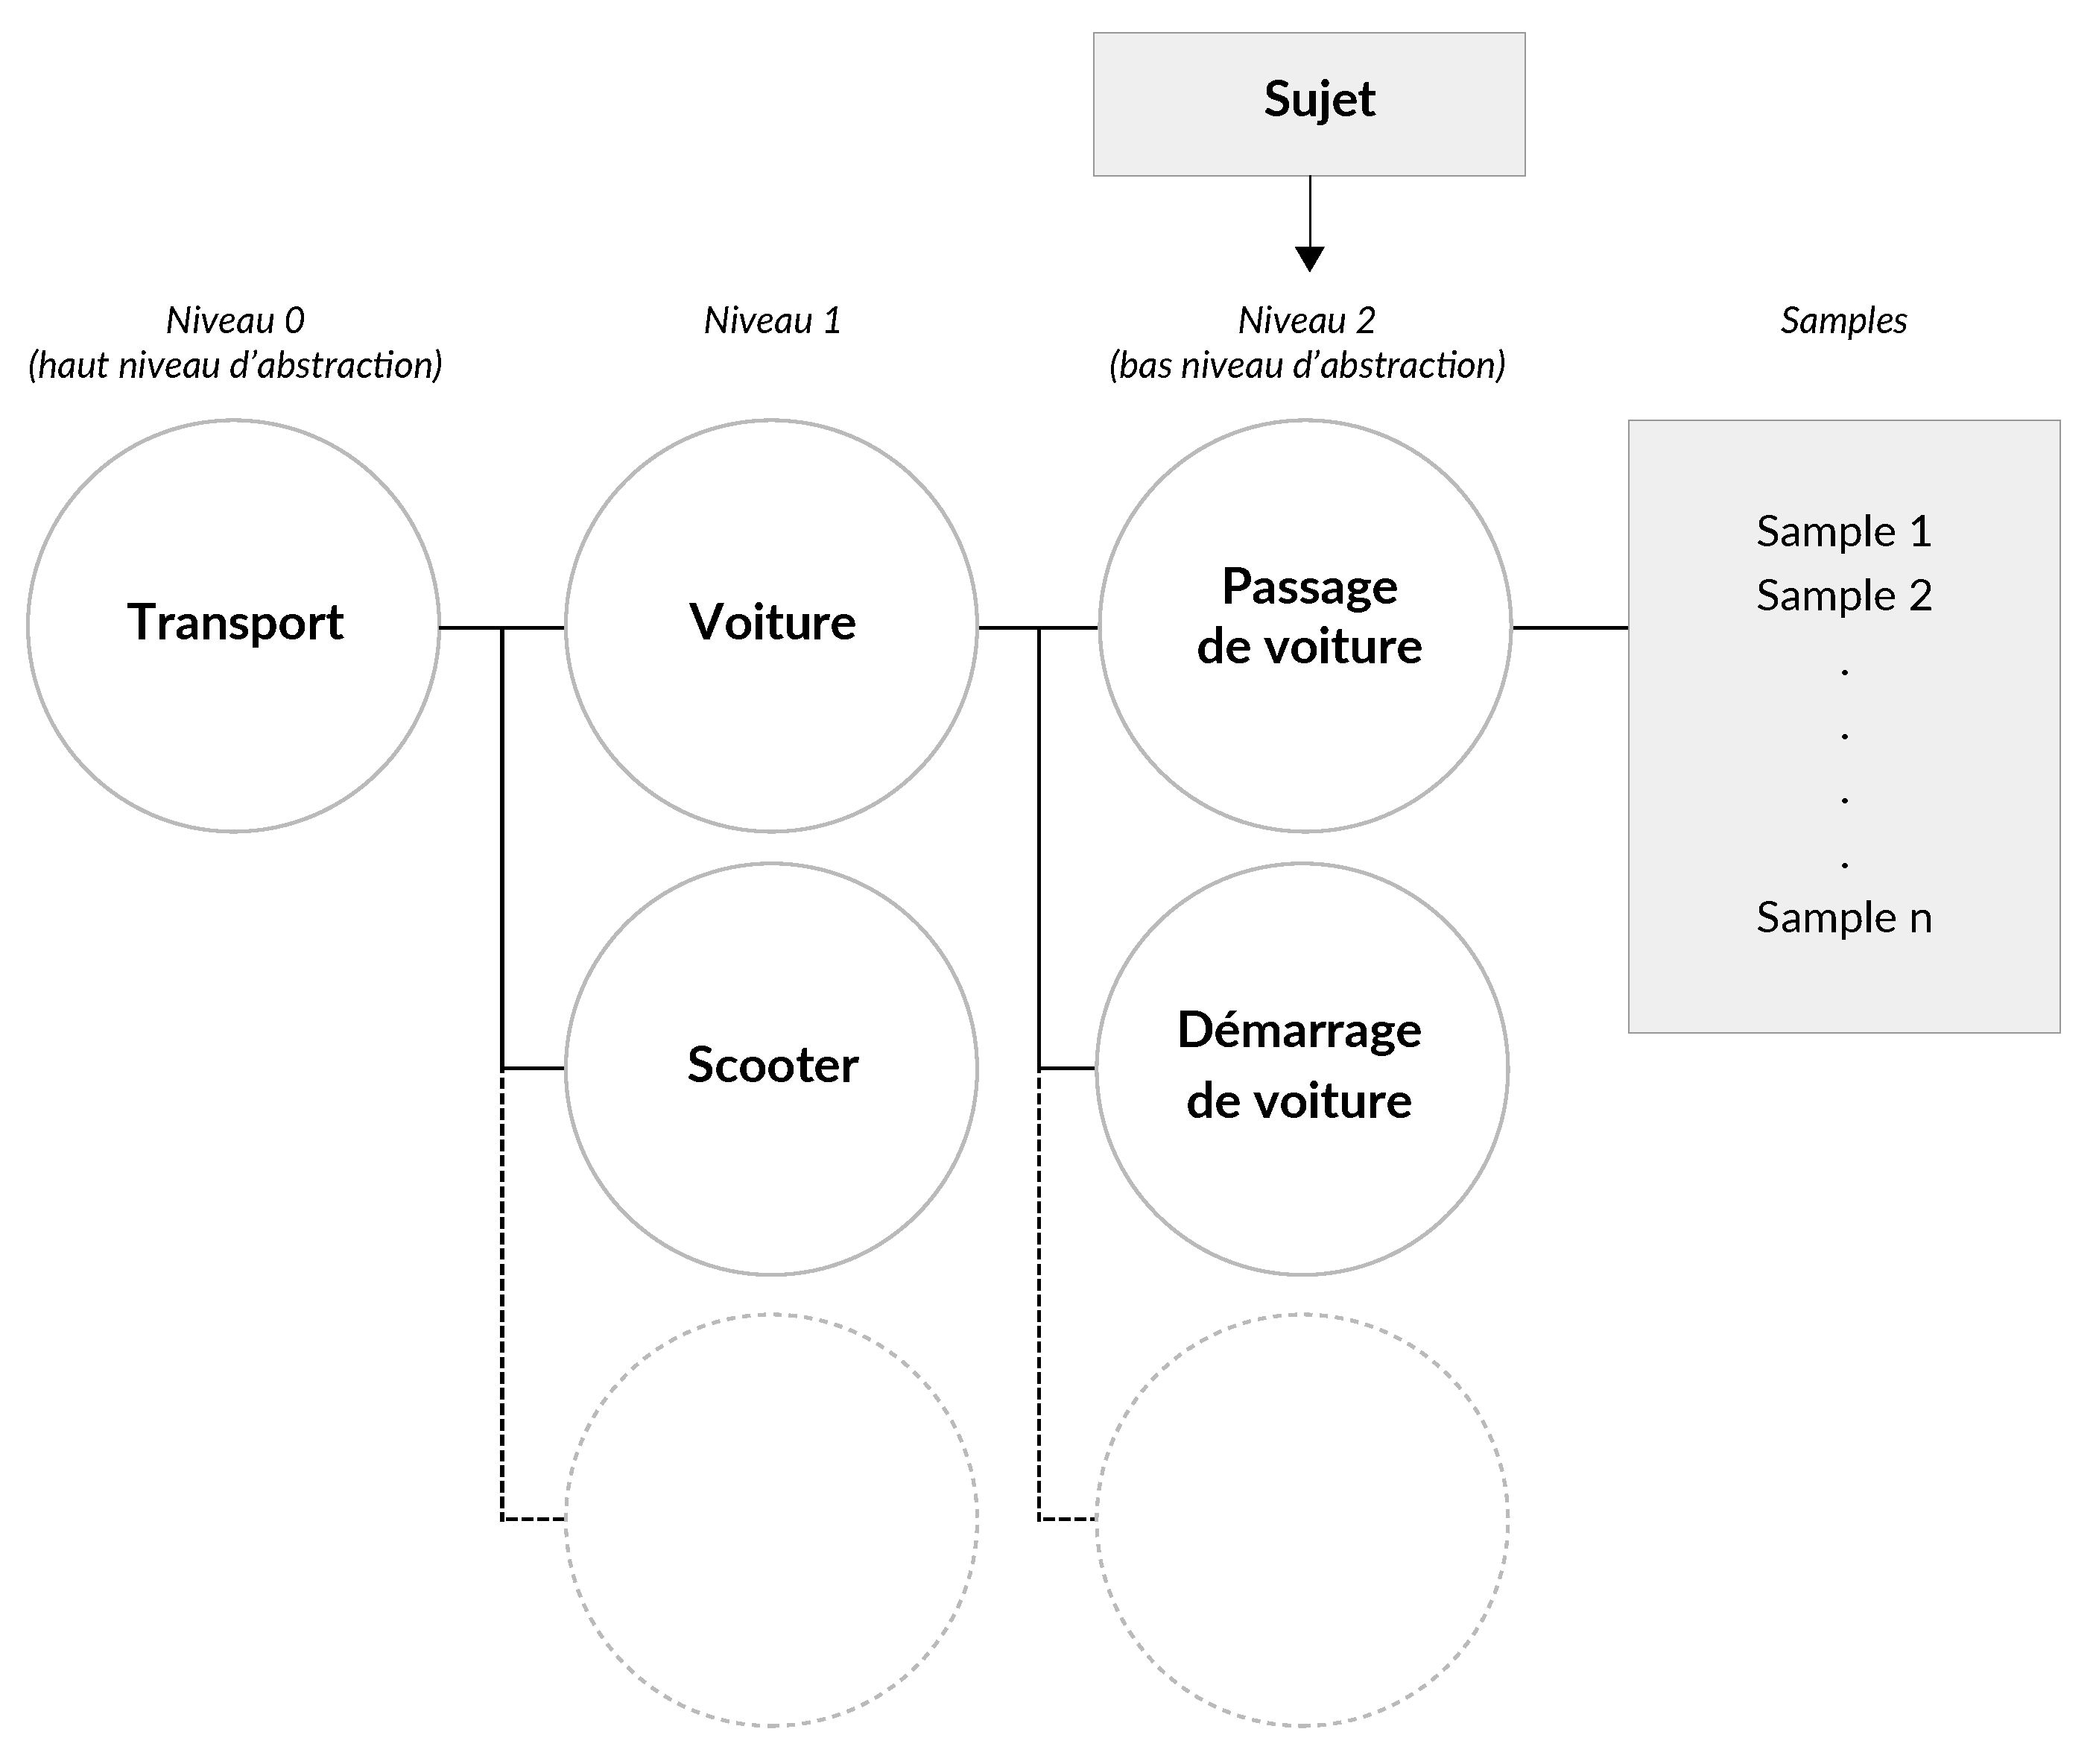
\includegraphics[width=.8\linewidth]{gfx/3.pdf}
       \caption{Hierarchical organisation of the isolated sounds used in the simulation.\gl{TODO : translate and remove subject box}}\label{fig:orgDb}
\end{figure}

%Nous nommons sample, un enregistrement d'un son isolé, événement ou texture. Chaque classe est alors comprise comme une collection de samples jugés perceptivement équivalents.

We term "sample", a recording of an isolated sound, be it an event or a texture. Each sound class is implemented as a collection of samples perceived equivalently.

%Les classes de sons sont organisées suivant une structure hiérarchique (\cf~Figure~\ref{fig:orgDb}). Cette structure hiérarchique est largement inspirée de l'axe vertical de l'organisation catégorielle proposée par E. Rosch \cite{rosch1978cognition}, qui dresse une taxonomie des classes ou catégories \ie~plus le niveau d'abstraction de la classe est faible, plus la description de la classe est précise, et plus les sources sonores incluses dans cette classe sont semblables. Si le niveau d'abstraction d'une classe est tel que cette dernière possède des sous-classes, alors sa collection de samples est la somme des collections respectives de chacune des sous-classes.

The sound classes are organized hierarchically (\cf~Figure~\ref{fig:orgDb}) according to a structure that is close to the one of the vertical axis of the categorical organization proposed by E. Rosch \cite{rosch1978cognition}. The lower the level of abstraction, the more precise the description of the class and the more perceptually similar the sound sources. For classes with high level of abstraction that have sub classes, their collection of samples is the union of the collections of the sub classes.

%Nous établissons deux taxonomies, une pour les événements, une autre pour les textures (\cf~Annexe~\ref{app:taxonomie}). Pour les événements, nous considérons quatre niveaux d'abstraction allant des classes les plus générales (niveau d'abstraction 0), aux classes les plus spécifiques (niveau d'abstraction 3). Pour les textures, nous ne considérons que trois niveaux d'abstraction. Notons que la taxonomie des événements est proche de celle de \cite{Salamon14}, introduite postérieurement à notre étude.

Accounting for the perceptual matters detailed previously, two taxonomies are built, one for event sounds and one for texture sounds. Four levels of abstraction are considered from the more generic one (level 0), to the more specific classes (level 2), leading to a taxonomy close to the one used in \cite{Salamon14}. Only three levels of abstraction are considered for the texture sounds.

\subsubsection*{Sound samples collection}

%Sur la base des taxonomies précédemment établies, 483 sons isolés ont été collectés, dont 381 événements, et 102 textures. Parmi ces samples, 332 ont été enregistrés, et 151 proviennent de différentes banques de sons (\emph{SoundIdeas}\footnote{\emph{SoundIdeas}: \url{www.sound-ideas.com}} et \emph{Universal SoundBank}\footnote{\emph{Universal SoundBank}: \url{www.universal-soundbank.com}}).

483 isolated sounds are collected and organized with the two typologies discussed above, 381 events and 102 textures. Among those samples, 332 have been recorded and 151 have been taken from two sound libraries: \emph{SoundIdeas}\footnote{\emph{SoundIdeas}: \url{www.sound-ideas.com}} and \emph{Universal SoundBank}\footnote{\emph{Universal SoundBank}: \url{www.universal-soundbank.com}}.

%Tous les enregistrements ont été effectués à l’aide d'un micro canon \emph{AT8035}\footnote{\emph{Micro canon AT8035}: \url{eu.audio-technica.com}} relié à un enregistreur \emph{ZOOM H4n}\footnote{\emph{ZOOM H4n} : \url{www.zoom.co.jp/english/products/h4n}}. L’utilisation du micro canon nous permet d’isoler les événements sonores du bruit de fond urbain. Pour les textures, il nous permet d’éviter les événements sonores proches du preneur de son. Nous pouvons ainsi pointer des "zones sonores", en nous tenant à une certaine distance de ces dernières, afin de capter uniquement le bruit de fond émanant de la zone ciblée.

Original sounds have been recorded using a shotgun microphone \emph{AT8035}\footnote{\emph{Micro canon AT8035}: \url{eu.audio-technica.com}} plugged to a \emph{ZOOM H4n}\footnote{\emph{ZOOM H4n} : \url{www.zoom.co.jp/english/products/h4n}} recorder. The use of such a microphone allowed us to isolate as much as possible sound events of interest from the urban background. It also allowed us to avoid dominant sound sources while recording texture sounds by targeting distant areas with no dominant sound sources.

%Tous les sons ont été normalisés au même niveau $RMS$ de $-12$ $dB$ (FS), \ie. relativement à un niveau pleine échelle (\emph{relative to Full Scale}). Dans notre cas, ce niveau pleine échelle est de 1 Volt.

All samples are normalized to the same $RMS$ level of $-12$ $dB$ FS, \ie relative to Full Scale. In our case, the full scale level is set arbitrarily to 1 Volt.

\subsection{Parameters}
\label{sec:simscene_parametre}

%Par choix de conception, l'outil de simulation ne permet pas d’interagir avec un sample en particulier, mais toujours avec une piste, \ie~une séquence de samples. Plusieurs paramètres permettent au sujet de contrôler la structure de chaque piste.

By a voluntary design choice, the simulation tool does not allow the user to interact and control directly a specific sample. Interaction is done at the track level, a track being a sequence of samples. Several parameters are available to the subject to control the track:

% \begin{itemize}
% \item \emph{niveau sonore} ($dB$): pour chaque sample, les niveaux sont tirés aléatoirement à partir d'une distribution normale, paramétrée par le sujet en termes de moyenne et de variance;
% \item \emph{espacement inter-onset} (seconde): (piste d'événements seulement) comme pour les niveaux, les espacements sont tirés aléatoirement à partir d'une distribution normale, paramétrée par le sujet en terme de moyenne et de variance;
% \item \emph{début et fin} (seconde): le sujet fixe le début et la fin de chaque piste.
% \end{itemize}

\begin{itemize}
\item \emph{sound level} ($dB$): for each sample, the sound levels are randomly sampled according to a normal distribution parametrized by the subject in terms of mean value and variance;
\item \emph{inter-onset spacing} (second): for the event's track only, and for each sound event sample, the inter-onset spacings are randomly sampled according to a normal distribution parametrized by the subject in terms of mean value and variance;
\item \emph{start and end time} (second): the subject set the first and last occurrence of a sample of the selected class.
\end{itemize}

%Afin de faciliter la simulation, deux paramètres supplémentaires sont proposés:

To improve simulation quality, two parameters are also proposed:

% \begin{itemize}
% \item \emph{fondu par événement} (seconde): (piste d'événements seulement) le sujet fixe une durée de fondu (entrée et sortie) appliquée à chaque sample;
% \item \emph{fondu global} (seconde): le sujet fixe les durées de fondus pour l'entrée et la sortie de la piste. Ces fondus s'appliquent ainsi à l'ensemble des samples de la piste.
% \end{itemize}

\begin{itemize}
\item \emph{event's fades} (seconds): for the event's track only, the subject can set a fade in / fade out duration applied to each sample;
\item \emph{global fades} (seconds): the subject can set global fade in / fade out duration applied to the entire track.
\end{itemize}

%Deux de ces paramètres ne s’appliquent que pour les pistes d'événements (\emph{fondu par événement}  et \emph{espacement inter-onset}), les samples des textures étant séquencés sans espacement.

The samples of texture are sequenced without time spacing, therefore the parameters \emph{event's fade} and \emph{inter-onset spacing} are not available for this kind of track.

\subsection{Selection interface}
\label{sec:simscene_ssf}

\begin{figure}[!tp]
		\myfloatalign
        \subfloat[]
        {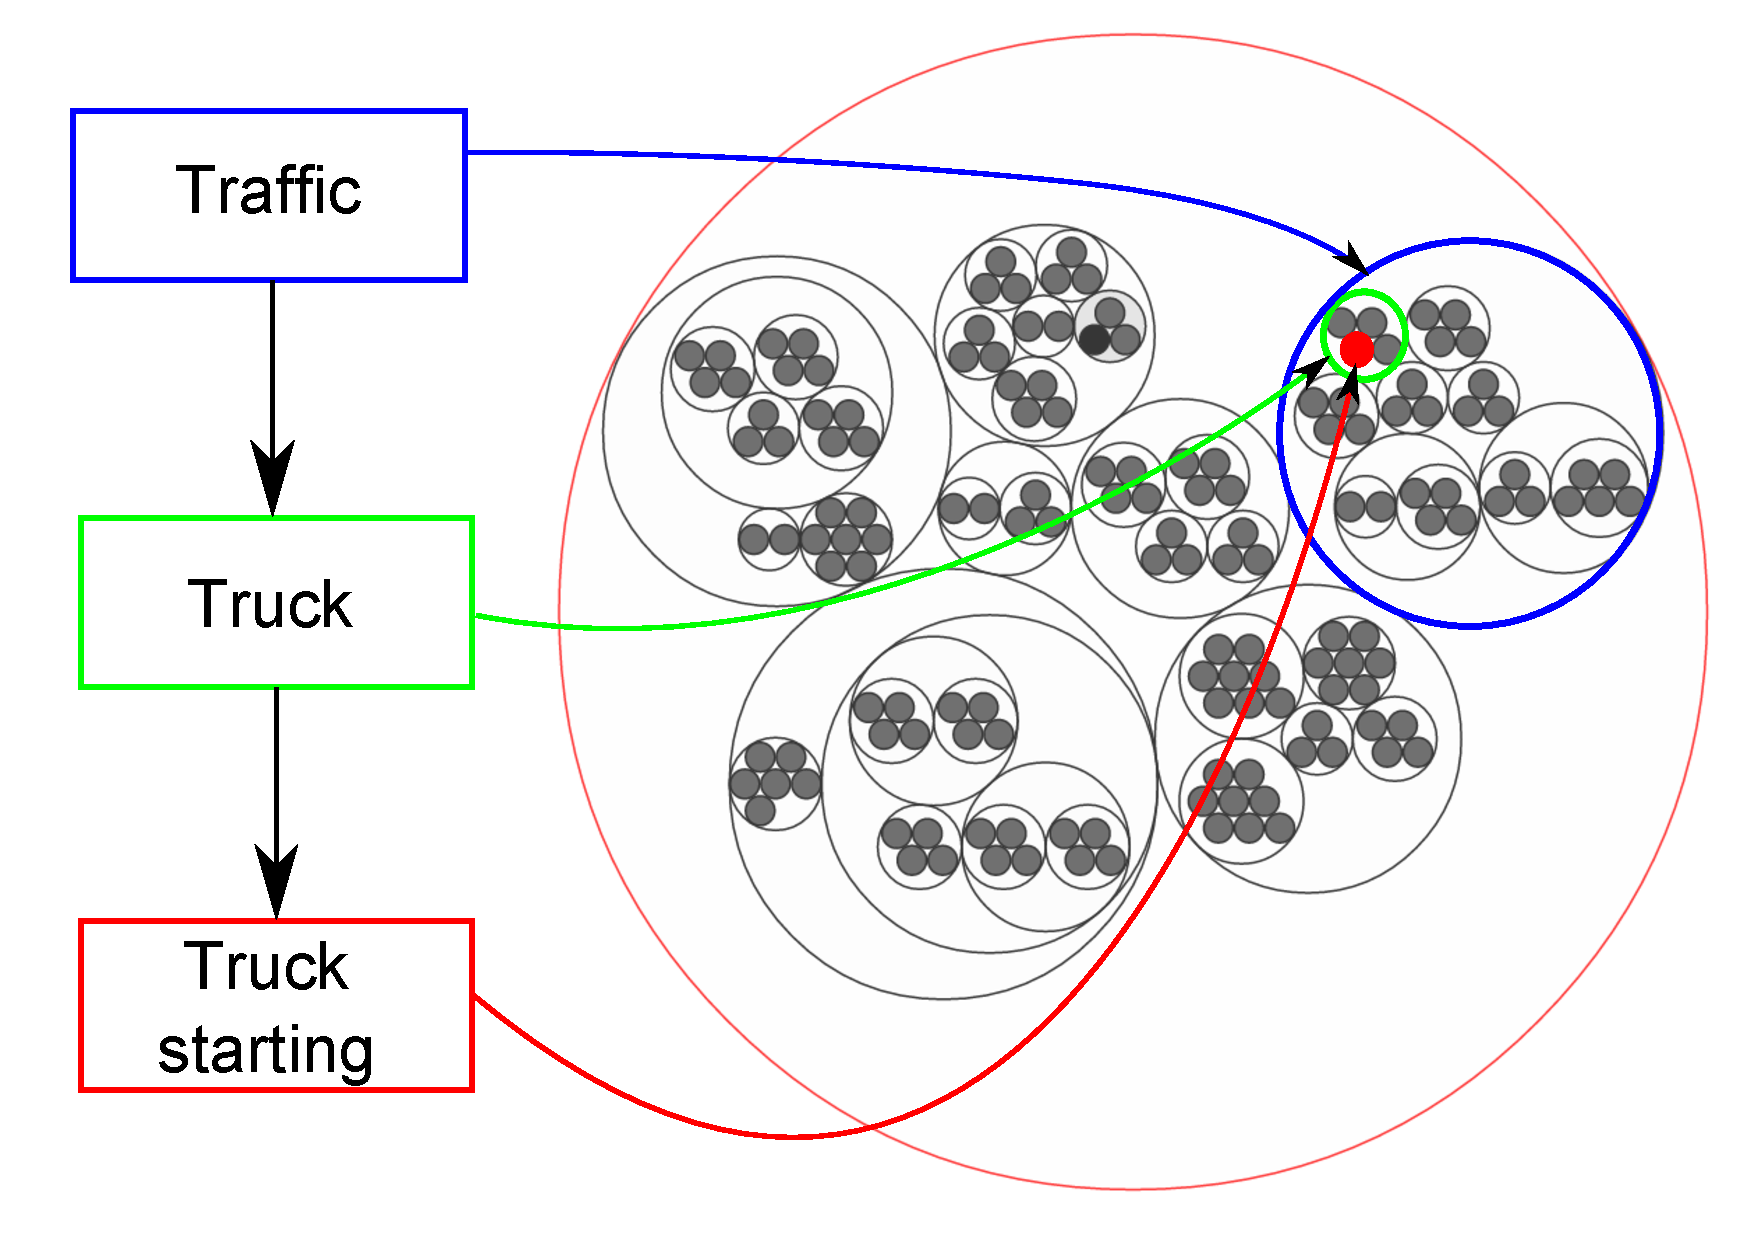
\includegraphics[width=.8\linewidth]{gfx/SSF}\label{fig:ssf}} \par
        \subfloat[]
        {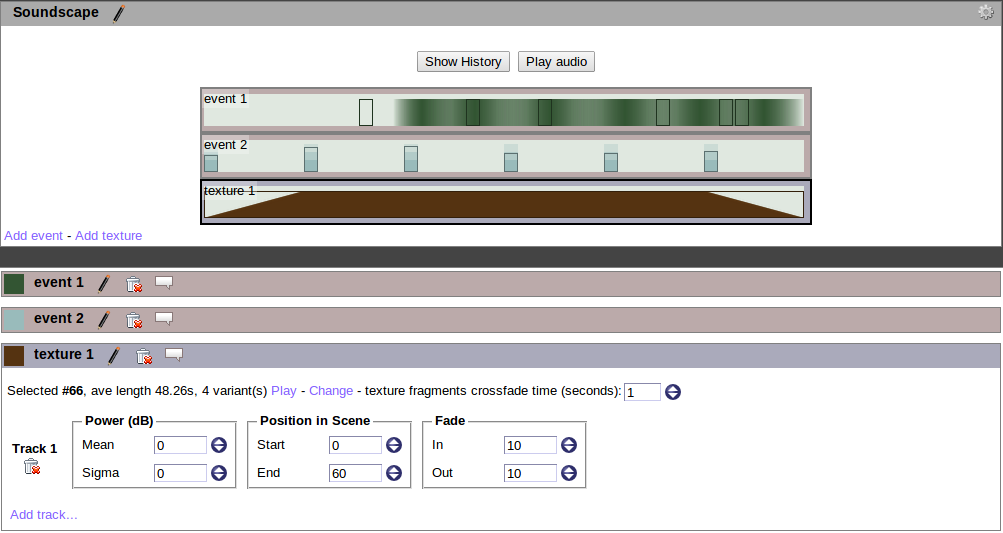
\includegraphics[width=\linewidth]{gfx/simscene}\label{fig:simscene}}
       \caption{Graphical interfaces for the selection of sound classes (a) and their sequencing (b) of the \emph{simScene} tool.}
\end{figure}

%La grande majorité des outils permettant de parcourir une banque de données propose une recherche textuelle sur la base de mots-clé. Dans le cadre d'une expérience sensorielle visant à objectiver la représentation interne du sujet, cette approche est problématique.

%En effet la description verbale du son, si elle est accessible au sujet, peut potentiellement influencer sa sélection. Dans les faits, pour construire une scène environnementale «~calme~», le sujet sélectionne a priori les sons référencés sous le vocable \emph{parc}.

Once the typology and the set of sounds are available, an important design issue is the need of a suitable way to display the sound dataset to the user. Most browsing tools are based on keyword indexing. However, for sensory experiment that study the objectivation of the mental representation of the subject, this mean is problematic as the availability of a verbal description of the sound can influence the choice of the subject and potentially induce biases in the analysis conclusions. Indeed, the subject may select \textit{a priori} sounds referenced as belonging to \emph{park} to build a \emph{calm} soundscape.

%Pour limiter l’influence de l’interface sur le sujet, il nous paraît nécessaire de libérer sa recherche de toute information textuelle. Nous proposons à l'utilisateur une interface graphique lui permettant d’explorer la banque de sons exclusivement à partir de l’écoute.

Therefore, the selection interface considered in this study is text free and composed of spatially organized circles on a plane, each representing one leaf class.

%La figure~\ref{fig:ssf} présente l'interface pour la banque de données d'événements sonores. Visuellement, les classes du dernier palier (niveaux d'abstraction 3 pour les événements, 2 pour les textures) sont représentées par des cercles, et positionnées sur un plan. La disposition des cercles dans l'espace dépend de l’organisation hiérarchique de la base de données: les sous-classes appartenant à une même classe sont proches les unes des autres, et ainsi de suite jusqu'à atteindre les classes du dernier palier, les seules auxquelles le sujet peut accéder, des classes qui ne possèdent pas de sous-classes, et sont directement liées à une collection de samples.

The Figure~\ref{fig:ssf} shows the interface used for the selection of events. The classes of the higher level of abstraction are plotted with circles. The spatial location of the circles is chosen according to the hierarchical organization of the sound database: sub-classes belonging to the same class are close to each others, and so on until the user reaches the lower level classes displayed in grey which are directly linked to a collection of samples.

%Chaque classe du dernier palier possède un son prototype. Ces sons ont été choisis par les expérimentateurs. Lorsqu’on clique sur un cercle, le prototype associé à la classe est joué. Le sujet parcourt la banque de sons en cliquant sur les cercles. Cette interface a fait l'objet d'une étude approfondie dont les résultats sont publiés dans \cite{lafay2016JAES}.

Each of those classes have a representative sound chosen arbitrarily by the authors in order to provide the same sound each time the user clicks on the circle. The subject can browse the database by listening to those prototype sounds. The efficiency of this interface compared to several others designs have been evaluated and the outcomes are discussed in \cite{lafay2016JAES}.

\subsection{Simulation interface}

%L'interface de simulation propose un rendu graphique schématisé de la scène en cours de création (\cf~Figure~\ref{fig:simscene}). La piste est représentée par une bande possédant un axe temporel. Sur cette bande, chaque sample est représenté par un rectangle. L'espacement entre les rectangles est fonction de l'espacement entre les samples. De même, la hauteur des rectangles est proportionnelle au niveau sonore des samples. Dans le cas d'une piste de texture, un unique rectangle apparaît sur toute la longueur de la piste, un son de texture ne pouvant être entrecoupé de silences. Les caractéristiques des rectangles évoluent en fonction des changements de paramètres de la piste. L'utilisateur a la possibilité, à tout moment, d'écouter la scène simulée.

As shown on Figure~\ref{fig:simscene}, the simulation interface displays a schematic of the scene under creation. Each track is represented as an horizontal band with a temporal axis. Each sample of this track is displayed by a rectangle whose height is proportional to the amplitude of the sample. For event's tracks, the horizontal spacing between those rectangles is a function of the time delay between their onsets. For tracks of texture, a unique rectangle is displayed as this kind of sounds does not allow spacing with silence. As actual amplitude and spacing values are drawn from random variables, each time the subject changes the value of a parameter, the location and height of the rectangles are updated to reflect the changes in the sequencing of the samples. The subject can listen to the resulting sound scene at any time.

%La scène sonore est ainsi vue comme une somme de sources sonores, ou, si l'on admet la distinction opérée entre événements et textures sonores, «~un squelette d'événements sur un lit de textures~» \cite{nelken2013ear}. Cet outil de simulation est présenté en détail dans \cite{rossignol2015simscene}.

As such, the underlying model of the scene is a sum of sound sources. Further details about the simulation interface can be found in \cite{rossignol2015simscene}.


%%%%%%%%%%%%%%%%%%%%%%%%%%%%%%%%%%%%%%%%%%%%%%%%%%%%%%%%%%%%
%%%%%%%%%%%%%%%%%%%  Experience 1     %%%%%%%%%%%%%%%%%%%%%%
%%%%%%%%%%%%%%%%%%%%%%%%%%%%%%%%%%%%%%%%%%%%%%%%%%%%%%%%%%%%


\section{Experiment 1}
\label{sec:simulation}

\subsection{Objective}

\begin{figure}[t]
        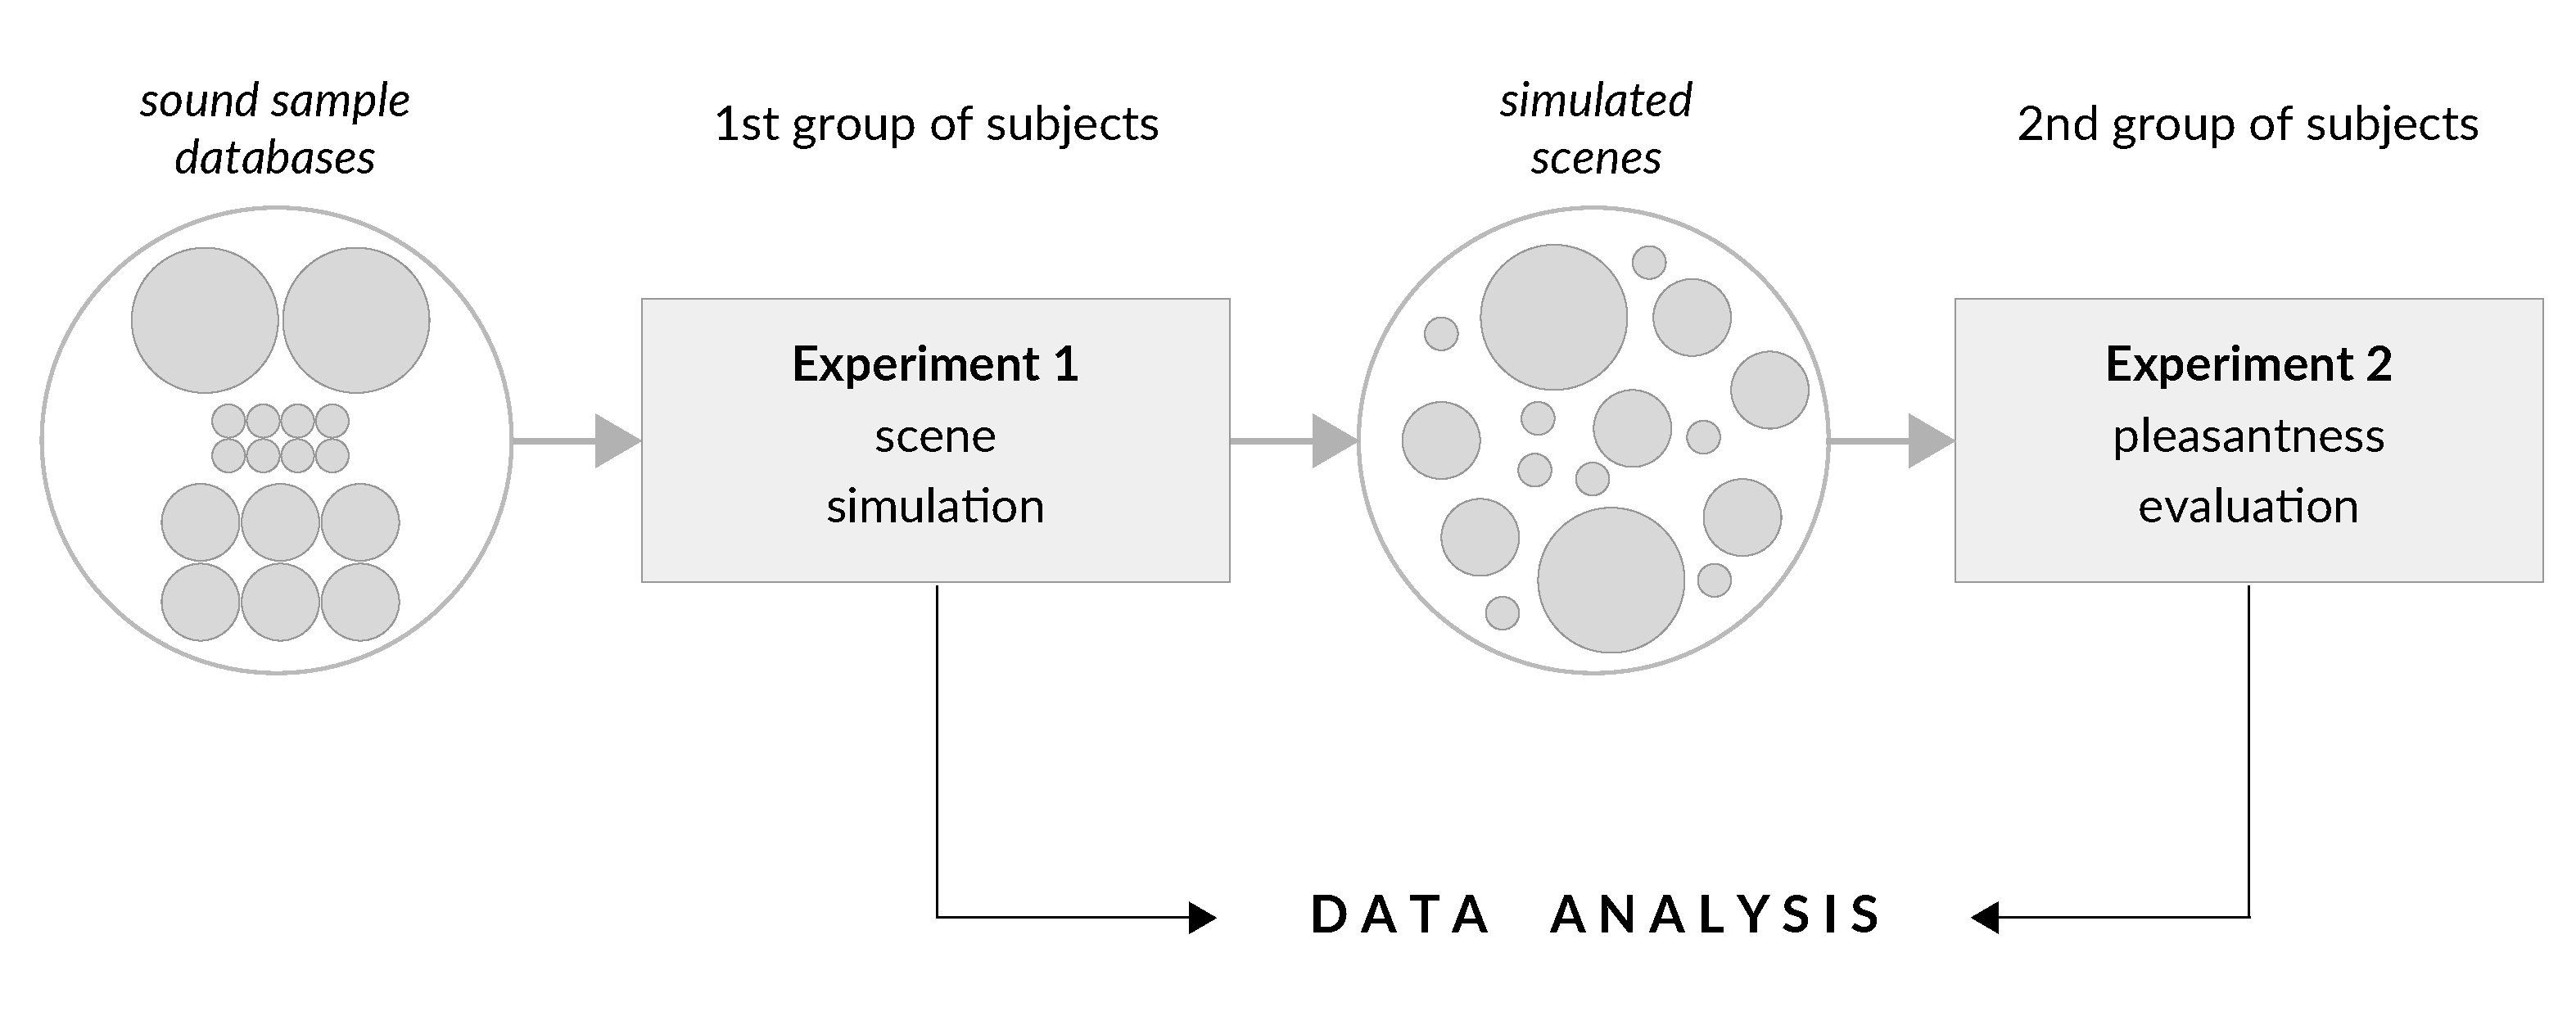
\includegraphics[width=\linewidth]{gfx/5.pdf}
        \caption{Experimental protocol of the simulation experiment (1.a) and the pleasantness evaluation experiment (1.b).\gl{TODO : translate}}\label{fig:xp1_2}
\end{figure}

% L'objectif est d'étudier les influences spécifiques des différentes sources sonores qui composent les environnements urbains sur la perception de l'agrément, en utilisant la simulation. Pour ce faire, nous planifions nos deux premières expériences (\cf~Figure~\ref{fig:xp1_2}):

Experiment 1 aims at using a simulation paradigm to investigate the specific influences of the various sound sources constituting urban soundscapes on the perceived pleasantness. For that, the two first experiments are planned as follows (\cf~Figure~\ref{fig:xp1_2}):

% \begin{itemize}
% \item \emph{expérience 1.a de simulation}: au cours de cette expérience, les sujets doivent simuler des environnements sonores urbains, en utilisant l'outil de simulation \emph{Simscene} (\cf~Section~\ref{sec:simscene}). Chacun compose deux environnements sonores, le premier idéal/agréable et le deuxième non-idéal/désagréable.
% \item \emph{expérience 1.b d'évaluation}: à l'issue de la simulation, nous n'avons, de fait, qu'une connaissance binaire des propriétés affectives des scènes simulées: idéale (i) et non-idéale (ni). Cette seconde étape a pour but d'affiner notre connaissance sur l'agrément. Pour ce faire, nous demandons à un deuxième groupe de sujets d'évaluer, à partir d'une échelle sémantique, l'agrément de chacune des scènes simulées. L'expérience d'évaluation sert deux buts:
% \begin{enumerate}
% \item évaluer l'influence respective des différentes sources sur l'agrément, pour chaque type d'environnement (i ou ni);
% \item détecter la présence de cas extrêmes ou ambigus (\emph{outlier}) dans les scènes simulées. Pour le reste de notre étude, les qualités hédoniques imposées (i et ni) servent de référence, de vérité terrain. Il nous faut donc garantir qu'il n'y ait pas d’ambiguïté entre les cas extrêmes des i- et ni-scènes, \ie~que la note d'agrément la plus basse des i-scènes reste supérieure à la note la plus haute des ni-scènes.
% \end{enumerate}
% \end{itemize}

\begin{itemize}
\item \emph{experiment 1.a (simulation)}: during this experiment, subjects are asked to simulate urban sound environments, using the simulation tool \emph{Simscene}, see Section~\ref{sec:simulator}. Each of them has to create two sound environments: one ideal / pleasant and the other one, non ideal / unpleasant.
\item \emph{experiment 2.a (evaluation)}: after the simulation phase, only a binary information on the pleasantness property of the respective scenes is available: respectively ideal (i) or non ideal (ni). Furthermore, this information is given by the creator of the scene. The second experimental step aims at investigating more deeply and more broadly our knowledge on the pleasantness of the simulated scenes. For that, a second group of subjects is asked to evaluate the pleasantness of each scene, on a semantic scale. This experiment has two goals:
\begin{enumerate}
\item to evaluate more precisely the respective influence of the various sources composing the scenes on the pleasantness  (i or ni) thanks to a finer quantification of the pleasantness of the scene.
\item to detect the presence of \emph{outliers} or ambiguous scenes. Indeed, throughout our analyses, the predefined hedonic properties of the scenes (i and ni) are used as reference. We thus need to ensure beforehand that no ambiguity exists between extreme cases of i and ni scenes, \ie~that the less pleasant i-scene remains above the more pleasant ni-scene.
\end{enumerate}
\end{itemize}

% Notre analyse s'appuie sur les données produites par les deux expériences.

The data collected by these two experiments (1.a and 1.b) are analyzed conjointly.

\subsection{Planning of Experiment 1.a}
\label{sec:xp1a_plan}

The design of this experiment has been validated with a pilot study described in \cite{lafay2014new}.

\subsubsection*{Procedure}

% Les sujets doivent simuler deux environnements sonores urbains, chacune des scènes devant durer 1 minute. Ils doivent se conformer aux consignes suivantes:

The subjects have to simulate two urban sound environments of one minute each. They follow the instructions below:

% \begin{itemize}
% \item première simulation: simuler un paysage sonore \textbf{urbain plausible} qui, selon vous, est idéal (où vous aimeriez vivre);
% \item deuxième simulation: simuler un paysage sonore \textbf{urbain plausible} qui, selon vous, est non-idéal (où vous n'aimeriez pas vivre).
% \end{itemize}

\begin{itemize}
\item  first simulation: create a \textbf{plausible urban soundscape} which is ideal, according to you (where you would like to live);
\item second simulation: create a \textbf{plausible urban soundscape} which is non ideal, according to you (where you would not like to live);
\end{itemize}

% Tous commencent par simuler l'environnement idéal. Ils ne prennent connaissance de la deuxième consigne qu'à la fin de la première simulation.

% Les sujets sont totalement libres dans le choix des sons, et des paramètres. Ils doivent cependant se soumettre à deux contraintes:

All the subjects start by designing the ideal environment; they read the second set of instructions at the end of the first experiment. subjects are completely free of their choices concerning sounds and synthesis parameters. The created sound environments must nevertheless fulfill the two following constraints :

% \begin{itemize}
% \item le sujet doit prendre le point de vue d’un auditeur fixe;
% \item le paysage sonore doit être réaliste, au sens de physiquement plausible. Le sujet peut très bien réunir 10 chiens dans un paysage sonore. Il ne peut en introduire 1 qui aboierait toutes les 10 millisecondes.
% \end{itemize}

\begin{itemize}
\item the listening point of view is the one of a fixed listener;
\item the soundscape must be realistic, \ie~physically plausible. For instance, subjects are free to insert ten dogs in the soundscape but they cannot insert one dog barking every 10 milliseconds.
\end{itemize}

% Ces contraintes font partie de la consigne. Aucun contrôle n'est fait \emph{a priori} dans l'interface de simulation.

These constraints are notified in the instructions; no control is done \emph{a priori} in the simulation interface.

% Chaque processus de simulation comprend deux parties :
%
% \begin{enumerate}
% \item la réalisation de la simulation: cette étape se décompose en trois temps:
% \begin{itemize}
% \item sélectionner les classes de sons
% \item nommer les classes de sons sélectionnées
% \item paramétrer les pistes (\cf~Section~\ref{sec:simscene_parametre}) relatives aux classes de sons sélectionnées
% \end{itemize}
% \item la production d'un commentaire libre du paysage sonore simulé
% \end{enumerate}

Each simulation process is decomposed in several steps:

\begin{enumerate}
\item the simulation: the user is asked to:
\begin{itemize}
  \item  select the class of sounds
	\item  give a name to the selected class of sounds
	\item  set the parameters of the tracks related to the selected class of sounds, see Section~\ref{sec:simscene_parametre}.
\end{itemize}
\item the feedback : writing of a free form comment about the composed soundscape
\end{enumerate}

% En complément, et une fois les deux scènes sonores réalisées, les sujets sont invités à:
%
% \begin{itemize}
% \item indiquer les sources sonores qu'ils voulaient mettre, mais qu'ils n'ont pas trouvées;
% \item commenter l’ergonomie du logiciel de simulation;
% \item commenter l’ergonomie de l'interface de sélection.
% \end{itemize}

In addition, once the two sound scenes are completed, subjects are invited to:

\begin{itemize}
\item  point out the sound sources that were missing for the composition
\item  give a comment about the ergonomics of the simulation environment
\item   give a comment about the ergonomics of the selection tool
\end{itemize}

% Avant de commencer la première simulation, un tutoriel de 20 minutes est proposé aux sujets, afin qu'ils se familiarisent avec le logiciel de simulation, et la banque de données. L'expérience est prévue pour durer 2h30.

Before starting the first simulation, a 20-minute tutorial is given to the subjects in order to familiarize them with the simulation interface and the sound database. The experiment is planned to last about two hours and a half, including breaks that the subjects are allowed to take.

\subsubsection*{Apparatus}

% Tous les sujets passent l'expérience sur des machines identiques. L'audio est diffusé en diotique, par le biais de casques audio. Pendant le tutoriel, les sujets doivent ajuster le niveau sonore à un volume confortable. Ils ne peuvent le modifier par la suite.

All the subjects perform the experiment on standard desktop computers with the same hardware and software configurations. The audio files are played in diotic conditions using headphones. During the tutorial, subjects are asked to adjust the sound volume to a comfortable level. Once set, they are not allowed to modify it during the remaining of the experiment.

% Tous les sujets réalisent l'expérience simultanément. Ils sont répartis de manière égale dans trois pièces identiques, toutes possédant un environnement calme. Ils n'ont pas le droit de s'adresser la parole pendant l'expérience.

All the subjects performed the experiment at the same time. They are equally distributed in three identical quiet rooms. They are not allowed to talk to each other during the experiment.

% Trois expérimentateurs, un dans chaque pièce, sont présents durant la totalité de l'expérience, afin de contrôler le bon déroulement de cette dernière, et de répondre aux éventuelles questions des sujets.

Three experimenters (one in each room) are available during the whole duration of the experiment in order to assist subjects with potential hardware and software issues and to answer questions.

\subsubsection*{subjects}

% 44 étudiants (14 femmes) de L’École Centrale de Nantes ont participé à l'expérience. Ils ont tous sensiblement le même âge (moyenne: 21.6, écart-type: 2). Tous les sujets sont Nantais, et vivent dans cette ville depuis deux ans ou plus.

44 students (14 females; averaging $21.6$ years of age, s.d. of $2.0$ years) from \emph{Ecole Centrale de Nantes} (a french engineering school) took part to the experiment. All the subjects live in Nantes, France, for at least two years.

% Sur les 44 sujets, 40 réalisent l'expérience avec succès, produisant au final 80 scènes sonores simulées, dont 40 scènes idéales, et 40 scènes non idéales. 4 sont éliminés pour non respect ou incompréhension des consignes, d'une part, et dépassement du temps, d'autre part.

Among the 44 subjects, 40 succeeded, producing at the end 80 simulated sound scenes (40 ideal scenes, 40 non ideal scenes). the 4 other subjects were excluded from the process due to a lack of understanding of the instructions or failure to respect them, or for exceeding the maximum duration allowed to perform the experiment.

\subsection{Planning of experiment 1.b}
\label{sec:xp1b_plan}

\subsubsection*{Procedure}

% En raison de contraintes temporelles, les sujets n'évaluent que des séquences de 30 secondes des scènes simulées, chacune de ces séquences commençant à la seconde 15, et finissant à le seconde 45 de la scène d'une durée initiale de 1 minute.

Due to temporal constraints, subjects only assess 30 seconds of the initial 1-minute simulated scenes generated in experiment 1.a (from sec. 15 to sec. 45).

% L'évaluation s'effectue sur une échelle sémantique bipolaire de 7 points, allant de -3 (non-idéale/très désagréable) à +3 (idéale/très agréable). Avant de noter une scène, les sujets doivent obligatoirement écouter les 20 premières secondes de cette dernière. Après la notation, ils sont libres de passer à la scène suivante.

The assessment is done with a 7-point bipolar semantic scale going from -3 (non ideal / unpleasant) to +3 (ideal / pleasant). Before evaluating a scene, subjects must listen to the first 20 seconds of the stimuli. After the evaluation, they are free to continue to the next scene.

% Pour chaque sujet, les scènes sont présentées dans un ordre aléatoire. Les 10 premières scènes permettent au sujet de calibrer ses notes. Elles sont obligatoirement composées de 5 scènes idéales, et de 5 scènes non-idéales. Ces 10 premières scènes sont rejouées à la fin de l'expérience, et seules les notes données à la deuxième occurrence sont prises en compte.

For each participant, sound scenes are played in a quasi random order. 5 ideal scenes and 5 non ideal scenes are first sequenced to allow the subjects to calibrate their scores. These first 10 scenes are played back again at the end of the experiment. Only the last evaluations are taken into account.

% L'expérience est prévue pour durer 30 minutes. Les sujets ne connaissent pas la nature des scènes.

The experiment is planned to last 30 minutes. The subjects do not know anything beforehand about the nature of the sound scenes.

\subsubsection*{Apparatus}

% Tous les sujets passent l'expérience sur des machines identiques. L'audio est diffusé en monophonie, par le biais de casques audio semi-ouverts \emph{Beyer-Dynamic DT 990 Pro}. Toutes les scènes sonores ont été re-simulées sur la base des partitions obtenues lors de l'expérience de simulation. Le niveau sonore de sortie est identique pour tous les sujets.

All the subjects perform the experiment on computers with equivalent hardware and software configurations. The audio files are played in diotic conditions by semi-open headphones \emph{Beyerdynamic DT 990 Pro}. The stimuli are the scenes obtained by the simulation experiment of experiment 1.a. The output sound level is the same for all the subjects.

% Tous les sujets réalisent l'expérience simultanément, dans un environnement calme. Ils n'ont pas le droit de s'adresser la parole pendant l'expérience.

All the subjects perform the experiment simultaneously. They are not allowed to talk to each other during the experiment.

% Un expérimentateur est présent durant la totalité de l'expérience, afin de contrôler le bon déroulement de celle-ci, et de répondre aux éventuelles questions des sujets.

An experimenter is available during the whole duration of the experiment in order to assist subjects and answer questions any questions the subjects may have.

\subsubsection*{subjects}

% 10 étudiants (2 femmes) de L’École Centrale de Nantes ont participé à l'expérience. Aucun d'entre eux n'a réalisé l'expérience de simulation. Tous les sujets ont sensiblement le même âge (moyenne: 23.1, écart-type: 1.8). Tous les sujets sont Nantais, et vivent dans cette ville depuis deux ans ou plus.

10 students (2 females; averaging $23.1$ years of age, s.d. of $1.8$ years) from \emph{Ecole Centrale de Nantes} (a french engineering school) took part to the experiment. All the subjects live in Nantes, France, for at least two years. None of them took part to the previous simulation experiment (experiment 1.a).

% Tous les sujets ont réalisé l'expérience avec succès.

All the subjects succeeded in doing the experiment.

\subsection{Data and statistical analysis}
\label{sec:xp1_dataAna}

\begin{table}[t]
\centering
\begin{tabular}{c c}
Terms                              & Acronyms                   \\
\hline
Sound level                        & $L$                        \\
Sound level (events)               & $L(E)$                     \\
Sound level (textures)             & $L(T)$                     \\
Average pleasantness (per scene)   & $\mathcal{A}_{scene}$      \\
Average pleasantness (per subject) & $\mathcal{A}_{subject}$      \\
                                   &                            \\
ideal/pleasant                     & i                          \\
non-ideal/unpleasant               & ni                         \\
scene ideal/pleasant               & i-scene                    \\
scene non-ideal/unpleasant         & ni-scene                   \\
\hline
\end{tabular}
\vspace{0.5mm}
\caption{Acronyms of features used in the analysis of the sensory experiments.}
\label{tab:acronyme}
\end{table}

% A chaque scène est associé un groupe de descripteurs. C'est sur ces descripteurs que nous pratiquons l'analyse. Un résumé de ces derniers, ainsi que des acronymes les désignant, est présenté dans le Tableau~\ref{tab:acronyme}. Afin de rester cohérent avec l’expérience 1.b d'évaluation, les descripteurs ne sont pas calculés sur la durée totale des scènes, mais sur la version réduite de 30 secondes (\cf~Section~\ref{sec:xp1b_plan}).

A set of features is attached to each sound scene. The analysis is done on the basis of these features. A summary of these features (and the corresponding acronyms) is presented in Table ~\ref{tab:acronyme}. In order to be consistent with the evaluation of experiment 1.b, features are not computed in the whole duration of the sequences but only on their 30-second reduced version used as stimuli for experiment 1.b, see Section~\ref{sec:xp1b_plan}.

% Pour chaque scène sonore, trois types de descripteurs sont considérés:

For each sound scene, three types of features are considered :

% \begin{itemize}
% \item \emph{perceptif}: il s'agit de l'agrément perçu de la scène simulée, évalué sur une échelle sémantique de 7 points. Nous notons $\mathcal{A}_{scene}$ l'agrément moyen d'une scène, obtenu en moyennant les notes de tous les sujets. De même, nous notons $\mathcal{A}_{sujet}$ l'agrément par sujet, en moyennant l'ensemble des notes de chacun. Compte tenu du faible nombre de sujets, nous faisons le choix, dans cette étude, de ne pas normaliser les notes d'agrément;
% \item \emph{sémantique}: il s'agit d'un vecteur booléen noté $S=(x_1,x_2,\ldots,x_n)$, indiquant les classes de sons présentes dans la scène. Chaque point $x$ de ce vecteur correspond à une classe de sons particulière: $x=1$ si la classe est présente dans la scène, et $x=0$ autrement. La dimension $n$ des vecteurs dépend du niveau d'abstraction considéré, \eg~pour le niveau d'abstraction 1, qui comprend $44$ classes de sons, cette dimension sera de $n=44$.
% \item \emph{structurel}: il s'agit du \emph{niveau Sonore}. Pour représenter le niveau sonore, nous nous inspirons de la mesure $L_{Aeq}$. Dans notre cas, il s'agit d'un scalaire calculé sur le signal en volts, et non en pression, et donné en décibels, en prenant un référentiel de 1 Volt. Le niveau est obtenu en calculant, toutes les secondes, la moyenne quadratique du signal, et en moyennant sur la durée de la scène. Un filtrage de type A est opéré avant le calcul des moyennes quadratiques. Nous notons $L$, $L(E)$ et $L(T)$ les niveaux calculés en tenant compte respectivement de l'ensemble des samples, des samples d'événements et de textures.
% \end{itemize}

\begin{itemize}
\item \emph{perceptual features}: the perceived pleasantness of the composed scene, assessed on a 7-point bipolar semantic scale. $\mathcal{A}_{scene}$ is the average pleasantness for one scene, as the average of the marks of all the subjects. $\mathcal{A}_{subject}$ is the average pleasantness for each participant, computed as the average of all the score given by each participant. Given the low number of subjects in experiment 1.b, we choose not to normalize the pleasantness scores.

\item \emph{semantic features}: we use a boolean vector $S = (x_1, x_2, \ldots, x_n)$ that indicates the class of sounds involved in the scene, \textit{i.e.} the sound classes that are present / absent from the scene. Each boolean $x$ of this vector corresponds to a specific class of sounds: $x = 1$ if the class is present in the scene, and $x = 0$ otherwise. The vector dimension ($n$) depends on the level of abstraction that is considered for the analysis. For instance, for the abstraction level 1 that includes 44 classes of sounds, $n = 44$.

\item \emph{sound levels}: to figure out the sound levels, we draw inspiration from the $L_{Aeq}$. In our case, it is a scalar computed from the  signal (in Volt and not in Pascal), and converted in decibels, with a reference of 1 Volt (full scale). The level is obtained by computing the quadratic mean of the signal every second and averaging the results over the total duration of the scene. An A-filtering module processes the data before the quadratic means are computed. We note $L$, $L(E)$ and $L(T)$ the computed levels by respectively considering the whole set of samples, only the set of event samples, and only the set of texture samples.
\end{itemize}

%Pour évaluer l'impact spécifique des différentes sources sonores sur l'agrément perçu, nous soumettons nos travaux aux 5 tests/études de significativité présentés ci-après:

In order to evaluate the specific impact of the various sound sources on the perceived pleasantness, we put the data to the five following significance tests:

\begin{itemize}

%\item \emph{vérification de l'agrément des scènes simulées}: afin de vérifier que la distinction affective imposée entre les i- et ni-scènes se retrouve au niveau de l'agrément perçu, nous observons s'il existe des différences entre les deux types de scènes au niveau de $\mathcal{A}_{scene}$ et $\mathcal{A}_{sujet}$. La significativité est évaluée par un test de Student à deux populations indépendantes pour $\mathcal{A}_{scene}$, et par un test de Student à deux populations appariées pour $\mathcal{A}_{sujet}$;

\item \emph{analysis of the perceived pleasantness}: the goal is to evaluate whether the perceived pleasantness is in accordance with the pleasantness label given by the creators of the  i- and ni-scenes during the experiment 1.a. To do so, we consider if there exist significant differences for the i- and ni-scenes of the average $\mathcal{A}_{scene}$ and the average $\mathcal{A}_{subject}$. The significance is evaluated by a two-sample Student test for $\mathcal{A}_{scene}$ and by a paired-sample Student test for $\mathcal{A}_{subject}$;

% GL comprends pas en francais

%\item \emph{analyse des descripteurs structurels}: afin d'évaluer si la distinction affective imposée entre les i- et ni-scènes impacte de manière significative la nature des scènes, \ie~s'il existe des différences significatives entre les descripteurs structurels, nous évaluons cette significativité à partir d'un test de Student à deux populations;

\item \emph{analysis of the sound levels}: the goal is to evaluate whether the sound levels differ between the i- and ni-scenes. The significance is measured with a two-sample Student test;

%\item \emph{étude de l'influence des descripteurs structurels sur l'agrément perçu}: afin d'évaluer l'impact potentiel des descripteurs structurels sur l'agrément perçu, nous étudions l'existence de corrélations linéaires entre ces descripteurs et $\mathcal{A}_{scene}$. Pour mesurer la corrélation, nous utilisons le coefficient de Pearson. Nous adoptons ici une méthodologie couramment utilisée dans l'approche dimensionnelle;

\item \emph{influence of the sound levels on the perceived pleasantness}: the goal is to evaluate if the sound levels impact the perceived pleasantness. To do so, we consider linear correlations between these features and $\mathcal{A}_{scene}$. The Pearson correlation coefficient is used for that purpose;

%\item \emph{analyse des descripteurs sémantiques}: afin d'apprécier si la distinction affective imposée a un impact sur la composition des scènes en terme de sources sonores, s'il est des classes de sons plus particulièrement utilisées pour simuler un type d'environnement (i ou ni), nous utilisons le V-test. Le test est effectué pour chaque niveau d'abstraction, et séparément, pour les classes d'événements et de textures. Pour chaque classe $j$ et chaque type d'environnement $k$ ($k=\lbrace i,ni\rbrace$), la valeur $V_{jk}$ du V-test se calcule comme suit:

%où $c$ est le nombre de classes utilisées, $c_k$ le nombre de classes utilisées pour un type d'environnement $k$, $c_j$ le nombre de classes $j$ utilisées, et $c_{jk}$ le nombre de classes $j$ utilisées pour un type d'environnement $k$. Le V-test teste l'hypothèse nulle que la proportion $\frac{c_{jk}}{c}$ ne diffère pas significativement de la proportion $\frac{c_{jk}}{c_k}$. Si pour un environnement $k$, et une classe $j$, l'hypothèse est rejetée, la classe $j$ est alors typique de l'environnement $k$. Les classes typiques sont nommées \textbf{marqueurs sonores};

\item \emph{analysis of the semantic features}: the goal is to evaluate if specific classes are more frequently used to simulate a given type of environment (i or ni). To do so, a V-test is considered \citep{rakotomalala2008tvpercent}. With $c$ being the total number of classes used for both types of environment, $c_k$ the number of classes used for a given type of scene $k$ ($k=\lbrace i,ni\rbrace$), $c_j$ the number of time a class $j$ has been used, and $c_{jk}$ the number of time a class $j$ has been used for a given type of scene $k$, the V-test evaluates the null hypothesis that the ratio $\frac{c_{jk}}{c}$ is not significantly different from the ratio $\frac{c_{jk}}{c_k}$. For each class $j$, and each environment type $k$, an approximation of the statistic value $V_{jk}$ is computed as follows:

\begin{equation}
V_{jk}=\dfrac{c_{jk}-c_k\frac{c_j}{c}}{\sqrt{c_k\frac{c-c_k}{c-1}\frac{c_j}{c}(1-\frac{c_j}{c})}}
\end{equation}

If the null hypothesis is rejected, the class $j$ is said to be typical with respect to the type of scene $k$. The typical classes are called \textbf{sound markers}. Testing is done for each class, at each level of abstraction, and separately for texture and event classes;

%\item \emph{étude des espaces de représentation induits par les descripteurs sémantiques}: afin d'étudier si une représentation basée uniquement sur la présence ou l'absence de classes de sons permet de séparer les deux types d'environnement, nous considérons l'espace induit par les descripteurs sémantiques $S$. $S$ étant un vecteur booléen, nous calculons les distances entre les scènes à partir de la distance de Hamming. Considérant les deux vecteurs $S_1=(x_{1,1},x_{1,2},\ldots,x_{1,n})$, et $S_2=(x_{2,1},x_{2,2},\ldots,x_{2,n})$ de dimension $n$, avec $x=\lbrace 0,1\rbrace$, la distance de Hamming $d_{ham}$ mesure le pourcentage de coordonnées qui diffèrent entre les deux vecteurs:

\item \emph{representation space induced by the semantic features}: the goal is to determine if a representation space of the scenes solely based on the presence / absence of sound sources allows us to distinguish between the two types of scene. Considering $S_i$ the semantic feature of the scene $i$, we compute the distances between all the vectors $S_i$. A Hamming distance is used. Considering two $n$-dimension vectors $S_1=(x_{1,1},x_{1,2},\ldots,x_{1,n})$ and $S_2=(x_{2,1},x_{2,2},\ldots,x_{2,n})$, with $x \in\lbrace 0,1\rbrace$, the Hamming distance $d_{ham}$ measures the proportion of coordinates that differ between the two vectors. It is defined as follows:

\begin{equation}
d_{ham}(S_1,S_2)=\dfrac{1}{n}\sum_{i=1}^{n} (x_{1,i} \bigoplus x_{2,i})
\end{equation}

%où $\bigoplus$ désigne l'opérateur du \emph{ou-exclusif}. Plus la composition des deux scènes est similaire, et plus ces deux scènes sont proches. L'utilisation de la distance de Hamming permet de prendre en compte de manière égale les classes présentes et absentes. Pour mesurer la capacité intrinsèque de l'espace à séparer les i- et ni-scènes, nous utilisons une métrique d'\emph{ordre} nommée précision au rang $k$ ($P@k$). La $P@k$ mesure la précision obtenue après que $k$ items ont été retrouvés. Formellement, pour chaque scène $s_i$, nous calculons le rapport entre le nombre de scènes $s_j$ prises parmi les $k$ plus proches voisines de $s_i$, et partageant le même label que $s_i$, sur le nombre d'items à retrouver ($k$). La $P@k$ est alors la moyenne des rapports pour tous les items;

where $\bigoplus$ is the \emph{exclusive-or}. Two scenes having similar source compositions will be close in such space. The use of Hamming distance allows us to take into account equally the presence and absence of classes. For measuring the intrinsic ability of the space to discriminate between the i- and ni-scenes, we use a ranking metric named the precision at rank $k$ ($P@k$). The $P@k$ computes the precision obtained after the $k$ closest items with respect to a given seed item have been found. Formally, for each $s_i$ scene (considered as seed), we compute the ratio between the number of $s_j$ scenes taken among the $k$ nearest neighbors of $s_i$ and sharing the same label than $s_i$ versus $k$. the $P@k$ is then the average of this ratio for all the items considered as search seeds;

%\item \emph{influence des marqueurs sonores sur l'agrément perçu}: afin d'évaluer les contributions spécifiques de certaines sources sonores, nous évaluons une nouvelle fois l'impact potentiel des descripteurs structurels sur l'agrément perçu, mais en ne tenant compte, cette fois, que des marqueurs sonores pour calculer ces descripteurs.
%\end{itemize}

\item \emph{influence of the sound markers on the perceived pleasantness}: in order to assess the specific contributions of some sound sources, we again estimate the impact of the sound levels on the perceived pleasantness by taking into account only the sound markers for the computation of those features.
\end{itemize}

%tous les tests de significativité sont effectués avec un seuil critique $\alpha=0.05$. Pour le V-test, étant donné que nous testons beaucoup de classes, une correction de Bonferroni est appliquée. Pour les valeurs $p$, dans le cas où $p\geq0.05$, nous indiquons sa valeur. Dans le cas où $0.01\leq p<0.05$, nous indiquons seulement $p<0.05$. Dans le dernier cas nous indiquons $p<0.01$.

The statistical tests of significance are done with a critical threshold of $\alpha=0.05$. For the V-test, considering that a large number of classes is tested, a Bonferroni correction is applied. For the $p$-value, if $p\geq0.05$, the value is reported. If $0.01\leq p<0.05$, we only report $p<0.05$, otherwise we report $p<0.01$.

\subsection{Results}

\subsubsection*{Analysis of the perceived pleasantness}

%Dans un premier temps, et afin de garantir la cohérence de nos données, nous vérifions qu'aucune ni-scène n'a un $\mathcal{A}_{scene}$ supérieur à celui d'une i-scène. Quatre des scènes ne respectent pas la contrainte. Elles et leurs correspondantes i ou ni sont retirées. 36 i-scènes et 36 ni-scènes restent donc dans le champ de l'analyse. Dans un deuxième temps, nous voulons nous assurer que les sujets ont bien perçu une différence d'agrément entre les i- et ni-scènes. Pour ce faire, nous observons l'agrément moyen de chaque sujet $\mathcal{A}_{sujet}$, calculé séparément, pour chaque type d'environnement. Il apparaît que les i-scènes ont bien été perçues comme significativement plus agréables ($p<0.01$) que les ni-scènes.

First, in order to ensure the coherence of the data, we check that none of the ni-scenes gets a $\mathcal{A}_{scene}$ higher than one of a i-scene. 4 ni-scenes don't fulfill that constraint: they are thus removed, together with their corresponding i-scenes. As a consequence, 36 i-scenes and 36 ni-scenes remain for analysis. Second, we verify that subjects really perceived a difference in terms of pleasantness between i- and ni-scenes. For that, we investigate the mean pleasantness score for each participant $\mathcal{A}_{subject}$, computed separately for each type of environment. It indeed appears that the i-scenes were perceived significantly more pleasant ($p < 0.01$) than the ni-scenes.

\subsubsection*{Analysis of the sound levels}

\begin{figure}[t]
		\myfloatalign
        \subfloat[]
        {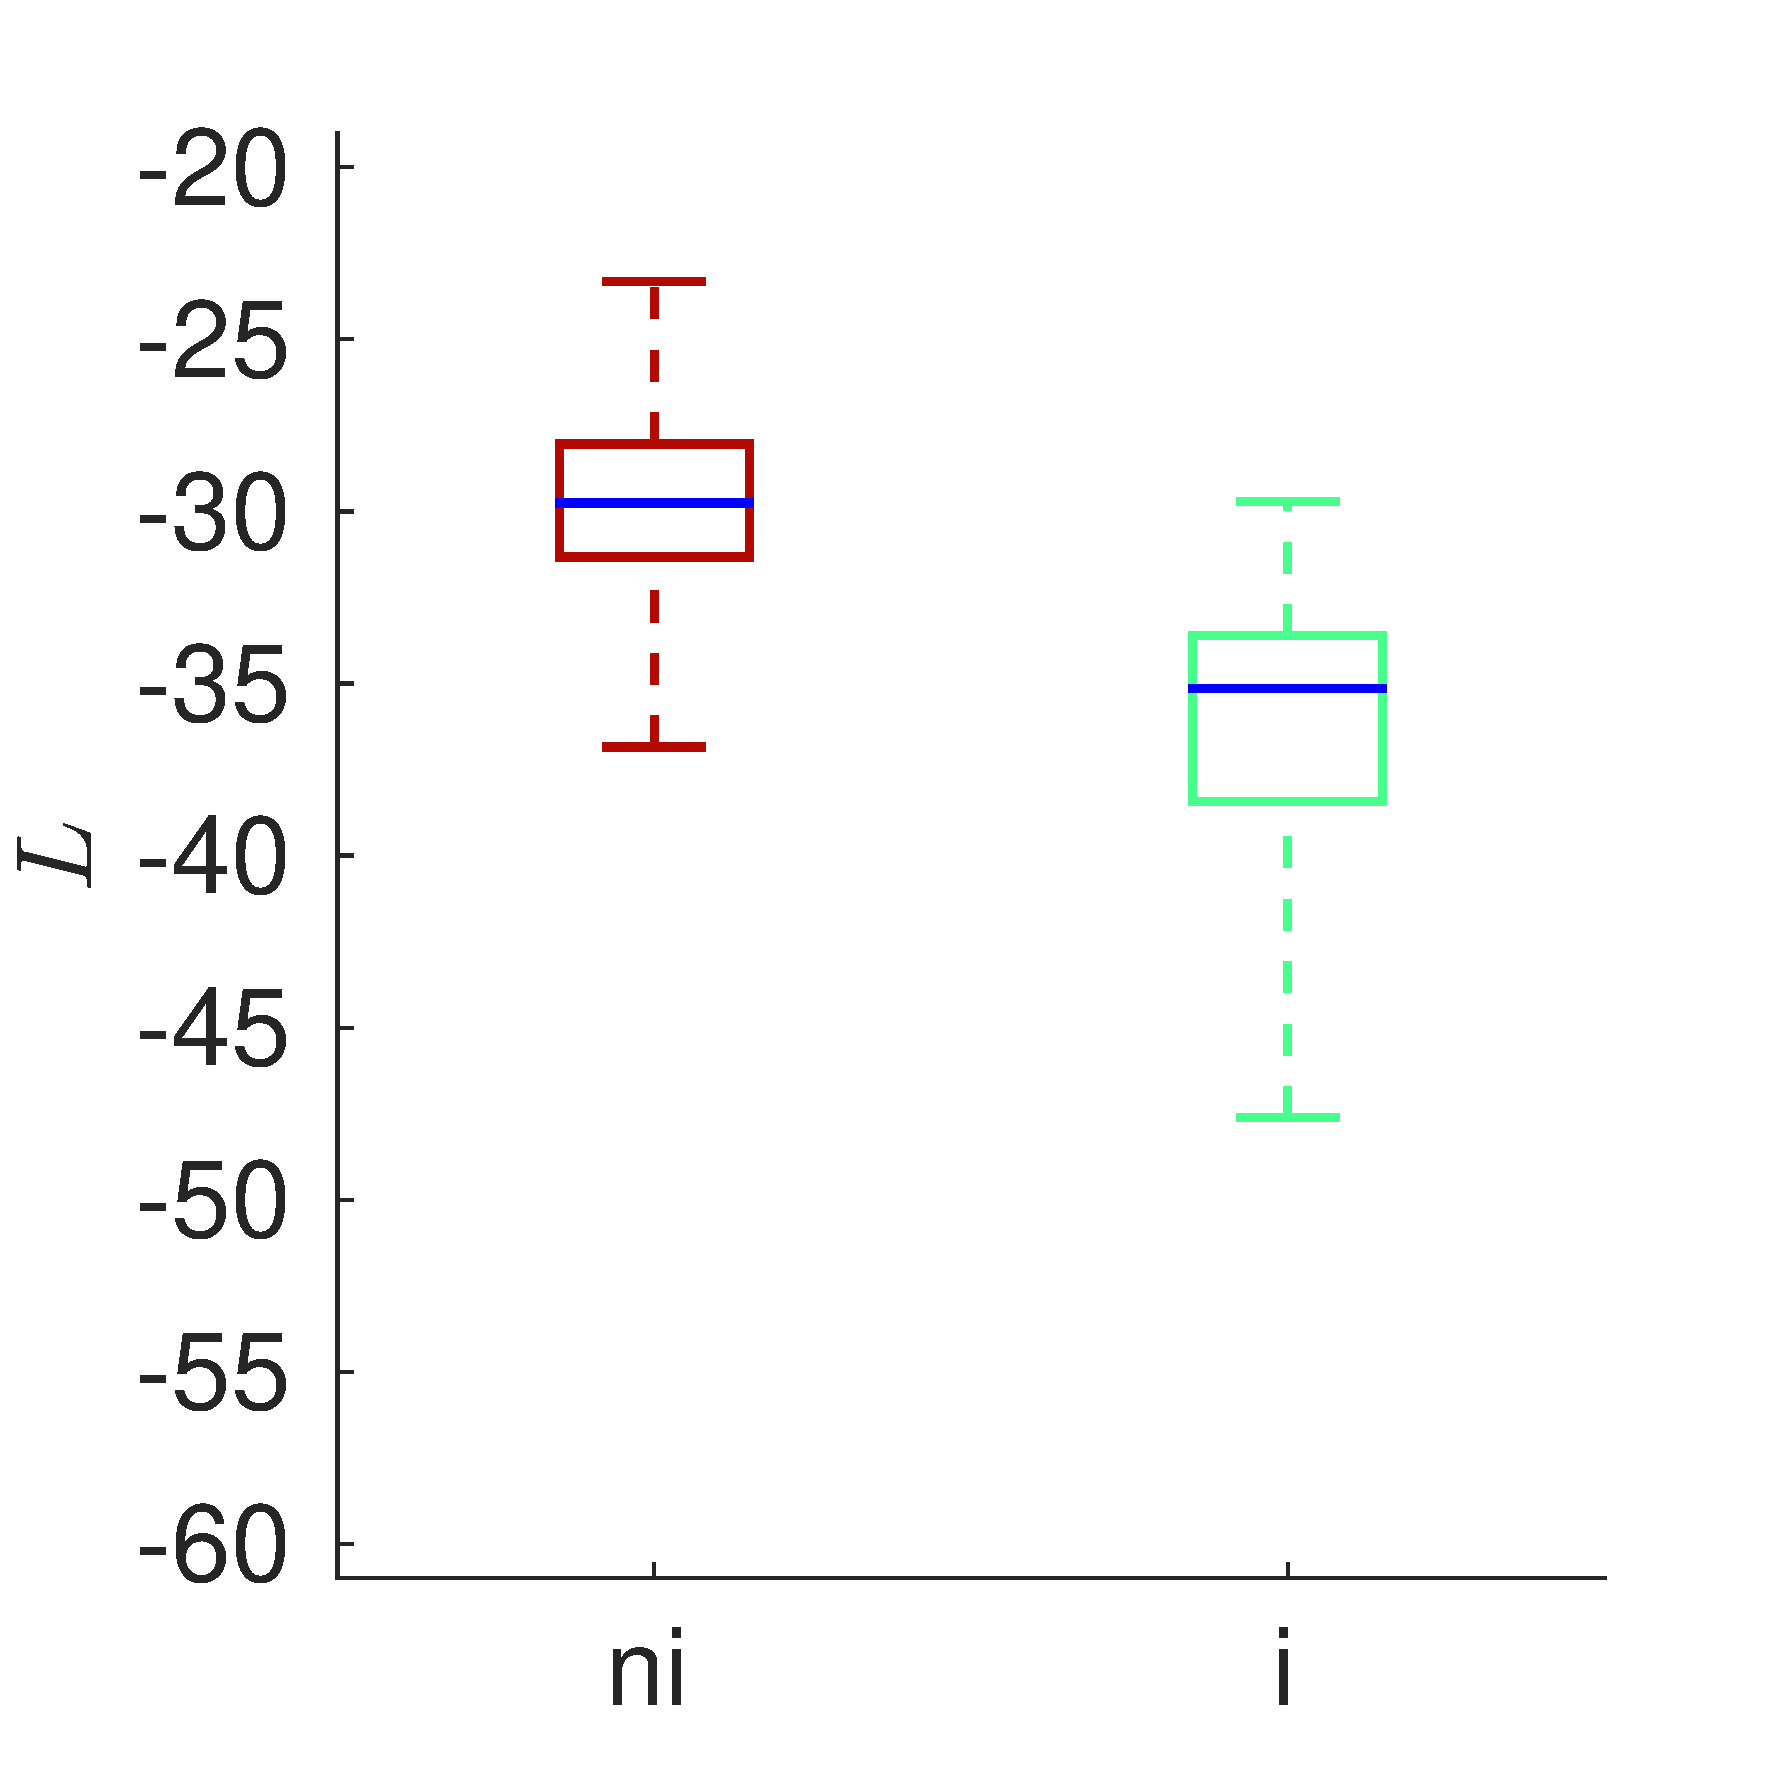
\includegraphics[width=.33\linewidth]{gfx/xp_soundlevel_1}\label{fig:soundlevela}}
        \subfloat[]
        {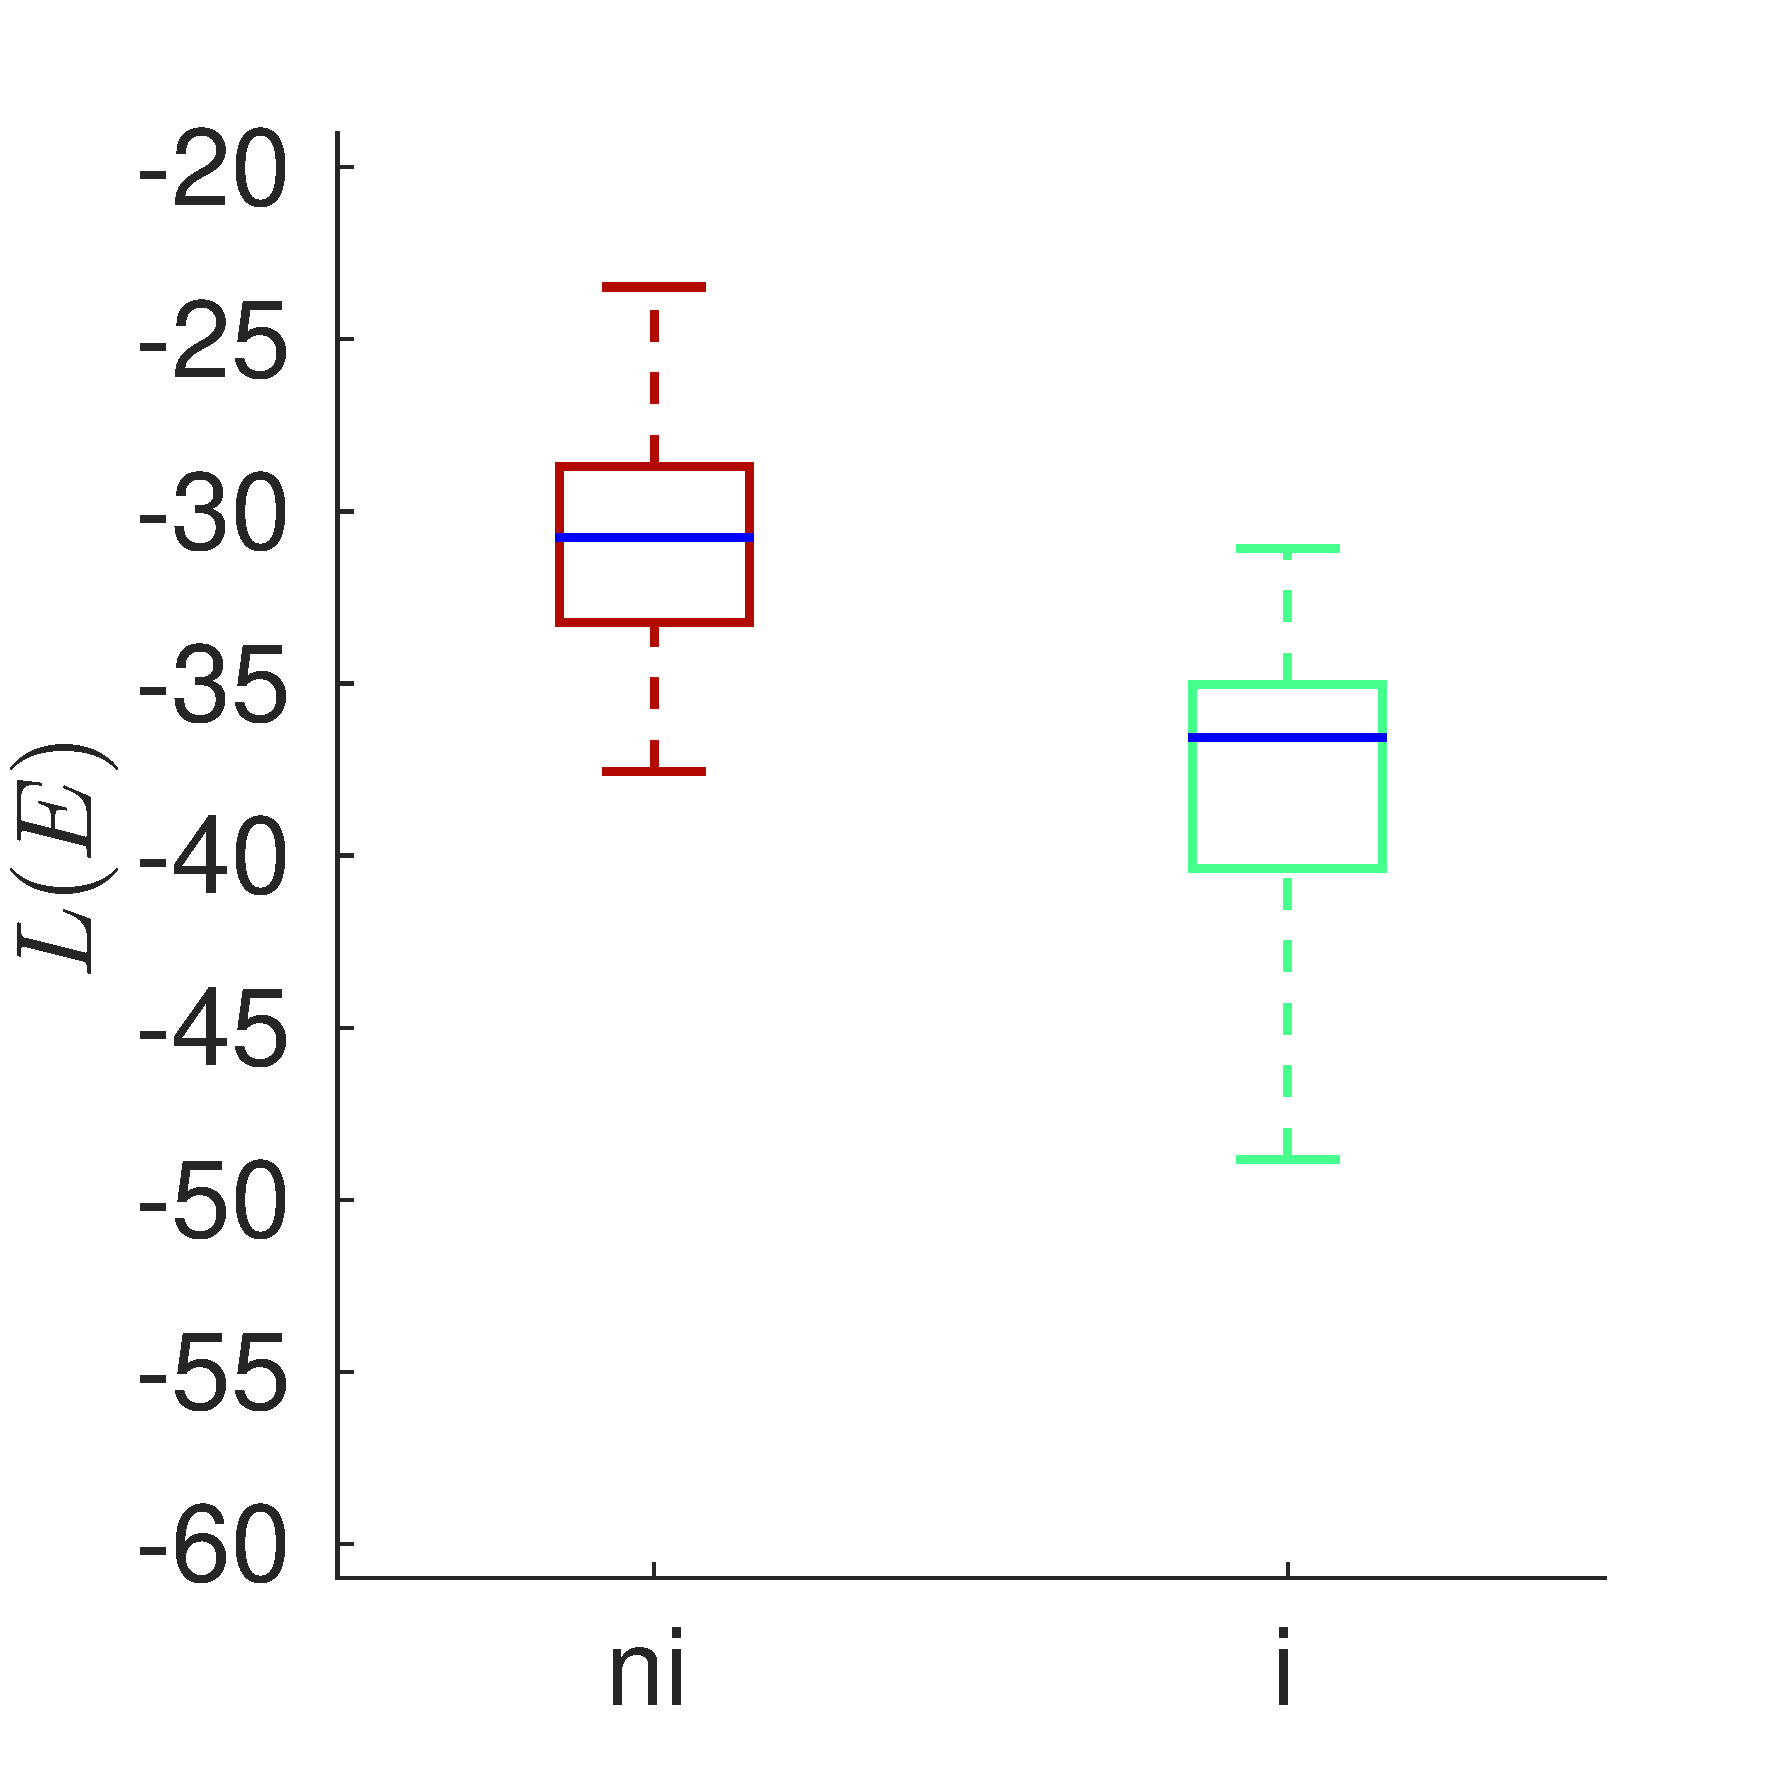
\includegraphics[width=.33\linewidth]{gfx/xp_soundlevel_3}\label{fig:soundlevelb}}
        \subfloat[]
        {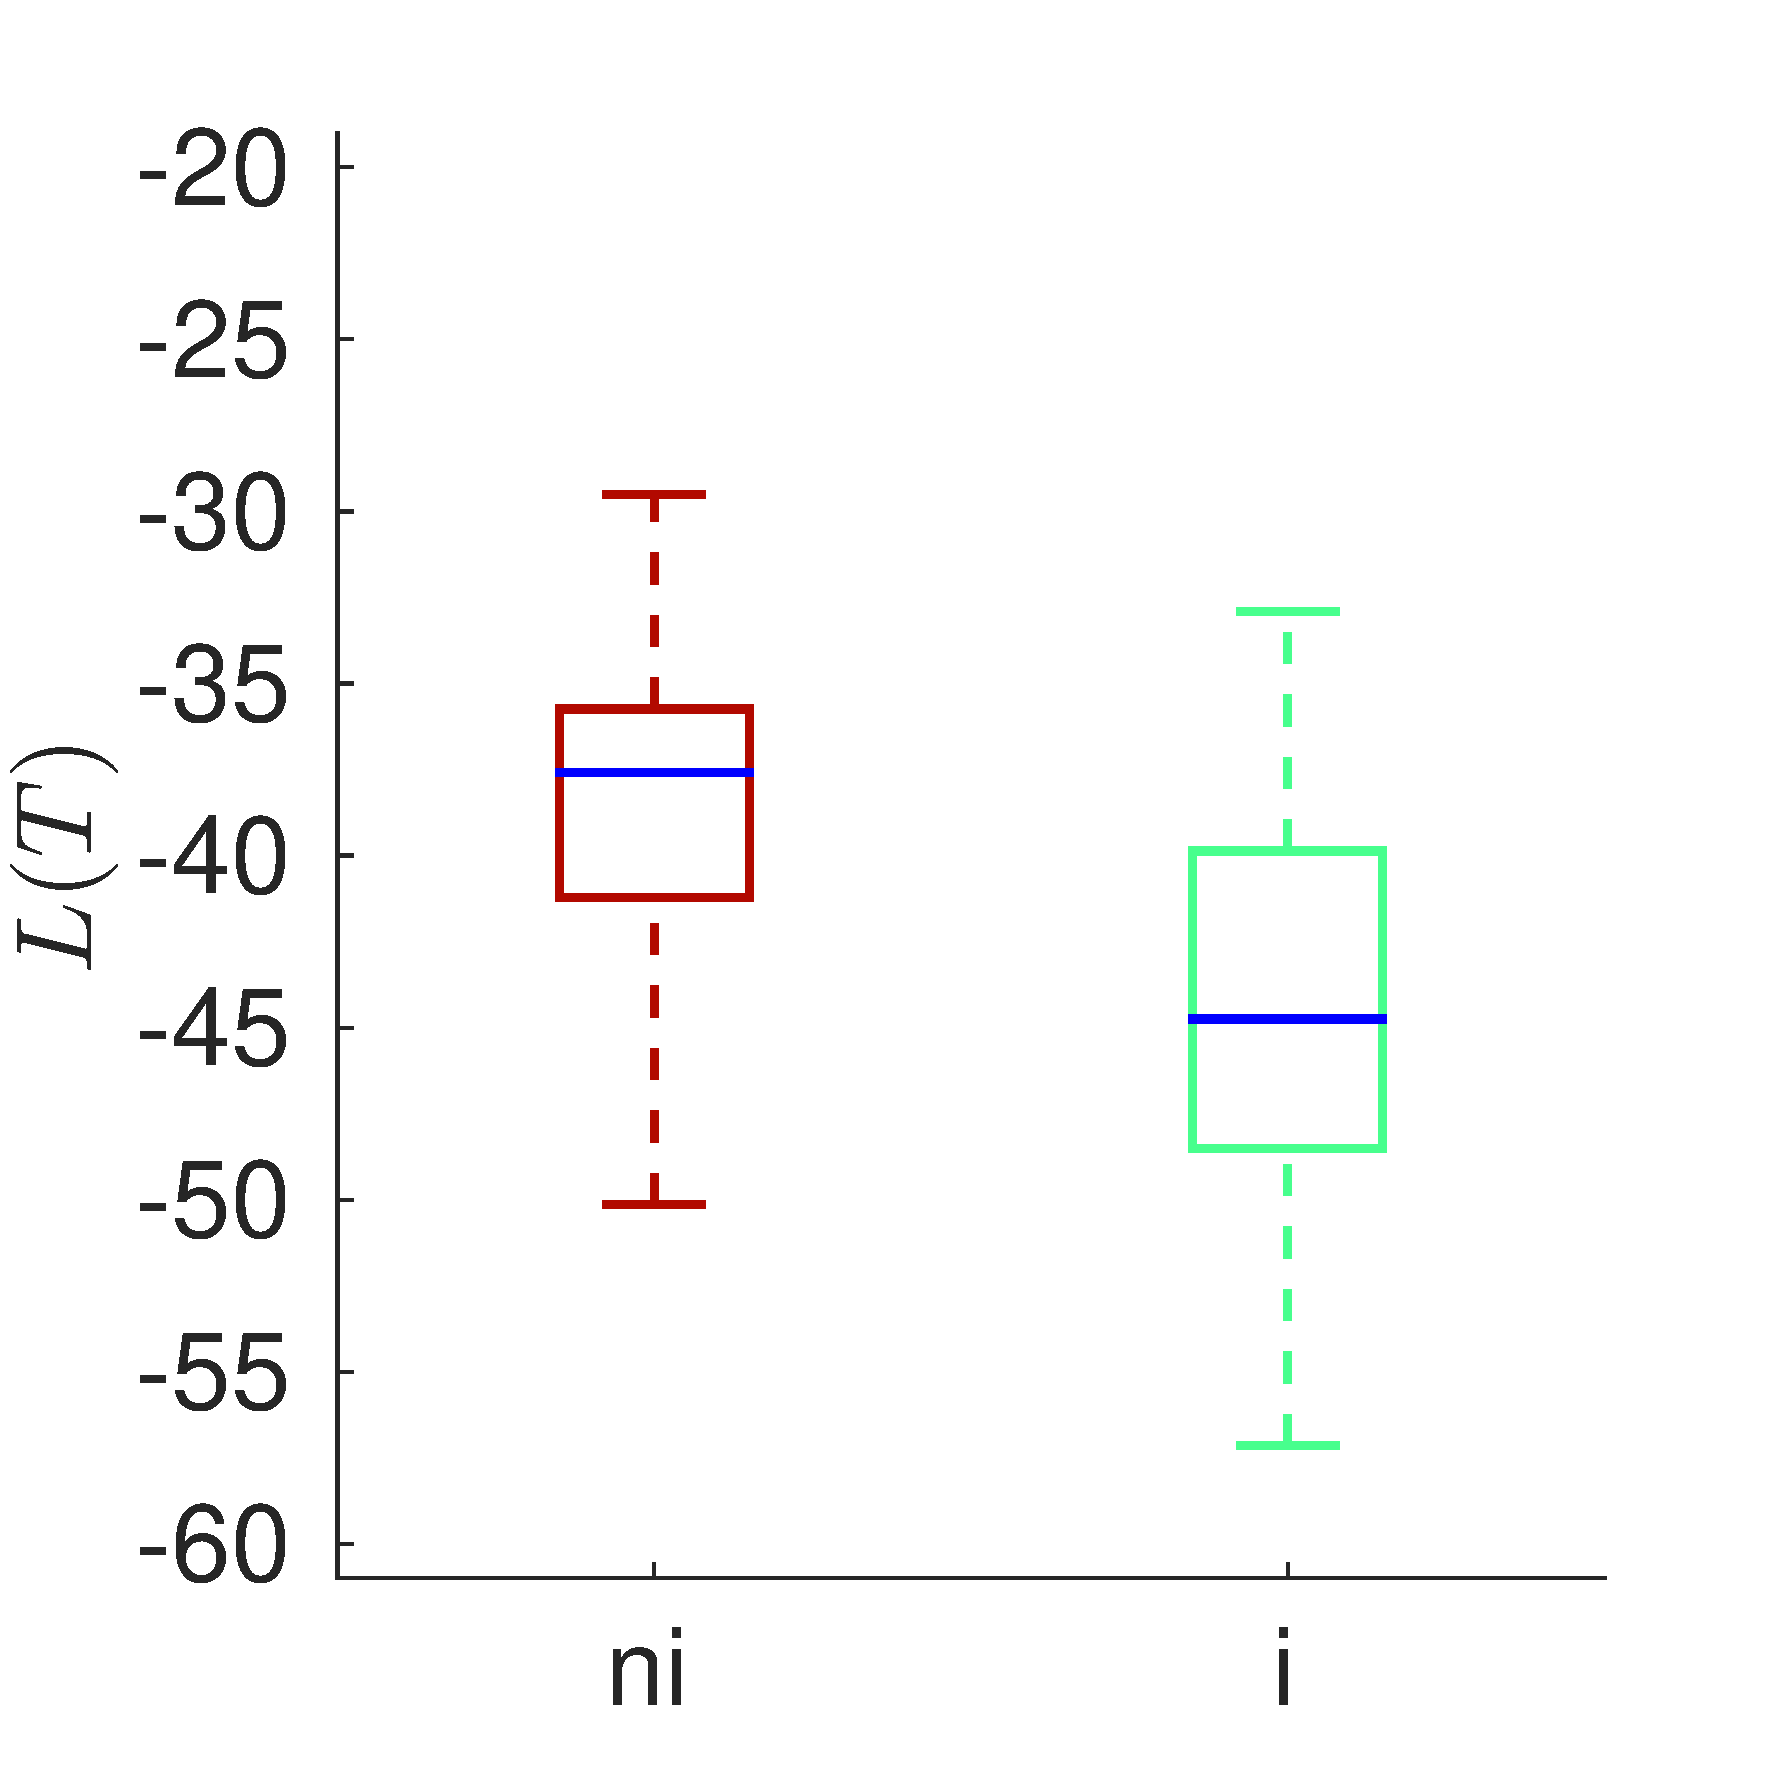
\includegraphics[width=.33\linewidth]{gfx/xp_soundlevel_5}\label{fig:soundlevelc}}\par
        \subfloat[]
        {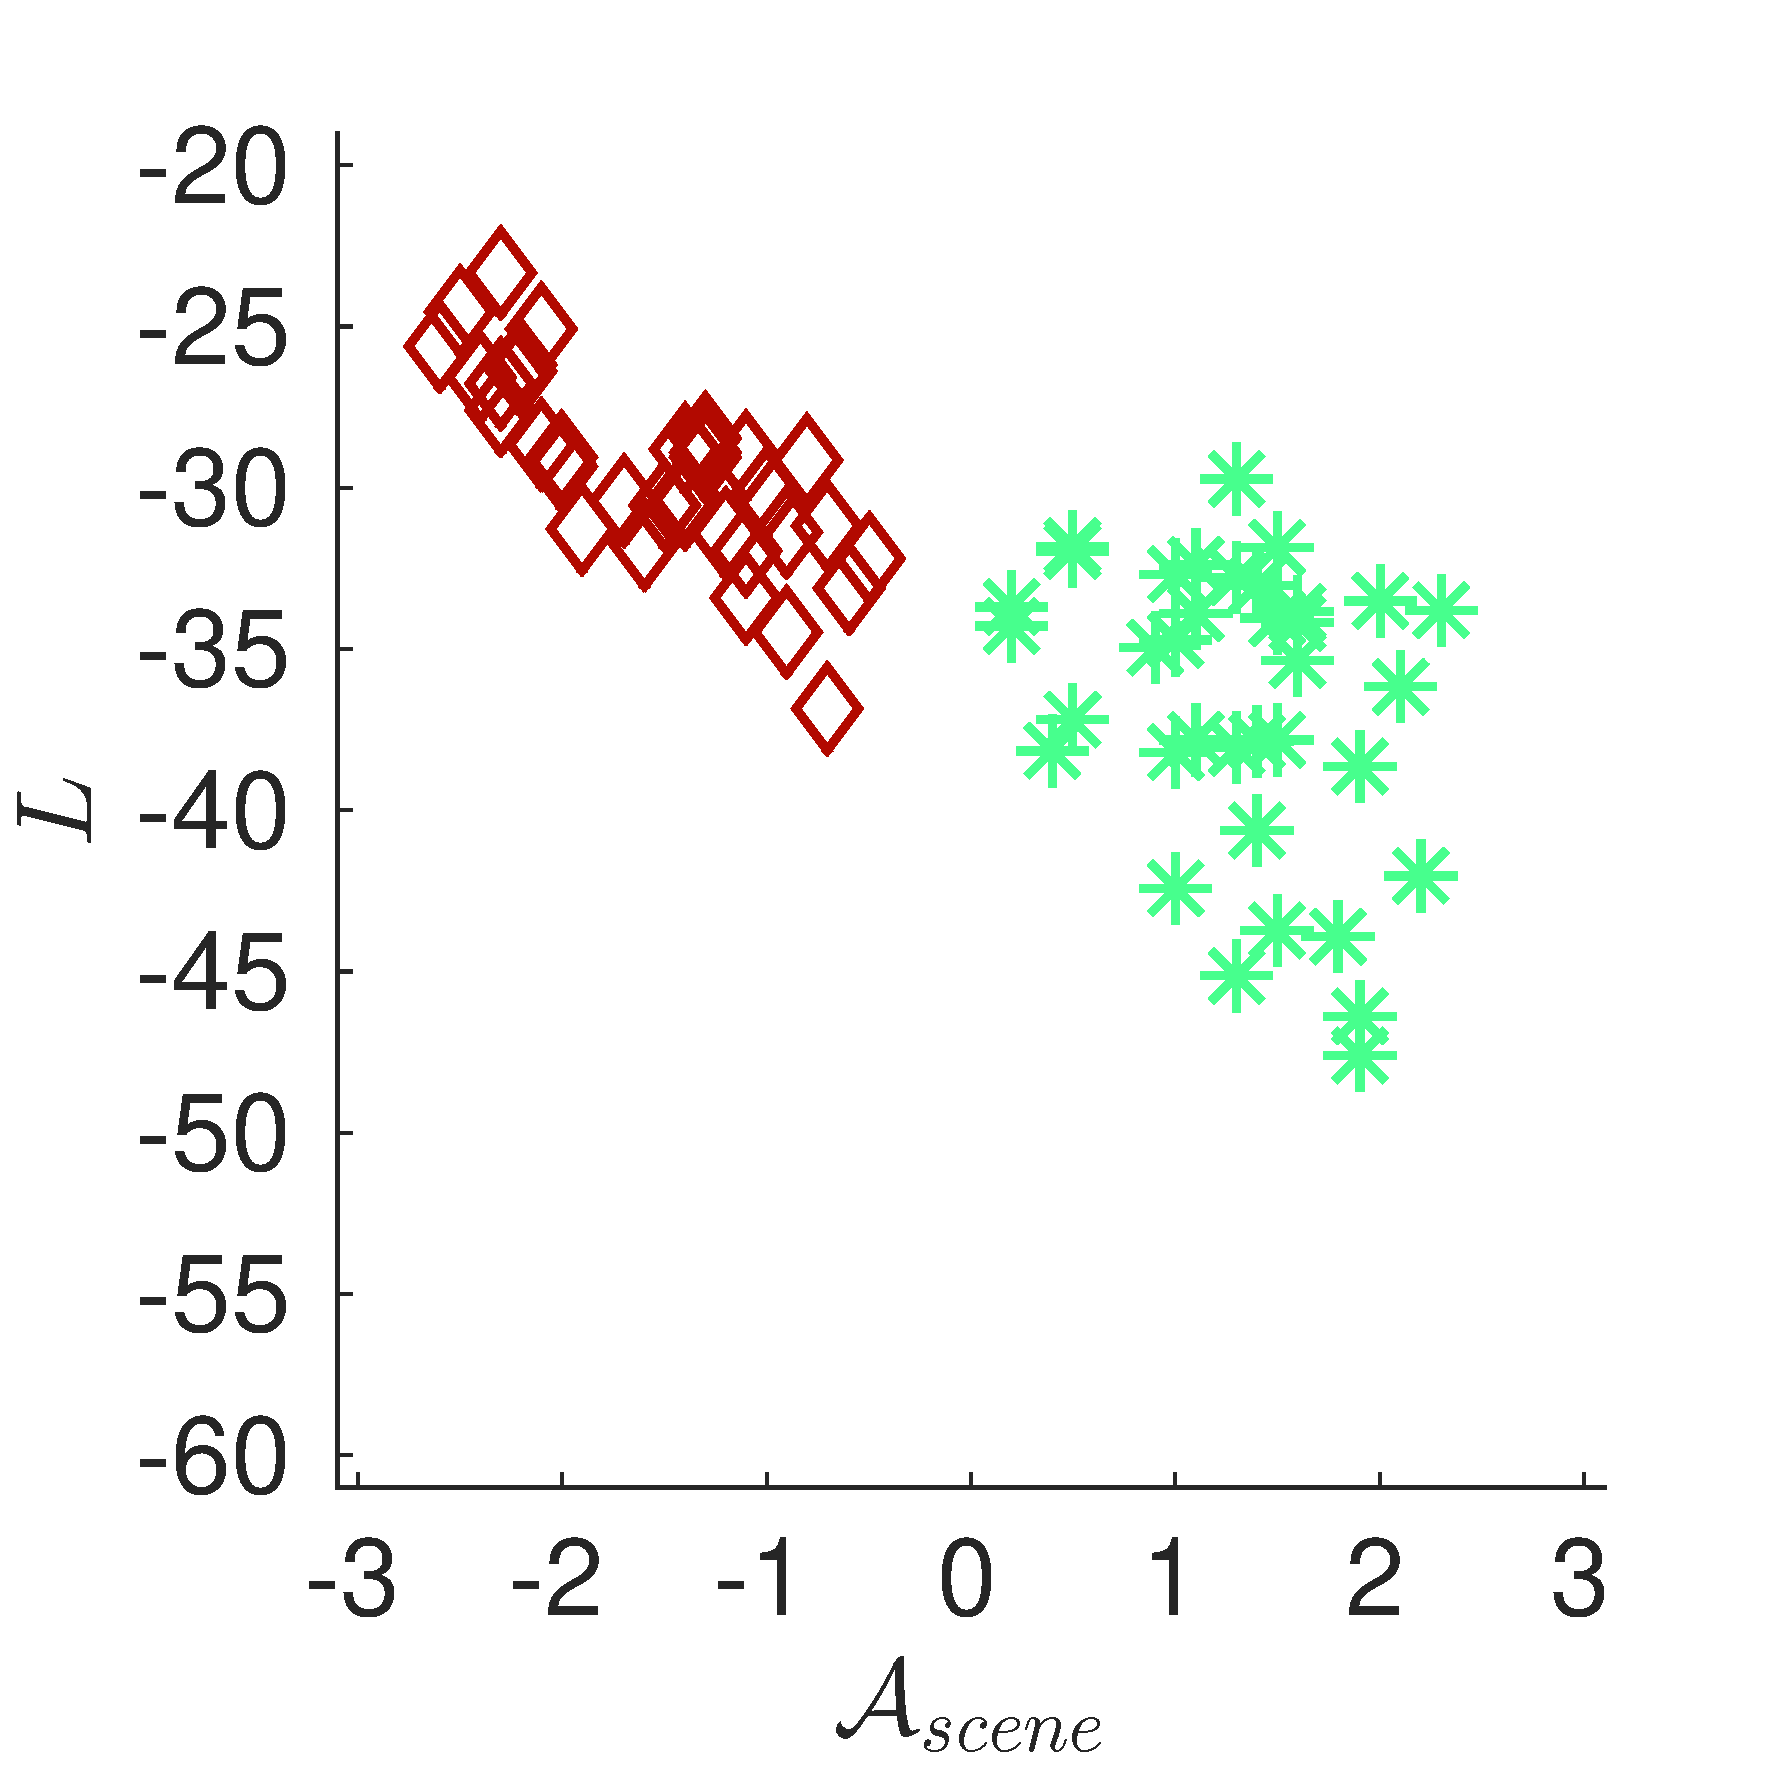
\includegraphics[width=.33\linewidth]{gfx/xp_soundlevel_2}\label{fig:soundleveld}}
        \subfloat[]
        {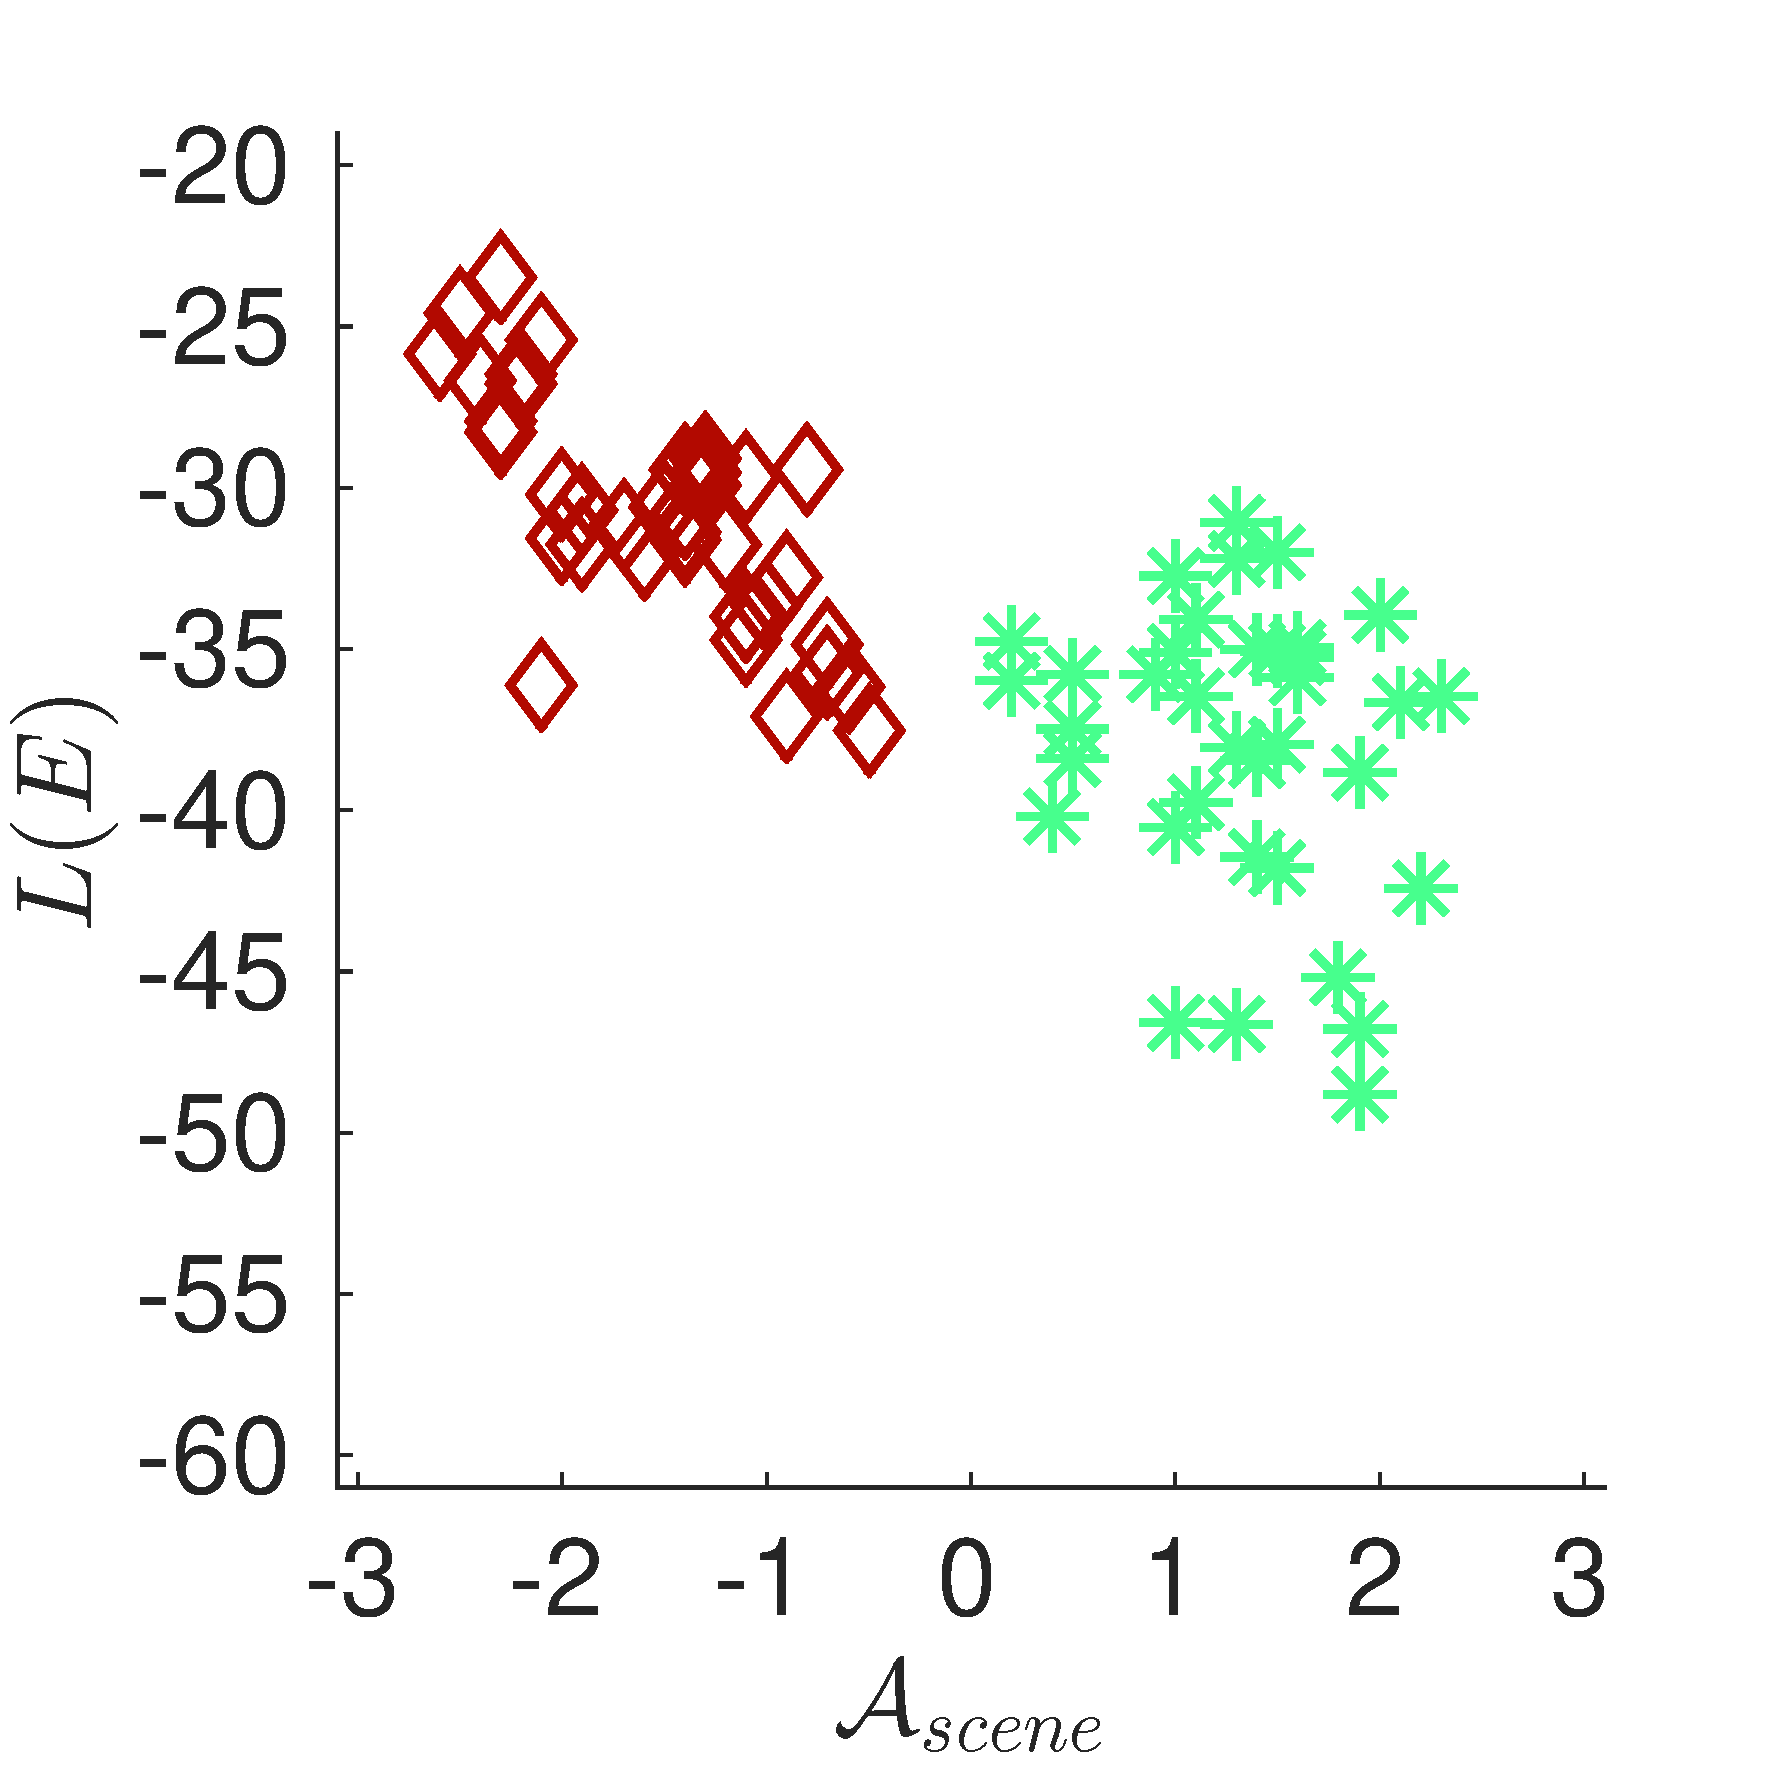
\includegraphics[width=.33\linewidth]{gfx/xp_soundlevel_4}\label{fig:soundlevele}}
        \subfloat[]
        {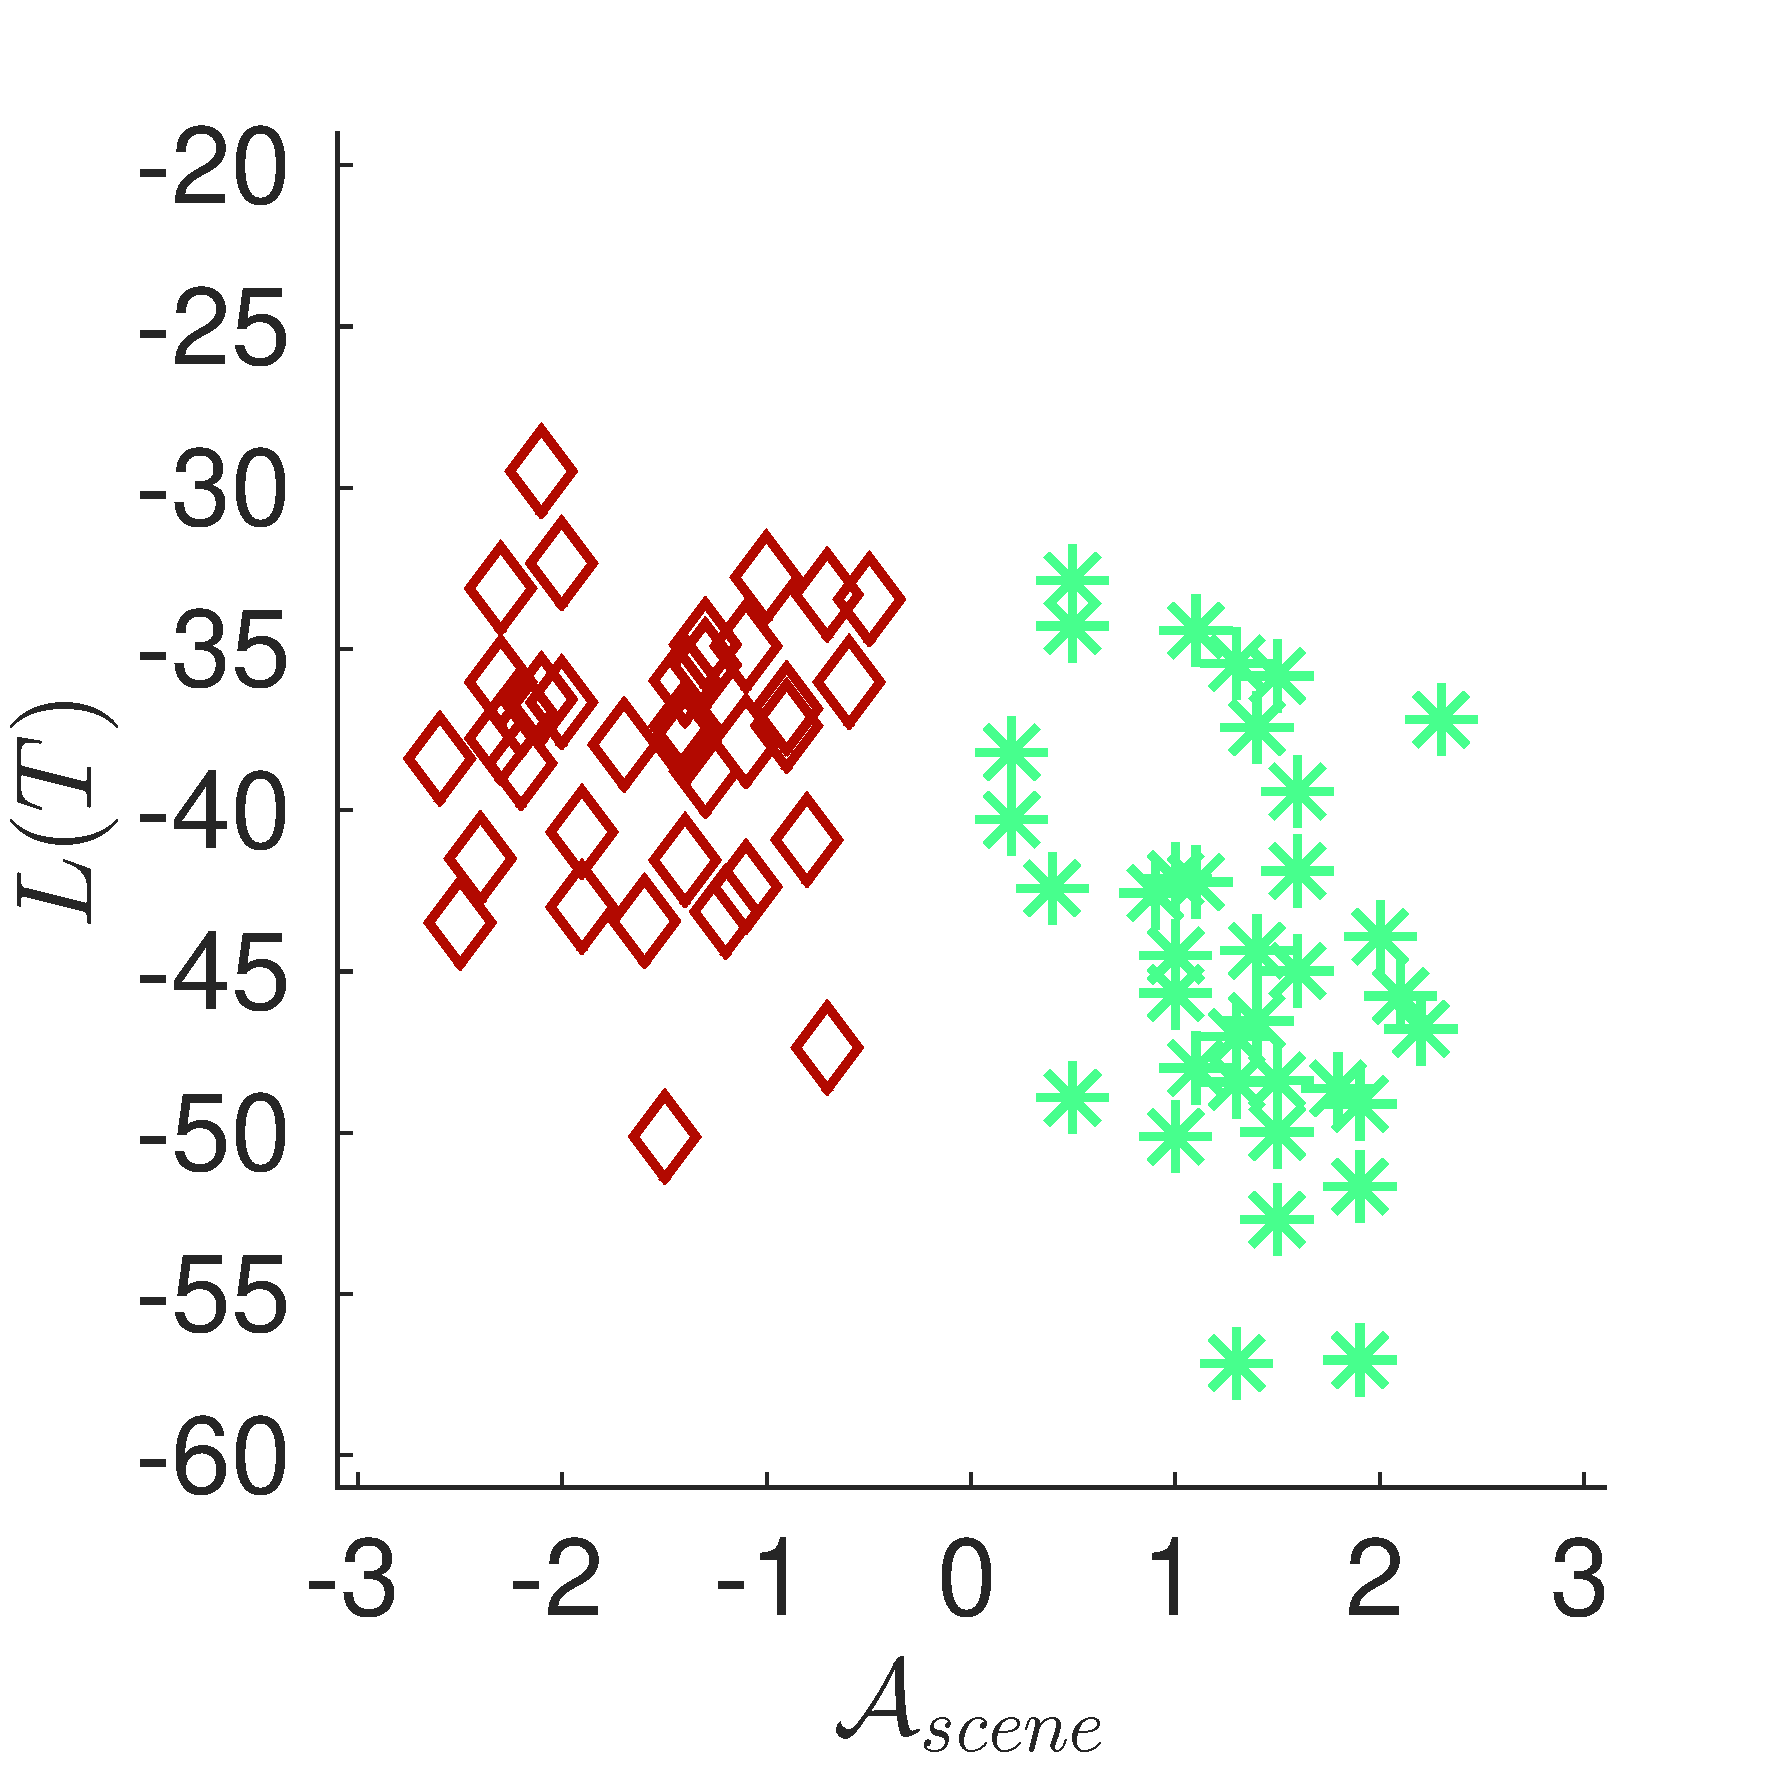
\includegraphics[width=.33\linewidth]{gfx/xp_soundlevel_6}\label{fig:soundlevelf}}
       \caption{Distributions of the sound levels $L$ (a, d), $L(E)$ (b, e) et $L(T)$ (c, f), with respect to scene type (a, b, c) and perceived pleasantness $\mathcal{A}_{scene}$ of experiments 1.b (d, e, f).}
\end{figure}

%En premier lieu, nous nous concentrons sur le niveau sonore. Les figures~\ref{fig:soundlevela},~\ref{fig:soundlevelb} et~\ref{fig:soundlevelc} affichent les distributions des niveaux $L$, $L(E)$ et $L(T)$. Il existe bien une différence de niveau significative entre les i- et ni-scènes ($L$: $p<0.01$), avec un écart des moyennes de -7 $dB$. Cette différence affecte aussi bien les événements ($L(E)$: $p<0.01$, écart moyen: -7 $dB$) que les textures ($L(T)$: $p<0.01$, écart moyen: -6 $dB$).

First, our analyses focuses on the sound levels. Figures ~\ref{fig:soundlevela},~\ref{fig:soundlevelb} and~\ref{fig:soundlevelc} respectively depict the distribution of the levels $L$, $L(E)$ and $L(T)$. There is a significant difference in terms of sound levels between i- and ni-scenes ($L$: $p<0.01$). This difference is significant for events ($L(E)$: $p<0.01$, mean deviation: -7 $dB$) and for textures ($L(T)$: $p<0.01$, mean deviation: -6 $dB$).

%Nous vérifions, sans surprise, que le niveau des sources sonores est bien un indicateur d'agrément, les ni-scènes ayant tendance à être plus fortes, fait rapporté dans un grand nombre d'études. Nous constatons encore que cette différence de niveau s'observe de manière égale pour les événements et les textures sonores.

As expected, the sound level of the sources is indeed a pleasantness indicator, as the ni-scenes tend to be louder. This results is also an outcome of a large number of related works. We also notice that this difference of sound levels is both significant for events or textures.

%Il apparaît que ce sont les événements qui impactent le plus le niveau global des scènes, l'écart entre $L$ et $L(E)$ n'étant que de 1 $dB$ pour les i-scènes et les ni-scènes. Cette observation fait écho aux résultats obtenus par Kuwano~\al~\cite{kuwano_memory_2003}. Au cours de leur expérience, les auteurs demandent à leurs sujets d'évaluer une série d'environnements sonores de manière globale, dans un premier temps, puis d'en évaluer le niveau aux instants où chacun identifie une source sonore. L'étude montre qu'il n'y a pas de différences significatives entre les jugements globaux et les moyennes des jugements instantanés. Pour en revenir à notre expérience, c'est comme si nos sujets avaient inconsciemment tenu compte de cette réalité perceptive lors de la simulation, en faisant porter le niveau sonore global par des sons courts et bien identifiés, \ie~les événements.

It appears that the biggest influence on the global sound levels comes from the events, the difference between $L$ and $L(E)$ being only 1 $dB$ for i- and ni-scenes. This observation is in agreement with the results obtained by Kuwano~\al~\cite{kuwano_memory_2003}. During their experiment, the authors ask their subjects to assess a set of soundscapes at a global level and then to do the same judgment at the time when they detect a sound source. The study shows that there is no significant difference between global and averaged instantaneous judgments. In our case, the result can be interpreted as if the subjects had unconsciously integrated this perceptual reality when composing the scenes, by allocating most of the global sound levels to well identified and relatively short sounds, \ie the events.

%Nous observons, enfin, que le niveau seul ne permet pas de clairement faire la distinction entre les différents types d'environnement. En effet, $20\%$ des i-scènes ont un niveau supérieur au niveau minimal des ni-scènes, alors qu'il n'y a pas de recouvrement, si l'on considère l'agrément perçu $\mathcal{A}_{scene}$.

Though, the level alone is not sufficient to differentiate completely between i- and ni-scenes. In fact, $20\%$ of the i-scenes have a sound levels higher than the nominal level of the ni-scenes, while there is no overlap when considering the perceived pleasantness $\mathcal{A}_{scene}$.

\subsubsection*{Influence of the sound levels on the perceived pleasantness}

\begin{table}[t]
\centering
\begin{tabular}{l c c c}
               & all scenes                & i-scenes          & ni-scenes    \\
\hline
$L$            & \textbf{-0.77} ($p<0.01$) & -0.32 ($p=0.06$)  & \textbf{-0.78} ($p<0.01$)\\
$L(E)$         & \textbf{-0.75} ($p<0.01$) & -0.20 ($p=0.24$)  & \textbf{-0.75} ($p<0.01$)\\
$L(T)$         & \textbf{-0.53} ($p<0.01$) & -0.33 ($p=0.05$)  &  -0.00 ($p=0.99$) \\
\hline
\end{tabular}
\vspace{0.5mm}
\caption{Linear correlation coefficients computed between mean perceived pleasantness $\mathcal{A}_{scene}$ of experiment 1.b and sound levels.}
\label{tab:corrStructA}
\end{table}

%Dans cette partie, nous analysons les relations fines qui peuvent exister entre les descripteurs structurels, d'une part, et l'agrément perçu, d'autre part. Contrairement à la section précédente, où la qualité affective des scènes est représentée de manière binaire (i \vs~ni), nous considérons ici l'agrément moyen $\mathcal{A}_{scene}$ comme descripteur perceptif. Il s'agit d'étudier l'existence de potentielles corrélations entre les descripteurs structurels et $\mathcal{A}_{scene}$. Les coefficients de corrélations linéaires calculés entre $\mathcal{A}_{scene}$ \vs~$L$, $L(E)$, $L(T)$ sont présentés dans le tableau~\ref{tab:corrStructA}. Les relations entre $\mathcal{A}_{scene}$ et les descripteurs structurels sont illustrées par les figures~\ref{fig:soundleveld},~\ref{fig:soundlevele} et ~\ref{fig:soundlevelf}.

In this section, more detailed relationships that could exist between sound levels and perceived pleasantness are investigated. Contrary to the previous section, we do not consider the pleasantness property of a scene on a binary mode (i vs. ni): we consider here the mean pleasantness $\mathcal{A}_{scene}$ as the perceptual feature. The aim is to investigate the level of correlation between sound levels and $\mathcal{A}_{scene}$. The linear correlation coefficients computed between $\mathcal{A}_{scene}$ \vs~$L$, $L(E)$, $L(T)$ are shown on Table~\ref{tab:corrStructA}. Relationships between $\mathcal{A}_{scene}$ and the sound levels are depicted in Figure~\ref{fig:soundleveld},~\ref{fig:soundlevele} and~\ref{fig:soundlevelf}.

%Concernant $L$, on observe une forte corrélation négative ($r=-0.77$, $p<0.01$) avec $\mathcal{A}_{scene}$, indiquant que plus le niveau sonore est élevé, plus la scène est désagréable. Cependant, la figure~\ref{fig:soundleveld} suggère que cette relation ne s'opère pas de la même manière pour les i- et ni-scènes. En effet, la corrélation entre $L$ et $\mathcal{A}_{scene}$, pour les ni-scènes, reste élevée ($r=-0.78$, $p<0.01$), mais est inexistante pour les i-scènes.

Concerning $L$, a strong negative correlation with $\mathcal{A}_{scene}$ is measured ($r=-0.77$, $p<0.01$), indicating that the higher the sound level is, the more unpleasant the scene is perceived. Nevertheless, Figure~\ref{fig:soundleveld} suggests that this relationship do not occur in the same way for i- and ni-scenes. In fact, the correlation between $L$ and $\mathcal{A}_{scene}$, remains high for ni-scenes ($r=-0.78$, $p<0.01$), but is quasi null for i-scenes.

%Ce résultat, considérant l'ensemble des scènes, s'explique par le fait que les i-scènes ont tendance à être moins fortes que les ni-scènes, donnant ainsi l'illusion de prolonger la corrélation négative observée pour les ni-scènes.

When considering the whole set of scenes, the fact that the level is indeed a good indicator of pleasantness can be explained by the fact that the i-scenes tend to be softer than the ni-scenes, thus allowing us to extend artificially to the i-scenes the negative correlation observed for the ni-scenes.

%Nous en concluons que $L$:
%
%\begin{itemize}
%\item permet bien de faire la distinction entre les i- et ni-scènes,
%\item permet de finement caractériser l'agrément perçu des ni-scènes,
%\item n'est pas un indicateur pertinent de l'agrément perçu pour des environnements a priori agréables.
%\end{itemize}

We thus conclude that $L$:

\begin{itemize}
\item allows us to differentiate between i- and ni-scenes,
\item characterizes precisely the perceived pleasantness for ni-scenes,
\item is not a relevant feature for modeling the perceived pleasantness of an \textit{a priori} pleasant soundscape (i-scene).
\end{itemize}

%Les mêmes constats sont faits concernant $L(E)$ (\cf~Figure~\ref{fig:soundlevele}). Pour $L(T)$ (\cf~Figure~\ref{fig:soundlevelf}), la corrélation modérée observée sur les scènes considérées dans leur globalité n'apparaît plus sur les i-scènes et ni-scènes considérées de façon séparée (i-scènes: $r=-0.33$, $p=0.05$, ni-scènes: $r=-0.00$, $p=0.99$). On peut penser que la corrélation négative émergeant au niveau l'ensemble est un artefact résultant du fait que le niveau des textures des i-scènes a tendance à être plus bas que celui des ni-scènes. Ainsi, si les événements sonores conservent une certaine capacité de prédiction de l'agrément pour les ni-scènes, le niveau des textures n'apporte, lui, que peu d'informations, quel que soit l'environnement.

The same conclusions can be drawn for $L(E)$, see~Figure~\ref{fig:soundlevele}. For $L(T)$, as shown on~Figure~\ref{fig:soundlevelf}, the moderate correlation observed for the whole set of scenes disappears when separate scenes are considered (i-scenes: $r=-0.33$, $p=0.05$, ni-scenes: $r=-0.00$, $p=0.99$). Again, we believe that the negative correlation coming from the whole is an artifact due to the level difference between the two types of scenes (i-scenes tend to be softer than ni-scenes). Thus, the sound events keep a relative ability to predict the pleasantness of the ni-scenes, but the level of the textures do not bring a lot of information whatever the type of environment is.

%En résumé, en présence d'un environnement désagréable, les niveaux sonores, en particulier ceux des événements, ont un impact négatif sur l'agrément. En présence d'un environnement agréable, en revanche, aucun des descripteurs structurels considérés ici ne semble influer sur la perception de l'agrément.

To sum up, for an unpleasant environment, sound levels - especially those of the events - negatively influence the perceived pleasantness. On the contrary, for a pleasant environment, none of the sound levels considered in the study seem to influence the perceived pleasantness.

%Ces premiers résultats pourraient montrer qu'il existe deux modes de perception, mobilisant chacun des descripteurs indépendants, modes qui s'activent en fonction de la nature de l'environnement (i ou ni).
%
%Le fait que $L$ ne permet pas de caractériser l'agrément des i-scènes peut nous amener à penser que toutes les sources sonores ne contribuent pas de manière égale à la perception de l'agrément, mais que seules le niveau de certaines d'entre elles a une réelle influence. Afin d'approfondir ce point, nous analysons, dans la section suivante, les scènes d'un point de vue sémantique, \ie~en nous intéressant à la nature des sources qui les composent.

Those first outcomes tend to show that 1) two modes of perception exist depending on the very nature of the environment (i- or ni-), and 2) each involves independent features. The fact that $L$ is not sufficient to characterize the pleasantness of the i-scenes can lead us to conclude that all the sound sources do not equally contribute to the perception of pleasantness. Thus, we think that only the level of some of them can influence this percept. In order to investigate further in that direction, we analyze in the next section the scenes on a semantic point of view, \ie we take an interest in the nature of the sources they are made of.

\subsubsection*{Analysis of the semantic features}

\begin{figure}[!tp]
		\myfloatalign
        \subfloat[]
        {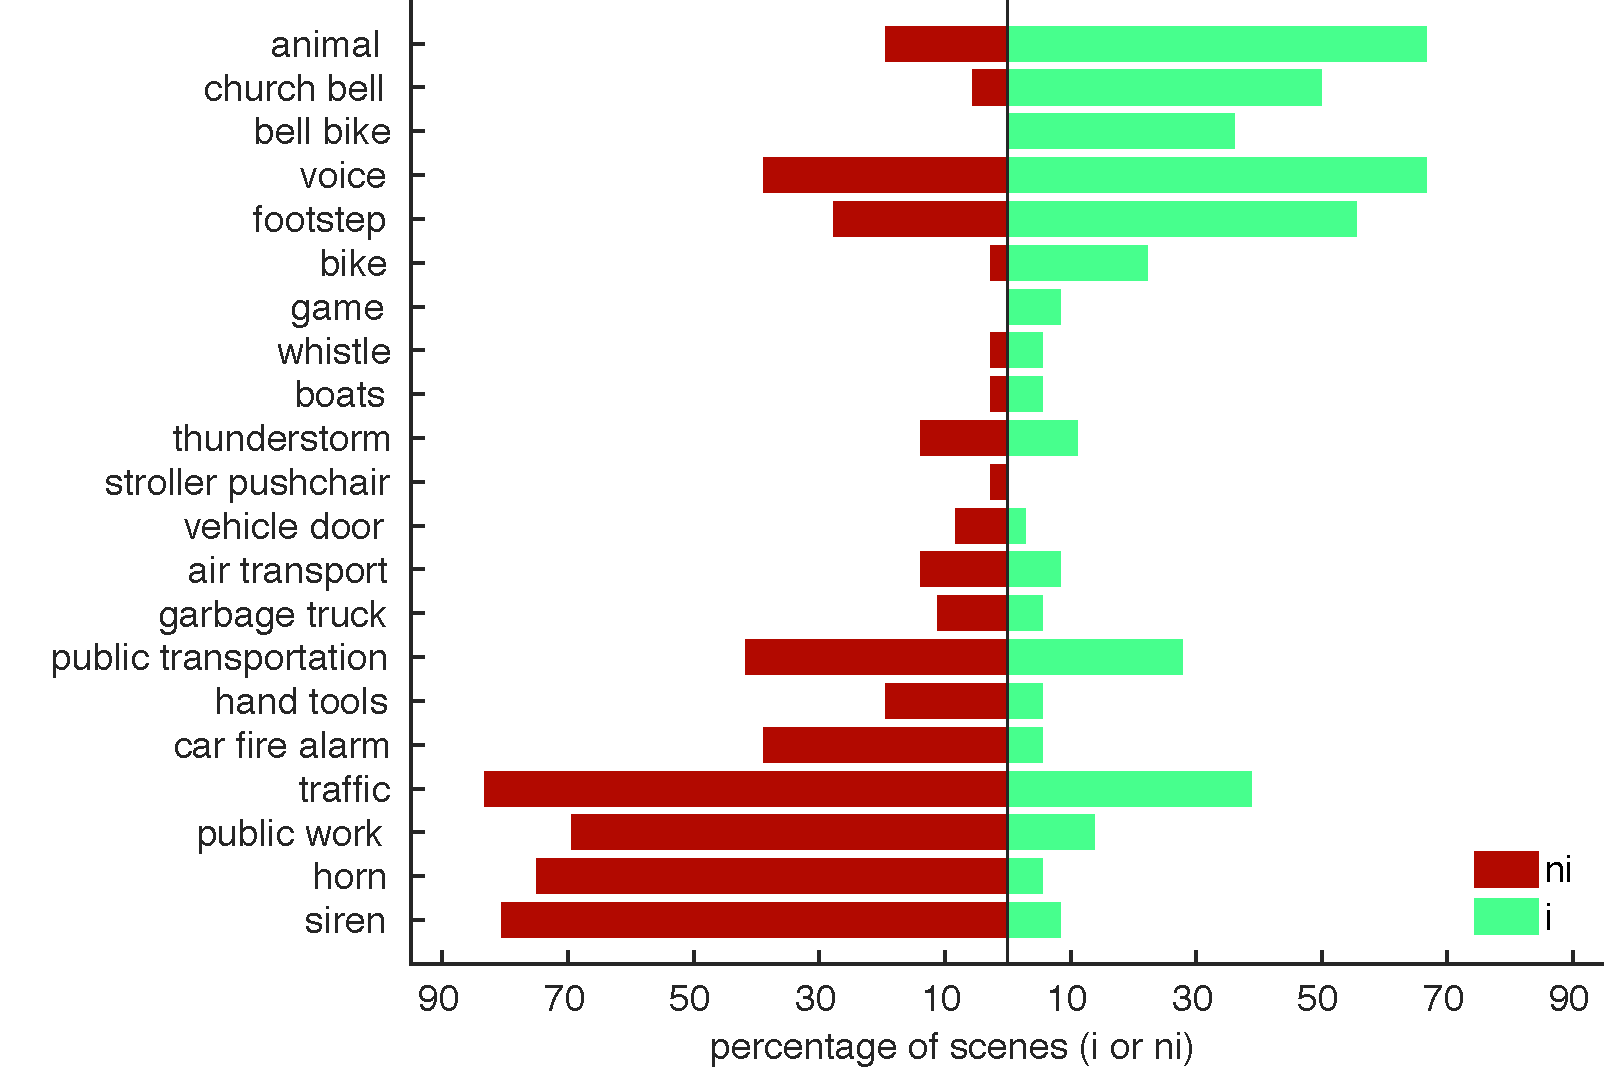
\includegraphics[width=1\linewidth]{gfx/xp1_class_1}\label{fig:soundsourcea}}\par
        \subfloat[]
        {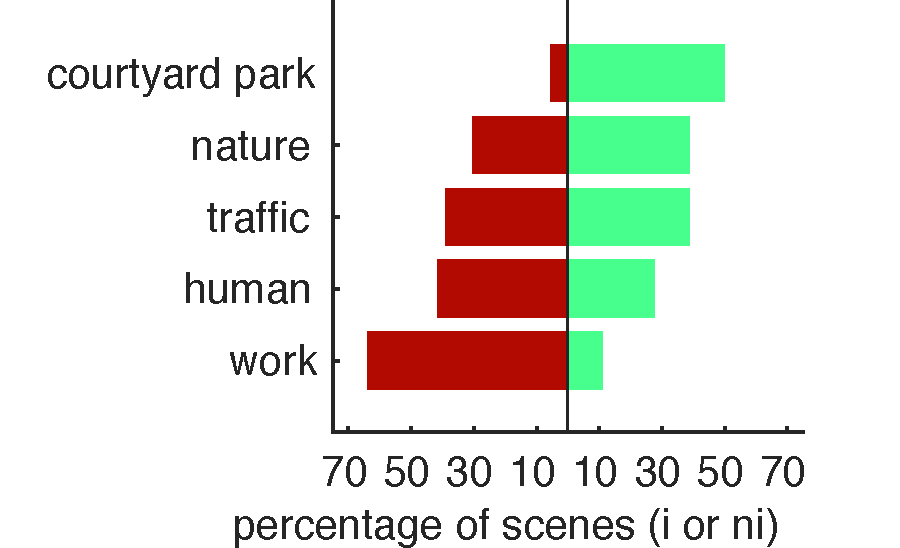
\includegraphics[width=.5\linewidth]{gfx/xp1_class_2}\label{fig:soundsourceb}}
        \subfloat[]
        {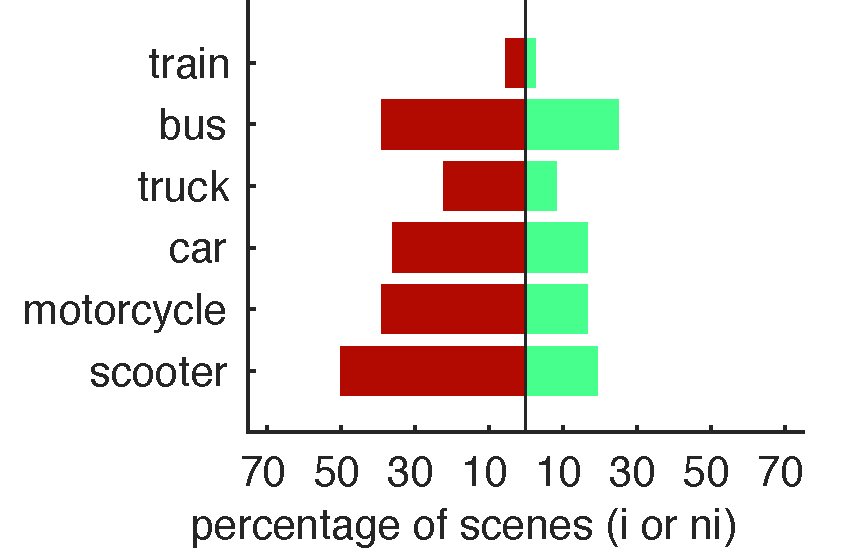
\includegraphics[width=.5\linewidth]{gfx/xp1_class_3}\label{fig:soundsourcec}}
       \caption{Proportion of simulated scenes (i or ni) involving a specific class of sounds: (a) event classes at an abstraction level $0+$, (b) texture classes at an abstraction level $0$, (c) event sub-classes at an abstraction level $1$ belonging to \emph{traffic} and \emph{public transportation} classes of the abstraction level $0$.\gl{TODO : align}}\label{fig:soundsource}
\end{figure}

%Nous analysons la composition des scènes en comptant le nombre de sujets ayant utilisé une classe de sons pour simuler un type d'environnement. Les résultats sont présentés à la figure~\ref{fig:soundsourcea} pour les événements, et à la figure~\ref{fig:soundsourceb} pour les textures. Par souci d'espace, nous choisissons un niveau d'abstraction intermédiaire entre les niveaux 0 et 1, noté $0+$, pour représenter les classes (\cf~Figure~\ref{fig:taxonomie}).

We study the composition of the scenes by counting the number of subjects who used a given class of sounds to simulate the environment. Results are shown on Figure~\ref{fig:soundsourcea} for events and on Figure~\ref{fig:soundsourceb} for textures. For the sake of clarity, a transitional level of abstraction between level 0 and 1, named $0+$ is used to depict classes, see ~Figures~\ref{fig:taxonomieEa}, \ref{fig:taxonomieEb} and \ref{fig:taxonomieT}.

%Nous observons une différence notable dans le choix des classes entre les i- et ni-scènes. La répartition des classes est très proche de celle obtenue dans une étude similaire sur les environnements sonores urbains idéaux \cite{guastavino2006ideal}, \ie~les classes suggérant la présence humaine et la nature sont très présentes dans les i-scènes, a contrario, les classes désignant des sons mécaniques et/ou de travaux sont principalement utilisées pour les ni-scènes.

We observe a noticable difference in terms of class choices between the i- and ni-scenes. The distribution of the classes is very similar to the one obtained in a related work on ideal urban soundscapes \cite{guastavino2006ideal}, \ie~ on one hand, classes involving human presence and nature are prevailing in the i-scenes, and on the other hand, classes involving mechanical sounds and/or public works are prevailing in the ni-scenes. These results confirm a previously observed fact: the semantic nature of the sound sources play an important role in the assessment of the environment \cite{raimbault2005urban,dubois2006cognitive}.

%Dans une certaine mesure, nos résultats contredisent ce fait. La figure~\ref{fig:soundsourcea} montre, en effet, que les classes d'événements de \emph{transports publics} (\emph{bus} et \emph{train}, \cf~Figure~\ref{fig:soundsourcec}) ont été utilisées par les sujets, pour des i-scènes, dans $28\%$ des cas, et pour des ni-scènes, dans $42\%$ des cas. Les résultats ne remettent pas en question le fait que les sons de \emph{transports publics} soient bien acceptés: $25\%$ des sujets ont utilisé la classe \emph{bus} pour les i-scènes, un chiffre comparable à celui de la classe \emph{Vélo}, et bien supérieur à celui de toute autre classe de véhicules privés. Cependant les classes \emph{transports publics} sont également bien présentes dans les ni-scènes, plus que les classes \emph{voiture} ou \emph{camion} par exemple. La classe \emph{transports publics} ne peut donc pas être considérée comme typique d'un environnement sonore urbain idéal.

Nevertheless, we notice some differences with \cite{guastavino2006ideal}: Guastavino’s results show that sounds of \emph{public transportation} are specific of ideal urban soundscapes. The authors interpret this by the fact that the perception of pleasantness is, among other things, due to socio-cultural factors. Thus, in our representation of the world, sounds of public transportation are positively connoted and tend to be more accepted than sounds of personal vehicles.

To a certain extent, our results contradict this result. In fact,  Figure~\ref{fig:soundsourcea} show that \emph{public transportation} classes (\emph{bus} and \emph{train}, \cf~Figure~\ref{fig:soundsourcec}) have been used by the subjects for $28\%$ of the i-scenes, and for $42\%$ of the ni-scenes. Those results do not state the fact that sounds of \emph{public transportation} are well accepted: $25\%$ of the subjects used \emph{bus} for the i-scenes, a level that is comparable to the \emph{bike} class, and much higher than all the personal vehicles classes. Though, \emph{public transport} classes are also strongly present in the ni-scenes, for instance more than \emph{light vehicle} or \emph{trucks} classes. On the basis of our results, the public transportation class cannot be considered as typical of an ideal urban soundscape.

%Cette différence peut s'expliquer par la nature des deux protocoles expérimentaux utilisés. Comme nous l'avons fait, Guastavino demande à ses sujets de décrire un environnement. Mais ces derniers travaillent de mémoire, alors que nos propres sujets disposent de supports sonores. Le fait que nos sujets soient confrontés à la réalité acoustique des sons, pour recréer leurs environnements, peut avoir pour effet de diminuer l'impact du contexte socio-culturel. D'autres études utilisant des sons comme stimuli montrent que la classe \emph{bus} peut avoir un effet négatif sur l'appréciation de l'environnement \cite{lavandier2006contribution}.

This difference may be explained by the nature of the experimental protocol used in the two studies. As in our study, Guastavino asks the subjects to describe an environment. She asks them to perform this task starting only from their memories whereas, in our case, subjects perform the same task using actual sound samples that they can listen to. The fact that subjects in our experiment are faced to the acoustic reality of the sounds for composing the environment may have decreased the socio-cultural impact. Other studies that considered sounds as stimuli have shown that the \emph{bus} class can have a negative influence on the assessment of the environment \cite{lavandier2006contribution}.

\subsubsection*{Sound markers}

\begin{table}[t]
 \setlength{\tabcolsep}{0.2pt}
 \centering
  {\renewcommand{\arraystretch}{0.9}
\begin{tabular}{c c c c}
Abstraction        & \multicolumn{2}{c}{Event sound markers} \\
level & i-scenes & ni-scenes \\
\hline
0  &                          & construction work (3.78)  \\
\hline
  & church bell  (4.5)             & car horn  (3.9) \\
1 & bicycle bell  (4.3)      & siren (3.9)\\
  & animal (4.2)              &       \\
   \hline
  & bird        (4.8)       & car horn  (4.0)\\
2 & church bell  (4.4)             & siren (4.0)\\
  & bicycle bell     (4.2)             &       \\
   \hline
  & bird song (4.8)        & klaxon  (4.1)\\
3 & church bell   (4.3)            & siren (4.0)\\
  & bicycle bell      (4.2)   &       \\
  & foot steps  (3.6)      &  \\
  &                           & \\
  & \multicolumn{2}{c}{Texture sound markers}      \\
  & i-scenes & ni-scenes \\
\hline
0 &     courtyard / park (4.1) &  construction (3.9)  \\
\hline
1 &     park (3.65)          &  crossroad (3.6)  \\
  &                          &  construction vehicule (3.3)  \\
\hline
2 &     park (3.64)          &  crossroad (3.56)  \\
\hline
\end{tabular}
}
\vspace{0.5mm}
\caption{Event and texture classes identified as sound markers. In each cell, markers are ranked as decreasing order of V-test value. $p\leq0.01$ for all sound markers.}
\label{tab:markers}
\end{table}

%Nous avons mis en évidence que, qualitativement, la composition des sources sonores des scènes diffère selon les types d'environnement (i ou ni). Nous essayons de voir maintenant si, parmi ces classes, certaines sont typiques d'un environnement en particulier. Pour ce faire, nous utilisons le V-test (\cf~Section~\ref{sec:xp1_dataAna}), en considérant séparément chaque niveau d'abstraction. Les résultats sont présentés dans le tableau~\ref{tab:markers}.

We have shown that, on a qualitative point of view, the composition of the scenes in terms of sound sources differs i- or ni-scenes. We now investigate whether some of the sound classes are specific to a given environment. For that purpose, the V-test detailed in  Section~\ref{sec:xp1_dataAna} is considered separately for each abstraction level. Results are presented in Table~\ref{tab:markers}.

%Concernant les événements sonores, 9 marqueurs sont identifiés sur l'ensemble des niveaux d'abstraction. Comme la figure~\ref{fig:soundsource} le laissait présager, les classes relatives à la présence humaine (\emph{pas homme béton}, \emph{sonnette vélo}), et à la nature (\emph{animaux, oiseaux}, \emph{chants d'oiseaux}) sont des marqueurs de i-scènes. Nous notons également la présence de la classe \emph{cloche} dans les marqueurs d'un environnement idéal. Ce fait est possiblement dû au \emph{background} socio-culturel des sujets, dans leur grande majorité, des citoyens européens. En effet, selon Schafer, un son reconnu par un individu comme faisant partie intégrante de son environnement est bien accepté. Les marqueurs de ni-scènes sont des classes faisant référence à des sons de travaux (\emph{travaux}), ou suggérant un trafic dense (\emph{klaxon}, \emph{sirène}).

Regarding the sound events, 9 markers are identified for all abstraction levels. As shown on Figure~\ref{fig:soundsource}, classes related to human presence (\emph{male footsteps on concrete}, \emph{bicycle bell}), and of nature (\emph{animals, bird}, and \emph{bird song}) are i-scenes markers as well as the \emph{church bell} class. This latter result may be due to the socio-cultural background of the subjects who are mostly European citizens. In fact, according to Schafer, a sound that is identified by a person as being an important element of his/her environment, is well accepted. Sound markers of ni-scenes are classes related to construction site (\emph{construction works}), or suggesting a strong traffic (\emph{horn}, \emph{siren}).

%Concernant les textures sonores, 5 marqueurs sont identifiés. Pour les i-scènes, il s'agit de classes faisant référence à des ambiances amorphes, calmes, (\emph{cour-intérieur} et \emph{parc}). Pour les ni-scènes, il s'agit, comme pour les événements, de classes faisant référence à des bruits de travaux (\emph{travaux} et \emph{véhicule de travaux}), ainsi que d'une classe faisant référence au trafic (\emph{carrefour}).

Regarding the textures, 5 markers are identified. For the i-scenes, those classes related to passive or quiet ambiances (\emph{courtyard}, \emph{park}). The marker classes for the ni-scenes are, as for the events, related to construction site (\emph{construction}, \emph{construction vehicle}), together with a class related to traffic (\emph{crossroad}).

%Bien que l'ensemble des marqueurs identifiés soient intuitifs, aucune des classes d'événements faisant directement référence aux bruits de véhicules motorisés n'est un marqueur, exception faite de la classe de textures \emph{carrefour}. Pour représenter un trafic désagréable, les sujets ont porté leurs choix sur les classes \emph{klaxon} et \emph{sirène}. On peut supposer que les sons isolés de véhicules sont compris comme faisant partie intégrante de l'environnement urbain, et ne sont donc pas particulièrement associés à un environnement désagréable.

Although the whole set of identified markers are rather intuitive, none of the event classes related to the noise of the motor vehicles are identified as markers, except for the texture class \emph{crossroad}. To generate an unpleasant traffic, subjects chose the classes \emph{horn} or \emph{siren}. We thus conclude that isolated motor vehicle sounds are understood as being part of the urban environment, and thus their nature is not necessarily linked to an unpleasant soundscape.

\subsubsection*{Representation space induced by semantic features}

\begin{figure}[t]
        \myfloatalign
        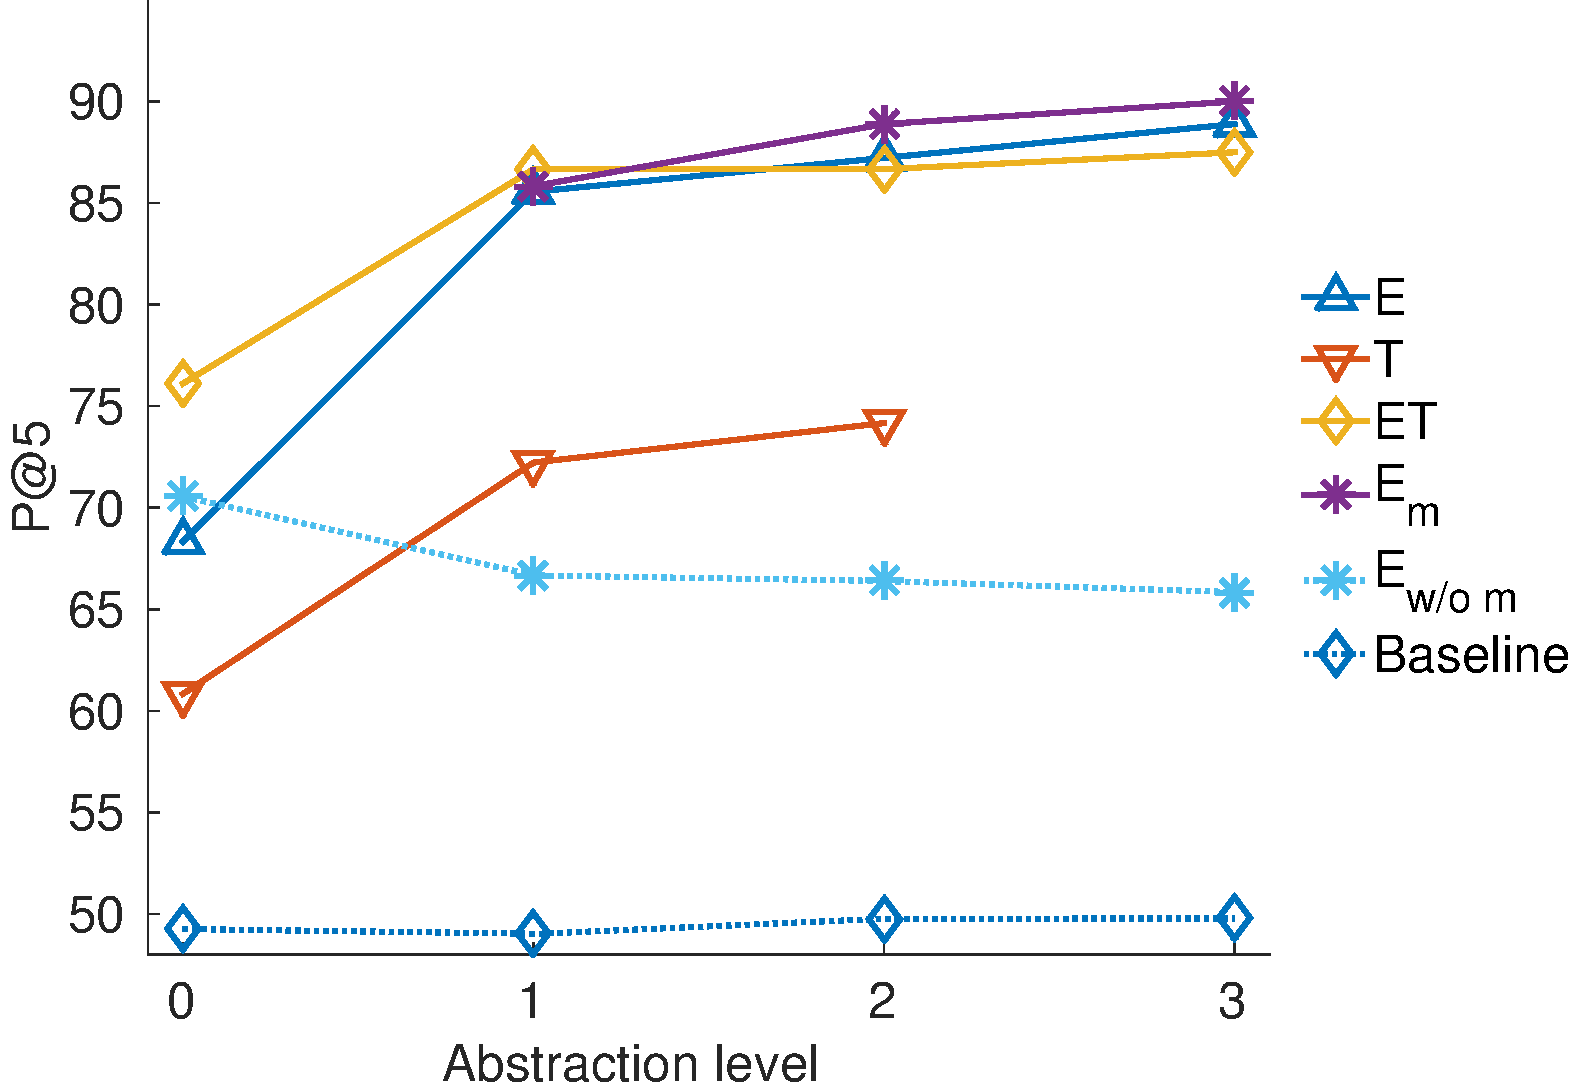
\includegraphics[width=\linewidth]{gfx/pa5_1_en}
       \caption{$P@5$ obtained by considering the dissimilarity matrix computed from the paired Hamming distances of the semantic features vectors as a function of the abstraction level. The vectors are built by using all the classes ($ET$), only the event classes ($E$), only the texture classes ($T$), only the event classes corresponding to sound markers ($E_m$), or only the event classes excluding sound markers $E_{w/o,m}$.}\label{fig:pa5}
\end{figure}

%Dans cette partie, nous évaluons la capacité d'une représentation sémantique à séparer les deux types d'environnement. Pour ce faire, nous calculons une précision au rang 5 ($p@5$) sur l'espace induit par les descripteurs sémantiques $S$, et ce pour chaque niveau d'abstraction (\cf~Section~\ref{sec:xp1_dataAna}). Les vecteurs $S$ sont construits en utilisant toutes les classes ($ET$), les classes d'événements ($E$), les classes de textures ($T$), les classes d'événements ne considérant que les marqueurs sonores ($E_m$), les classes d'événements ne considérant pas les marqueurs sonores $E_{w/o,m}$. Nous ne considérons pas les classes de marqueurs de textures, ces dernières étant trop peu nombreuses. Pour les mêmes raisons nous ne considérons pas les classes de marqueurs d'événements du niveau d'abstraction $0$. Les résultats sont affichés sur la figure~\ref{fig:pa5}.

In this section, we evaluate at which level a semantic representation of the scenes allows us to discriminate between the two types of environment. For this purpose, a rank 5-precision ($p@5$) is computed on the space induced by the semantic features $S$, and for each abstraction level, see Section~\ref{sec:xp1_dataAna}. The vectors $S$ are built by using all the classes ($ET$), only the event classes ($E$), only the texture classes ($T$), only the event classes corresponding to sound markers ($E_m$), or only the event classes excluding sound markers ($E_{w/o,m}$). Texture classes corresponding to sound markers are not numerous enough to reliably compute the metric. They are thus not considered. For the same reasons, event classes corresponding to sound markers at abstraction level $0$ are also discarded. Results are shown on Figure~\ref{fig:pa5}.

%En ce qui concerne $ET$, la $p@5$ est de $76\%$ pour le niveau d'abstraction 0, et reste supérieure à $86\%$ à partir du niveau d'abstraction 1. Ces résultats confirment qu'il est possible de clairement distinguer les deux types d'environnement en se basant seulement sur la présence ou l'absence des classes de sons. Nous notons également que, plus le niveau d'abstraction est élevé, plus la capacité de séparer les environnements est importante. En d'autres termes, plus nous sommes précis dans notre description de la composition des scènes, plus nous sommes à même d'établir une distinction claire entre les i- et ni-scènes.

Concerning $ET$, the $p@5$ is $76\%$ for the abstraction level $0$, and remains above $86\%$ for higher abstraction levels. Considering only the presence / absence of sound classes thus allows us to nicely discriminate between the two types of environments. We also notice that the higher the abstraction level is, thus the more precise the description, the more effective the description is.

%En considérant séparément $E$ et $T$, il apparaît 1) que la $p@5$ obtenue avec $E$ est similaire à celle obtenue avec $ET$, 2) que la $p@5$ obtenue avec $T$ est systématiquement inférieure d'environ $10$ à $15\%$ à celle de $E$. Ces résultats indiquent que l'information sémantique permettant de séparer les deux environnements est principalement portée par les événements. Ces résultats font, par ailleurs, écho aux travaux de  \cite{maffiolo_caracterisation_1999}, qui montrent que nous analysons de manière descriptive (en identifiant les sources) les scènes événementielles, \ie~composées d'événements sonores (\cf~Section~\ref{sec:simscene_sampleDataSet}).

Considering $E$ and $T$ separately, it appears that: 1) the $p@5$ obtained with $E$ is similar to the one obtained with $ET$ ; 2) the $p@5$ obtained with $T$ is always lower than the one obtained with $E$, by $10\%$ to $15\%$. Those results indicate that the semantic information that is discriminative is mostly carried by the events. Those results are in line with \cite{maffiolo_caracterisation_1999}. As discussed in Section~\ref{sec:simscene_sampleDataSet}, it seems that humans analyze the event scenes which are composed of several sound events in a causal manner, \ie by identifying the sources.

%Enfin, il apparaît que la $p@5$ obtenue avec $E_{m}$ est égale, voire supérieure à celles obtenues avec $E$ et $ET$, et ce bien qu'une information partielle soit utilisée dans ce cas pour décrire les scènes. La dimension des vecteurs de description $S$ pour $E_m$ est en effet inférieure à la dimension des vecteurs $S$ pour $E$, qui est elle même inférieure à celle obtenue dans le cas où toutes les classes sont utilisées ($ET$). De plus, dans le cas où les marqueurs ne sont pas pris en compte pour la description ($E_{w/o,m}$), les résultats chutent, passant même en dessous de ceux obtenus en ne considérant que les textures. Cela confirme que la majorité de l'information sémantique permettant de faire la distinction entre i-scènes et ni-scènes est incluse dans les marqueurs.

The dimension of the vectors $S$ for $E_m$ is lower than the dimension of vector $S$ for $E$, itself lower than the dimension of vector $S$ obtained when all the classes are considered ($ET$). $S$ being a boolean vector, the smaller the dimension, the lower the amount of information it can carry. Despite this, it appears that the $p@5$ obtained with $E_m$ is equal – or above – to the ones obtained with $E$ or $ET$, although only a partial information is used in that case to describe the scenes. On the opposite, if the sound markers are not taken into account for the description ($E_{w/o,m}$), the performance is below the one achieved when considering only the textures as features. Thus, most of the semantic information allowing to differentiate between i- and ni-scenes is included in the markers.

%En résumé, nous déduisons de cette analyse les points suivants:
%
%\begin{enumerate}
%\item contrairement à ce que nous avions constaté avec les descripteurs structurels, une description sémantique de la composition des scènes, en terme de présence/absence de sources sonores, permet de bien distinguer les deux types d'environnement (i ou ni);
%\item l'information sémantique est majoritairement portée par les classes d'événements sonores;
%\item parmi les classes d'événements, seule une partie, \ie~les marqueurs sonores, est nécessaire pour faire la distinction entre les i- et ni-scènes.
%\end{enumerate}

The outcomes of this analysis are:

\begin{enumerate}
\item unlike what we outlined with the sound levels, a semantic description of the scenes composition in terms of presence / absence of sound sources, allows us to differentiate reliably the two types of environments (i or ni);
\item the semantic information is mainly contained in the event sound classes;
\item only a part of the event classes, i.e. the sound markers, are useful to differentiate between the i- and ni-scenes.
\end{enumerate}

%Maintenant que nous avons isolé les classes typiques des i- et ni-scènes, et vérifié que la distinction entre ces environnements dépendait de la présence de ces classes, il reste à voir si une description structurelle des scènes, basée uniquement sur ces marqueurs sonores, permet de caractériser l'agrément perçu, mieux qu'une description structurelle globale.

Since we have extracted the typical classes of the i- and ni-scenes and verified that the distinction between them was largely dependent on the presence of these classes, we shall now investigate whether a description of the scenes only based on the sound pressure level of sound markers could characterize the perceived pleasantness, perhaps better than a globally computed sound level.

\subsubsection*{Influence of the sound markers on the perceived pleasantness}

\begin{table}[t]
\setlength{\tabcolsep}{3pt}
\centering
{\renewcommand{\arraystretch}{1}
\centering
\begin{tabular}{l r r}
                  &   i-scenes                  & ni-scenes \\
\hline
$L_m$              & 0.03  ($p=0.88$)           & \textbf{-0.75} ($p<0.01$) \\
$L(E)_m$           & 0.08  ($p=0.66$)           & \textbf{-0.71} ($p<0.01$) \\
$L(T)_m$           & -0.11 ($p=0.66$)           & -0.17 ($p=0.37$) \\
$L_b$              & \textbf{-0.52} ($p<0.01$)  & -0.32 ($p=0.06$) \\
$L(E)_b$           & \textbf{-0.51} ($p<0.01$)  & -0.30 ($p=0.07$) \\
$L(T)_b$           & -0.32 ($p=0.05$)           & \textbf{-0.73} ($p<0.01$) \\
$L_m-L_b$          & \textbf{0.67} ($p<0.01$)   & -0.31 ($p=0.07$) \\
$L(E)_m-L(E)_b$    & \textbf{0.66} ($p<0.01$)   & -0.28 ($p=0.10$) \\
$L(T)_m-L(T)_b$    & 0.16 ($p=0.54$)            & 0.21 ($p=0.28$) \\
\hline
\end{tabular}
}
\vspace{0.5mm}
\caption{Linear correlation coefficients computed between mean perceived pleasantness $\mathcal{A}_{scene}$ (Exp. 1.b) and sound levels related to the presence of sound markers.}
\label{tab:corrMarkers}
\end{table}

\begin{figure}[t]
        \myfloatalign
        \subfloat[]
        {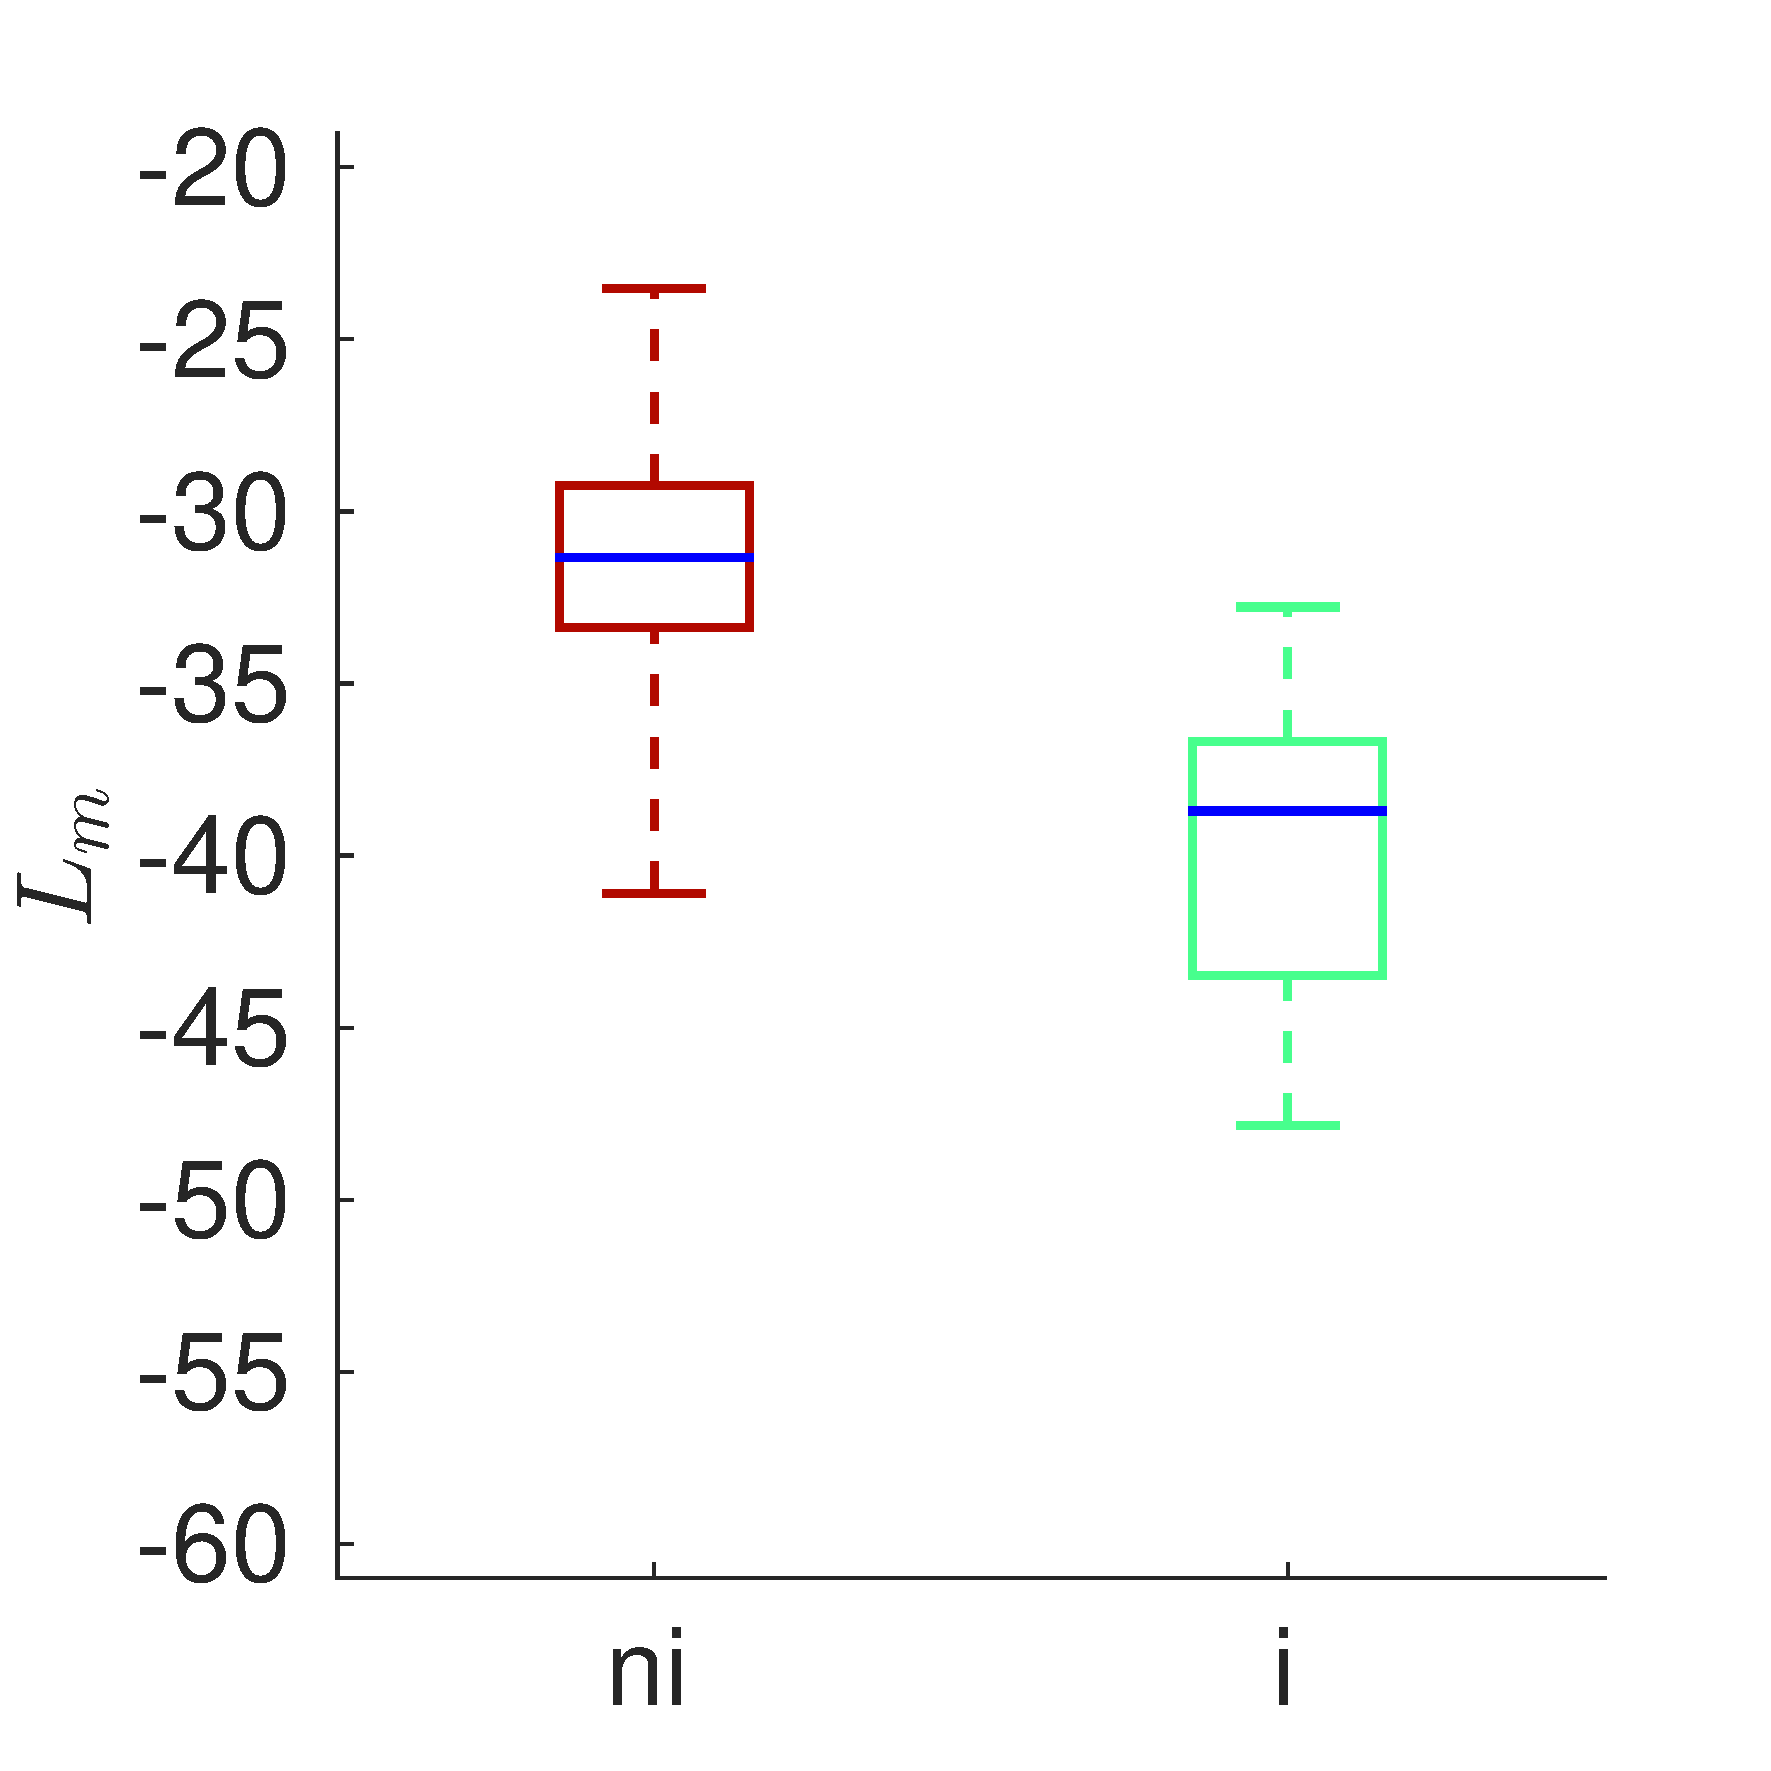
\includegraphics[width=.33\linewidth]{gfx/xp_soundlevel_7}\label{fig:soundlevelMarkera}}
        \subfloat[]
        {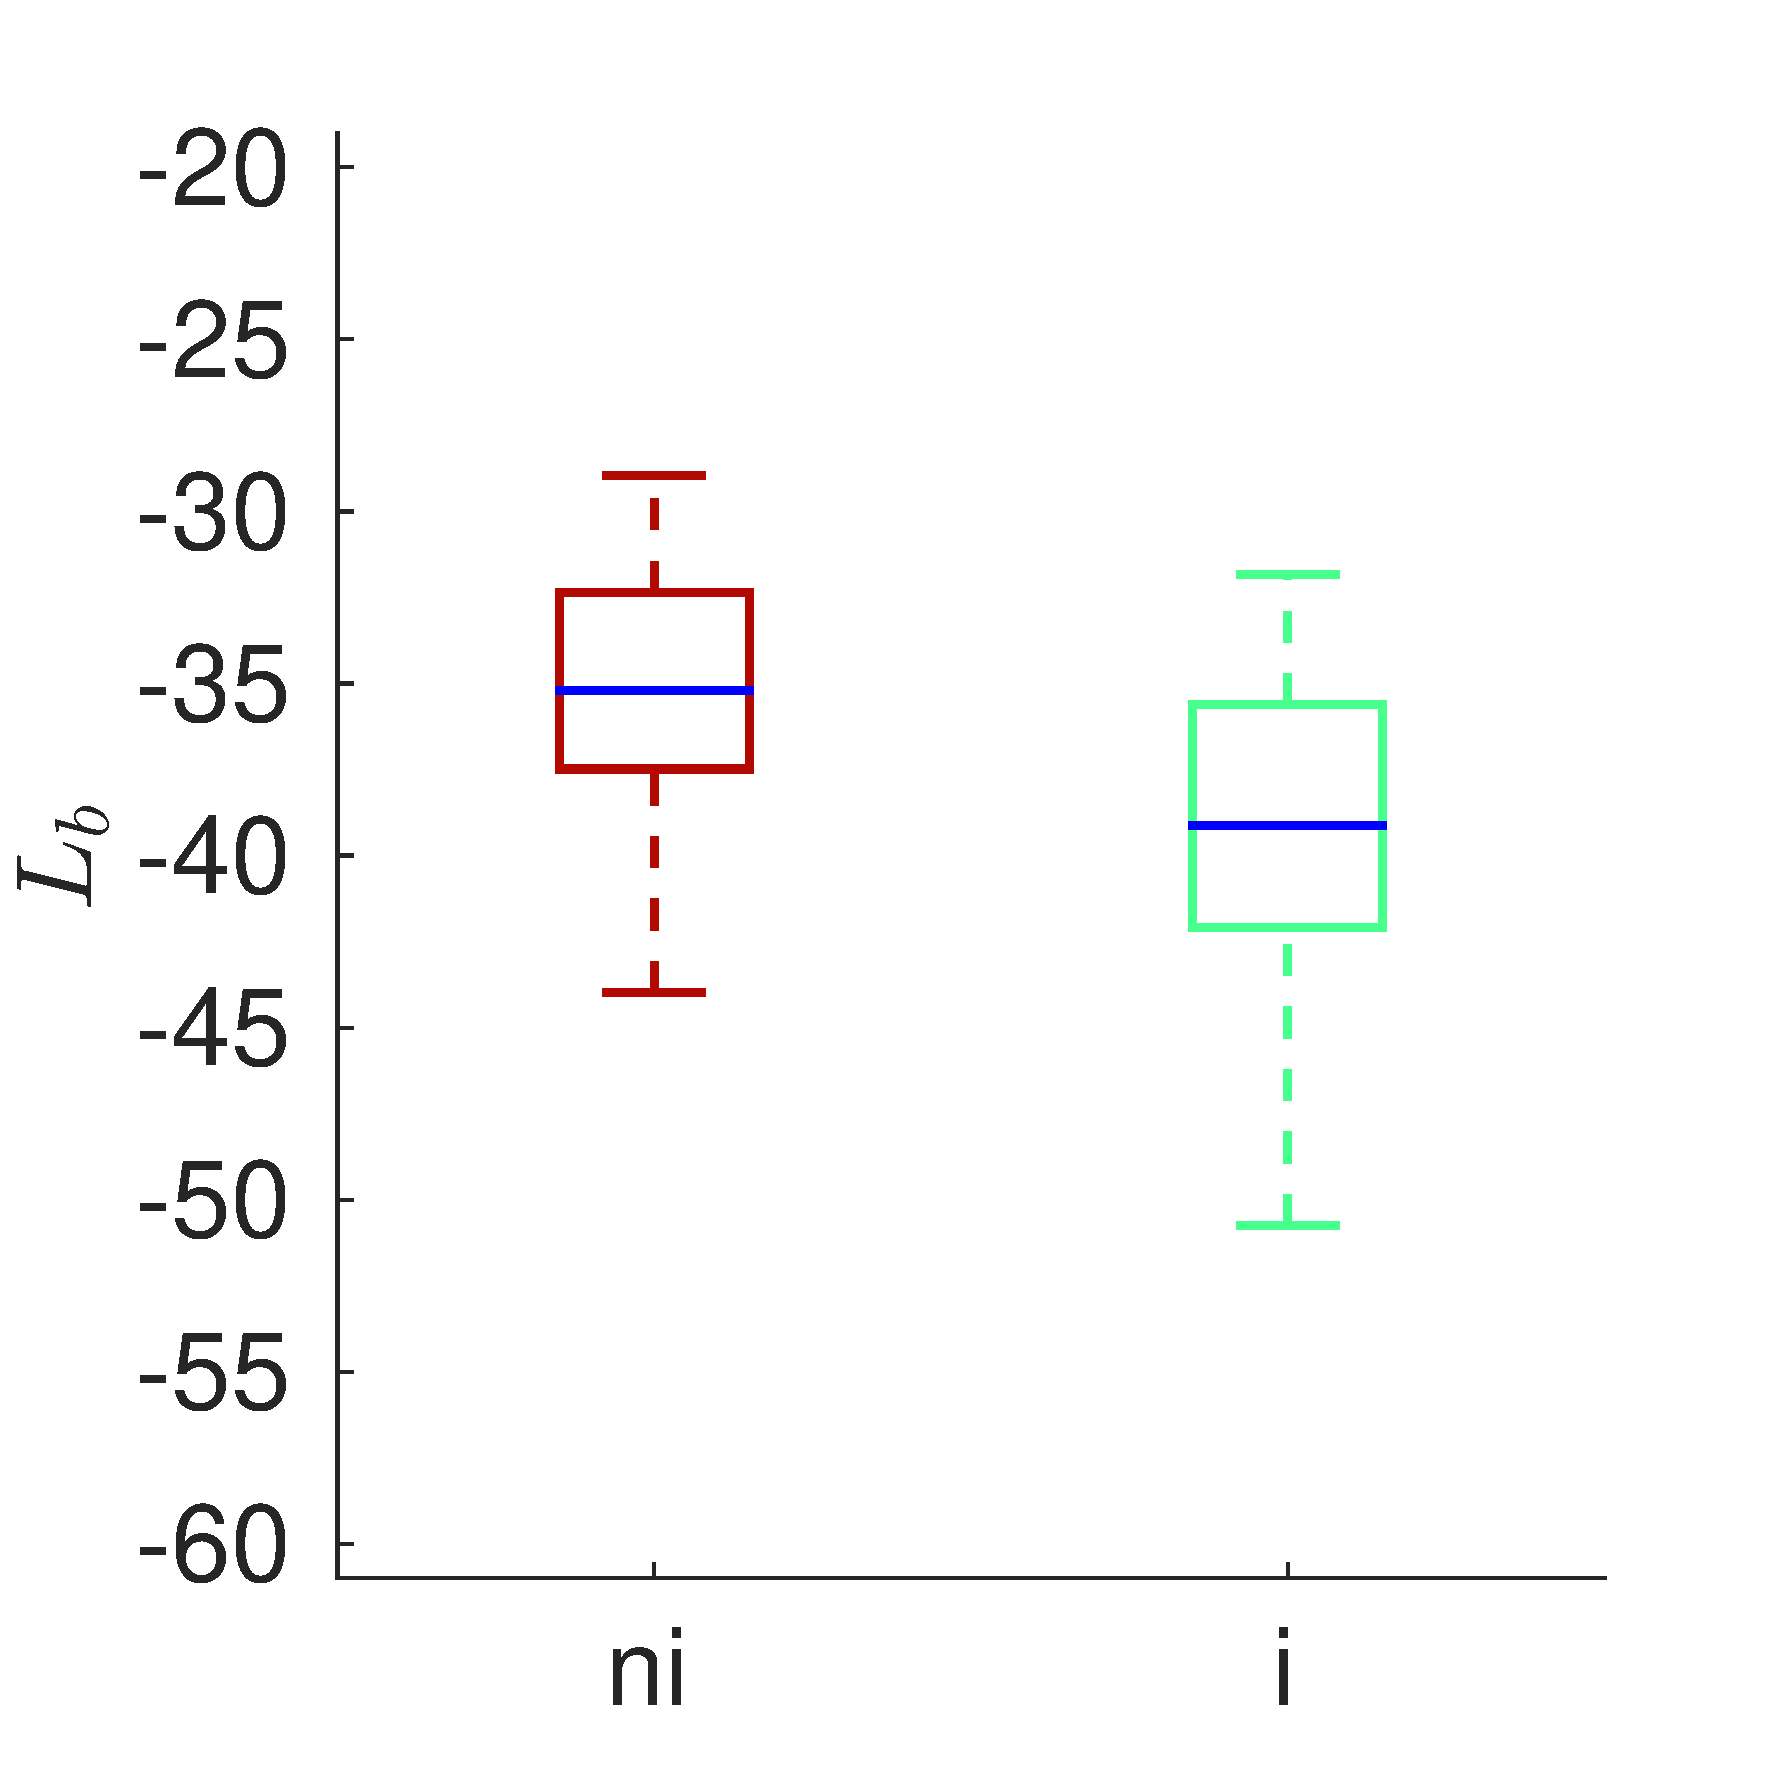
\includegraphics[width=.33\linewidth]{gfx/xp_soundlevel_9}\label{fig:soundlevelNoisea}}
        \subfloat[]
        {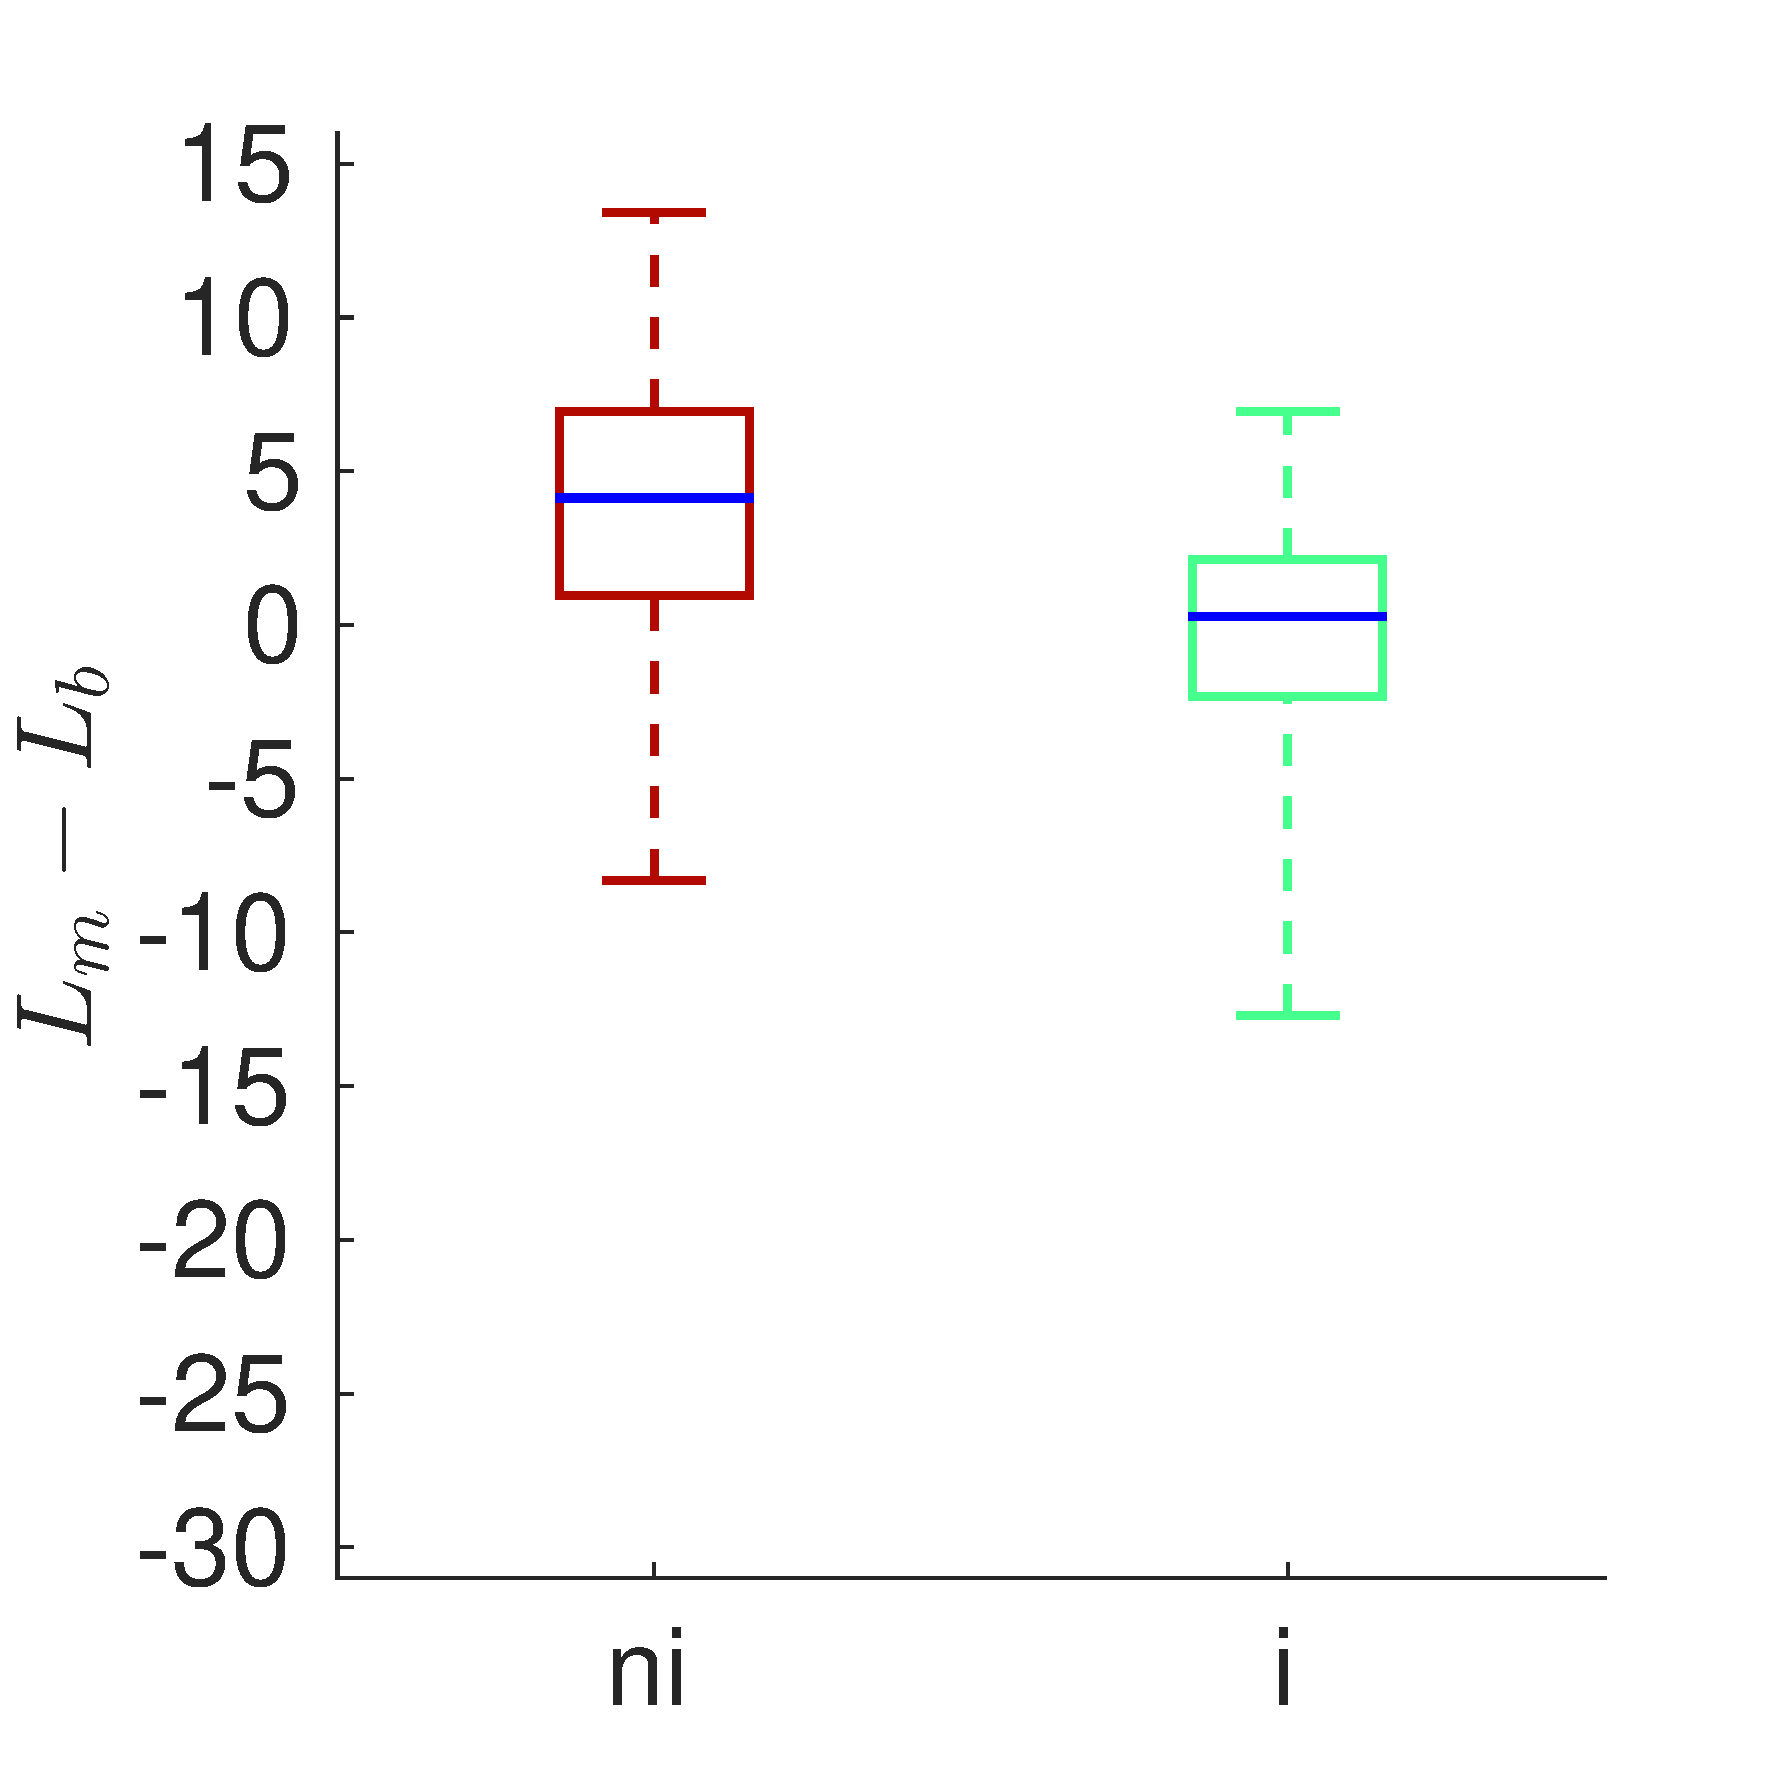
\includegraphics[width=.33\linewidth]{gfx/xp_soundlevel_19}\label{fig:soundlevelMarkerDiffa}}\par
        \subfloat[]
        {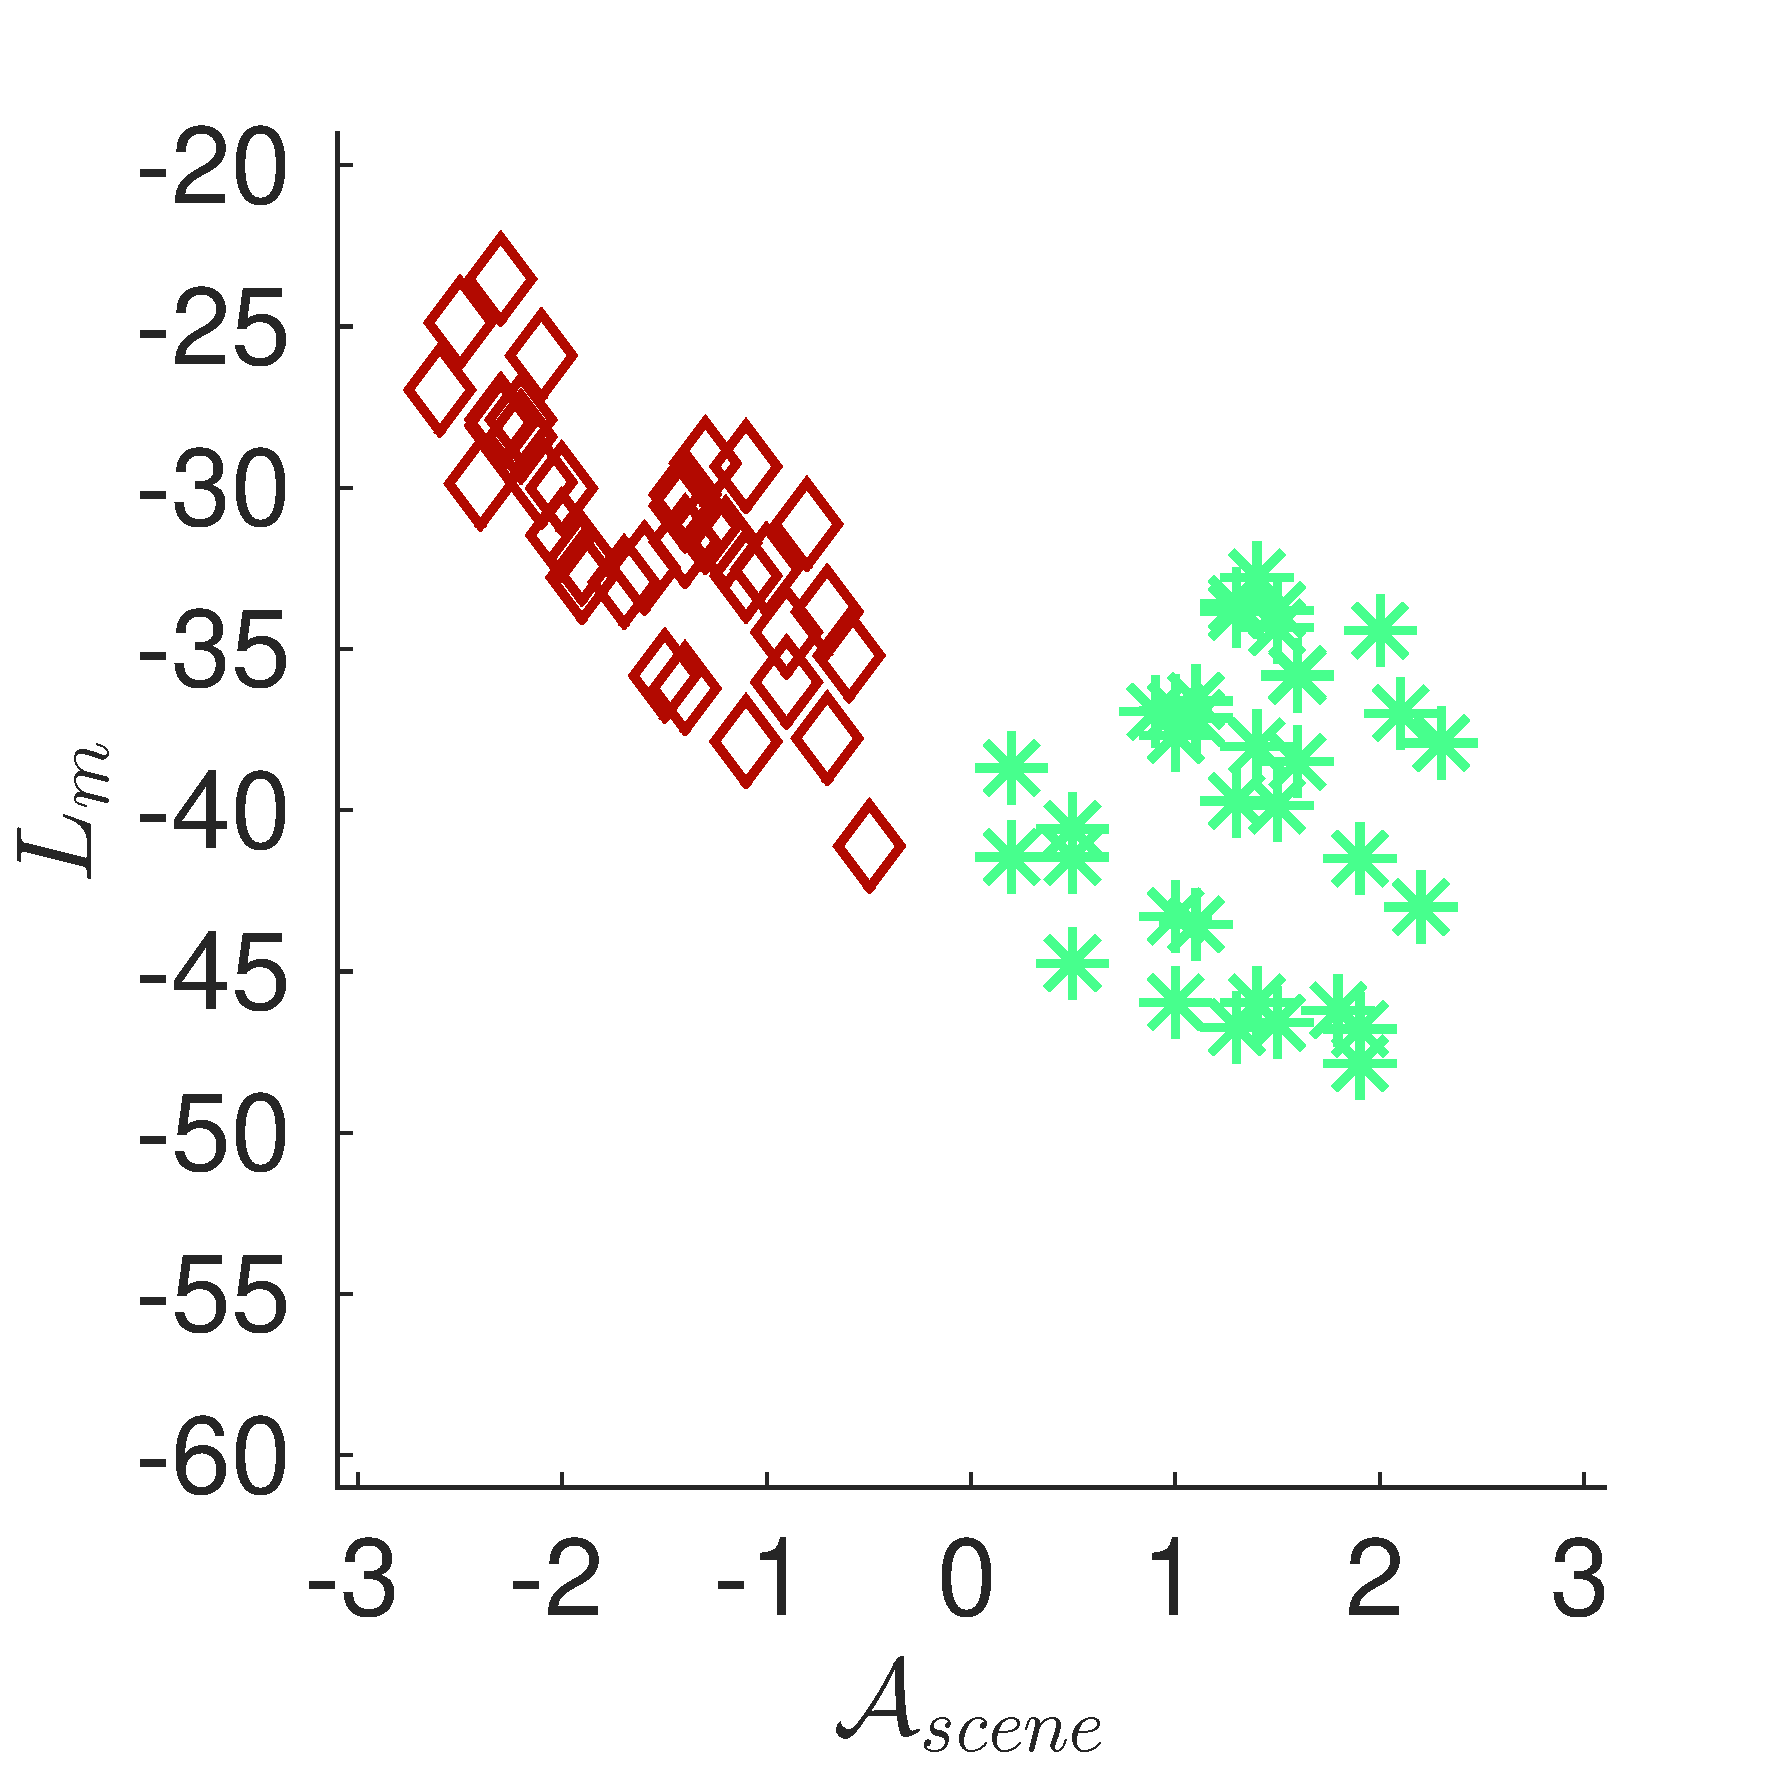
\includegraphics[width=.33\linewidth]{gfx/xp_soundlevel_8}\label{fig:soundlevelMarkerd}}
        \subfloat[]
        {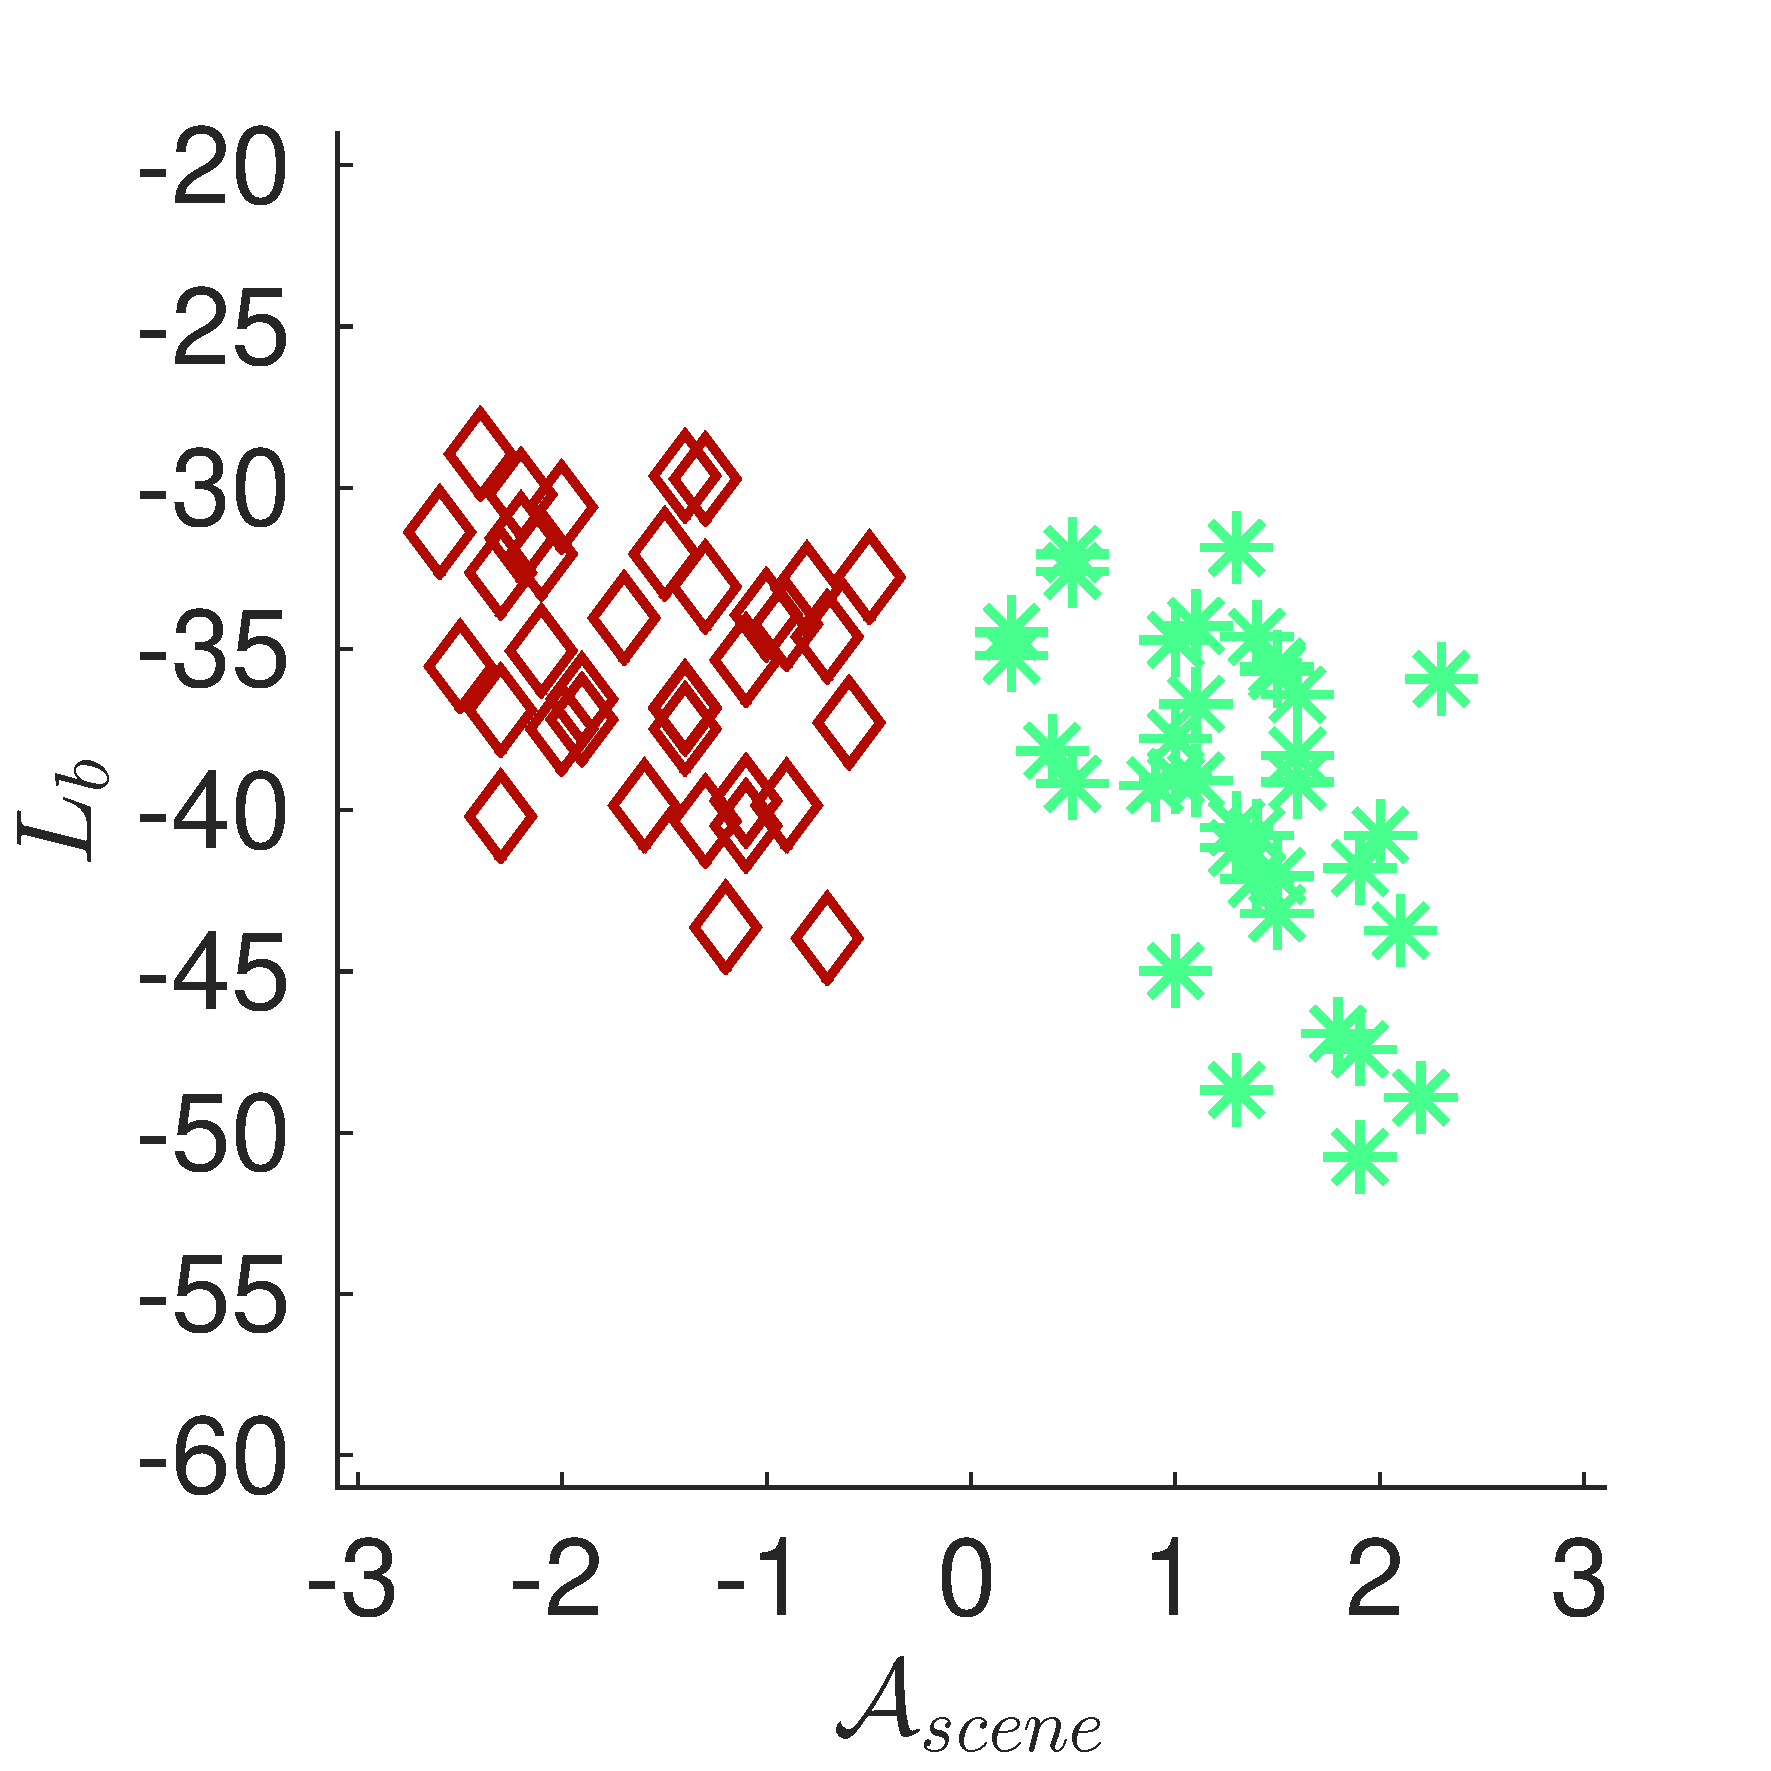
\includegraphics[width=.33\linewidth]{gfx/xp_soundlevel_10}\label{fig:soundlevelNoised}}
        \subfloat[]
        {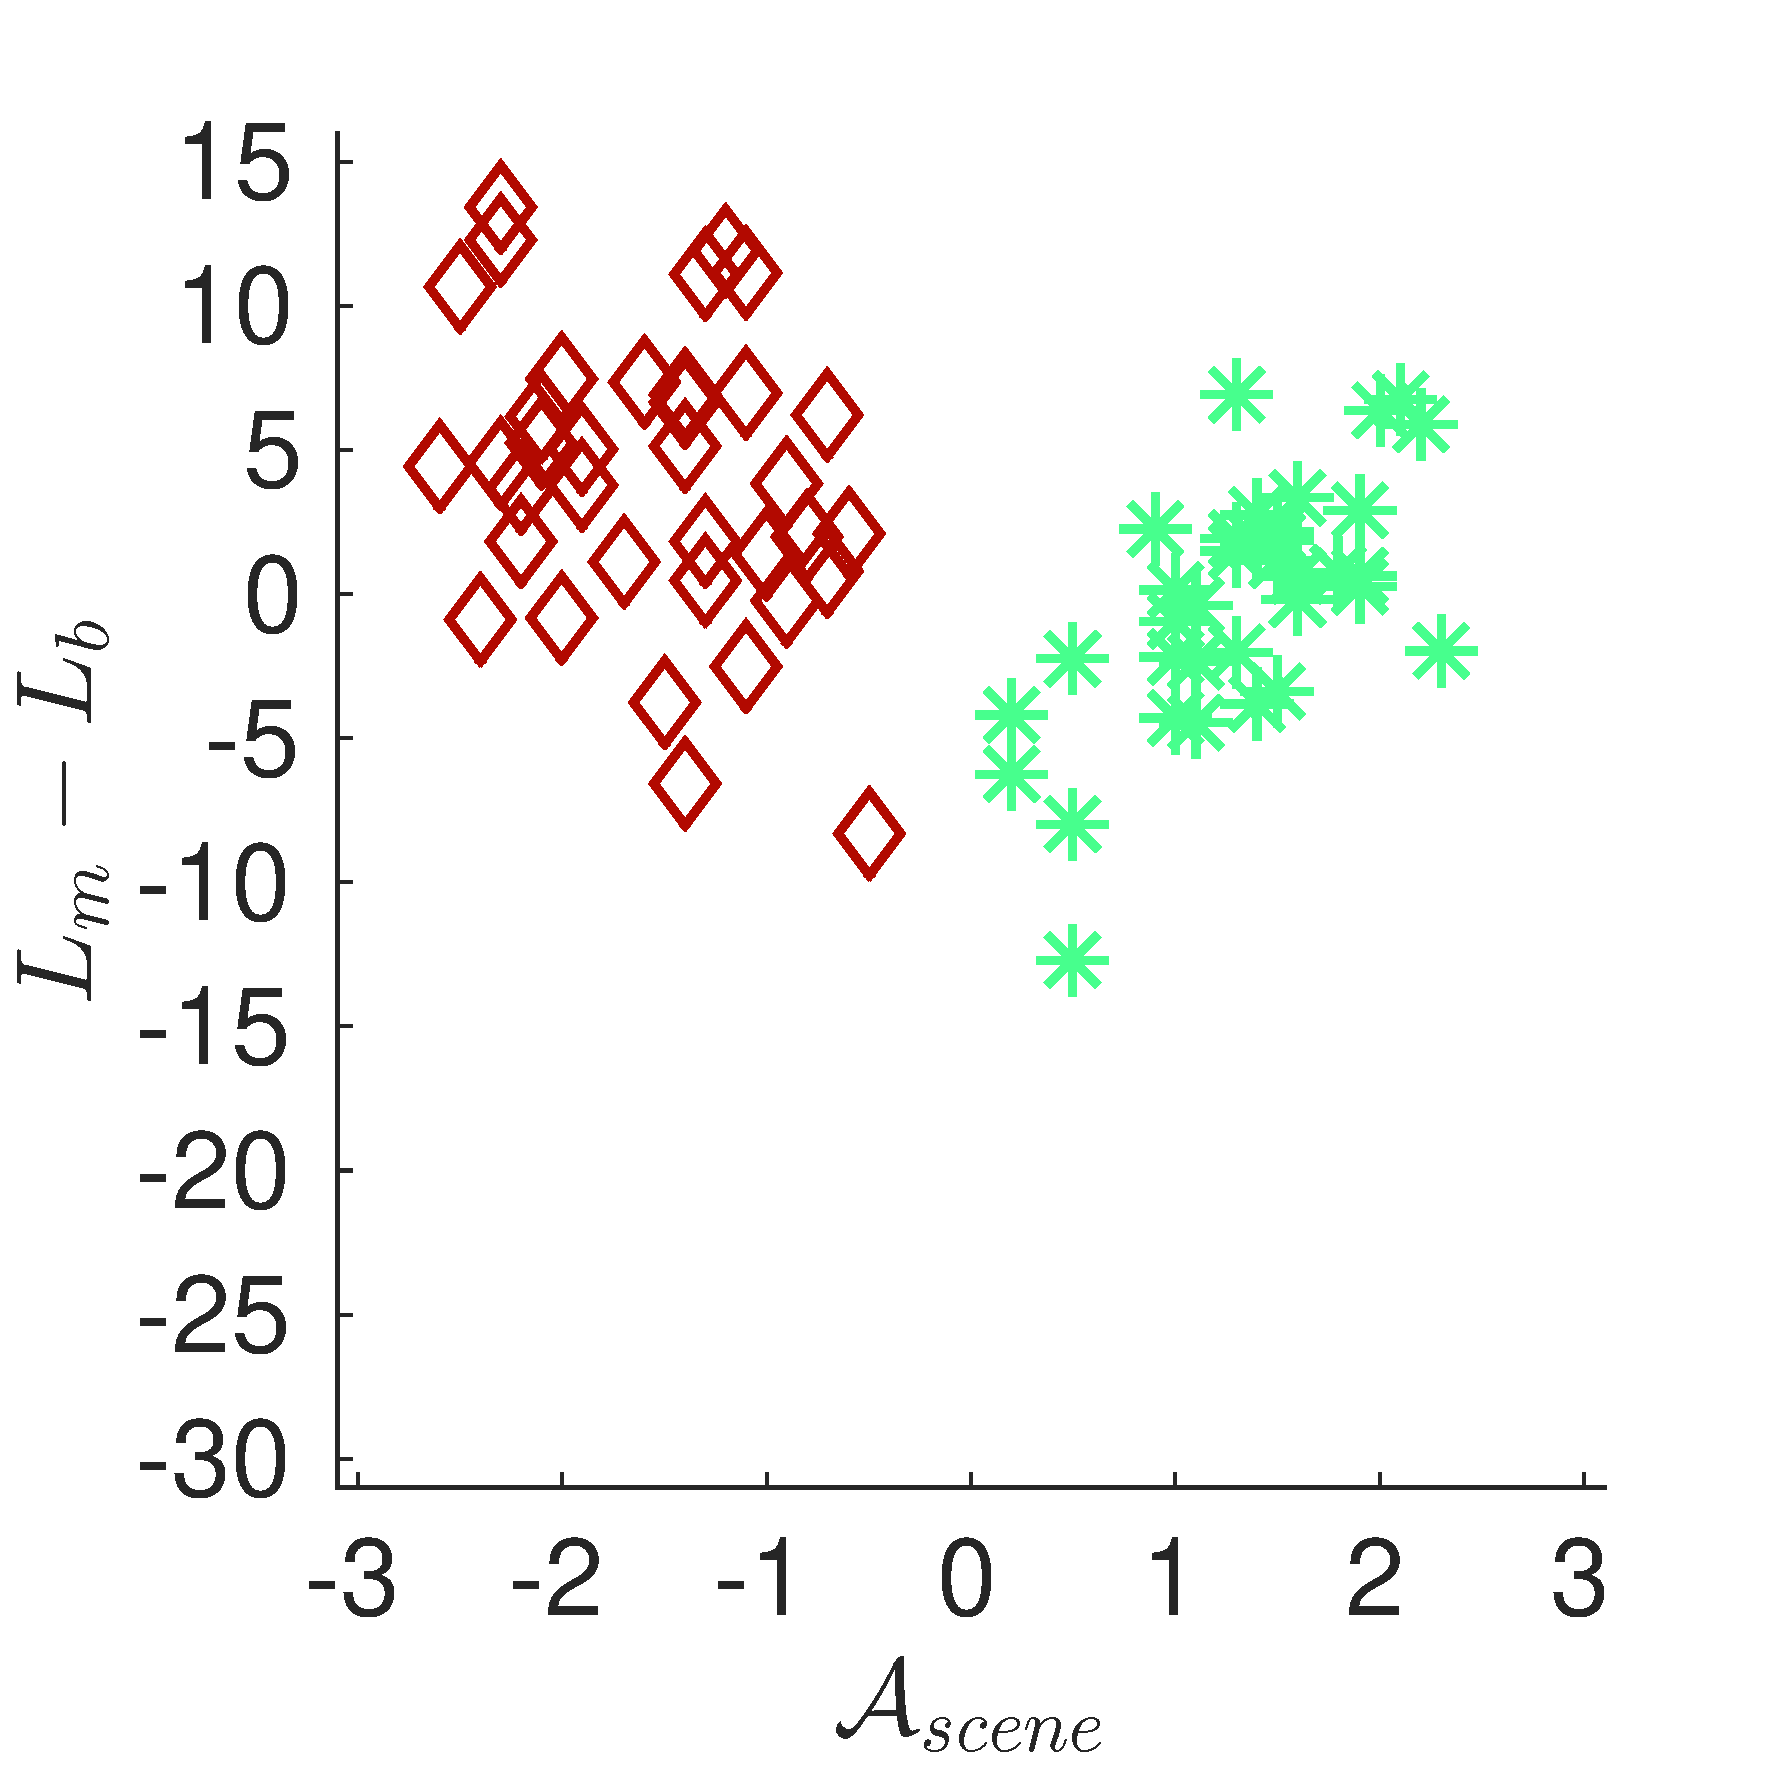
\includegraphics[width=.33\linewidth]{gfx/xp_soundlevel_20}\label{fig:soundlevelMarkerDiffd}}
        \caption{Distribution of the relative sound levels related to the presence of markers $L_m$ (a, d), $L_b$ (b, e) and $L_m-L_b$ (c, f), versus scene type (a, b, c) and perceived pleasantness $\mathcal{A}_{scene}$ of experiment 1.b (d, e, f).}\label{fig:soundlevelMarker}
\end{figure}

%Nous évaluons les corrélations entre $\mathcal{A}_{scene}$ et les descripteurs structurels. Pour cette section, les descripteurs structurels sont calculés en tenant compte des marqueurs sonores précédemment identifiés. Nous définissons $X_m$ le descripteur $X$ calculé en ne prenant en compte que les sons des marqueurs. A l'inverse, nous définissons $X_b$ ($b$: pour «~bruit~») le descripteur $X$ calculé en prenant en compte toutes les classes de sons, excepté les marqueurs. Lorsque le descripteur caractérise une i-scène (idem pour une ni-scène), nous ne considérons, pour le calcul, que les marqueurs identifiés pour les i-scènes (ou pour les ni-scènes), que nous nommons i-marqueurs (ou ni-marqueurs). Les résultats sont affichés sur le tableau~\ref{tab:corrMarkers}.

To do so, the correlations between $\mathcal{A}_{scene}$ and the sound levels are evaluated. In this section, the sound levels are computed by taking into account only the previously identified sound markers. We define $X_m$, the $X$ feature computed by taking into account only the sound markers. On the opposite, we define $X_b$, the $X$ feature computed by taking into account all the sound classes, except the sound markers. When the feature characterizes an i-scene (idem for a ni-scene),  only the markers identified for the i-scenes (or the ni-scenes) are considered; we named them, i-markers (or ni- markers). Results are shown in Table~\ref{tab:corrMarkers}.

%Concernant les niveaux sonores (\cf~Figures~\ref{fig:soundlevelMarkera} et~\ref{fig:soundlevelMarkerd}), les mêmes tendances sont observées entre $L_m$, $L(E)_m$ et $L(T)_m$, d'une part, et $L$, $L(E)$ et $L(T)$, d'autre part. Que l'on considère uniquement les marqueurs, ou l'ensemble des classes, il s'avère que :

Concerning the sound levels, the same trends are measured between $L_m$, $L(E)_m$ and $L(T)_m$ on one side, and $L$, $L(E)$ and $L(T)$ on the other side, see~Figures~\ref{fig:soundlevelMarkera} and~\ref{fig:soundlevelMarkerd}, respectively. No matter whether all the classes or only the markers are considered, it appears that:

%\begin{enumerate}
%\item il existe une différence significative entre les niveaux des i- et ni-scènes ($L_m$, $L(E)_m$ et $L(T)_m$: $p<0.01$);
%\item le niveau sonore des scènes est majoritairement porté par les événements sonores, comparé aux textures sonores;
%\item le niveau sonore des événements a une influence sur la perception de l'agrément pour les ni-scènes, mais pas pour les i-scènes;
%\item le niveau sonore des textures ne joue aucun rôle dans la perception de l'agrément.
%\end{enumerate}

\begin{enumerate}
\item a significant difference between levels of i- and ni-scenes exists ($L_m$, $L(E)_m$ et $L(T)_m$: $p<0.01$);
\item the sound level of scenes is mainly related to the sound events, compared to the textures;
\item the sound level of events has an influence on the perception of pleasantness for ni-scenes, but not for i-scenes;
\item the sound level of textures does not play any role in the perception of the pleasantness.
\end{enumerate}

%En conclusion, le niveau des ni-marqueurs a une influence négative sur l'agrément pour les ni-scènes. En revanche le niveau des i-marqueurs n’impacte pas l'agrément perçu pour les i-scènes.

To conclude, the level of ni- markers has a negative influence on the pleasantness for the ni-scenes. On the other hand, the level of i- markers does not influence the perceived pleasantness for the i-scenes.

% En considérant maintenant les classes non marqueurs (\cf~Figures~\ref{fig:soundlevelNoisea} et~\ref{fig:soundlevelNoised}), nous remarquons, sur les i-scènes, une corrélation négative modérée/faible pour $L_b$  ($r=-52$, $p<0.01$) et $L(E)_b$ ($r=-51$, $p<0.01$). C'est la première fois qu'un indicateur objectif nous permet de préciser l'agrément des environnements agréables. Ceci nous amène à conclure que le niveau des classes de sons n'étant pas typiques d'un environnement agréable a un impact négatif sur l'agrément.

Considering the non markers classes, we can observe on the i-scenes results, a weak negative correlation for $L_b$  ($r=-52$, $p<0.01$) et $L(E)_b$ ($r=-51$, $p<0.01$), see Figures~\ref{fig:soundlevelNoisea}  and ~\ref{fig:soundlevelNoised}. It is the first time that an objective feature allows us to define the pleasantness of i-scenes. This leads us to conclude that the level of non-typical sound classes of a pleasant environment has a negative influence on the pleasantness.

% Par ailleurs, alors que $L(T)$ ne présentait pas de corrélation pour les ni-scènes, une corrélation négative forte est observée pour $L(T)_b$ ($r-0.73$, $p<0.01$). Ce fait indique que les niveaux des classes de textures n'étant pas des marqueurs n'affectent pas l'agrément perçu de la même manière pour les i- et ni-scènes. Les niveaux semblent avoir un effet négatif pour les ni-scènes, alors que pour les i-scènes, aucun effet n'est relevé.

Alos, whereas $L(T)$ did not show any significant correlation for ni-scenes, a strong negative correlation is observed for $L(T)_b$ ($r = -0.73$, $p < 0.01$). This indicates that the level of non-markers texture classes does not influence the perceived pleasantness in the same way for i- and ni-scenes. Sound level seems to have a negative effect for the ni-scenes, and no significant effect for the i-scenes.

% Pour finir, nous considérons un dernier groupe de descripteurs, nommément $L_m-L_b$, $L(E)_m-L(E)_b$ et $L(T)_m-L(T)_b$ (\cf~Figures~\ref{fig:soundlevelMarkerDiffa} et~\ref{fig:soundlevelMarkerDiffd}). Ces descripteurs expriment la différence entre les niveaux des marqueurs, et ceux des autres classes de sons. Ils traduisent l'émergence des marqueurs par rapport à la mixture sonore.

A last group of features is now considered, namely $L_m-L_b$, $L(E)_m-L(E)_b$ and $L(T)_m-L(T)_b$.  These features describe the difference between the markers level and those of the other sound classes, see ~Figures~\ref{fig:soundlevelMarkerDiffa} and~\ref{fig:soundlevelMarkerDiffd}. They express the saliency of the markers with respect to the sound mixture.

% Pour les i-scènes, une corrélation modérée et positive est observée pour $L_m-L_b$ ($r=0.67$, $p<0.01$) et $L(E)_m-L(E)_b$ ($r=0.66$, $p<0.01$). Pour les ni-scènes, aucune corrélation n'est observée. Dans le cas des i-scènes, ce n'est donc pas le niveau absolu des marqueurs qui importe, mais leur niveau relatif, par rapport aux autres sons qui composent la scène. On observe donc pour les environnements idéaux un double mécanisme perceptif:

For the i-scenes, a moderate positive correlation is observed for $L_m-L_b$ ($r=0.67$, $p<0.01$) and $L(E)_m-L(E)_b$ ($r=0.66$, $p<0.01$). for the ni-scenes no correlation is observed. Thus, for the i-scenes, it is not the absolute markers level that is important, but their relative level with respect to the other sounds composing the scene. A double perceptual mechanism for the ideal environments: can thus be observed:

%\begin{itemize}
%\item plus le niveau absolu des sons n'étant pas des i-marqueurs est élevé, plus l'agrément est faible,
%\item plus le niveau relatif des i-marqueurs, par rapport aux autres sons, est élevé, plus l'agrément est élevé.
%\end{itemize}

\begin{itemize}
\item the higher the absolute level of sounds not being i-markers, the weaker the pleasantness,
\item the higher the relative level of i-markers is, with respect to the remaining sounds, the higher the pleasantness.
\end{itemize}

%Pour les ni-scènes, le fait que nous observions des corrélations pour $L_m$ et $L(E)_m$, et aucune pour $L_m-L_b$ et $L(E)_m-L(E)_b$, montre que c'est bien le niveau absolu qui importe.

On contrary, the fact that we observe significant correlations for $L_m$ and $L(E)_m$ and no correlation for $L_m-L_b$ and $L(E)_m$ - $L(E)_b$ for the ni-scenes, shows that this is indeed the absolute level that matters.

\subsection{Discussion}

%De cette analyse, nous retenons les points suivants:

From this analysis, the following points can be outlined:

\begin{itemize}

%\item \emph{distinguer les i- et ni-scènes}: les descripteurs sémantiques, ainsi que les descripteurs structurels globaux ($L$, $L(E)$ et $L(T)$), permettent de faire la distinction entre les i-scènes et les ni-scènes. La description sémantique semble être plus performante;
%\item \emph{événements ou textures}: que ce soit pour les descripteurs sémantiques ou structurels, ce sont majoritairement les événements qui permettent de distinguer les deux types d'environnement, les textures n'apportant, au mieux, qu'une information limitée;
%\item \emph{prédire l'agrément}: si l'on considère les corrélations entre les descripteurs structurels et l'agrément, il semble que la manière de percevoir la qualité de l'environnement diffère en fonction de la nature de ce dernier (i ou ni). Il n'apparaît pas envisageable de considérer un même jeu de descripteurs pour prédire, à la fois, l'agrément des i-scènes, et l'agrément des ni-scènes :

\item \emph{differentiating the i- and ni-scenes}: the semantic features, and the global sound levels ($L$, $L(E)$ et $L(T)$), allow us to differentiate reliably between i- and ni-scenes. The semantic description seems to be more powerful;
\item \emph{events or textures}: whatever the feature type, be it semantic or related to the sound pressure level, events are the most useful components of the scene to differentiate the two types of scenes; textures bring a limited amount of information;
\item \emph{pleasantness prediction}: considering the correlation between sound levels and pleasantness, it seems that the way subjects perceived the quality of a given environment depends on its very nature (i or ni). From the data gathered in those experiments, the same set of features cannot be considered to predict the pleasantness of i- and ni-scenes:

\begin{itemize}

%\item \emph{pour les ni-scènes}, ce sont le niveau global ($L$ et $L(E)$), ou le niveau des marqueurs sonores ($L_m$ et $L(E)_{m}$), qui impactent négativement l'agrément. On note ici que prendre en compte les contributions de différentes sources n'améliore pas la capacité de prédiction de l'agrément, par rapport à une analyse holistique de l'environnement.

\item \emph{for ni-scenes}, the global levels ($L$ et $L(E)$), or the level of sound markers ($L_m$ et $L(E)_{m}$), have a negative influence on pleasantness. Taking into account the contribution of each of the different sources of the scene does not improve the prediction performance compared to a global analysis of the environment.

%\item \emph{pour les i-scènes}, par contre, prédire l'agrément requiert d'étudier, de manière séparée, les caractéristiques des marqueurs sonores, et celles de l'ensemble des autres sons. Ainsi, le niveau des marqueurs pris relativement au bruit ($L(E)_m-L(E)_b$ et $L_m-L_b$) est positivement corrélé à l'agrément, alors que le niveau du bruit ($L_b$ et $L(E)_b$) est, lui, négativement corrélé.

\item \emph{for i-scenes}, on contrary, the sound markers characteristics and those of the other sounds have to be considered separately to predict  the pleasantness. The markers level, relative to the background noise ($L(E)_m-L(E)_b$ and $L_m-L_b$) is positively correlated to the pleasantness, whereas the noise level ($L_b$ and $L(E)_b$) is negatively correlated.

\end{itemize}
\end{itemize}

%Le fait que l'agrément des i-scènes ne se corrèle pas avec des descripteurs physiques holistiques, contrairement à l'agrément des ni-scènes, a récemment été déjà observé \cite{gozalo2015relationship}.

The fact that the pleasantness of the i-scenes is not correlated to global physical features, contrary to pleasantness of ni-scenes, has also been studied recently \cite{gozalo2015relationship}.

%L'existence de deux modes de perception, mobilisant différents types de descripteurs, et dépendant de la nature (dans notre cas hédonique) des stimuli, est un phénomène qui se rapproche de celui observé pour la perception des textures (\cf~Section~\ref{sec:simscene_sampleDataSet}). Le cerveau adapte sa manière de traiter l'information (résumé statistique pour les textures, description fine pour les événements) suite à une prise de décision antérieure quant à la nature du stimulus (à savoir «~est-ce un événement ou une texture ?~»). De la même manière, les indicateurs actifs dans le jugement de l'agrément dépendent, eux aussi, d'une identification préalable de la nature hédonique globale de l'environnement (idéale ou non idéale).

We can assume two perceptual modes of operation that involve different types of features and rely on the hedonic nature  of the stimuli. It thus appears that the features considered for the pleasantness judgment also depends on a preliminary judgment of the global hedonic nature of the environment (ideal or non ideal).

A similar phenomenon is observed for the perception of textures, see Section~\ref{sec:simscene_sampleDataSet}. It seems that the brain selectively adapts the way it encodes the information (statistic summary for textures, finer description for events) following a previous decision making process based on the nature of the stimuli, \ie~is it an event or a texture ?

\section{Experiment 2: modification of the semantic content}
\label{sec:modification}

\subsection{Objective}

%L'expérience précédente a montré que, parmi les classes de sons peuplant le monde sonore, celles regroupant les marqueurs sont caractéristiques de certains types d'environnement. Ces marqueurs sonores semblent avoir un impact particulier sur la perception de leurs environnements. C'est ce dernier point qui est étudié dans cette expérience.

The previous experiment demonstrated that, among the classes of sounds occurring in urban soundscapes, those with markers are specific to some environments. Those sound markers seem to have a great impact on perception. This impact is studied here in more detail using an added benefit of the simulation paradigm proposed in this paper, the ability to manipulate and modify the generated scenes.

%Afin de vérifier que l'agrément des scènes idéales et non-idéales dépend de la présence des marqueurs, les scènes sonores précédemment simulées sont régénérées, sans les classes de marqueurs. Pour les i-scènes, les i-marqueurs sont retirés. Pour les ni-scènes, les ni-marqueurs. Une épreuve d'évaluation de l'agrément, dont le protocole se rapproche de celui de l'expérience 1.b, est alors conduite.

In order to investigat deeper into the relation between the pleasantness of the ideal and non ideal scenes and the sound markers, the audio waveform of the simulated scenes are regenerated with or without the classes identified as markers. To do so, some of the i-markers are removed for the i-scenes and some of the ni-markers are removed for the ni-scenes. To evaluate the impact on the perception of pleasantness caused by those modifications, a perceptual test is conducted with a protocol close to the one considered in experiment 1.b.

%L'objectif est de vérifier si l'absence des marqueurs a un impact sur l'agrément perçu. Deux hypothèses sont formulées:

The objective of this experiment is to study if the removal of the previously identified markers have an impact on the perceived pleasantness. Two hypothesis are thus formulated:

%\begin{itemize}
% \item \emph{pour les ni-scènes} nous faisons l'hypothèse que l'absence des ni-marqueurs va \textbf{augmenter} la valeur de l'agrément perçu;
% \item \emph{pour les i-scènes} nous faisons l'hypothèse que l'absence des i-marqueurs va \textbf{diminuer} la valeur de l'agrément perçu.
% \end{itemize}

\begin{itemize}
\item \emph{for the ni-scenes}, we hypothesize that the absence of ni-markers will \textbf{increase} the pleasantness score;
\item \emph{for the i-scenes}, we hypothesize that the absence of the i-markers will \textbf{decrease} the pleasantness score.
\end{itemize}

%Si la première hypothèse est intuitive, la deuxième l'est moins. En effet, il n’apparaît pas évident que la suppression des i-marqueurs, bien que s'agissant de sons positivement connotés, diminue la qualité globale d'un environnement. Cette suppression aura, de surcroît, pour effet de diminuer le niveau sonore global de la scène.

If the first hypothesis is rather intuitive, the second is less. Indeed, it is not obvious that the removal of the i-markers, though perceptively positively connoted, decreases the global quality of a soundscape. Indeed, this removal also decreases the global sound level of the scene.

%Néanmoins, comme nous l'avons vu, le niveau global n'est qu'un indicateur partiel de l'agrément pour les environnements sonores idéaux. Qui plus est, cet indicateur, lorsque qu'il décrit le niveau des i-marqueurs, impacte de manière positive la qualité de la scène. L'hypothèse mérite donc d'être vérifiée.

Though, as discussed before, the global amplitude level can only be considered as a partial indicator of pleasantness of the ideal soundscapes. Furthermore, the level of i-markers positively impact the pleasantness. For those reasons, the validation of the second hypothesis is of high interest.

\subsection{Planning of experiment 2}

\subsubsection*{Stimuli}

%La banque de données de stimuli compte 144 séquences de 30 secondes. Ces 144 séquences comprennent:
% \begin{itemize}
% \item \emph{72 am-scenes}: les 72 scènes précédemment simulées, avec les classes de marqueurs (am). Nous notons i/am-scènes, les 36 scènes idéales avec marqueurs, et ni/am-scènes les 36 scènes non-idéales avec marqueurs;
% \item \emph{72 sm-scènes}: les 72 scènes précédemment simulées, régénérées sans les classes de marqueurs (sm). Nous notons i/sm-scènes, les 36 scènes idéales sans marqueurs, et ni/sm-scènes les 36 scènes non-idéales sans marqueurs.
% \end{itemize}

There are 144 stimuli of 30 seconds duration. More precisely:

\begin{itemize}
\item \emph{72 km-scenes}: the 72 scenes originally simulated by the subject of experiment 1.a where the sound classes identified as markers are kept. The 36 ideal scenes with markers are noted i/km-scenes, and the 36 non ideal scenes with markers are noted ni/km-scenes (km for kept markers).
\item \emph{72 rm-scenes}:  72 scenes where the sound classes identified as markers are removed. The 36 ideal scenes without markers are noted i/rm-scenes, and the 36 non ideal scenes without markers are noted ni/rm-scenes (r for removed markers).
\end{itemize}

%Nonobstant l'absence des marqueurs, les am- et sm-scènes sont en tout point semblables.

Notwithstanding the presence or absence of markers, the km-scenes and rm-scenes are exactly the same.

%Nombre de am-scènes sont composées, en majorité, de samples de marqueurs. Afin de ne pas dénaturer abusivement ces scènes, en créant notamment des temps de «~vide~», \ie~ne comprenant aucun sample, nous ne supprimons que les marqueurs des classes d'événements du premier niveau d'abstraction (\cf~Tableau~\ref{tab:markers}). Ces classes sont:

In order to create rm-scenes with still some sound diversity and no  absence of sound activity within a long period of the scene, only the sound classes of events of the first level of abstraction are removed, see Table~\ref{tab:markers}. Those classes are:

% \begin{itemize}
% \item \emph{cloche}, \emph{sonnette de vélo}, \emph{animaux} pour les i/sm-scènes;
% \item \emph{sirène}, \emph{klaxon} pour les ni/sm-scènes.
% \end{itemize}

\begin{itemize}
\item \emph{church bell}, \emph{bicycle bell}, and \emph{animals} for the i/rm-scenes;
\item \emph{siren}, \emph{car horn} for the ni/rm-scenes.
\end{itemize}

%Il est important de noter ici que tous les i- et ni-marqueurs ne sont donc pas supprimés dans les sm-scènes.

Thus, only a fraction of the i-markers and ni-markers are removed in the rm-scenes.

\subsubsection*{Experiment}

%Les sujets évaluent les 144 scènes. L'évaluation s'effectue sur une échelle sémantique bipolaire de 11 points allant de -5 (non-idéale/très désagréable) à +5 (idéale/très agréable). Avant de noter une scène, les sujets doivent obligatoirement en écouter les 20 premières secondes. Après la notation, ils sont libres de passer à la scène suivante.

%Pour chaque sujet, les scènes sont présentées dans un ordre aléatoire. Les 10 premières scènes permettent au sujet de calibrer ses notes. Elles sont obligatoirement composées de 5 i/am-scènes et de 5 ni/am-scènes. Ces 10 premières scènes sont rejouées à la fin de l'expérience, et seules les notes données à la deuxième occurrence sont prises en compte.

%L'expérience est prévue pour durer 1 heure. Les sujets ne connaissent pas la nature des scènes.

The subjects evaluate the 144 scenes. The evaluation is done on a 11-point bipolar semantic scale ranging from -5 (non-ideal / very unpleasant) to +5 (ideal / very pleasant). Before scoring a scene, subjects must listen to the first 20 seconds. After scoring, they are free to move on to the next scene.

For each subject, the scenes are presented in a random order. The first 10 scenes allow the subject to calibrate their scores. Those calibration scenes are  5 i/km-scenes and 5 ni/km-scenes. These first 10 scenes are replayed at the end of the experiment, and only the scores given at the second occurrence are taken into account.

The experiment is scheduled to last 1 hour. The subjects do not know the nature of the scenes.

\subsubsection*{Experimental protocol}

%Tous les sujets passent l'expérience sur des machines identiques. L'audio est diffusé en monophonie, par le biais de casques audio semi-ouverts \emph{Beyer-Dynamic DT 990 Pro}. Toutes les scènes sonores ont été re-simulées sur la base des partitions obtenues lors de l'expérience de simulation. Le niveau sonore de sortie est identique pour tous les sujets.

All the subjects perform the test on the same type of computers. They listen to the stimuli with semi-open \emph{Beyer-Dynamic DT 990 Pro} headphones. The sound level is the same for all subjects.

%Tous les sujets réalisent l'expérience simultanément, dans un environnement calme. Ils n'ont pas le droit de s'adresser la parole pendant l'expérience.

All the subjects perform the test at the same time, in a quiet environment. They are not allowed to talk to each other during the experiment.

%Un expérimentateur est présent durant la totalité de l'expérience, afin de contrôler le bon déroulement de cette dernière, et de répondre aux éventuelles questions des sujets.

A supervisor is available during the whole duration of the experiment to monitor the experiment and answer to any questions the subjects may have.

\subsubsection*{subjects}

%12 sujets (4 femmes) participent à l'expérience. Aucun d'entre eux n'a réalisé l'expérience de simulation, ni la première expérience d'évaluation. Les sujets sont âgés de 22 à 61 ans (moyenne: 29.5, écart-type: 14). Tous les sujets sont Nantais, et vivent dans cette ville depuis deux ans ou plus.Tous les sujets ont réalisé l'expérience avec succès.

12 subjects perform the test (4 females; averaging $29.5$ years of age, s.d. of $14$ years). None of them have performed experiments 1.a and 1.b. All the subjects live in Nantes, France, for at least two years. All the subjects performed the test successfully.

\subsection{Data and analysis method}

%Les données analysées sont les mêmes que pour la première expérience. Nous invitons le lecteur à se référer à la section~\ref{sec:xp1_dataAna} pour plus de détails.

The type of data analyzed in this experiment have been considered for experiment 1.a, see Section~\ref{sec:xp1_dataAna} for details.

%Il s'agit ici de vérifier que la suppression des i- et ni-marqueurs impacte l'agrément perçu. Pour ce faire, nous utilisons l'analyse de variance. Nous considérons, comme variable dépendante, $\mathcal{A}_{sujet}$, et, comme variables indépendantes, le type d'environnement (i/ni), et la présence/absence de marqueurs (am/sm). Chaque sujet devant évaluer la totalité des stimuli, une ANOVA à mesures répétées à deux facteurs est utilisée afin vérifier s'il existe des différences significatives d'agrément perçu. Les deux variables indépendantes sont considérées comme des facteurs intra-sujet (\emph{within-subject}. Les facteurs n'étant composés que de deux niveaux chacun (type: i/ni; marqueur: am/sm), l'hypothèse de sphéricité n'a pas besoin d'être vérifiée. Les analyses \emph{post hoc} sont conduites en appliquant la procédure de Tukey-Kramer.

The aim here is to validate the hypothesis that the removal of i-markers and ni-markers have an impact on the perceived pleasantness. To do so, we perform an Analysis of Variance. We consider $\mathcal{A}_{subject}$ as a dependent variable, and as independent variables, the type of environment (i/ni), and the presence/absence of markers (km/rm). As each subject evaluated the whole set of scenes, a two factors repeated measure ANOVA is used to evaluate that there exist a significant difference of perceived pleasantness between km-scenes and rm-scenes. The two independent variables are considered as \emph{within-subject} factors. The factors being of only two levels each (type: i/ni,  marker: km/rm), the sphericity hypothesis does not need to be checked. \emph{Post hoc} analyses are done using the Tukey-Kramer procedure.

%Tous les tests de significativité sont effectués avec un seuil critique $\alpha=0.05$.

All the significance tests are done using a critical threshold $\alpha=0.05$.

\subsection{Results}

\subsubsection{Outliers detection}

\begin{figure}[t]
        \myfloatalign
        \subfloat[]
        {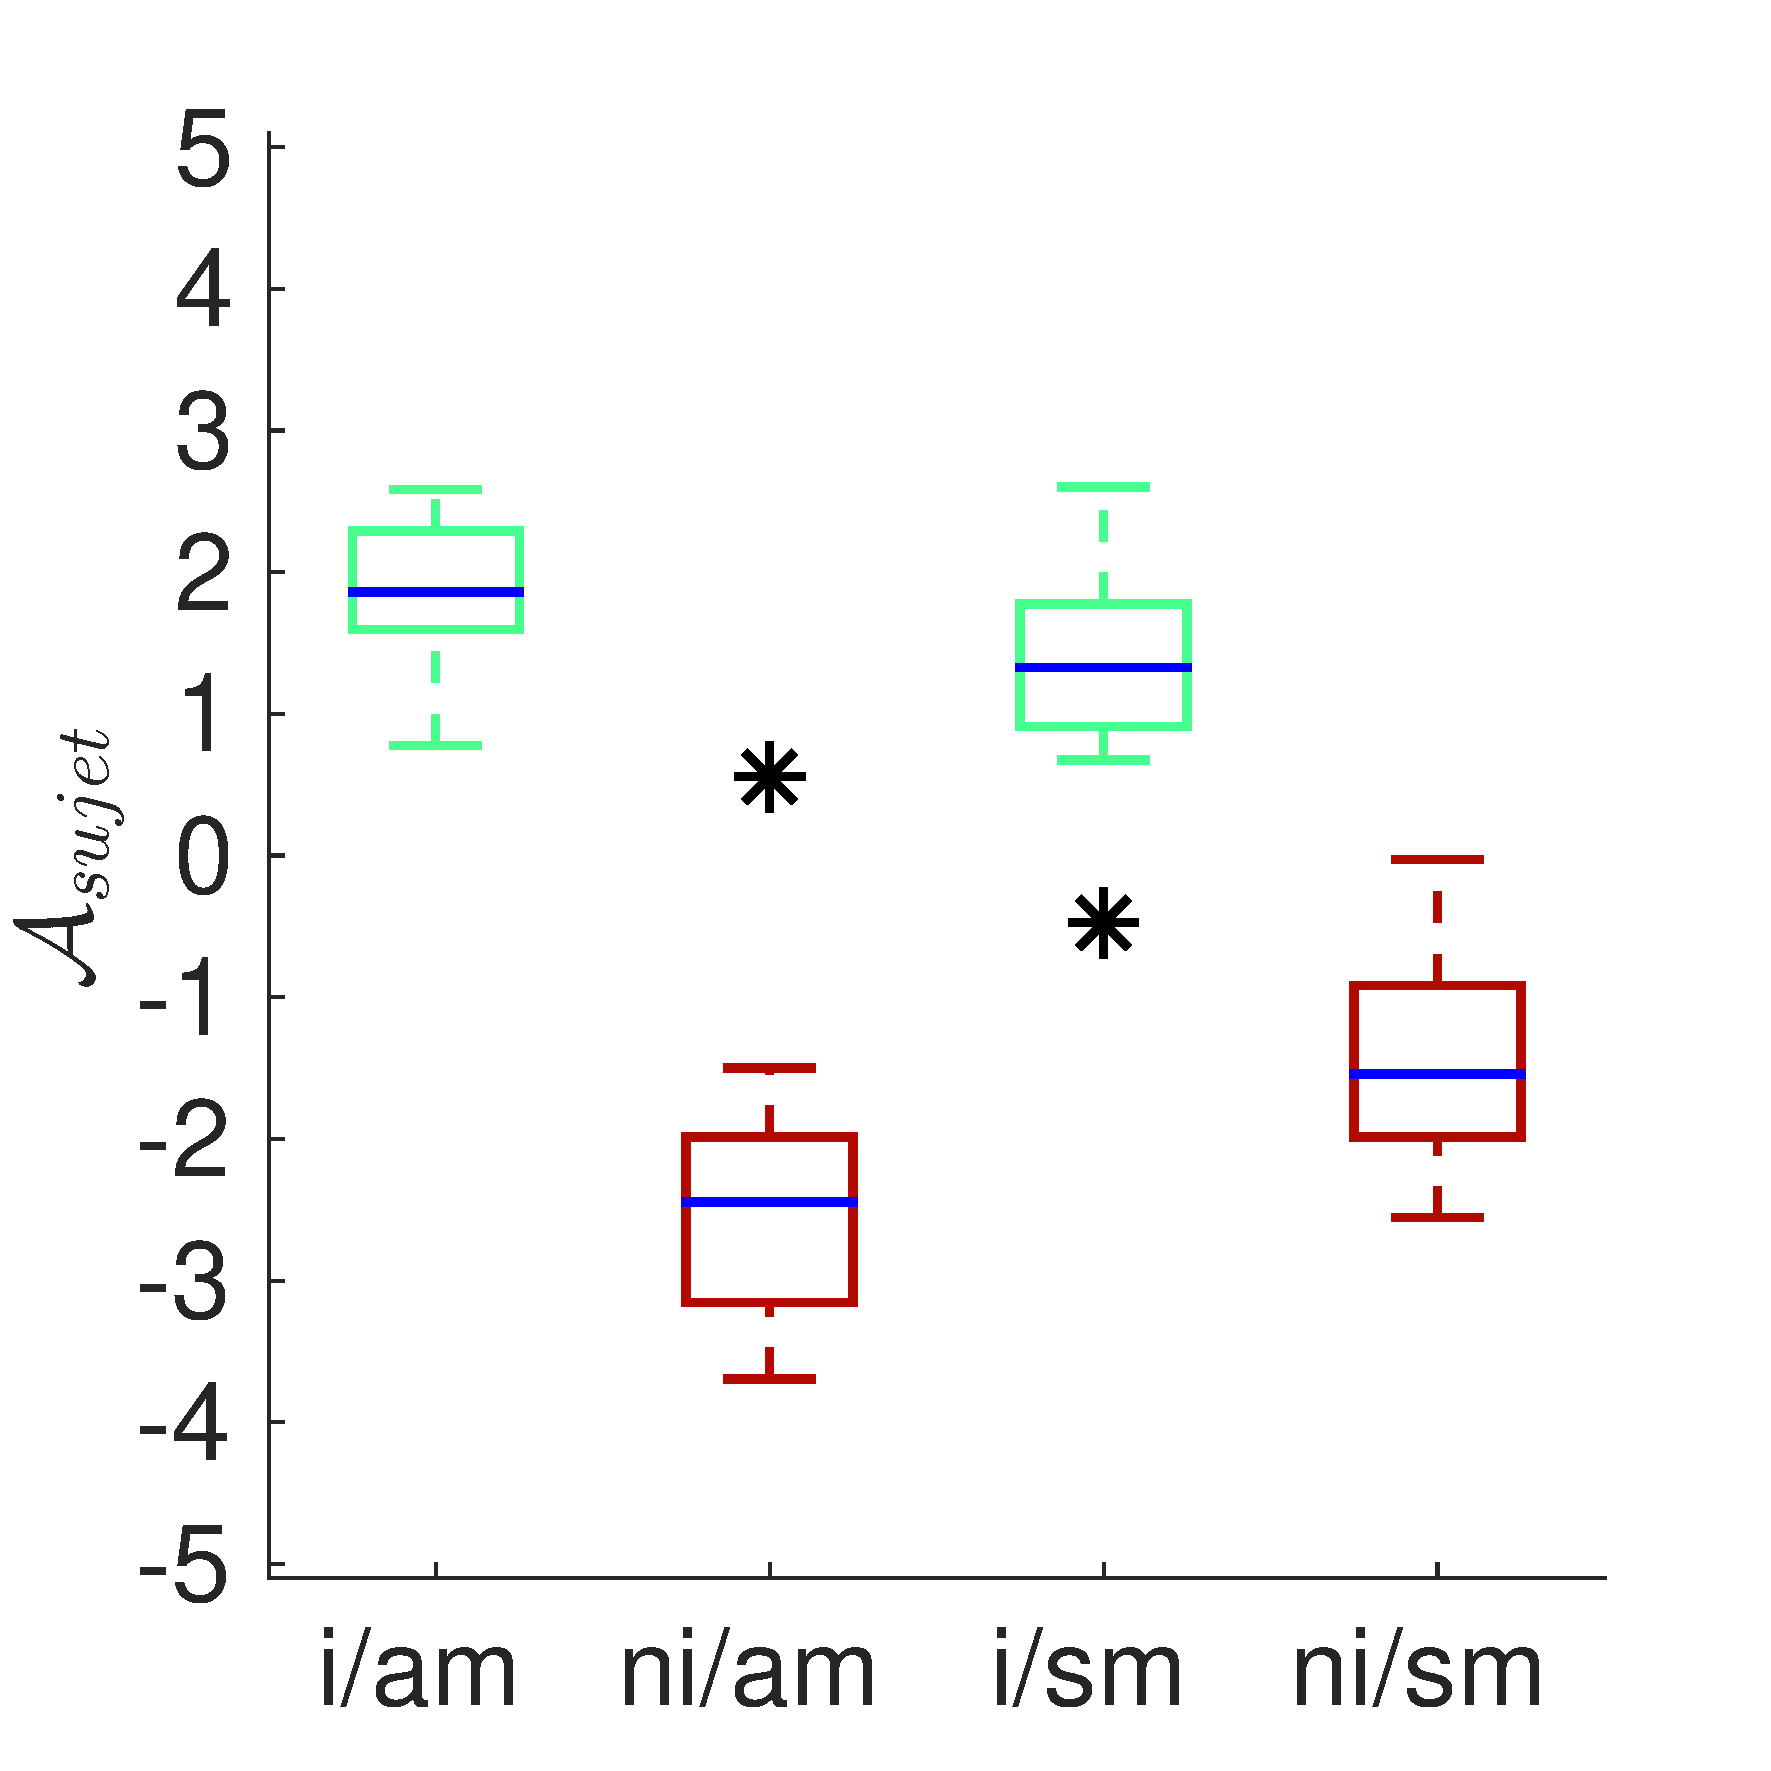
\includegraphics[width=.33\linewidth]{gfx/xp4_note_13}\label{fig:xp2_Asubject}}
        \subfloat[]
        {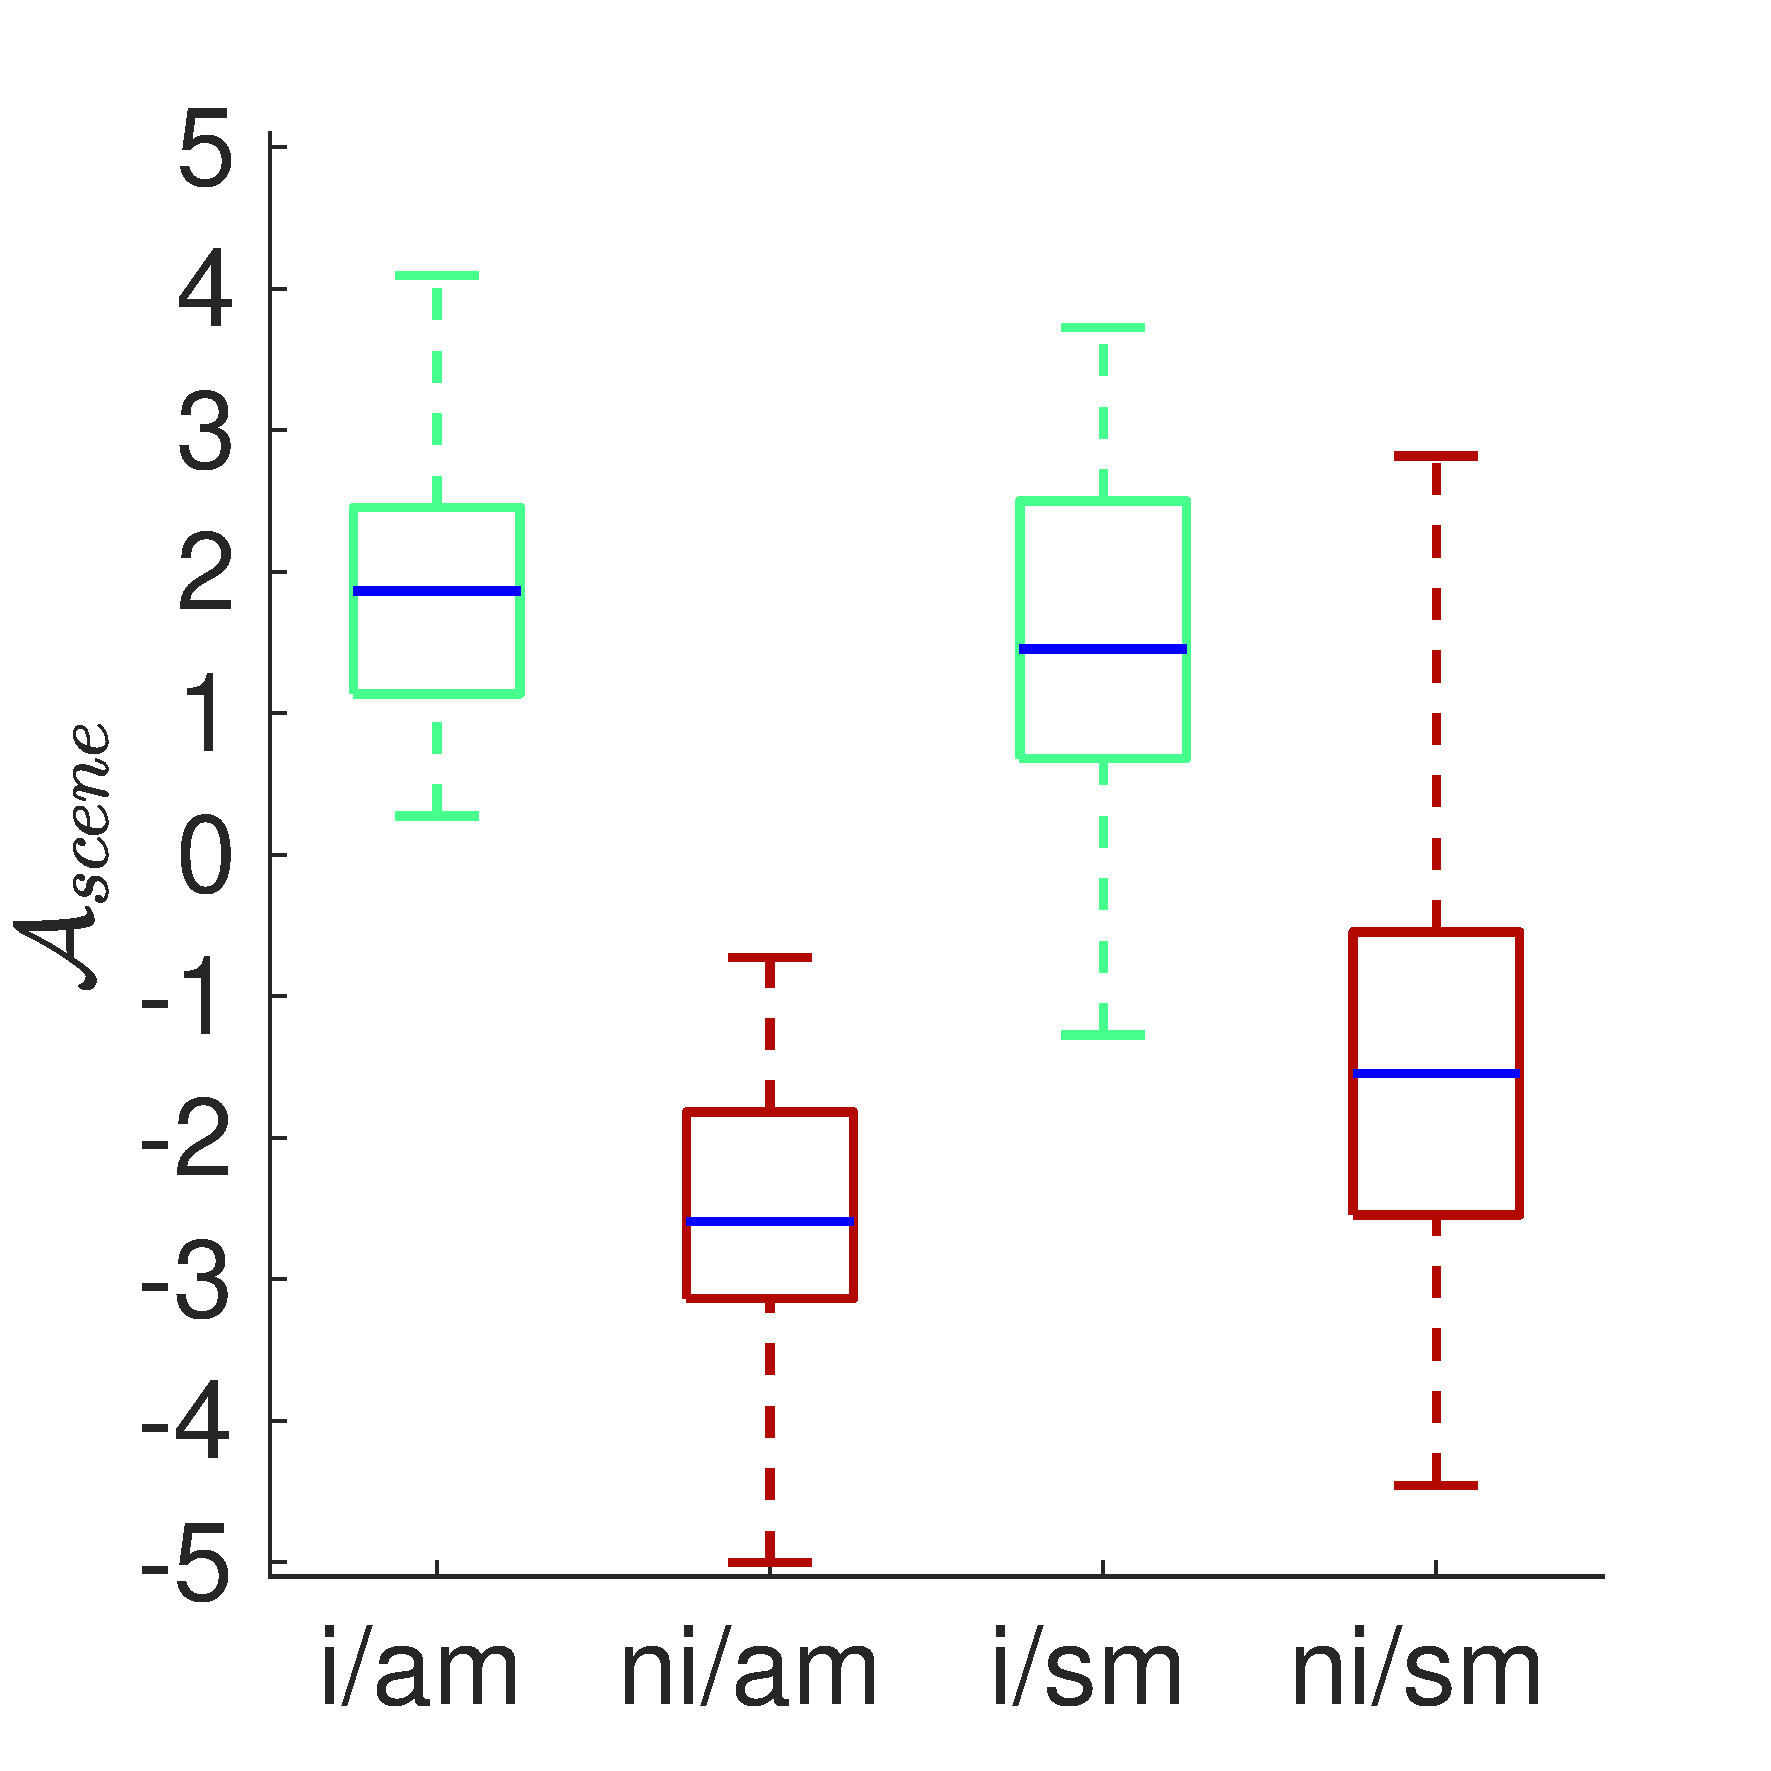
\includegraphics[width=.33\linewidth]{gfx/xp4_note_15}\label{fig:xp2_Ascene}}
        \caption{Distribution of the mean perceived pleasantness per subject $\mathcal{A}_{subject}$ (a) and the mean perceived pleasantness  per scenes$\mathcal{A}_{scene}$ (b) versus scene type. Black stars in subfigure (a) stand for the detected outlier, \ie~subject 7.}\label{fig:xp2A}
\end{figure}

%Considérons $\mathcal{A}_{sujet}$ pour les am-scènes. Il apparaît que les réponses d'un des sujets diffèrent des autres. Ce dernier a évalué positivement près de la moitié des ni/am-scènes (\cf~Annexe~\ref{app:xp2} : sujet 7). Le sujet a donné à 58\% des ni/am-scènes une note supérieure à 0, contre une moyenne de 11\% pour les autres sujets. De plus, le sujet a utilisé l'ambitus maximal (-5 à 5) pour noter à la fois les i/ et ni/am-scènes. Ces faits n'ayant pas été observés pour les autres sujets, que l'on considère les expériences 2 ou 1.b, le sujet 7 est éliminé de l'analyse.

Let us consider $\mathcal{A}_{subject}$ for the km-scenes, see Figure~\ref{fig:xp2_Asubject}. Close inspection of the answers show that one subject strongly differs from the ones of others. This subject evaluated positively close to half of the ni/km-scenes, see Annex~\ref{app:xp2}, subject 7. This subject also gave a score above 0 for 58\% of the ni/km-scenes, contrary to an average of 11\% for the remaining of the subjects.

Furthermore, this subject used the whole scale (from -5 to 5) to score both the i-scenes and the ni-scenes. Those behaviors strongly differ with the ones of the others subjects be they from this experiment or the previous ones. Subject 7 is thus discarded from the analysis.

\subsubsection{Influence of the markers on perceived pleasantness}

%Dans cette section nous étudions comment les sujets ont perçu les différents types de scènes, nommément: i/am-, ni/am-, i/sm- et ni/sm-scène. L'ANOVA à mesures répétées pratiquée sur $\mathcal{A}_{sujet}$ montre un effet significatif du type d'environnement (i/ni: $F[1,10]=175$, $p<0.01$), de la présence/absence des marqueurs (am/sm: $F[1,10]=7$, $p<0.05$), ainsi que de l'interaction entre les deux facteurs ($F[1,10]=67$, $p<0.01$).

In this section, we study the scores given by the subject while listening to the several types of scenes, namely the i/km-scenes, ni/km-scenes, i/rm-scenes and ni/rm-scenes, see Figure~\ref{fig:xp2_Ascene}. The repeated measure ANOVA applied to $\mathcal{A}_{subject}$ show a significant effect of the type environment (i/ni: $F[1,10]=175$, $p<0.01$), of the presence/absence of markers (km/rm: $F[1,10]=7$, $p<0.05$), and of the interaction between those two factors ($F[1,10]=67$, $p<0.01$).

%The \emph{post hoc} montre, quant à elle, des différences significatives entre tous les groupes d'observations, notamment entre les i/am- et i/sm-scenes ($p<0.05$) et les ni/am- et ni/sm-scenes ($p<0.01$).

The \emph{post hoc} analysis exhibits significant differences between all the groups of observations, notably between the i/km- and the i/rm scenes ($p<0.05$) as well as between the ni/km- and the ni/rm-scenes ($p<0.01$).

%Ces résultats indiquent que la suppression des événements a effectivement modifié la perception des scènes par les sujets. Nos deux hypothèses sont ainsi vérifiées:

These results indicate that the removal of the markers indeed modify the perception of the scenes by the subjects. Our two hypotheses are thus verified :

% \begin{itemize}
% \item la suppression des ni-marqueurs a amélioré les qualités perçues des ni-scènes;
% \item la suppression des i-marqueurs a diminué les qualités perçues des i-scènes.
% \end{itemize}

\begin{itemize}
\item the removal of the ni-markers improved the pleasantness of the ni-scenes;
\item the removal of the i-markers reduced the pleasantness of the i-scenes.
\end{itemize}

%L'interaction significative montre que l'effet du type d'environnement influe sur l'effet de l'absence/présence des marqueurs. En effet la moyenne des écarts entre am- et sm-scènes est plus importante pour les ni-scènes ($1.1$) que pour les i-scènes ($0.5$).

The significant interaction shows that the effect of the type of environment influences the effect of the presence/absence of the markers. Indeed, the average of the differences between km-scenes and rm-scenes is larger for the ni-scenes ($1.1$) than for the i-scenes ($0.5$).

\subsection{Discussion}

%Cette expérience fait apparaître que la présence, dans une scène, des marqueurs relevés à l'expérience 1 impacte bien l'agrément perçu. La suppression des ni-marqueurs a un effet bénéfique sur le ressenti des ni-scènes, tandis que, plus surprenant, la suppression des i-marqueurs dégrade légèrement la qualité des i-scènes. Ce dernier point est d'autant plus marquant que, du fait de la suppression des marqueurs, le niveau des i/am-scènes est supérieur à celui des i/sm-scènes.

This experiment shows that the presence of markers identified during the analysis of experiment 1 does have an impact on the perceived pleasantness. The removal of the ni-markers has a positive effect on the perception of the ni-scenes. Perhaps more surprisingly the removal of the i-markers slightly decreases the perception of the i-scenes. This is even more striking because, due to the removal of the markers, the acoustic pressure level of the i/km-scenes is higher than the one of the i/rm-scenes.

%Les i-marqueurs ont donc bien un effet bénéfique sur la perception d'un environnement. Le fait que leur suppression diminue $\mathcal{A}_{scene}$ montre clairement qu'il est possible d'améliorer la qualité sonore d'un lieu en ajoutant des sons bien acceptés comme \emph{oiseau}. Ces conclusions vont dans le sens de l'approche positive introduite par Schafer \cite{schafer1977tuning}.

The i-markers do have a positive impact on the perception of an environment. The fact that their removal decreases $\mathcal{A}_{scene}$ indicate that it should possible to improve the perceived pleasantness of a given urban area by the addition of sounds commonly considered as pleasant such as \emph{bird calls}. Those conclusions are in line with the positive approach introduced by Schafer in \cite{schafer1977tuning}.

%%%%%%%%%%%%%%%%%%%%%%%%%%%%%%%%%%%%%%%%%%%%%%%%%%%%%%%%%%%%
%%%%%%%%    DISCUSSION AND PERSPECTIVES   %%%%%%%%%%%%%%%%%%
%%%%%%%%%%%%%%%%%%%%%%%%%%%%%%%%%%%%%%%%%%%%%%%%%%%%%%%%%%%%


\section{Outcomes for soundscape perception}
\label{sec:conclusion}
%Les expériences ont montré que la majorité des descripteurs utilisés, qu'ils soient sémantiques ou structurels, permettent de faire la distinction entre une scène idéale et une scène non-idéale.

This series of three experiments showed that most of the descriptors used in this study, be they semantic or based on acousitc level, allows us to distinguish between an ideal scene and a non ideal one.

%Cependant, nous observons que les caractéristiques physiques corrélées à l'agrément diffèrent clairement suivant le type de scènes. Dans le cas des scènes idéales, c'est avant tout l'émergence de marqueurs sonores qui détermine la qualité perçue, alors que dans le cas des scènes non-idéales, c'est le niveau sonore global qui influe sur l'agrément.

That being said, we observe that the physical characteristics correlated with the perceived pleasantness clearly differ depending on the type of scenes. In the case of ideal scenes, it is above all the emergence of sound markers that determines the perceived quality, whereas in the case of non-ideal scenes, it is the overall sound level that prominently influences the perceived quality.

%Ces résultats tendent à confirmer que la perception des qualités d'une scène dépend avant tout des sources sonores qui la composent, les caractéristiques structurelles mobilisées dans le processus perceptif semblant varier d'une source à l'autre, et d'un type d'environnement à l'autre. Ce fait montre qu'il est illusoire d'envisager qu'un descripteur physique holistique puisse rendre compte, de manière pertinente, des qualités affectives de tous types d'environnement.

These results show that the perception of the qualities of a scene indeed depends primarily on its sound sources which are identified. The characteristics that are taken into account during the perceptual process appear to vary from one source to the other, from one type of environment to the other. This fact leads the authors to believe that there is little hope to find a holistic physical descriptor that can adequately account for the affective qualities of all types of sound environment.

%Cet état de fait peut potentiellement influer sur les stratégies à adopter pour améliorer la qualité de l’environnement sonore:

Those results may have an impact on the relevant strategies to adopt while trying to improve the quality of a sound environment:

% \begin{itemize}
% \item dans le cadre de scènes non-idéales, il s'agit de diminuer le niveau sonore, soit de manière globale, soit en agissant sur certaines sources (\emph{sirène}, \emph{klaxon});
% \item dans le cadre de scènes idéales, il s'agit 1) d'identifier les sons agréables, \ie~les marqueurs sonores, 2) de baisser le niveau des autres sons, 3) voire, en restant dans la limite du raisonnable, d'augmenter le niveau des marqueurs par rapport aux autres sons.
% \end{itemize}

\begin{itemize}
\item in the case of non ideal scenes, one should focus on reducing the acoustic pressure level, whether globally, or by discarding specific sources such as \emph{sirens} or \emph{car horns}
\item in the case of ideal scenes, one should first identify which sources are pleasant to the targeted community, second lower the volume of the other sound sources, and, if possible, raise the contribution or add positive sound markers.
\end{itemize}

%Ces travaux nous permettent enfin de conjecturer quant à la nature des représentations mentales des concepts «~environnement sonore urbain agréable~» (EA) et «~environnement sonore urbain désagréable~» (ED).

Finally, these works allow us to conjecture as to the nature of the mental representations of the concepts "pleasant (urban sound) environment" (PE) and "unpleasant (urban sound) environment" (UE).

%Premièrement, le fait que les informations sémantiques (sources sonores présentes) et structurelles soient différentes pour les scènes idéales et non-idéales nous porte à croire que ces deux types d'informations caractérisent les concepts EA et ED.

First, the fact that the semantic information (which sound source is present) and compositional information (at which level) are different for ideal and non-ideal scenes leads us to believe that these two types of information characterize the PE and UE concepts.

%Deuxièmement, le fait que la suppression des marqueurs sonores modifie l'agrément perçu nous porte à croire que le concept abstrait lié à l'agrément (\eg. scène agréable) dépend de l'activation d'un réseau de concepts concrets liés aux sources (dans notre cas \emph{oiseau}, \emph{cloche} et \emph{sonnette vélo}).

Secondly, the fact that the removal of sound markers changes the perceived pleasantness leads us to believe that the abstract concept related to pleasantness depends on the activation of a network of concepts strongly linked to the sources which are in the case of this study: \emph{bird}, \emph{church bell} and \emph{bicycle bell}.

%Troisièmement, le fait que les descripteurs structurels corrélés à l'agrément diffèrent en fonction du type de scènes nous porte à croire que les caractéristiques structurelles permettant de distinguer deux instances d'un même concept abstrait lié à l'agrément ne sont pas les mêmes pour EA et ED.

%Third, the fact that the compositional descriptors correlated with the perceived pleasantness change according to the type of scenes leads us to believe that the compositional characteristics that allow us to distinguish between two instances of the same abstract concept linked to the pleasantness are not the same for PE and UE.

\section{Conclusion}

%Au terme de notre étude, nous pensons que la simulation est un outil dont le développement pourrait permettre aux décideurs en matière d'urbanisme d'interroger toute une communauté sur ses représentations propres des environnements sonores auxquels elle est exposée, et, pourquoi pas, sur les représentations des environnements sonores auxquels elle voudrait être exposée.

The outcomes of the three experiments described in this paper demonstrate the usefulness of considering a dedicated simulation tool such as \emph{simScene} in order to scientifically question the perception of soundscapes in an innovative way. We also believe that its wider usage could enable urban planning decision-makers to question an entire community about its own representations of the sound environment to which they are exposed, and about the representations of the sound environments to which they would like to be exposed to.

%Dans la continuité des travaux réalisés, il conviendrait de multiplier les expériences de simulation, en faisant varier les qualités affectives (calme, confortable, gênante, \etc), mais aussi en spécifiant des lieux particuliers (parc, place, rue, \etc), afin d'élaborer des corpus entiers de scènes cognitivement renseignées de paysages sonores.

Future work should consider several other simulation experiments by changing the emotional qualities (quiet, comfortable, troublesome, etc.), but also by specifying specific urban locations (park, square, street, etc.), in order to provide to the scientific community an entire corpora of cognitively informed soundscapes.

%Il serait par ailleurs intéressant d'utiliser la simulation afin d'étudier plus avant les effets provoqués par la modification volontaire d'une caractéristique d'une scène, comme lors de la suppression des marqueurs sonores pratiquée dans l'expérience 2.

It would also be interesting to use the alteration capabilities of the proposed paradigm in order to study further the effects caused by the voluntary modification of a characteristic of a scene, as during the suppression of the sound markers practiced in experiment 2.

%Une des pistes privilégiée dans ce cadre serait d'étudier l'impact de l'ajout de marqueurs sonores positivement appréciés à une scène non idéal pour étudier l'hypothèse que ce type d'ajout améliorerait la qualité perçue de la scène.

One interesting avenue in this direction would be to study the impact of adding positively appreciated sound markers to a non ideal scene in order to study the hypothesis that this type of addition would improve the perceived quality of the scene.

%Enfin, l'on pourrait encore étudier l'influence des contextes socio-culturels sur la perception. Dans les faits, si le son de cloche est le plus souvent un marqueur d'environnement de qualité pour un occidental, cela ne se vérifie pas nécessairement auprès de sujets de culture orientale, moyen-orientale ou autre.

Finally, one should study the influence of socio-cultural contexts on perception. Indeed, if the sound of the church bell is most often a quality environment marker for a Westerner. This do not necessarily hold true for subjects of Eastern, Middle Eastern or other cultures.

%Outre les possibilités déjà évoquées, le protocole de simulation présenté ici ainsi que son implémentation apporte encore dans ce cas deux avantages:

Once again, besides the interesting possibilities already mentioned, the simulation protocol presented here as well as its implementation brings in this case two important advantages:

%\begin{itemize}
% \item le simulateur peut être déployé à large échelle via internet du fait de l'architecture logicielle choisie pour son développement;
% \item les scènes simulées peuvent être analysées sans avoir à tenir compte des différentes langues maternelles des sujets, la nature sémantique des classes de sons utilisées étant connue \emph{a priori} par l'expérimentateur et sans avoir besoin d'analyser la scène sonore pour idientifier les sources, leurs présences dans la scène étant directement exploitable.
% \end{itemize}

\begin{itemize}
\item The simulator can be deployed on a large scale via the Internet thanks to the web-based software architecture;
\item simulated scenes can be analyzed without the need to take into account the different mother tongues of the subjects, the semantic nature of the classes of sounds used being known \emph{a priori} by the experimenter and without the need to analyze and annotate the sound scene to identify the sources, their occurrences in the simulated scene being directly available.
\end{itemize}

%Bien évidemment, ces approches nécessitent d'accroître la taille des banques de sons isolés disponibles, un effort conséquent, mais nécessaire, qui contribuera grandement aux nombreux domaines de recherche ayant trait aux scènes sonores.

%\nm{a ce propos, il n'est pas fait mention des sons manquants pour les subjects (cf. protocole expe de 1a);
%ne faudrait -il pas en dire 2 mots ce qui alimenterait aussi la discussion sur la dependance de la qualite (et l'efficacite) de la simulation a  la constitution de la base de donnees de textures et d'evenemetns ?}

\section*{\normalsize Acknowledgements}
\setlength{\parindent}{0.7cm}
Research project partly funded by ANR-11-JS03-005-01. The authors would like to thank the students of the Ecole Centrale de Nantes for their willing participation.


%%%%%%%%%%%%%%%%%%%%%%%%%%%%%%%%%%%%%%%%%%%%%%%%%%%%%%%%%%%%
%%%%%%%%%%%%%%%%    Bibliography    %%%%%%%%%%%%%%%%%%%%%%%%
%%%%%%%%%%%%%%%%%%%%%%%%%%%%%%%%%%%%%%%%%%%%%%%%%%%%%%%%%%%%

\bibliographystyle{elsarticle-num}
\bibliography{Bibliography}

%%%%%%%%%%%%%%%%%%%%%%%%%%%%%%%%%%%%%%%%%%%%%%%%%%%%%%%%%%%%
%%%%%%%%%%%%%%%%%%%    APPENDICES   %%%%%%%%%%%%%%%%%%%%%%%%
%%%%%%%%%%%%%%%%%%%%%%%%%%%%%%%%%%%%%%%%%%%%%%%%%%%%%%%%%%%%

\appendix
\newpage
\section{Taxonomy of sound classes}
\label{app:taxonomie}

\begin{figure}[!hp]
    \centering
        {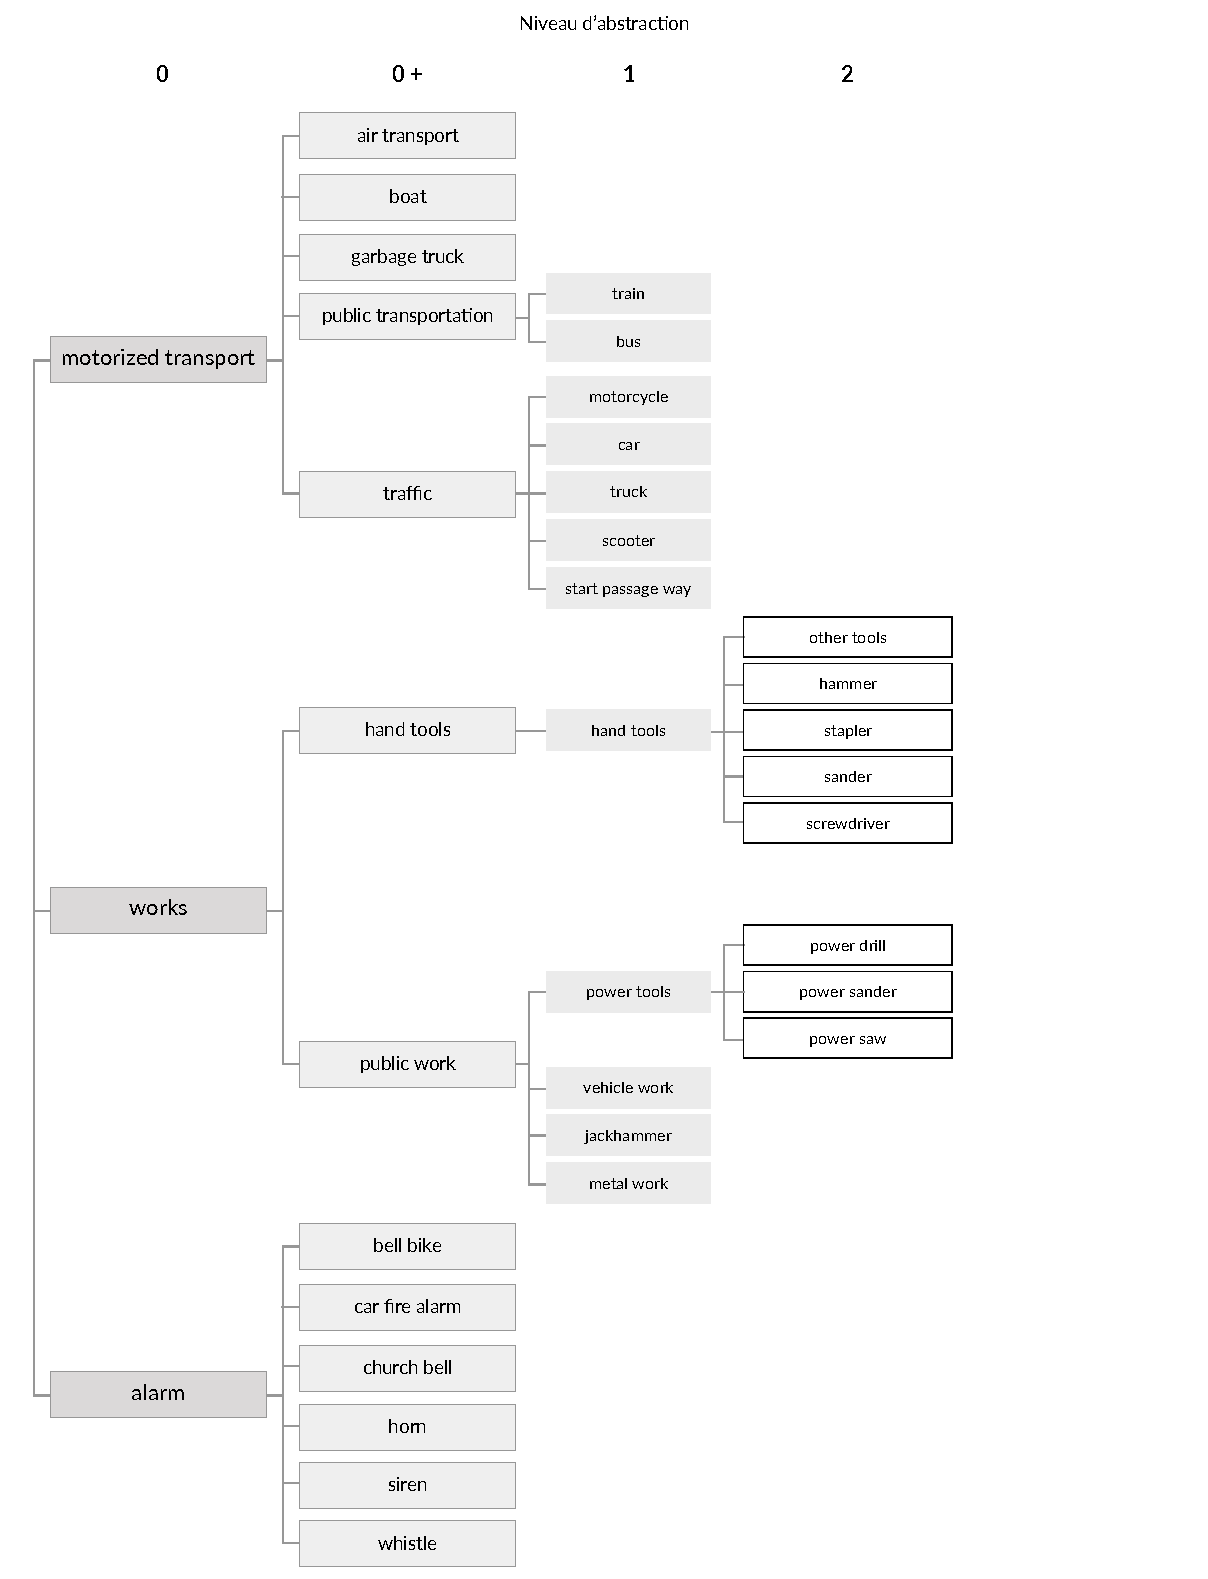
\includegraphics[trim={ 0 0 0cm 1cm},clip,width=.9\columnwidth]{gfx/appendix/event_1_en}\label{fig:taxonomieEventa}} \par
         \caption{Taxonomy of sound classes of mechanical events used for the simulation urban soundscapes  with level of abstraction from left to right.}
       \label{fig:taxonomieEa}
\end{figure}

\begin{figure}[hp]
    \centering
        {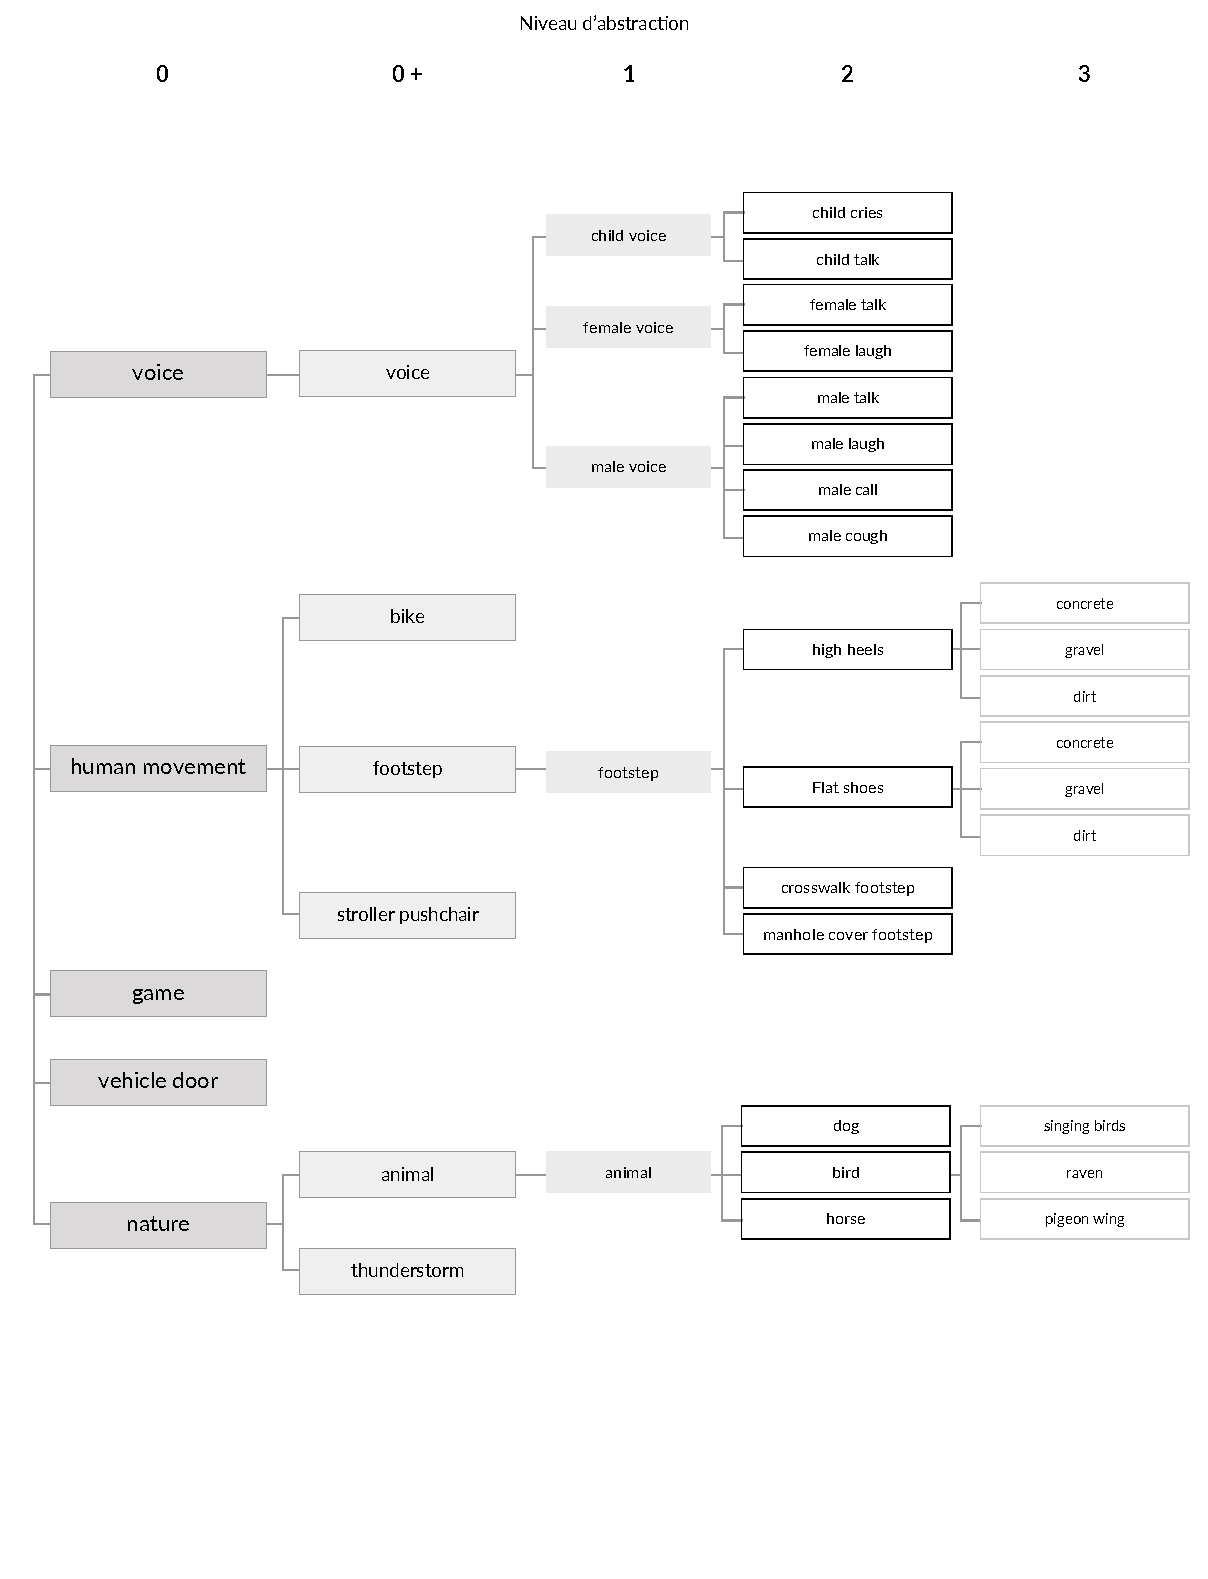
\includegraphics[trim={ 0 0 0cm 1cm},clip,width=.9\columnwidth]{gfx/appendix/event_2_en}\label{fig:taxonomieEventb}}
       \caption{Taxonomy of sound classes of non-mechanical events used for the simulation urban soundscapes with level of abstraction from left to right.}
       \label{fig:taxonomieEb}
\end{figure}

\begin{figure}[hp]
  \centering
        {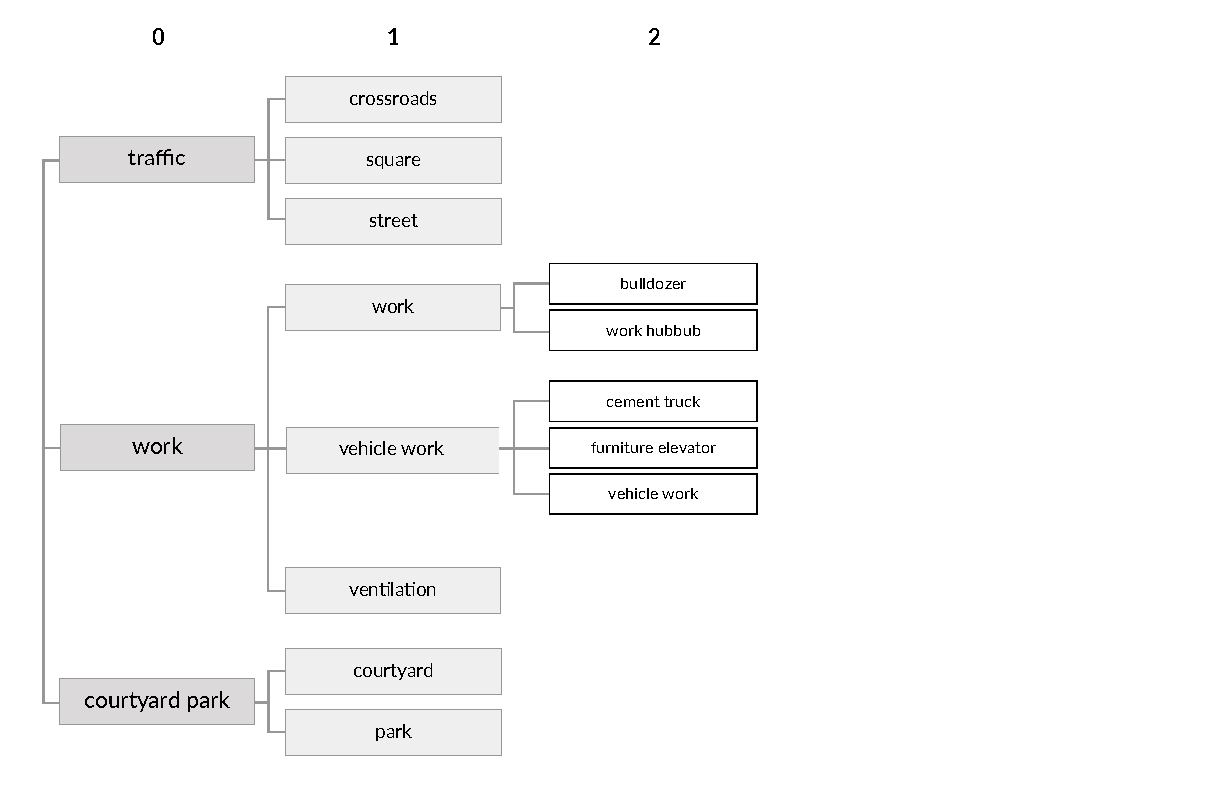
\includegraphics[trim={ 0 0 7cm 0},clip,width=.7\columnwidth]{gfx/appendix/texture_1_en}\label{fig:taxonomieTexturea}} \par

        {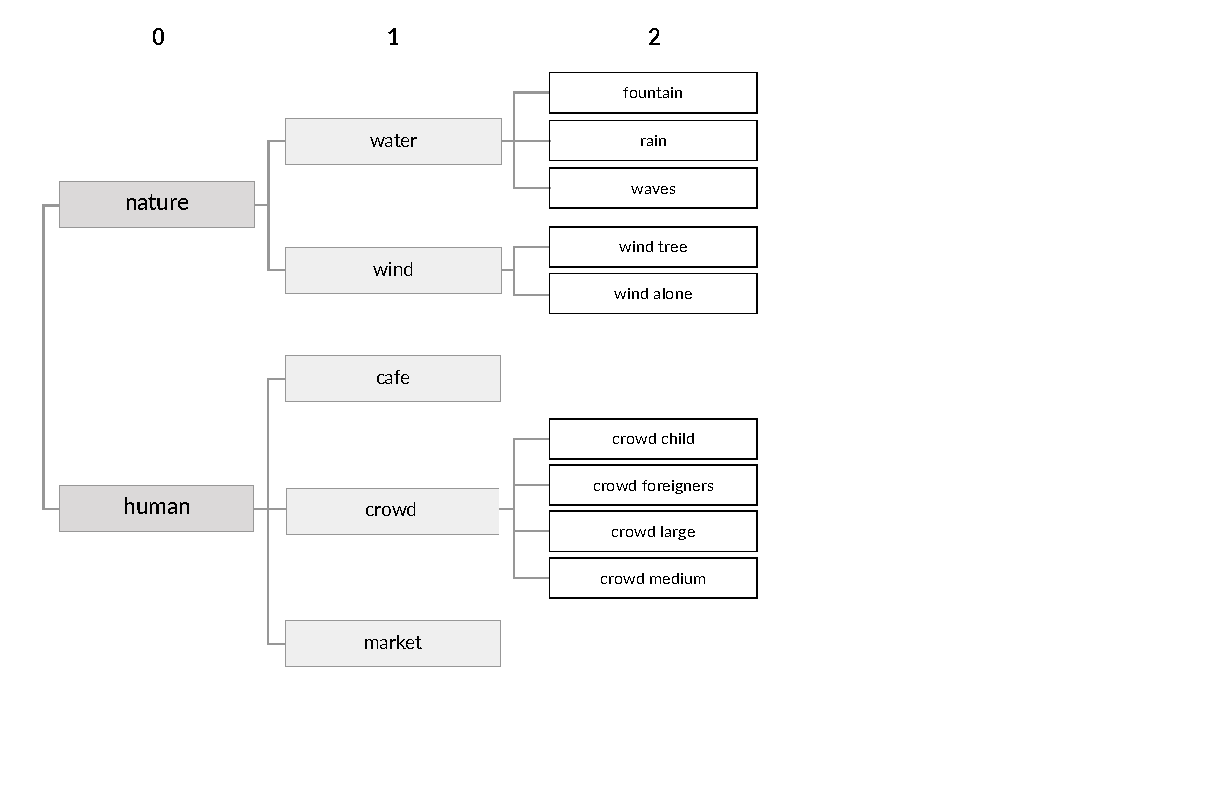
\includegraphics[trim={ 0 0 7cm 1cm},clip,width=.7\columnwidth]{gfx/appendix/texture_2_en}\label{fig:taxonomieTextureb}}
       \caption{Taxonomy of sound classes of textures used for the simulation urban soundscapes with level of abstraction from left to right.}
       \label{fig:taxonomieT}
\end{figure}

\newpage
\section{Distribution of pleasantness scores given by the subjects during experiment 2}
\label{app:xp2}

\begin{figure}[h]
        \myfloatalign
        \subfloat[subject 1]
        {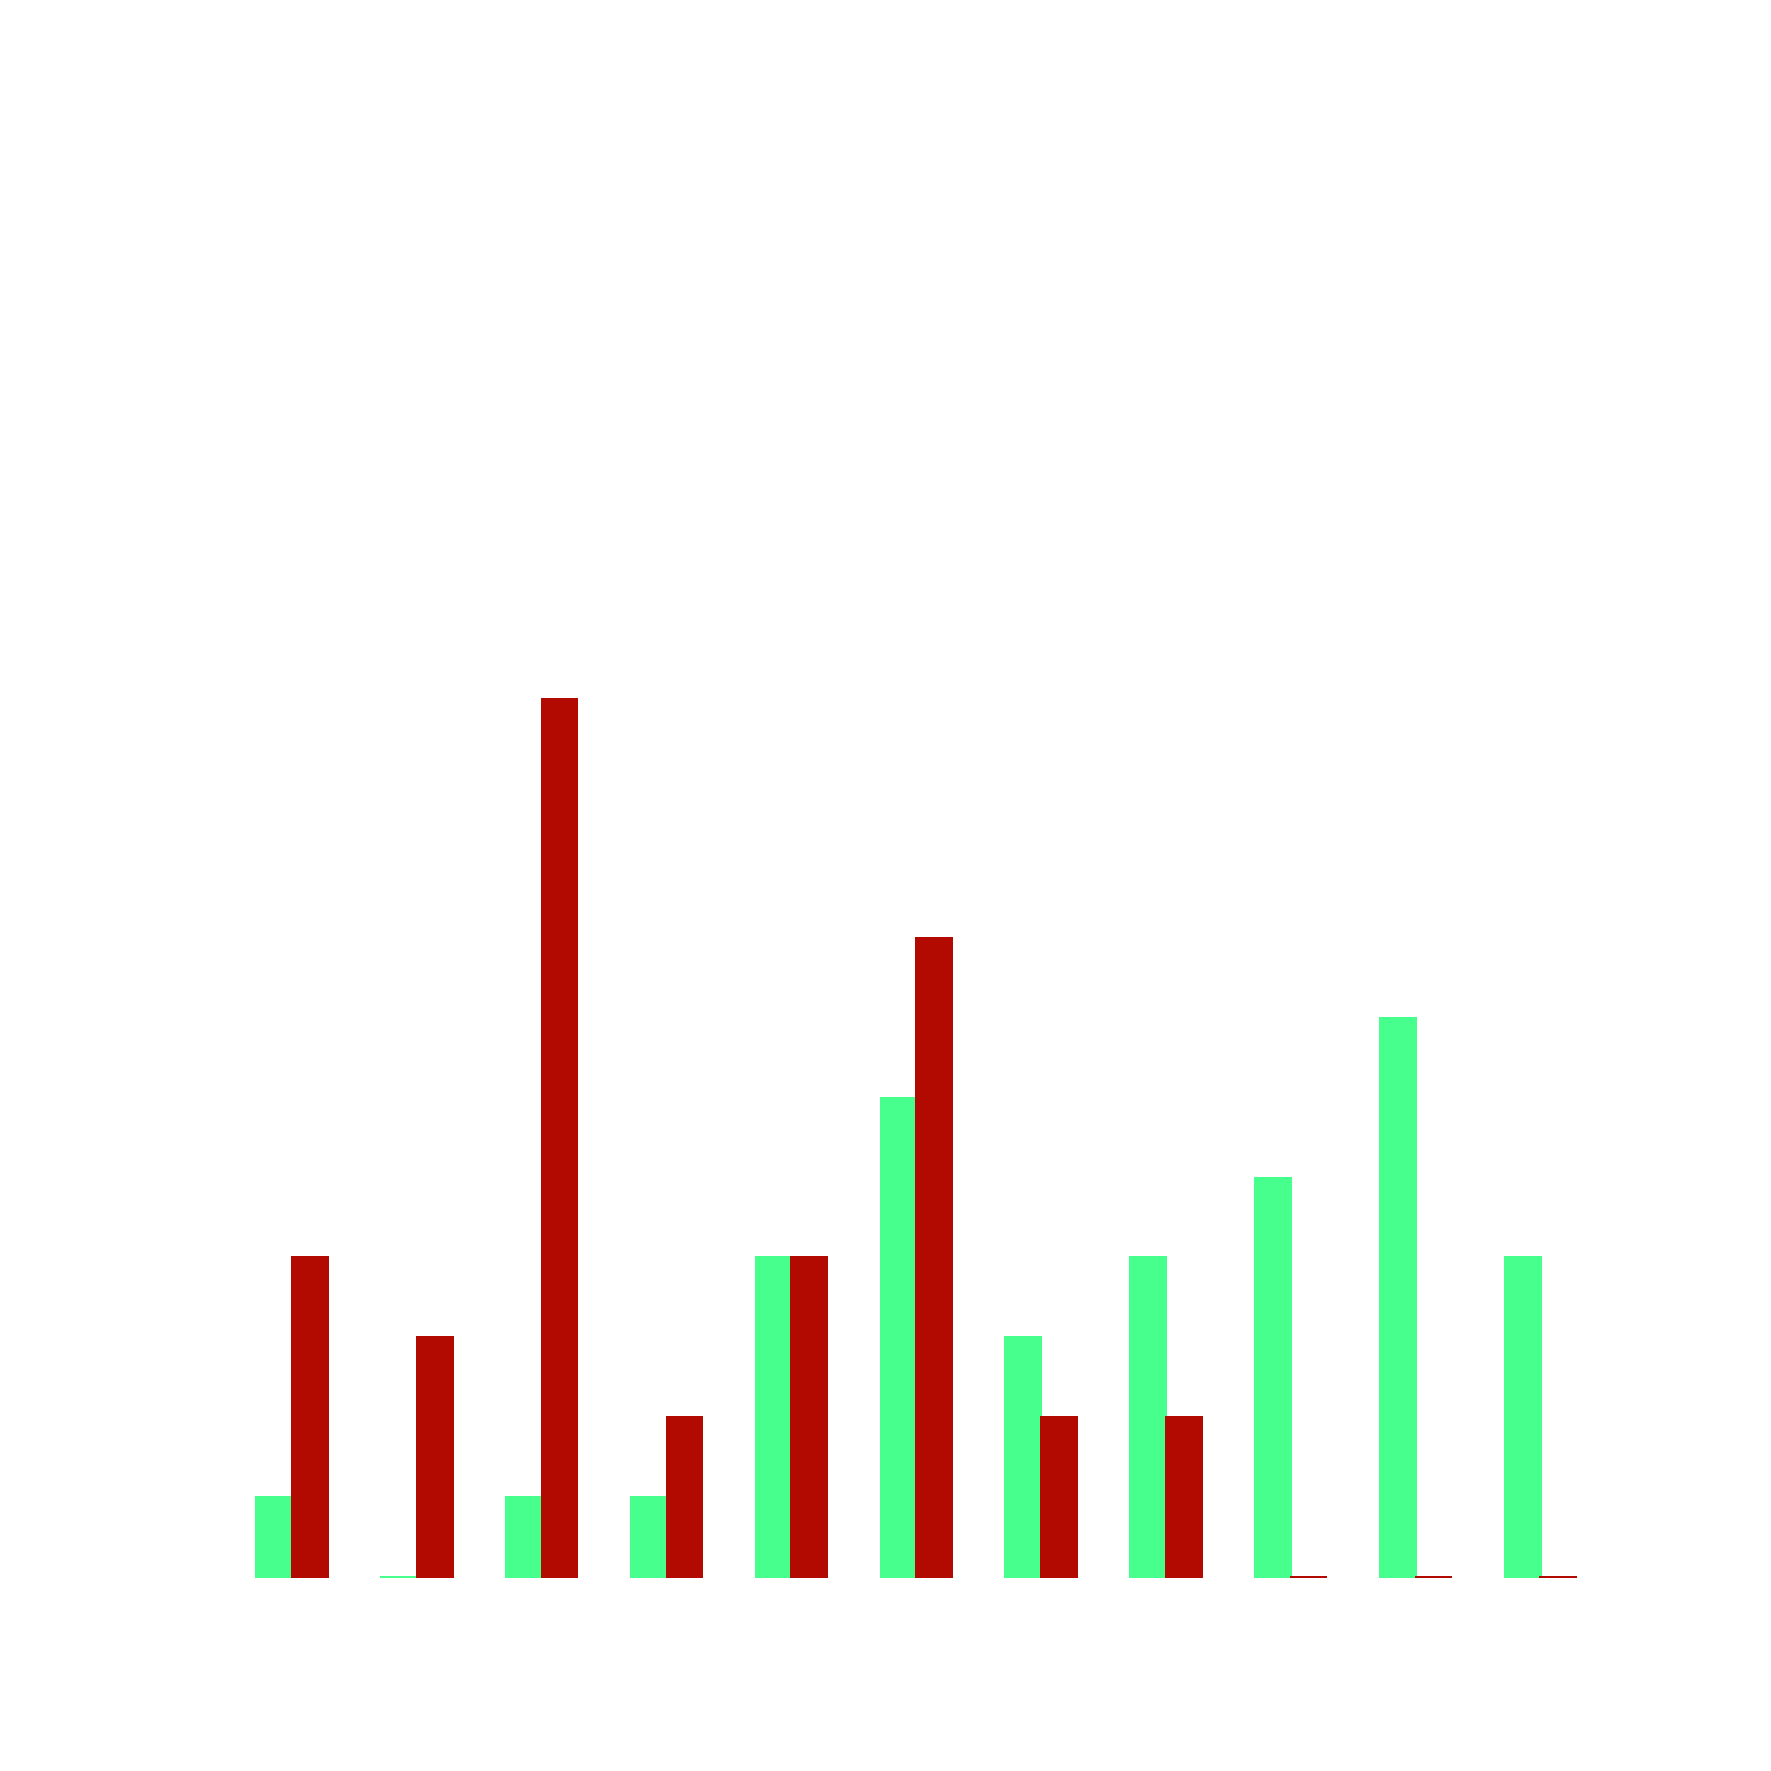
\includegraphics[width=.24\linewidth]{gfx/appendix/xp4_note_1}\label{fig:xp4_note_1a}}
        \subfloat[subject 2]
        {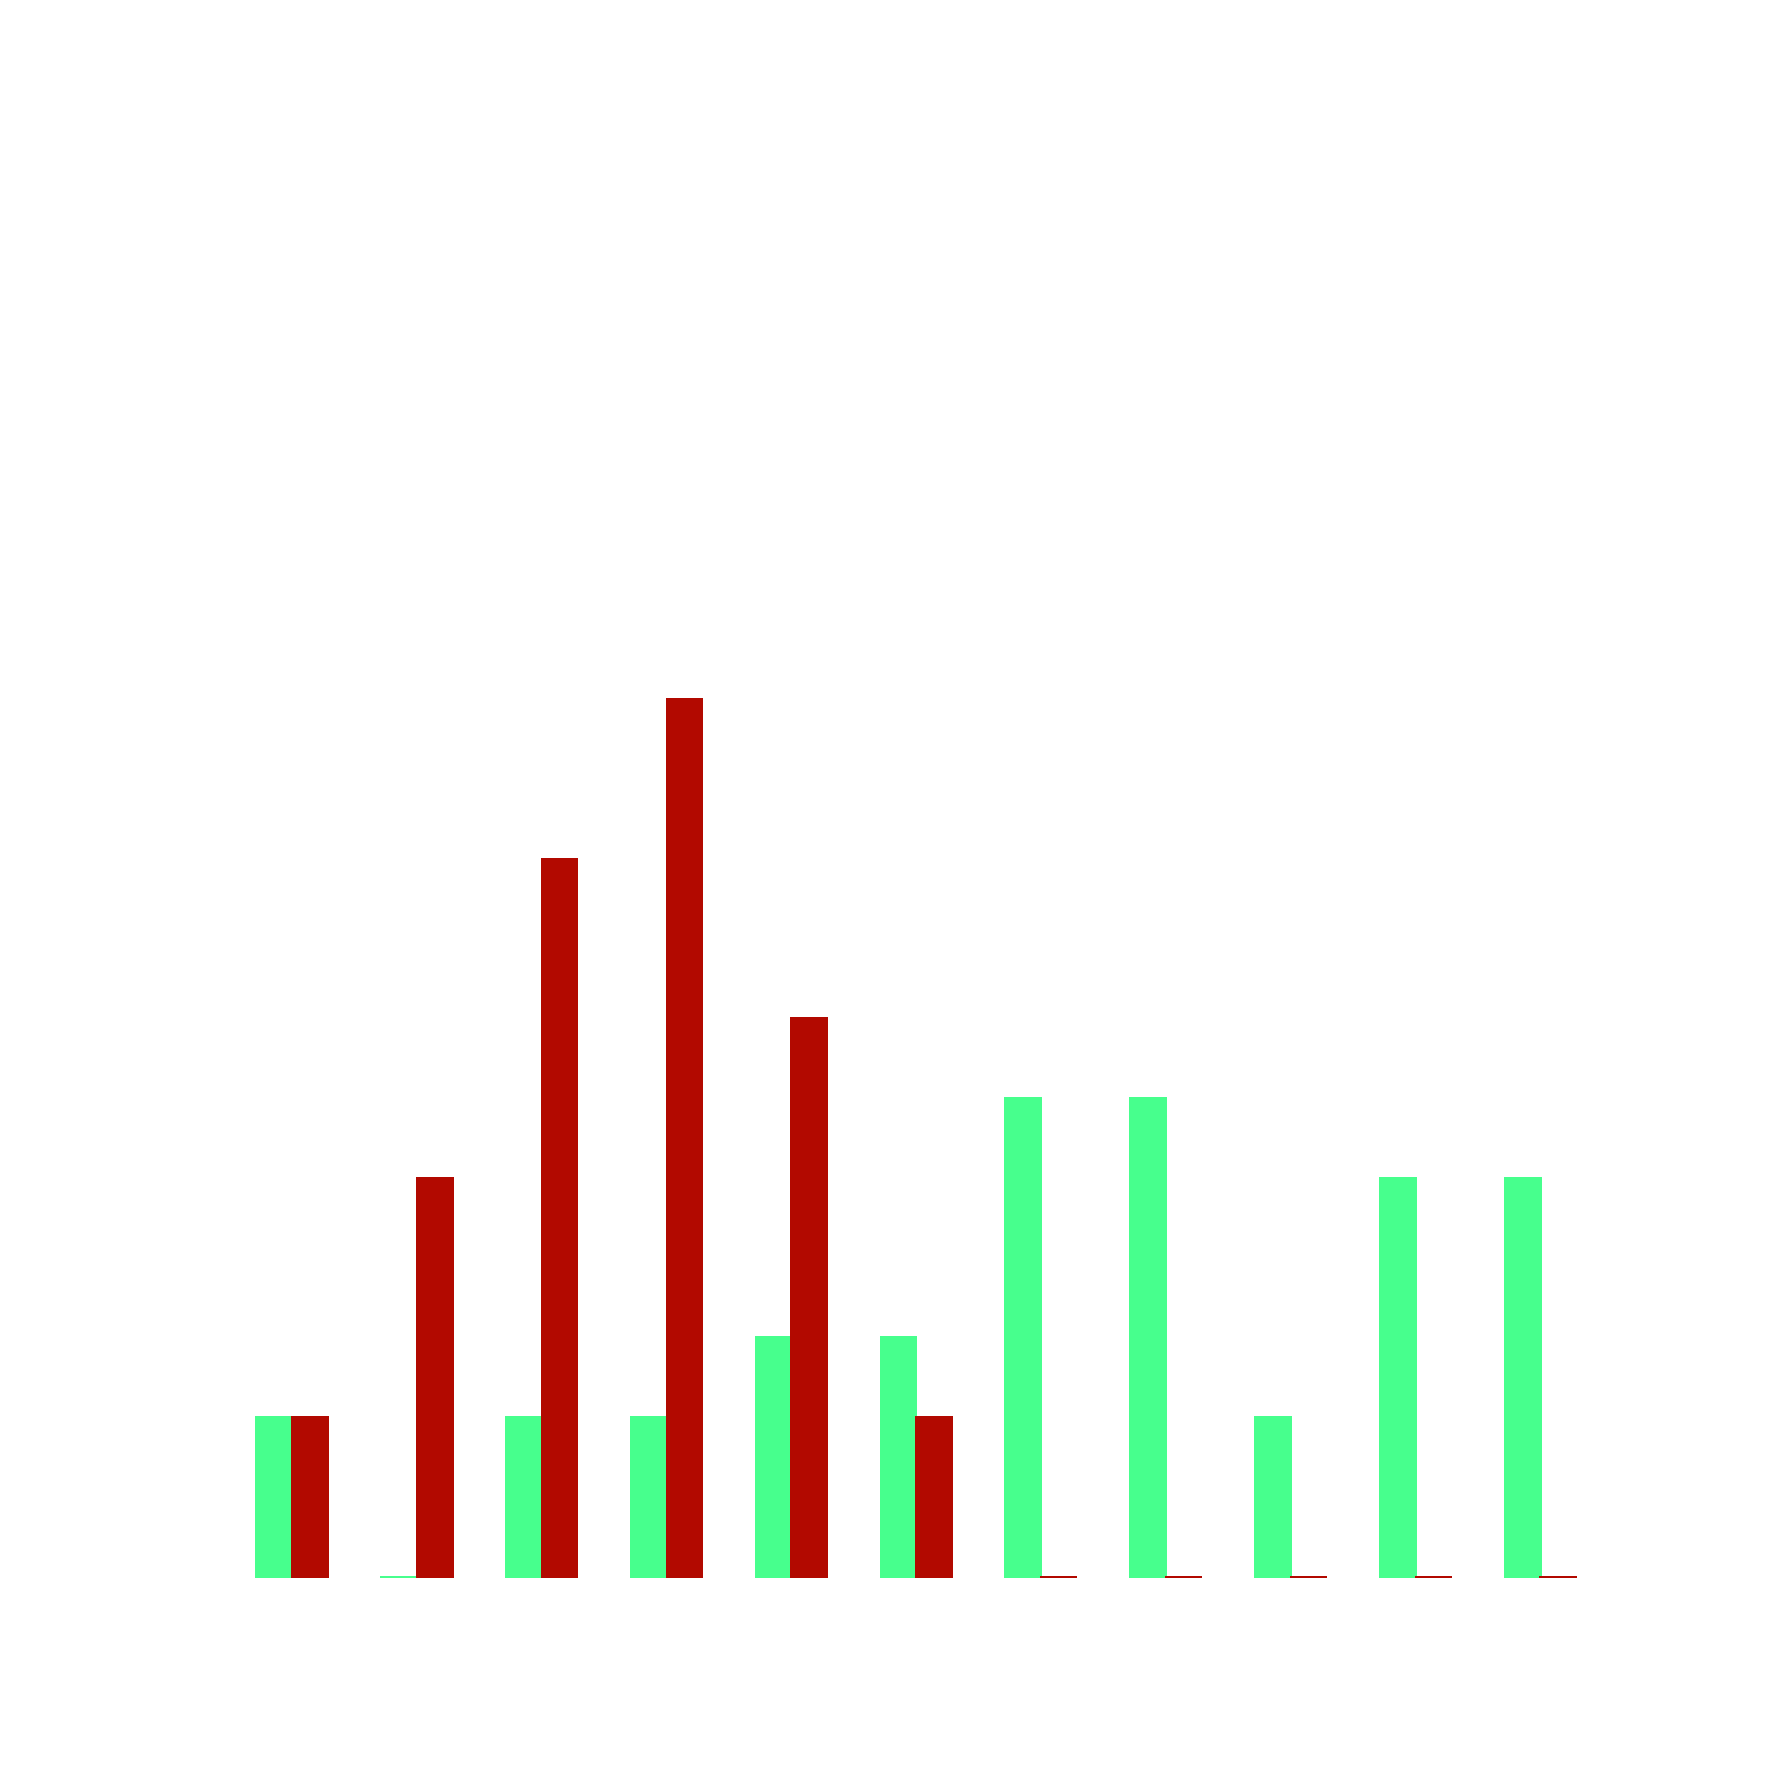
\includegraphics[width=.24\linewidth]{gfx/appendix/xp4_note_2}\label{fig:xp4_note_1b}}
        \subfloat[subject 3]
        {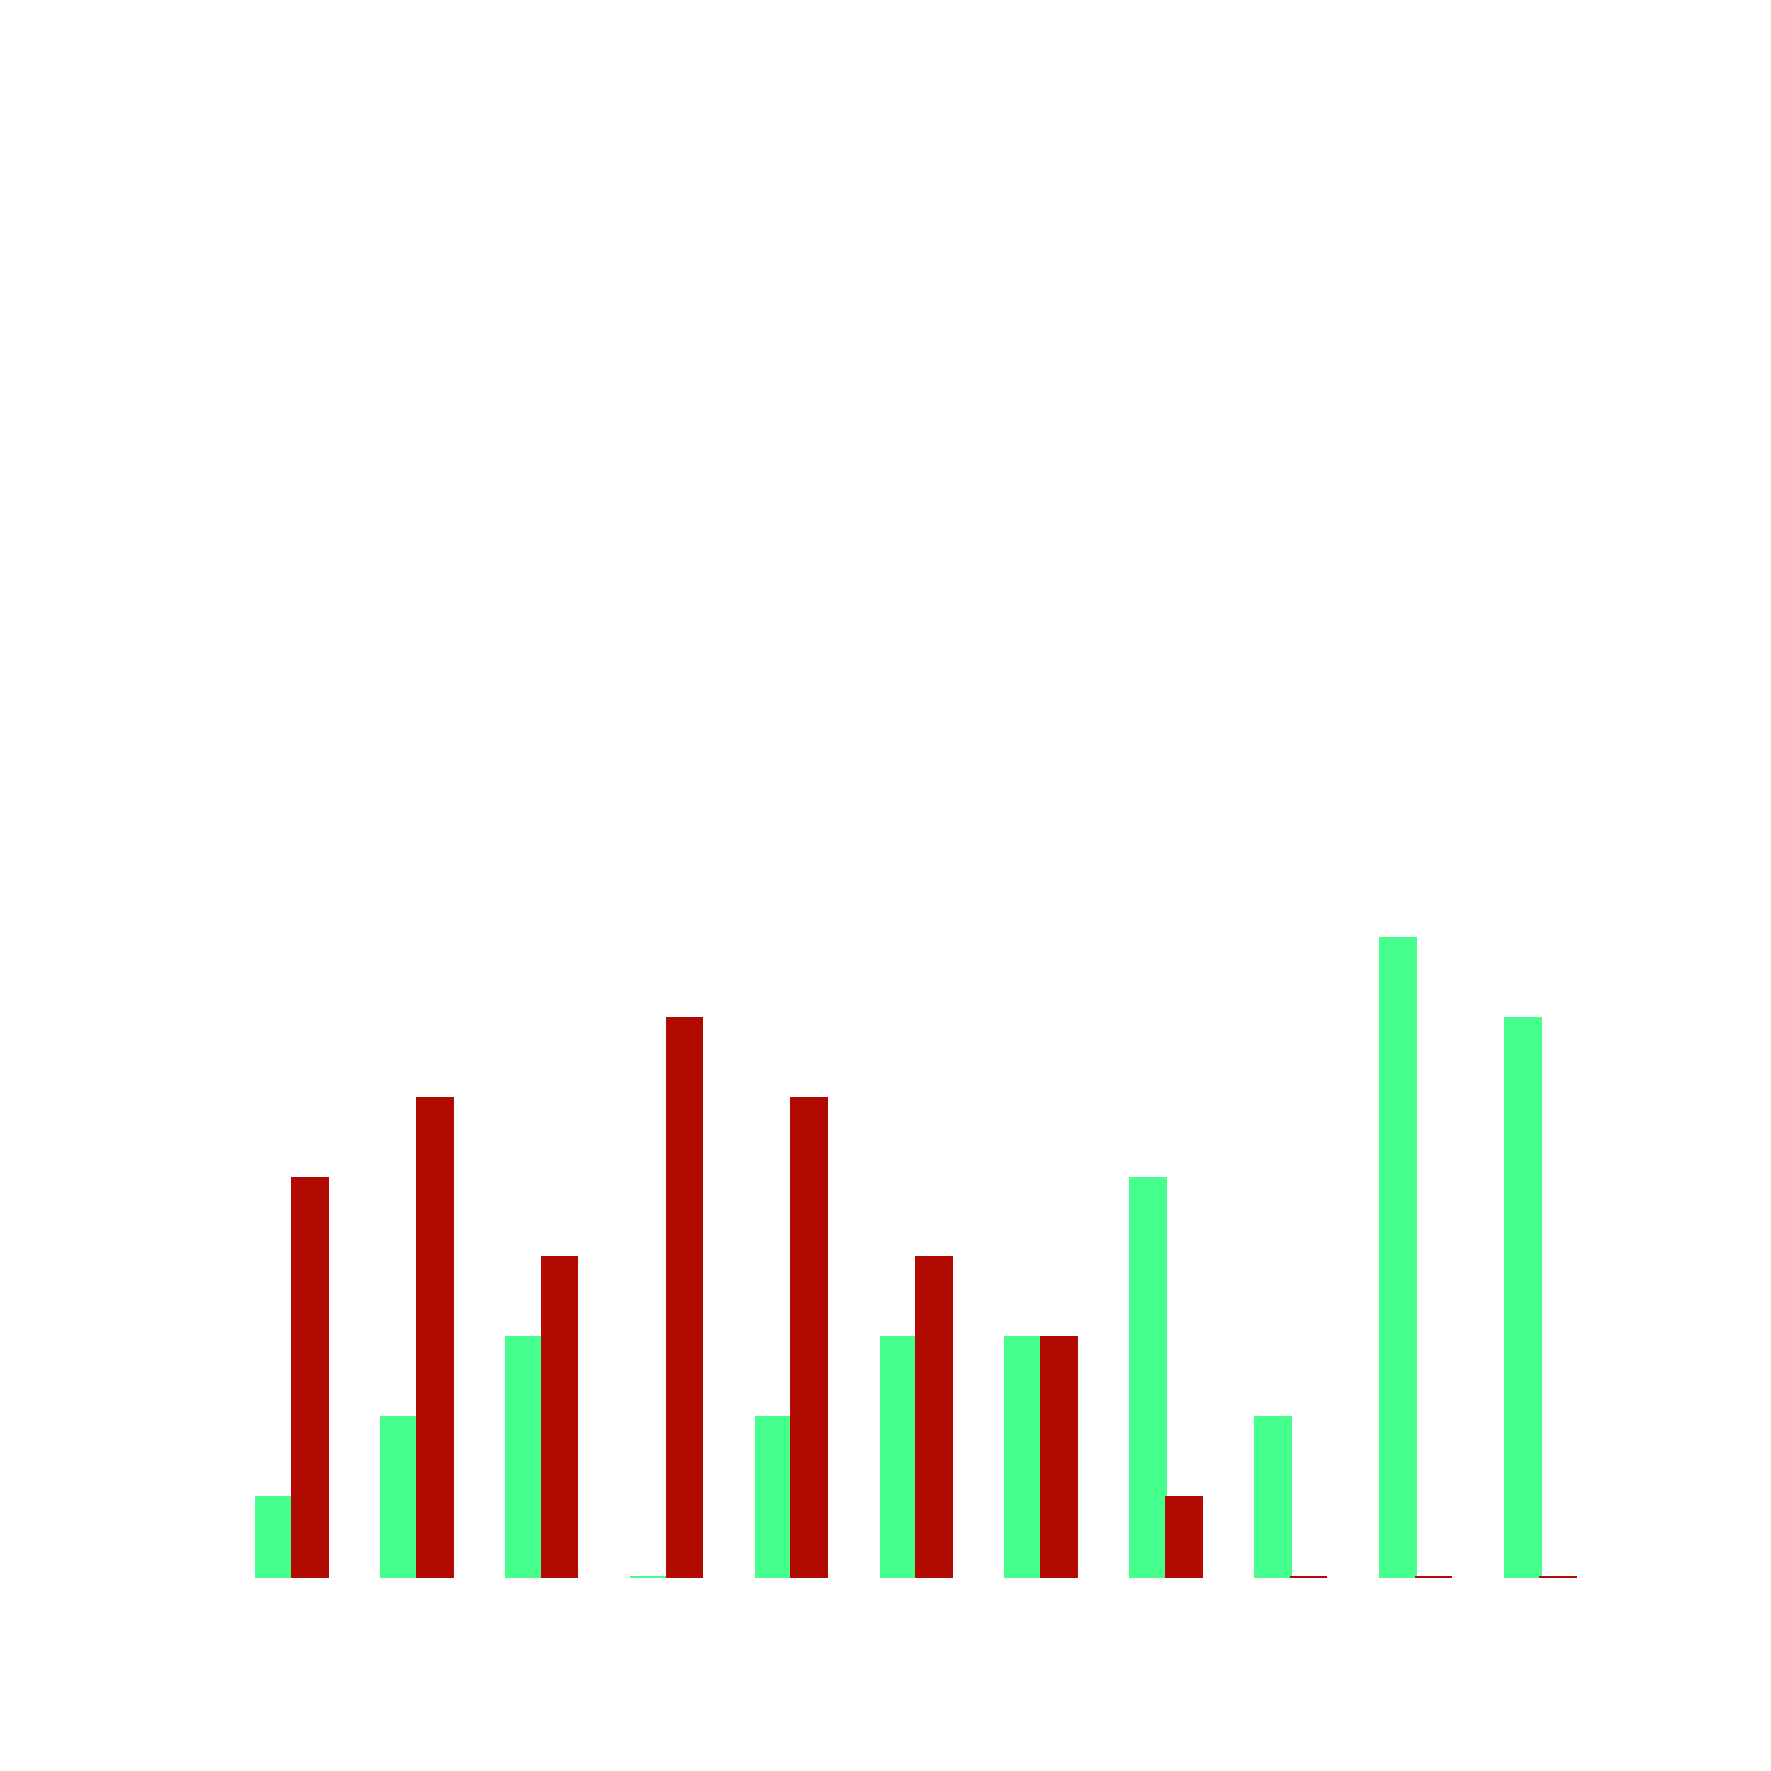
\includegraphics[width=.24\linewidth]{gfx/appendix/xp4_note_3}\label{fig:xp4_note_1c}}
        \subfloat[subject 4]
        {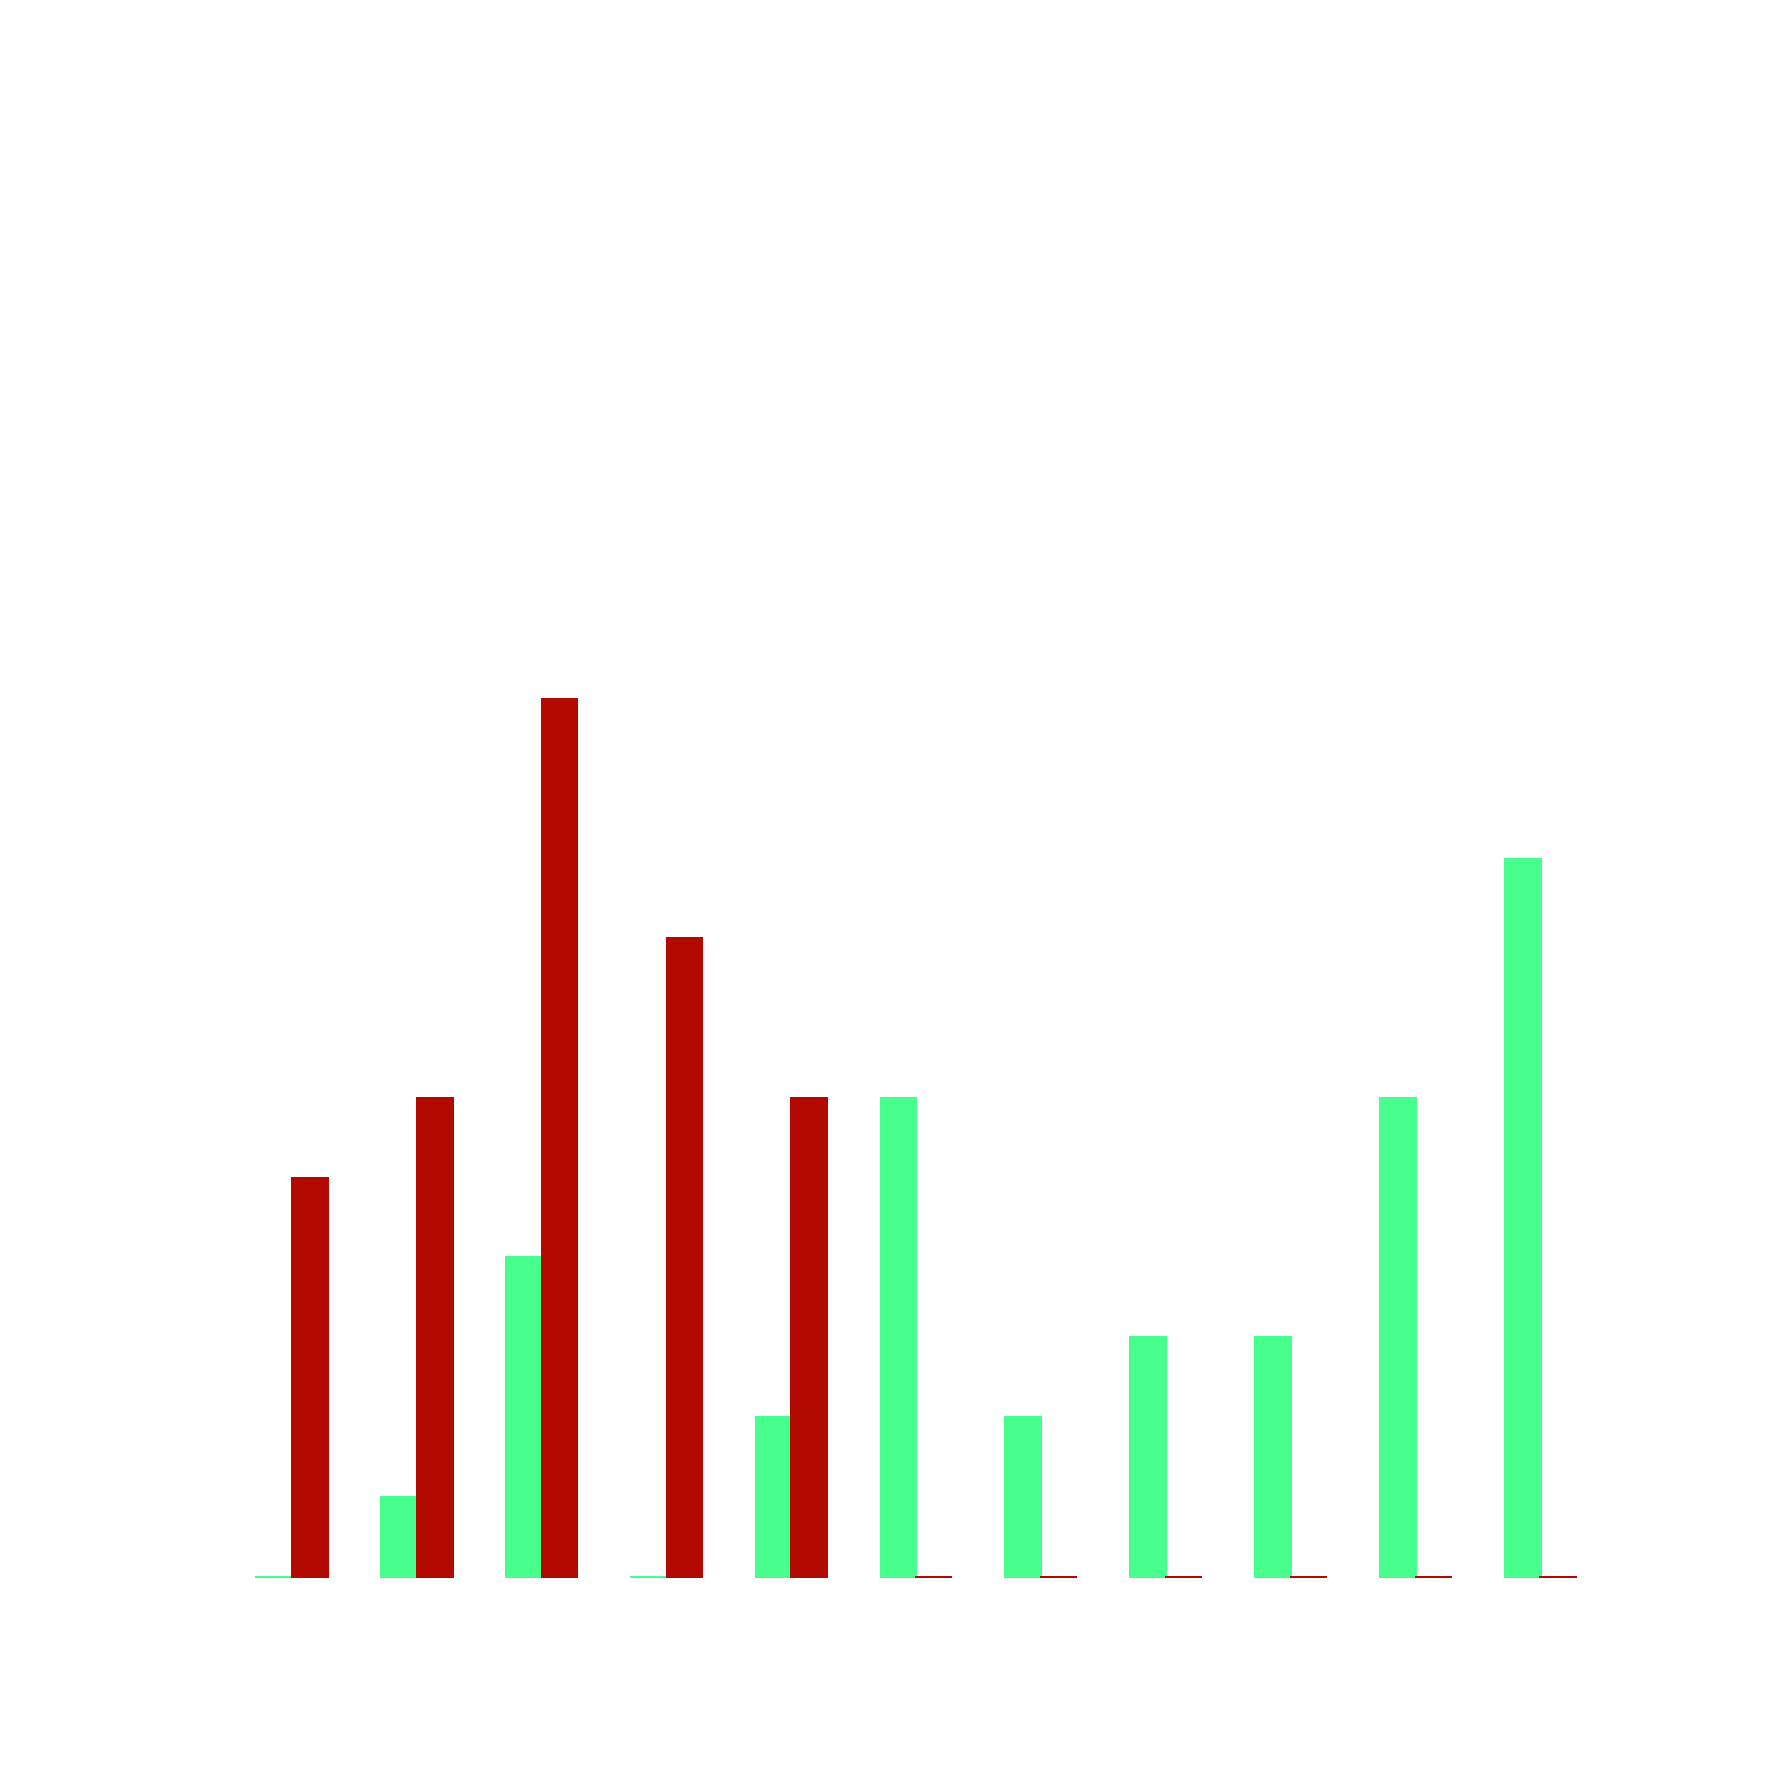
\includegraphics[width=.24\linewidth]{gfx/appendix/xp4_note_4}\label{fig:xp4_note_1d}} \par
        \subfloat[subject 5]
        {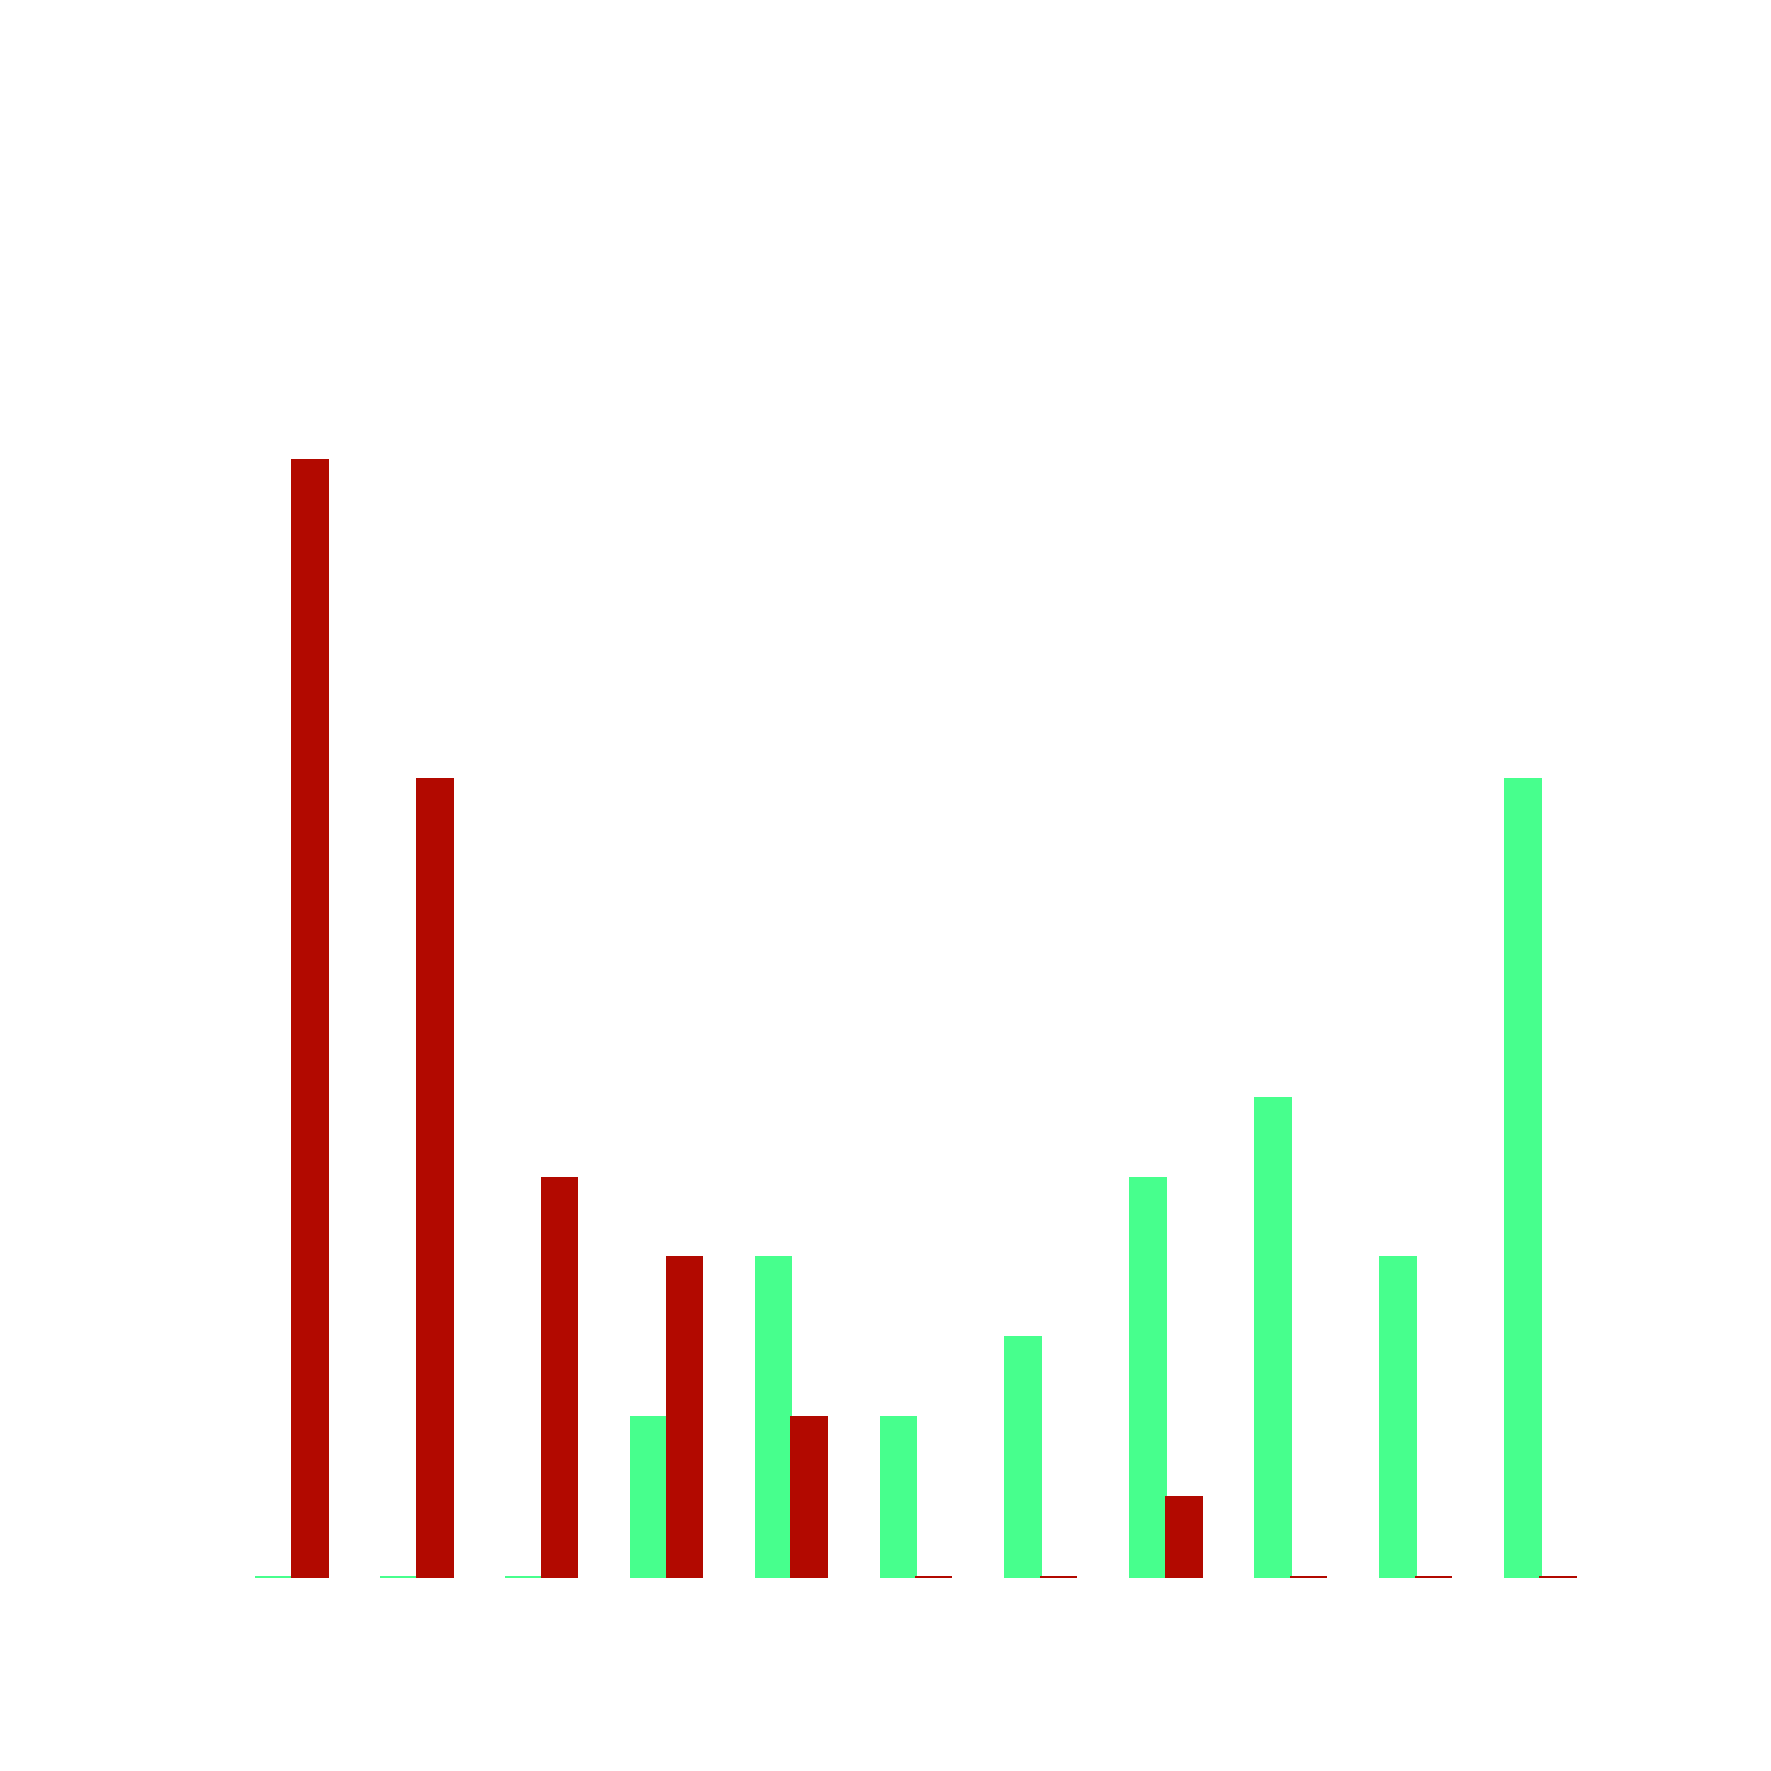
\includegraphics[width=.24\linewidth]{gfx/appendix/xp4_note_5}\label{fig:xp4_note_1e}}
        \subfloat[subject 6]
        {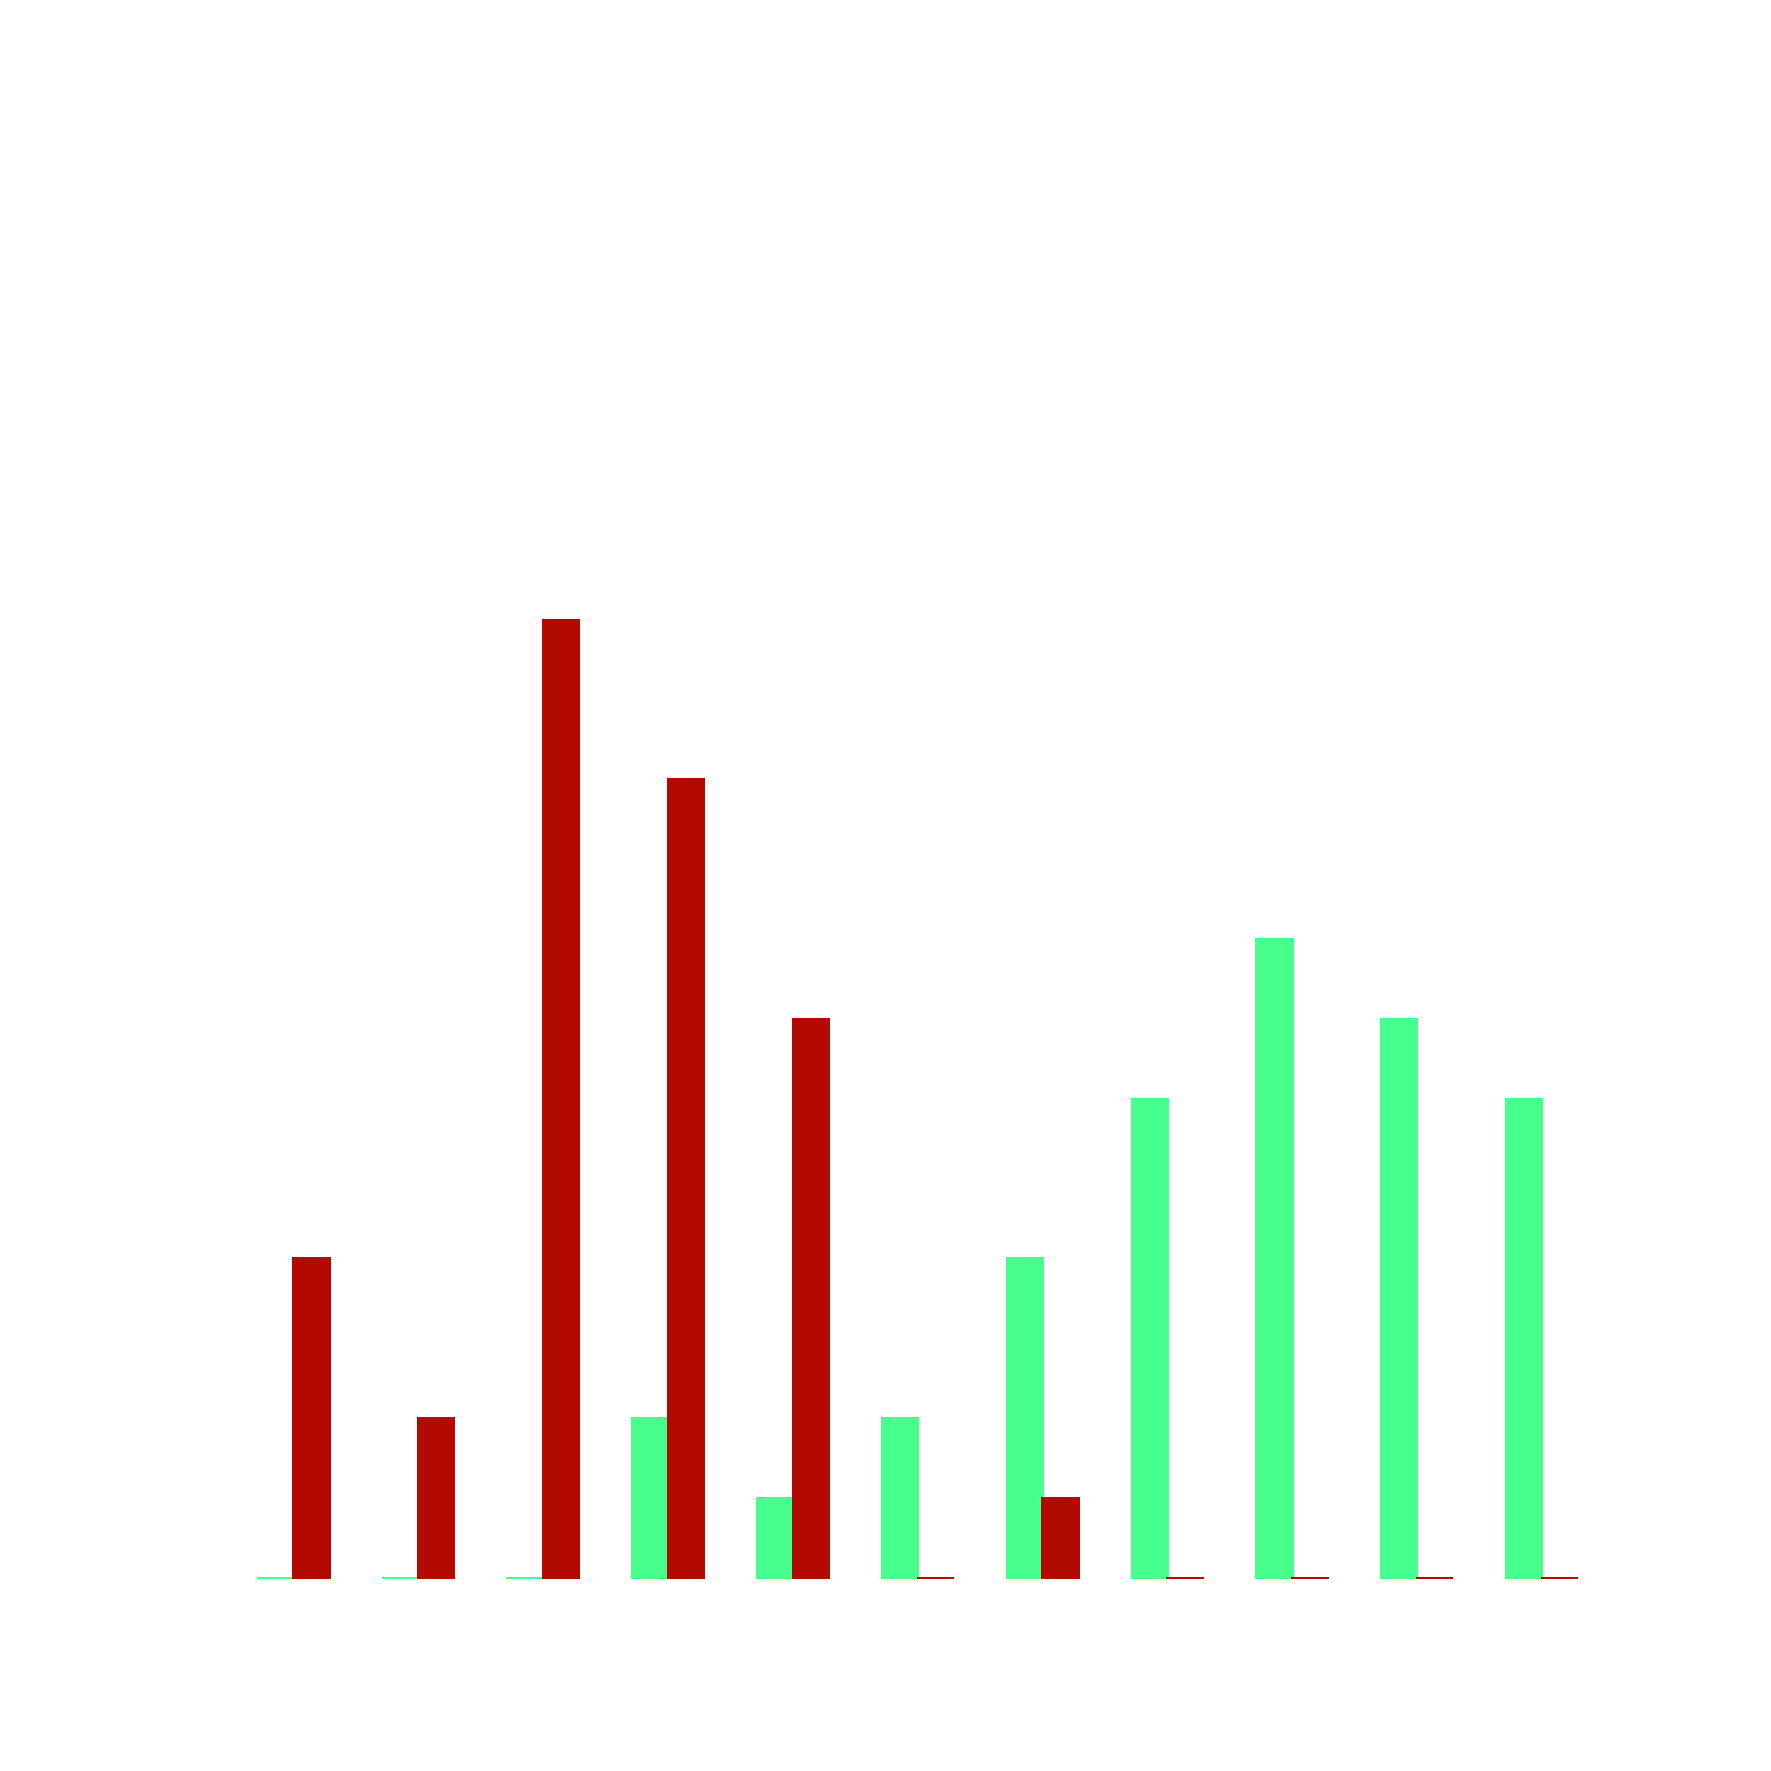
\includegraphics[width=.24\linewidth]{gfx/appendix/xp4_note_6}\label{fig:xp4_note_1f}}
        \subfloat[subject 7]
        {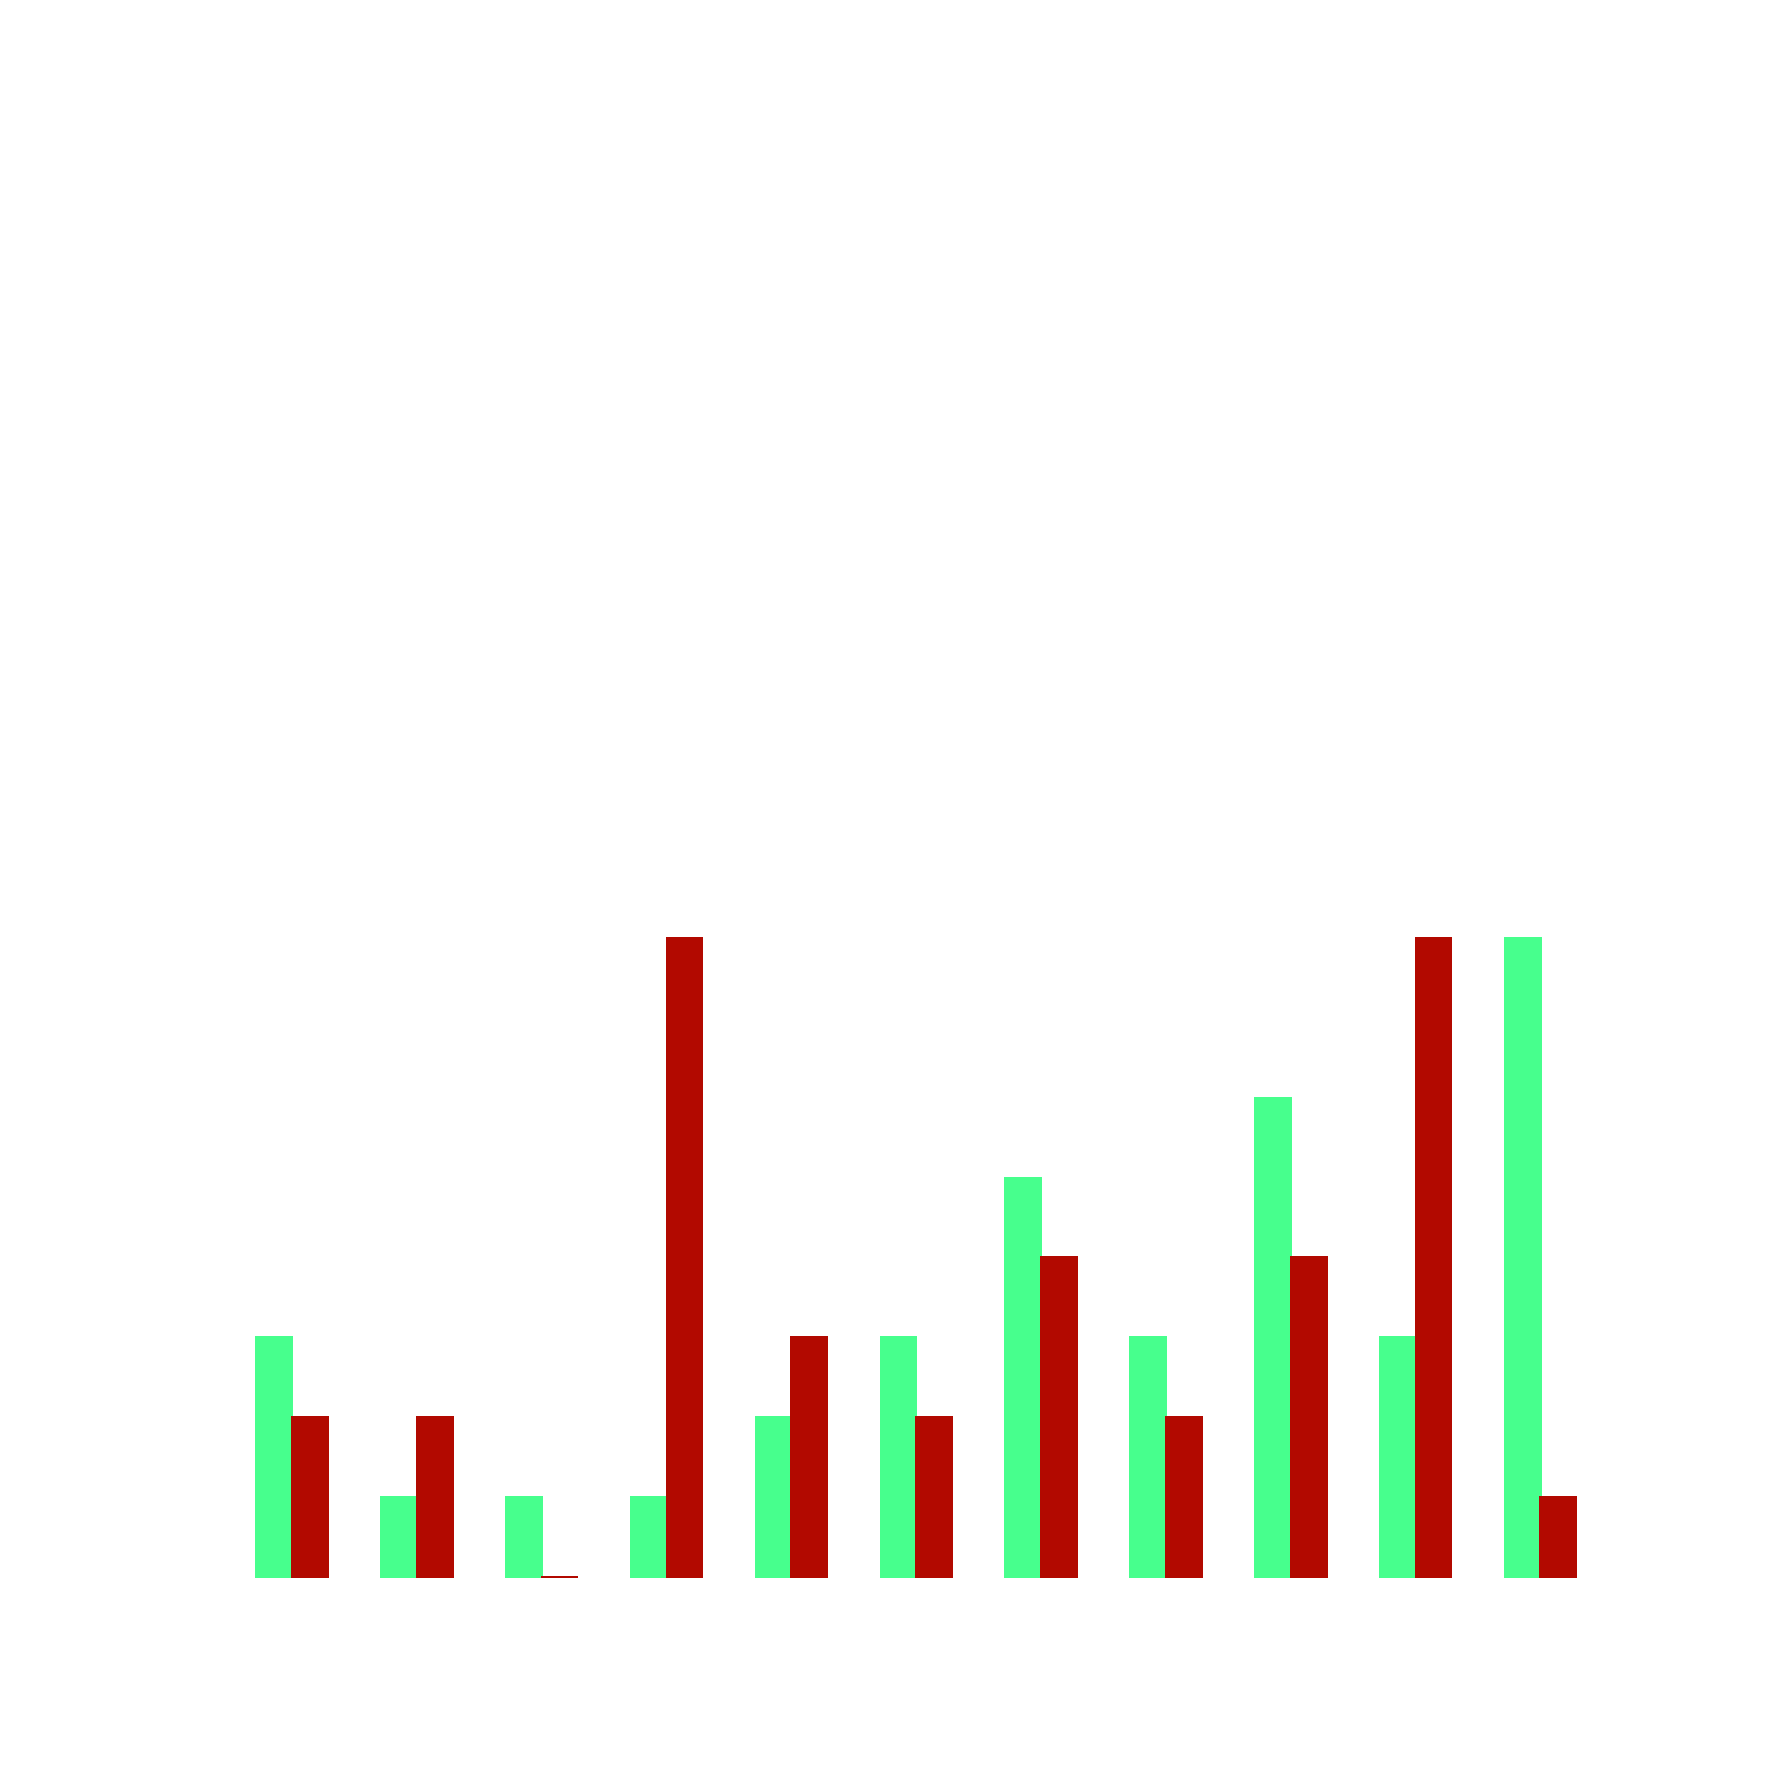
\includegraphics[width=.24\linewidth]{gfx/appendix/xp4_note_7}\label{fig:xp4_note_1g}}
        \subfloat[subject 8]
        {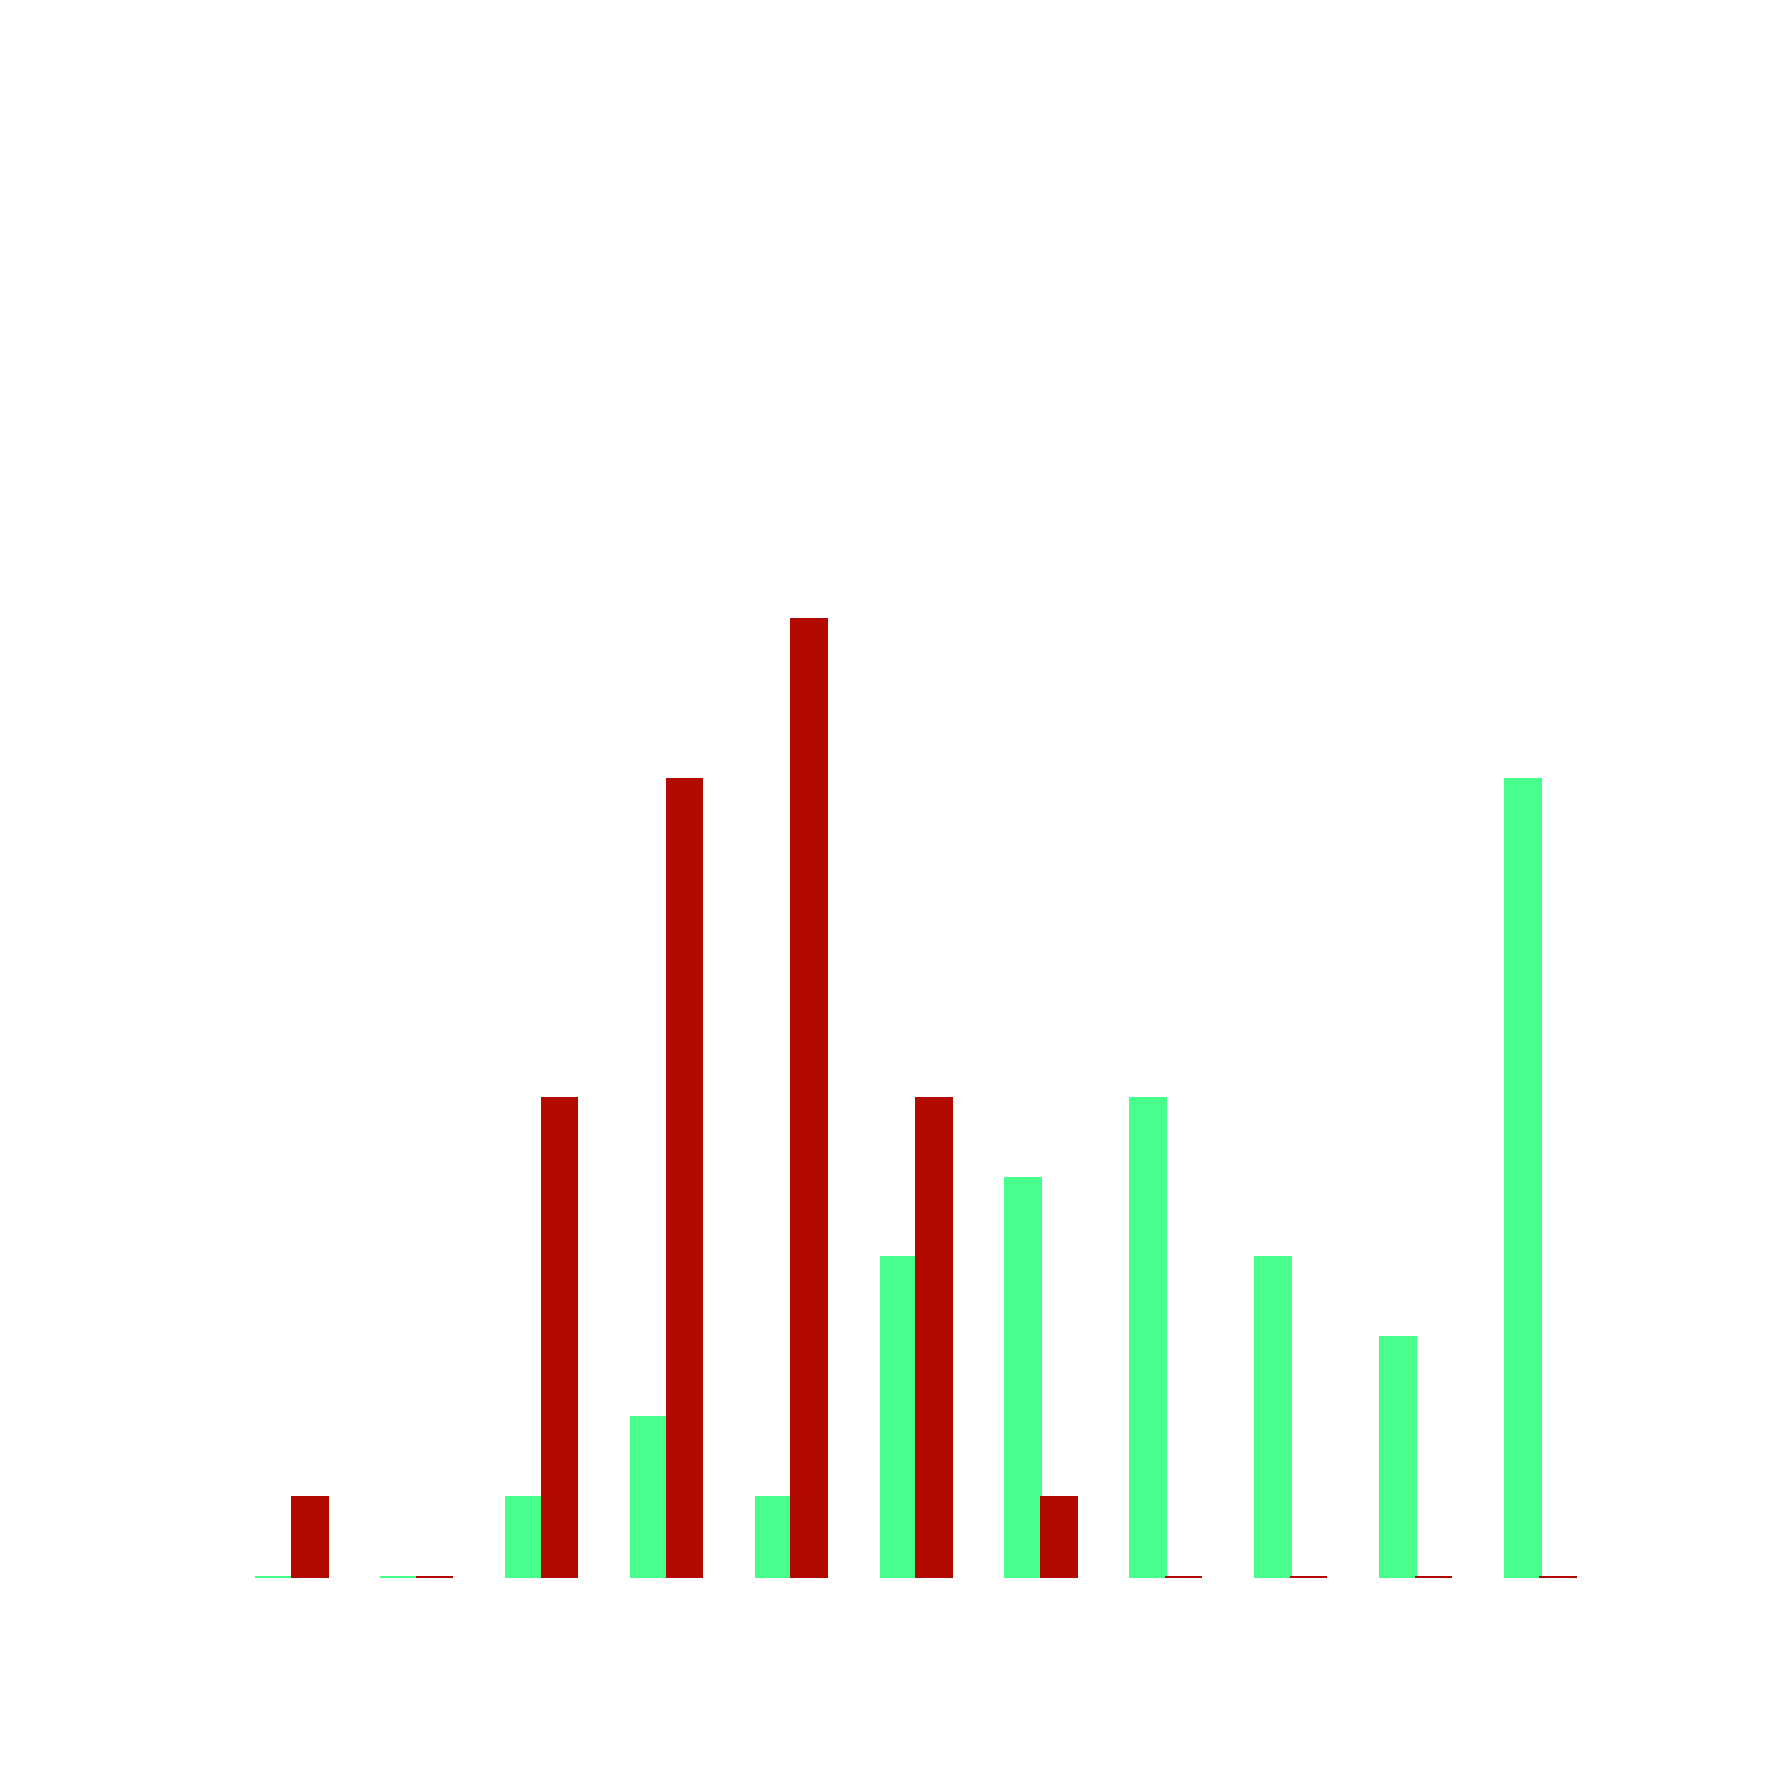
\includegraphics[width=.24\linewidth]{gfx/appendix/xp4_note_8}\label{}} \par
        \subfloat[subject 9]
        {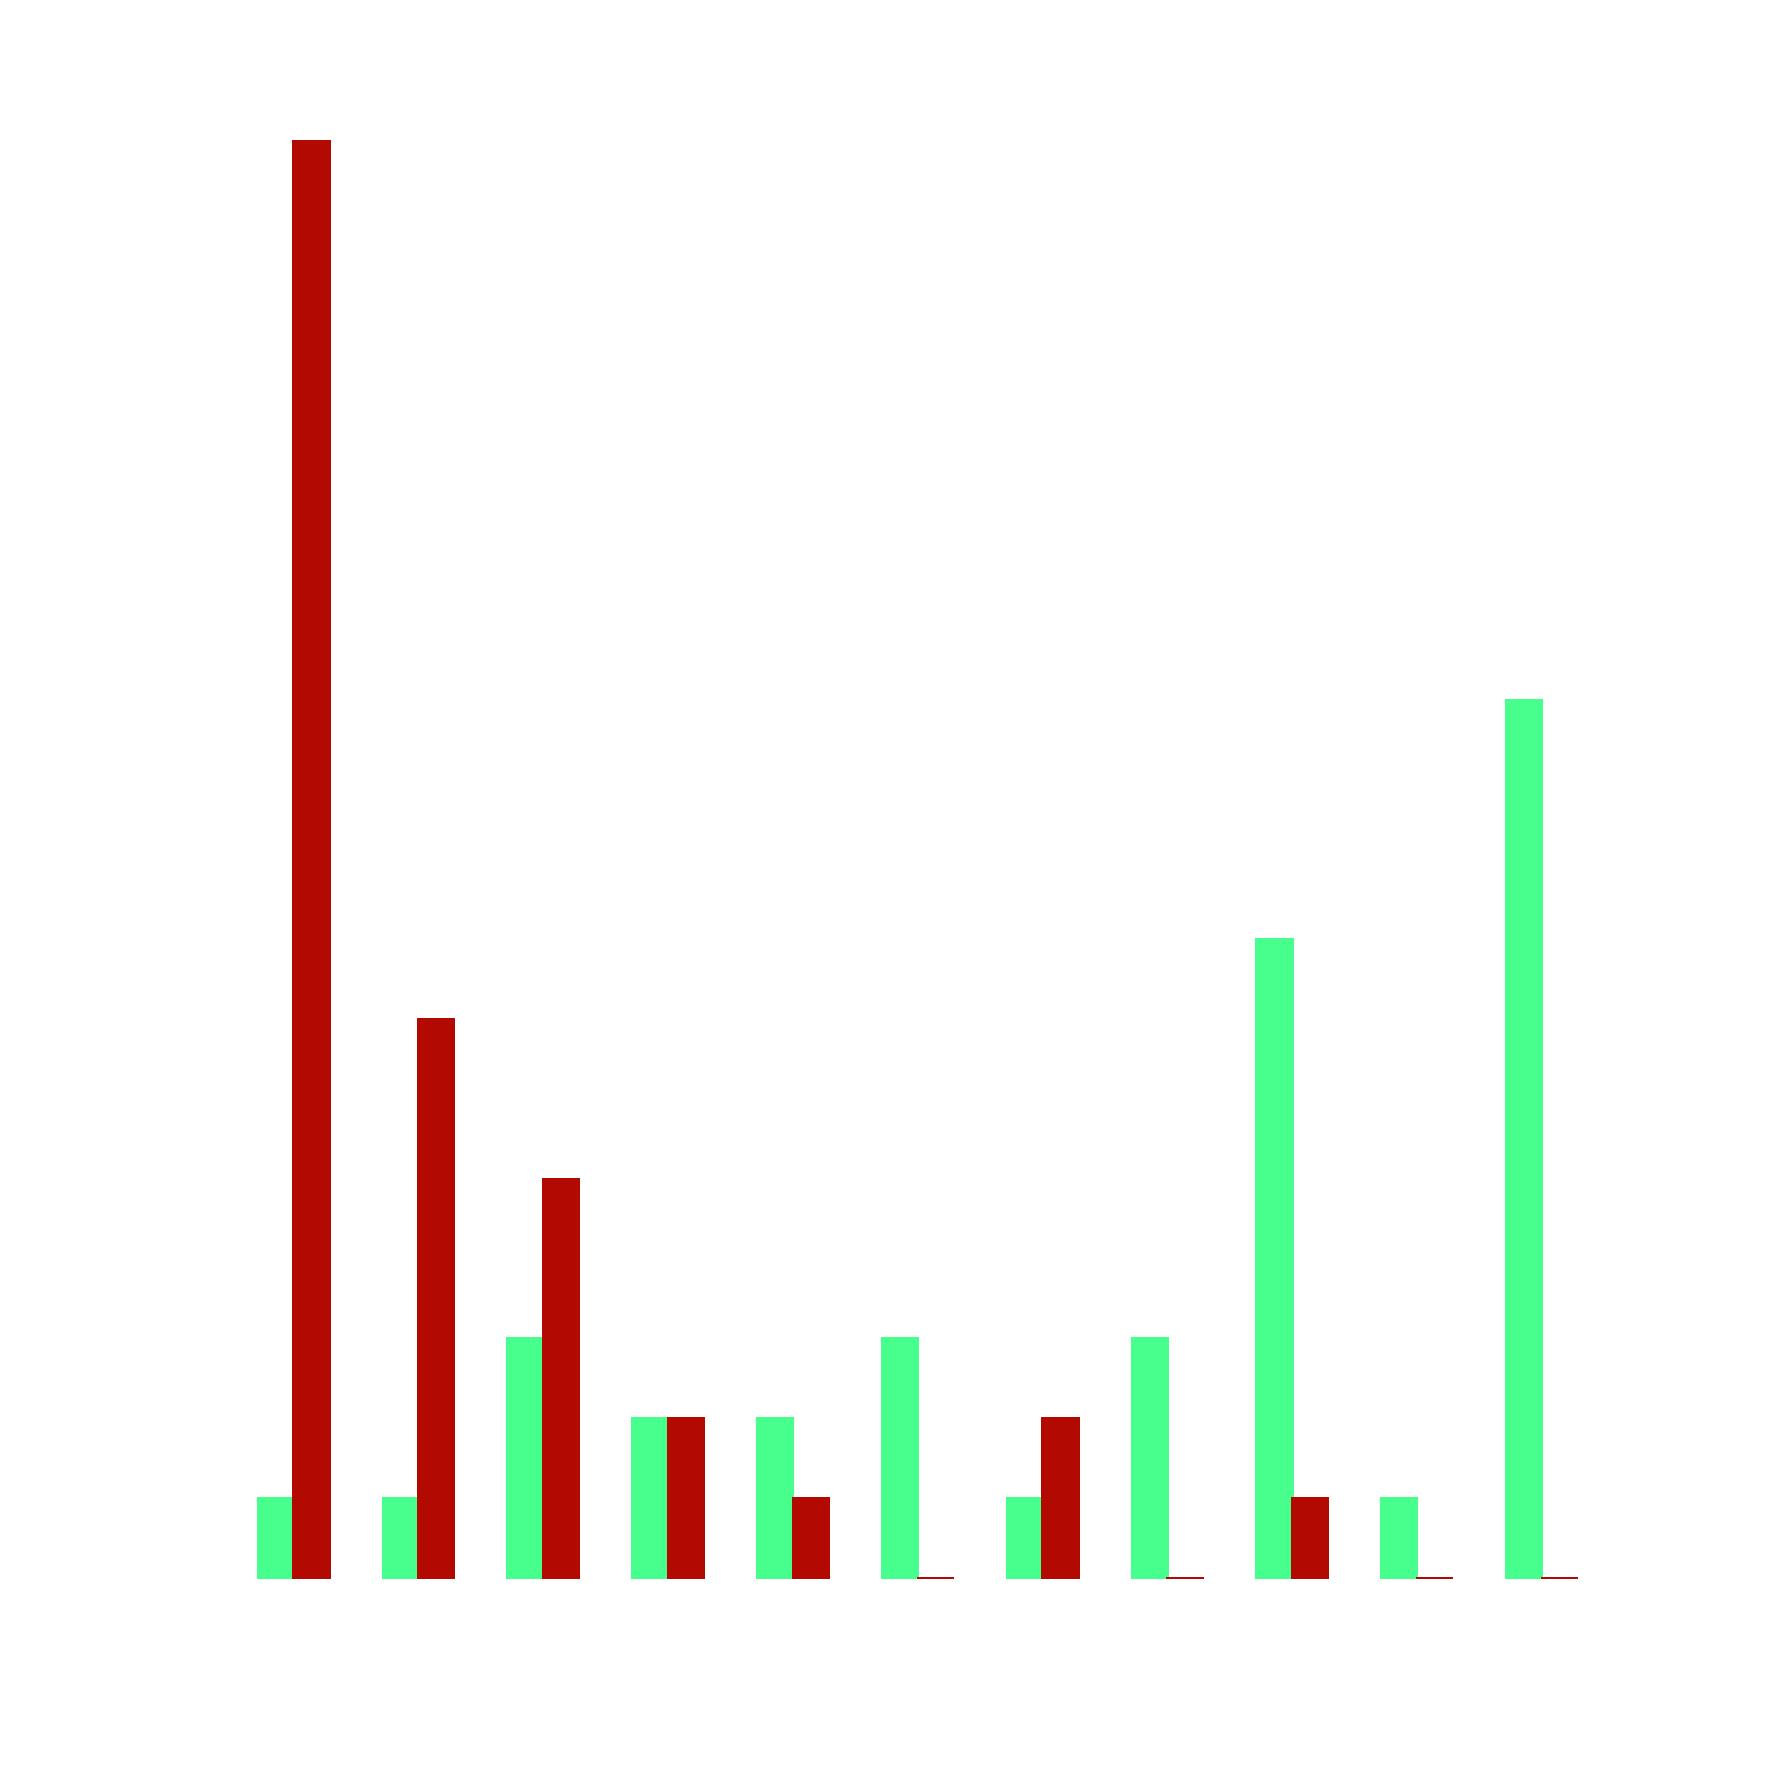
\includegraphics[width=.24\linewidth]{gfx/appendix/xp4_note_9}\label{fig:xp4_note_1i}}
        \subfloat[subject 10]
        {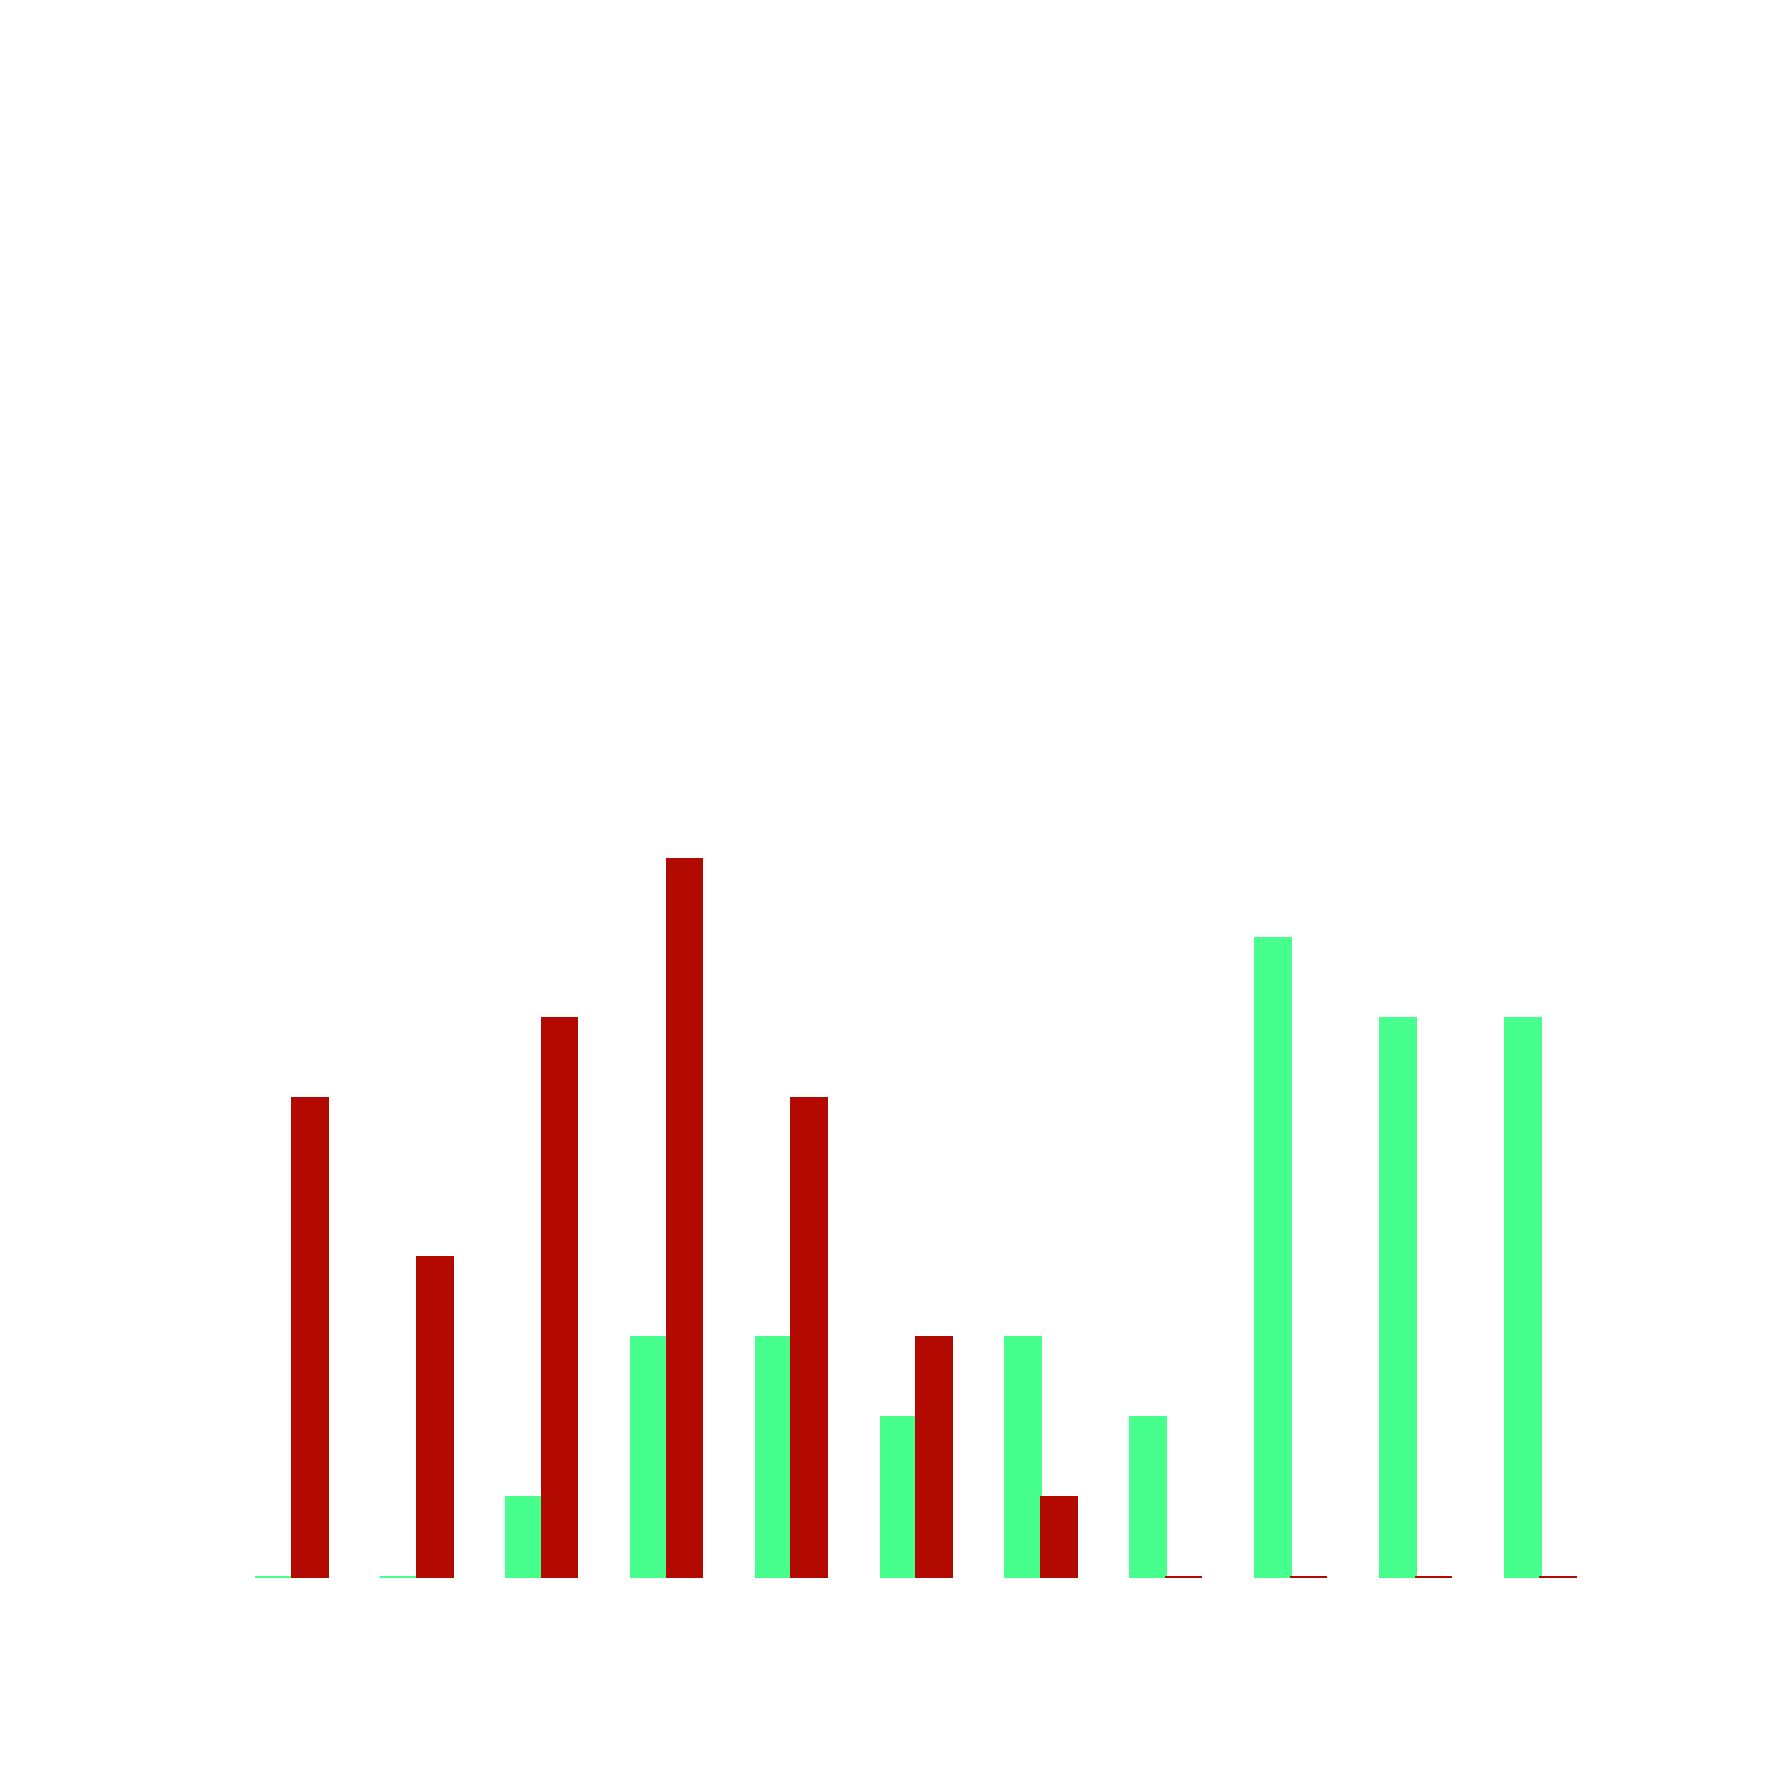
\includegraphics[width=.24\linewidth]{gfx/appendix/xp4_note_10}\label{fig:xp4_note_1j}}
        \subfloat[subject 11]
        {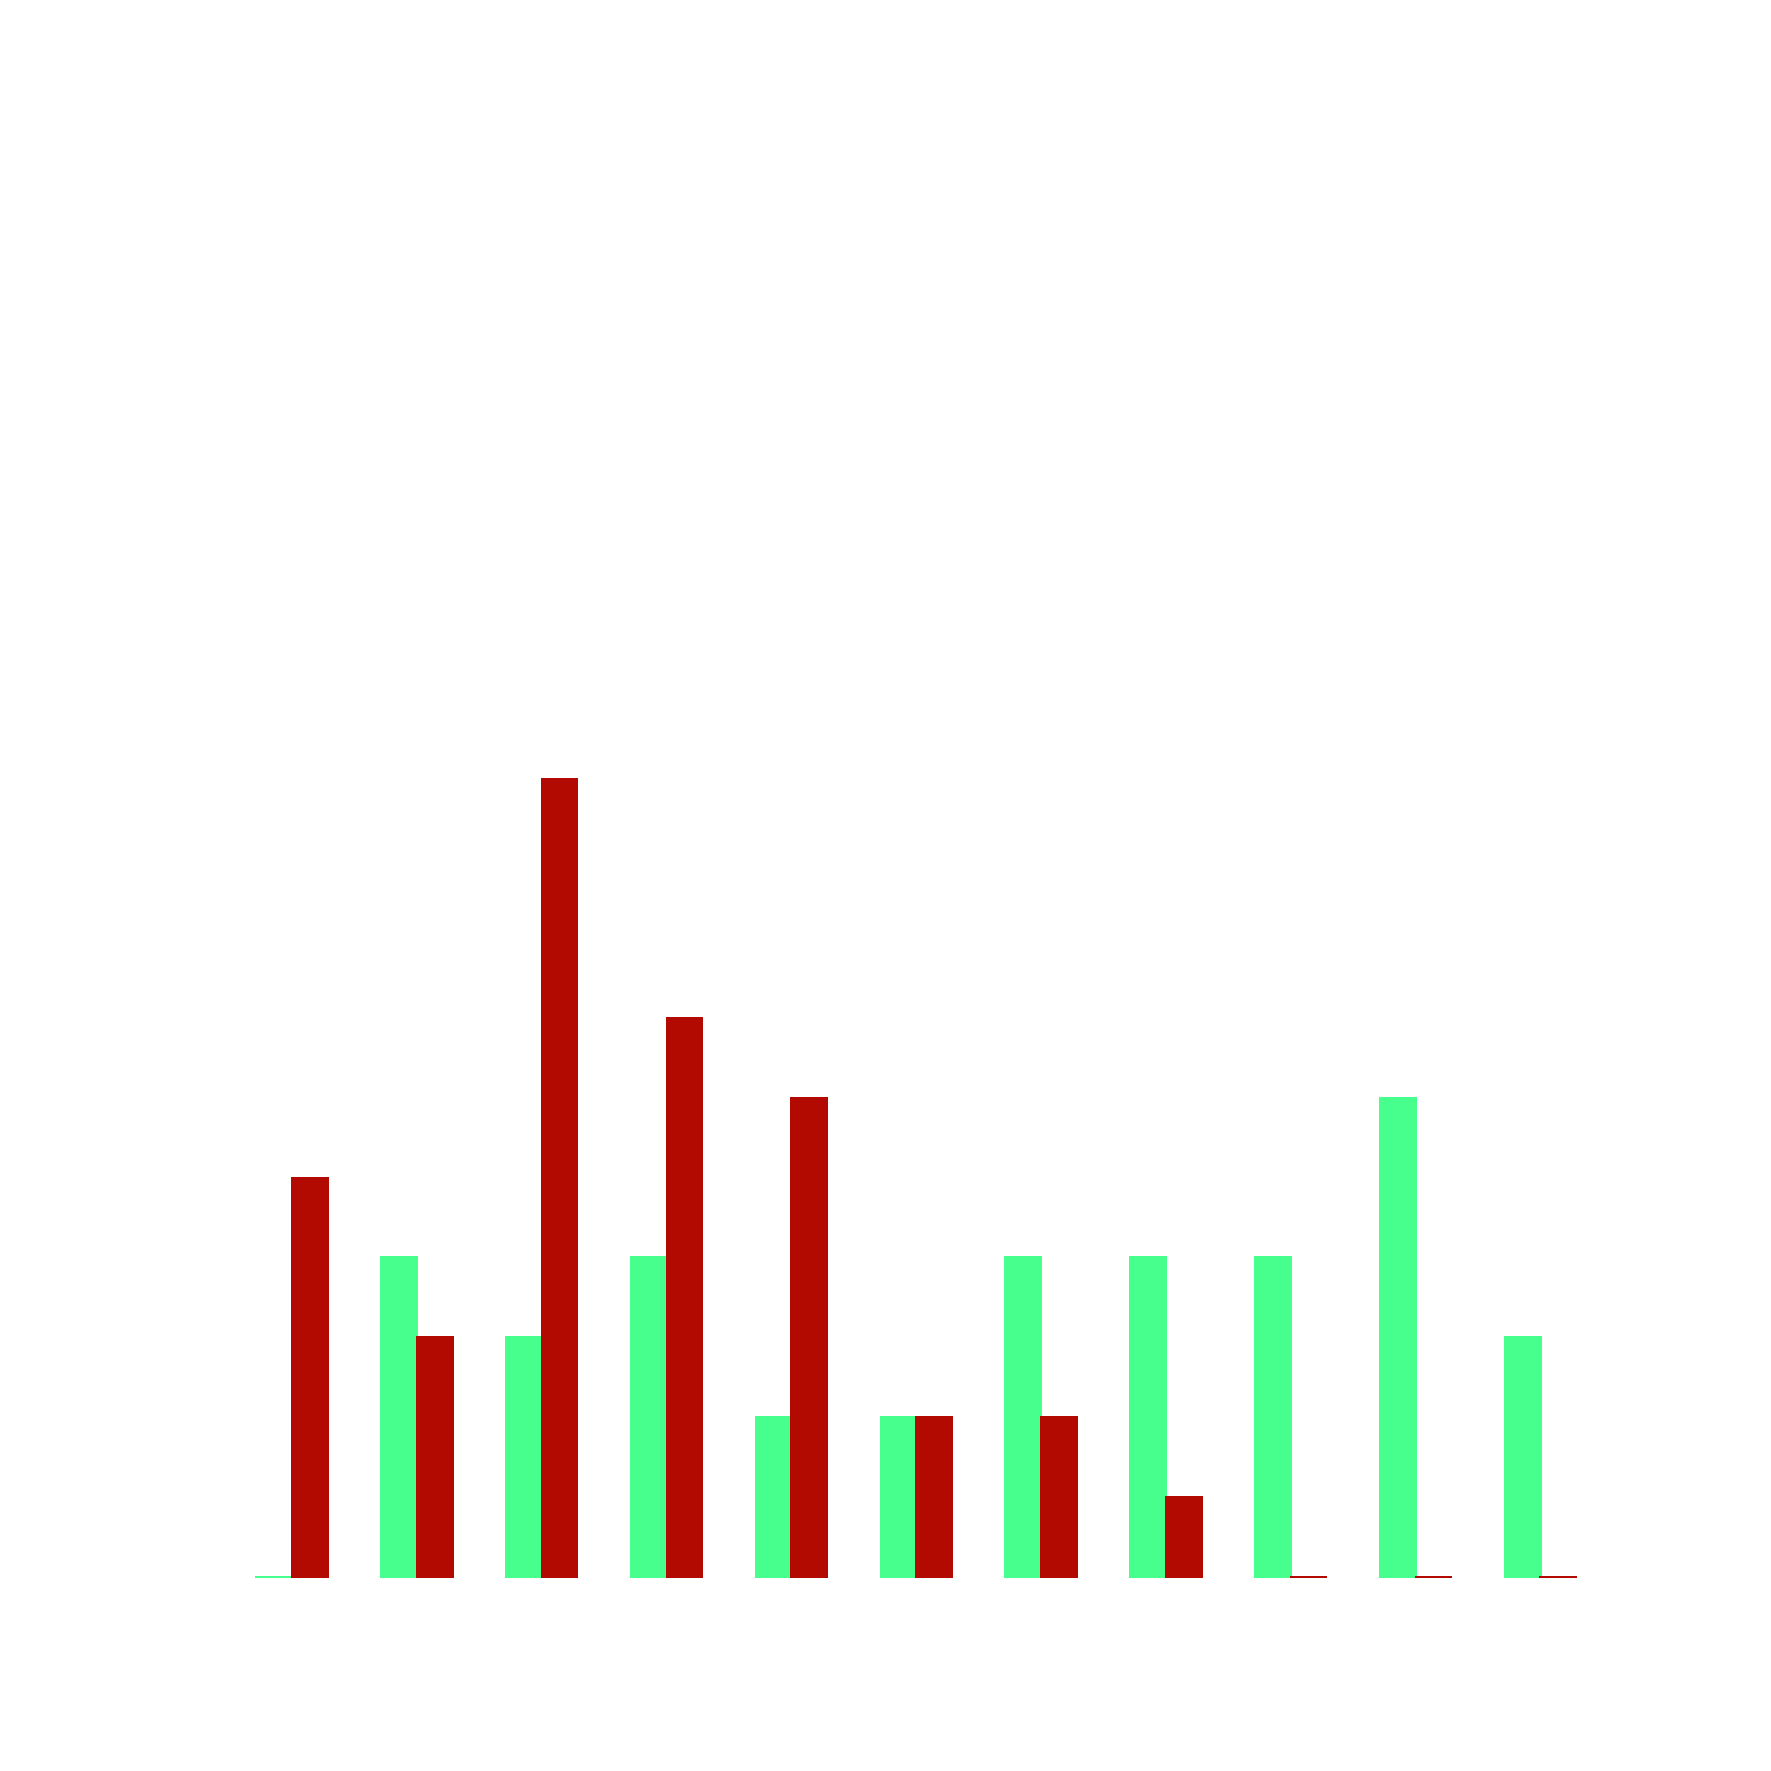
\includegraphics[width=.24\linewidth]{gfx/appendix/xp4_note_11}\label{fig:xp4_note_1z}}
        \subfloat[subject 12]
        {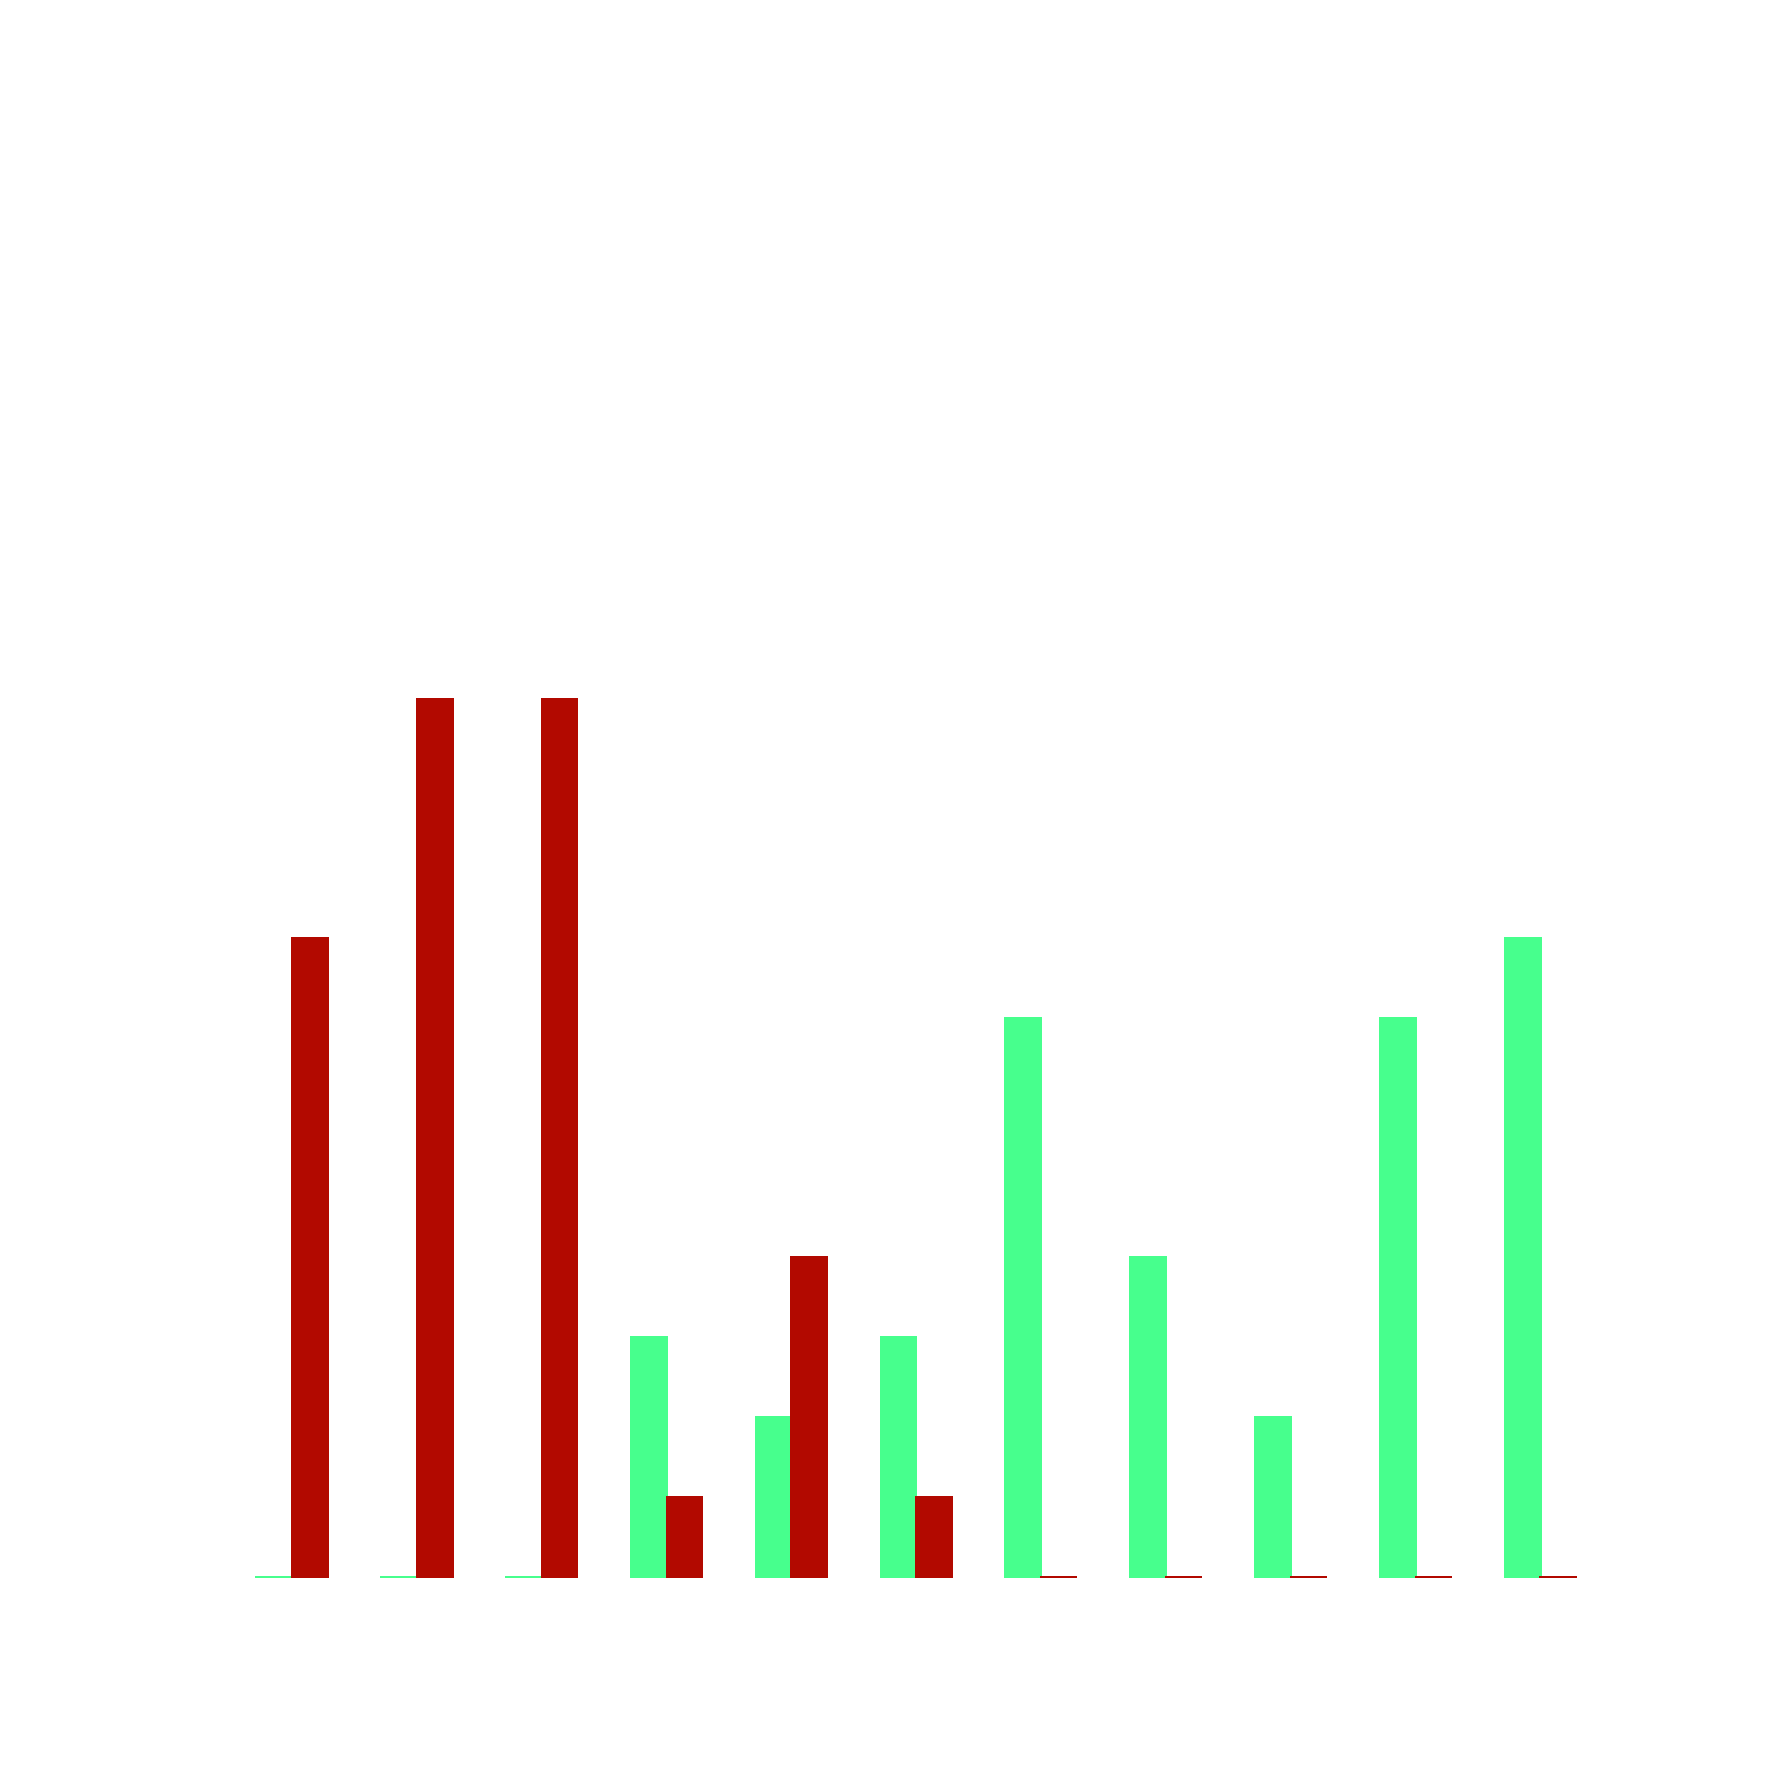
\includegraphics[width=.24\linewidth]{gfx/appendix/xp4_note_12}\label{fig:xp4_note_1l}}
        \caption{Distribution of scores given par the subjects during experiment 2 for i/am-scenes (green) et ni/am-scenes (red). The horizontal axis is, from left to right, the 11-point bipolar semantic scale ranging from -5 (non-ideal / very unpleasant) to +5 (ideal / very pleasant).}\label{fig:xp4_note_1}
\end{figure}

\end{document}
